\documentclass[bibtotoc]{scrreprt}
\usepackage[utf8]{inputenc}
\usepackage[T1]{fontenc}
\usepackage[british]{babel}
\usepackage{rotating}
\usepackage{graphicx}
\usepackage{subcaption}
\usepackage{caption}
\usepackage{wrapfig} % For wrapping figures in text.
\usepackage{float}	% For placing figures in minipages
\usepackage[hidelinks,linktocpage=true]{hyperref}
\usepackage{xcolor}
\usepackage{lipsum}
\usepackage{comment}
\usepackage{tabularx}
\usepackage{longtable}
\usepackage{multirow}
\usepackage{booktabs}
\usepackage{enumitem}
\usepackage[toc,page]{appendix}
\usepackage{ccicons} % The Creative Commons Icons
\usepackage{perpage} %the perpage package
\usepackage{float}
\usepackage{amsmath}
\usepackage{amsfonts} 
\usepackage[capitalise,nameinlink,noabbrev]{cleveref}
\MakePerPage{footnote} %the perpage package command

% Add remark without numbering for writing notes

\usepackage{amsthm}
\theoremstyle{remark}
\newtheorem*{remark}{\textcolor{red}{\textbf{Remark}}}

% extend cref with footnote marks
\crefformat{footnote}{#2\footnotemark[#1]#3}

% Add dummy phantomsection for use
\providecommand\phantomsection{}

% Referemces
\usepackage[backend=biber,sorting=nyt,style=apa]{biblatex}
\addbibresource{bibliography.bib}
\usepackage{csquotes}
\usepackage{citeall}

% option 1 with useprefix=false
% https://latex.org/forum/viewtopic.php?t=23146
\makeatletter
\AtBeginDocument{\toggletrue{blx@useprefix}}
\AtBeginBibliography{\togglefalse{blx@useprefix}}
\makeatother

% Option 2 with useprefix=on
%\DeclareSortingNamekeyTemplate{
%	\keypart{
%		\namepart{family}
%	}
%	\keypart{
%		\namepart{prefix}
%	}
%	\keypart{
%		\namepart{given}
%	}
%	\keypart{
%		\namepart{suffix}
%	}
%}%

%\renewbibmacro*{begentry}{\midsentence}

% Commands
\newcommand{\needsref}{\textcolor{red}{\textbf{(NEEDS REF)}}}

% glossaries
\usepackage[toc,acronym,style=altlisthypergroup,nonumberlist]{glossaries}
\makeglossary
% Glossary
\newglossaryentry{ps}
{
	name={public sector},
	description={The Public Sector is comprised of organisations that are owned and operated by the government and exist to provide services for its citizens.}
}
\newglossaryentry{artefact}
{
	name={artefact},
	plural={artefacts},
	description={An artefact is used to describe something artificial, or constructed by humans, as opposed to something that occurs naturally}
}
\newglossaryentry{agile}
{
	name=agile,
	plural={agility},
	description={The ability to adjust before failure happens}
}
\newglossaryentry{agility}
{
	name={agility},
	description={The state of being agile}
}
\newglossaryentry{antifragile}
{
	name={antifragile},
	plural={antifragility},
	description={The ability to strive for and evolve under stress}
}
\newglossaryentry{antifragility}
{
	name={antifragility},
	description={The state of being antifragile}
}
\newglossaryentry{fragile}
{
	name=fragile,
	plural={fragility},
	description={The quality of being easily broken or destroyed}
}
\newglossaryentry{fragility}
{
	name={fragility},
	description={The state of being fragile}
}
\newglossaryentry{resilient}
{
	name=resilient,
	plural={resiliency},
	description={The ability to recover from failure}
}
\newglossaryentry{resiliency}
{
	name={resiliency},
	description={The state of being resilient}
}
\newglossaryentry{robust}
{
	name=robust,
	plural={robustness},
	description={The ability to resist failure}
}
\newglossaryentry{robustness}
{
	name={robustness},
	description={The state of being robust}
}
\newglossaryentry{volatile}
{
	name={volatile},
	description={Likely to change in a very sudden or extreme way}
}
\newglossaryentry{volatility}{
	name={volatility},
	description={The state of being volatile},
}
\newglossaryentry{uncertain}
{
	name=uncertain,
	description={Not known beyond doubt}
}
\newglossaryentry{uncertainty}{
	name={uncertainty},
	description={the state of being uncertain}
}
\newglossaryentry{complex}
{
	name=complex,
	description={A whole made up of complicated or interrelated parts}
}
\newglossaryentry{ambiguous}
{
	name=ambiguous,
	description={Not expressed or understood clearly}
}
\newglossaryentry{stressor}
{
	name={stressor},
	plural={stressors},
	description={When systems are performing effectively, they are in a predetermined condition and conversely when they are not functioning correctly, they are in an unintended state. An unintended condition can be known or unknown. Stressors are forces that threaten to transfer a system from an intended to an unintended condition. In short you can also say that a stressor is an event from outside the system that causes stress}
}
\newglossaryentry{glos_fmea}
{
	name={failure mode effects analysis},
	text={Failure Mode Effects Analysis},
	description={Is a Six Sigma technique that helps manage quality in a system by investigating how the system will cope with failure}
}
\newglossaryentry{entropy}
{
	name={entropy},
	description={The entropy of the universe increases in all natural processes. Isolated systems tend towards greater disorder and entropy is a measure of that disorder}
}
\newglossaryentry{digitaltransformation}{
	name={digital transformation},
	description={Digital Transformation is the application of digital capabilities to processes, products, and assets to improve efficiency, enhance customer value, manage risk, and uncover new monetisation opportunities.}
}
\newglossaryentry{archframework}{
	name={architecture framework},
	description={An enterprise architecture framework (EA framework) defines how to create and use an enterprise architecture. An architecture framework provides principles and practices for creating and using the architecture description of a system. It structures architects' thinking by dividing the architecture description into domains, layers, or views.}
}
\newglossaryentry{immemorial}{
	name={immemorial},
	description={Reaching beyond the limits of memory, tradition, or recorded history}
}
\newglossaryentry{disintermediation}{
	name={disintermediation},
	description={Disintermediation is the process of cutting out one or more middlemen from a transaction, supply chain, or decision-making process}
}
\newglossaryentry{arduous}{
	name={arduous},
	description={Hard to accomplish or achieve}
}
\newglossaryentry{domain}{
	name={domain},
	plural={domains},
	description={A field of action, thought, influence, etc.: The Domain of Science}
}
\newglossaryentry{convex}{
	name={convex},
	description={Being a continuous function or part of a continuous function with the property that a line joining any two points on its graph lies on or above the graph. In the antifragile theory more upside than downside}
}
\newglossaryentry{concave}{
	name={cavex},
	description={Being a continuous function or part of a continuous function with the property that a line joining any two points on its graph lies below the graph. In the antifragile theory more downside than upside}
}
\newglossaryentry{personalmastery}{
	name={personal mastery},
	description={Personal mastery is a discipline of continually clarifying and deepening our personal vision, of focusing our energies, of developing patience, and of seeing reality objectively}
}
\newglossaryentry{sharedmentalmodel}{
	name={shared mental model},
	plural={shared mental models},
	description={Mental models are deeply ingrained assumptions, generalizations, or even pictures of images that influence how we understand the world and how we take action}
}
\newglossaryentry{buildingsharedvision}{
	name={building shared vision},
	description={A practice of unearthing shared pictures of the future that foster genuine commitment and enrollment rather than compliance}
}
\newglossaryentry{teamlearning}{
	name={team learning},
	description={Team learning starts with 'dialogue', the capacity of members of a team to suspend assumptions and enter into genuine 'thinking together'}
}
\newglossaryentry{systemsthinking}{
	name={systems thinking},
	description={a discipline for seeing wholes. It is a framework for seeing inter-relationships rather than things, for seeing patterns of change rather than static snapshots. The fifth discipline of Senge states that it must contain personal mastery, shared mental models, building shared vision, and team learning for a learning organisation.}
}
\newglossaryentry{attenuatevariety}{
	name={attenuate variety},
	description={Dampening or reducing the possible outcomes / states. A light that can be turned on and off has the variety of 2. Your hand during Rock, paper, scissors has the variety or 3}
}
\newglossaryentry{amplifyvariety}{
	name={amplify variety},
	description={Amplifying or increasing the possible outcomes / states. A light that can be turned on and off has the variety of 2. Introducing the possibility of setting the light intensity increases the possible states}
}
\newglossaryentry{resourcestoinvest}{
	name={resources to invest},	
	description={Oportonies can only be seized when there are resources free to do see. This can be money but also time and labour. To Survive a black swan investment should be possible}
}
\newglossaryentry{senecabarbell}{
	name={seneca's barbell},
	text={Seneca's barbell},	
	description={To be antifragile you need a robust sub-system to which 80\%/90\% predictable value with low risk is situated. The 20\%/10\% should be used for high return on investment activities}
}
\newglossaryentry{insertrandomness}{
	name={insert randomness},	
	description={When insert-low-level stress and fail fails delivers no issues the next step is to insert randomness into the systems. A great example of this is Chaos Engineering by Netflix or the HackerOne bug-bounty system}
}
\newglossaryentry{reducenaiveintervention}{
	name={reduce naive intervention},	
	description={Intervention based on a model and reductionistic logic and ignoring the experience. An example is not listening to the experienced but not so articulate employee, or by ignoring the balance nature has found in a ecosystem}
}
\newglossaryentry{skininthegame}{
	name={skin in the game},	
	description={Make certain that the one making the decision and doing the work has a pain and gain relation with the outcome. This goes beyond having a feedback system in place. This is goed beyond having KPI’s in place. An example is that when working Agile scrum, the product owner should be a co-worker in the team for whom the solution is being build}
}
\newglossaryentry{topdowncc}{
	name={top-down dommand \& control},
	text={Top-Down Command \& Control},
	description={Top-Down command and control is in an organisation that a employee is not free to decide to go left or right but has to follow orders. The careful design of an iPhone or a good pen is also an example of limited freedom of movement in the product itself}
}
\newglossaryentry{micromanagement}{
	name={micro-management},
	text={Micro-Management},
	description={Micro-management is about the freedom in the use of the product. When there are minitious working instructions available in a business process the employee has no freedom in the execution of the job. Another great example is a lego building block. It is engineered and fabricated into the greatest detail creating a building block that is almost completely robust. Lego has a very small resilience behaviour through engineering}
}
\newglossaryentry{redundancy}{
	name={redundancy},
	description={Redundancy is about having not a single point of failure by making use of duplication. An example is a backup electricity generators. Another example is local government as backup system of the central government}
}
\newglossaryentry{modularity}{
	name={modularity},
	description={Modularity is the degree that components may be separated and recombined, often with the benefit of flexibility. For example the finance team and the marketing team. Another example is the user-interface module and the data storage module}
}
\newglossaryentry{looselycoupled}{
	name={loosely coupled},
	description={Loosely coupled is the degree of dependency on the exact working of another module. For example when the color-schema of a website is changed it is preferred that this does not impact the functioning of the website. Another example is that when there are new employees introduced at the finance department the taste of the coffee changes. It is important to understand that there is always some degree of coupling}
}
\newglossaryentry{diversity}{
	name={diversity},
	description={Diversity is internally not being a mono-culture and externally having options. For example having two different coffee suppliers. Or having a diverse team}
}
\newglossaryentry{optionality}{
	name={optionality},
	description={Optionality is an idea advanced by Nassim Taleb in his book Antifragile. At the most basic level, optionality just means having lots of options. If you develop a skill with many possible job opportunities, you have more optionality than someone who develops a skill that only has one or two job opportunities}
}
\newglossaryentry{nonmonotonicity}{
	name={non-monotonicity},
	description={Non-monotonicity is about not only learning from the good but als from the bad. For example the lessons learned during a retrospective session}
}
\newglossaryentry{emergence}{
	name={emergence},
	description={Emergence refers to the existence or formation of collective behaviors, what parts of a system do together that they would not do alone}
}
\newglossaryentry{selforganisation}{
	name={self-organisation},
	description={Self-Organisation is a process where some form of overall order arises from local interactions between parts of an initially disordered system. For example students sitting together in the school cafeteria}
}
\newglossaryentry{insertlowlevelstress}{
	name={insert low-level stress},
	description={Continuous Improvement is achieved by inserting low-level of stress continuously into a learning system. This will keep the system sharp all the time}
}
\newglossaryentry{networkconnections}{
	name={network-connections},
	description={A network is created by connections to other nodes. More connections increases potential for optionality for new constructions and also new functionalities}
}
\newglossaryentry{failfast}{
	name={fail-fast},
	text={Fail-Fast},
	description={The attributes ''diversity'', ''non-monotonicity'', ''emergence'', ''self-organisation'', ''insert low-level stress'', and ''network-connections'' combined enables the possibility to execute the strategy to embrace the adagium ''Fail Fast''.}
}
\newglossaryentry{foster}{
	name={foster},
	description={To promote the growth or development of}
}
\newglossaryentry{parliamentaryinquiry}{
	name={parliamentary inquiry},
	plural={parliamentary inquiries},
	description={The parliamentary committee of inquiry is a particular type of temporary committee of the House. The parliamentary inquiry is the most powerful instrument the Dutch parliament has at its disposal to carry out its duty to scrutinize the work of the government}
}
\newglossaryentry{houseofthorbecke}{
	name={the house of thorbecke},
	text={the House of Thorbecke},
	description={In 1848, as minister, Thorbecke laid the foundations for the current administrative division and task demarcation. In 1850 and 1851 he established the Provinces Act and the Municipalities Act. We therefore also speak of 'the House of Thorbecke'}
}
\newglossaryentry{jv}{
	name={joint venture},
	description={A joint venture is a business entity created by two or more parties, generally characterized by shared ownership, shared returns and risks, and shared governance}
}
\newglossaryentry{safeworkingenvironment}{
	name={safe working environment},
	description={When you create a safe work environment for employees, you set yourself up for business success, by reducing problem avoidance, accelerating trouble shooting, and increasing innovation. Taking this approach to errors demonstrates a leader’s acceptance that people need to make mistakes in order to improve so that your business can achieve ever-greater goals}
}
\newglossaryentry{enterpriseitarchitecting}{
	name={enterprise it architecting},
	text={Enterprise IT Architecting},
	description={Enterprise Architecture is the glue between business and IT}
}
\newglossaryentry{enterpriseintegrating}{
	name={enterprise integrating},
	text={Enterprise Integrating},
	description={Enterprise Architecture is the link between strategy and execution}
}
\newglossaryentry{enterpriseecologicaladaptation}{
	name={enterprise ecological adaptation},
	text={Enterprise Ecological Adaptation},
	description={Enterprise Architecture is the means for organizational innovation and sustainability}
}
\newglossaryentry{systeminenvironment}{
	name={systems-in-environment thinking},
	text={Systems-in-Environment thinking},
	description={A system (enterprise) in its environment, including not only the enterprise but also its environment and the bidirectional relationship and transactions between the enterprise and its environment}
}
\newglossaryentry{holisticsystemicstance}{
	name={holistic (systemic) stance},
	description={The EA process must not only think of a single domain but about the combination of domains (IT domains and business domains) together. Addressing any IT and business architecture sub-domains separately and trying to adapt the other sub-domains accordingly will probably produce an ineffective and unsustainable outcome}
}
\newglossaryentry{organisationallearning}{
	name={organisational learning},
	description={To enable innovation and system-in-environment adaptation, Enterprise Architecture is about organisational learning. Designing all facets of the enterprise, including its relationship to the environment, will foster organisational learning}
}
\newglossaryentry{environmentallearning}{
	name={environmental learning},
	description={Use environmental learning to adapt the enterprise desired goals to be more compatible with the environment}
}
\newglossaryentry{intraorganisationalcoherency}{
	name={intra-organisational coherency},
	description={Its possible to make the organisation conducive to ecological learning, environmental influencing, and coherent strategy execution by reinforce wanted intra-dynamics and attenuate unwanted ones}
}
\newglossaryentry{systeminenvironmentcoevolutionlearning}{
	name={system-in-environment coevolution learning},
	description={System-in-environment coevolution is the combination of environmental learning, intra-organisational coherency and attenuating unwanted forces}
}
\newglossaryentry{adapttobusinesslanguage}{
	name={adapt to business language},
	description={Speak the language of your stakeholders such as Directors, Politicians, Public Administrators, and others}
}
\newglossaryentry{complexityscience}{
	name={complexity science},
	text={Complexity Science},
	description={Complexity science is concerned with complex systems and problems that are dynamic, unpredictable and multi-dimensional, consisting of a collection of interconnected relationships and parts. Unlike traditional ''cause and effect'' or linear thinking, complexity science is characterized by non-linearity}
}
\newglossaryentry{blackswan}{
	name={black swan event},
	text={Black Swan event},
	plural={Black Swan events},
	description={A black swan is an unpredictable event that is beyond what is normally expected of a situation and has potentially severe consequences. Black swan events are characterized by their extreme rarity, severe impact, and the widespread insistence they were obvious in hindsight}
}
\newglossaryentry{chiefarchitect}{
	name={chief architect},
	text={Chief Architect},
	description={In information technology, a Chief Architect is a c-level executive whose job is to look closely at how IT functions can be centralized so that departments across the company can work together seamlessly. The chief architect may also be called the Enterprise Architect}
}
\newglossaryentry{fair}{
	name={fair guiding principles},
	text={FAIR Guiding Principles},
	description={The FAIR Guiding Principles provide guidelines to improve the \textbf{F}indability, \textbf{A}ccessibility, \textbf{I}nteroperability, and \textbf{R}euse of digital assets}
}
\newglossaryentry{socialresponsbility}{
	name={social responsibility},
	description={Social responsibility is an ethical framework in which an individual is obligated to work and cooperate with other individuals and organizations for the benefit of the community that will inherit the world that individual leaves behind}
}
\newglossaryentry{openscience}{
	name={open science},
	text={Open Science},
	description={Open science is the movement to make scientific research (including publications, data, physical samples, and software) and its dissemination accessible to all levels of society, amateur or professional}
}
\newglossaryentry{conceptmap}{
	name={concept map},
	description={A concept map or conceptual diagram is a diagram that depicts suggested relationships between concepts. Concept maps may be used by instructional designers, engineers, technical writers, and others to organize and structure knowledge}
}
\newglossaryentry{triangulation}{
	name={triangulation},
	plural={triangulations},
	description={Triangulation means you are seeking convergence and corroboration of results from different methods and designs studying the same phenomenon}
}
\newglossaryentry{attribute}{
	name={attribute},
	plural={attributes},
	description={A quality or characteristic that someone or something has}
}
\newglossaryentry{subsidiarityprinciple}{
	name={subsidiarity principle},
	description={The principle that a central authority should have a subsidiary function, performing only those tasks which cannot be performed at a more local level}
}
\newglossaryentry{outsideincollaboration}{
	name={outside-in and collaboration},
	text={Outside-In and Collaboration},
	description={to be written}
}
\newglossaryentry{datagovernanceplanes}{
	name={data governance planes},
	text={Data Governance Planes},
	description={to be written}
}
\newglossaryentry{agileenterprise}{
	name={agile enterprise},
	text={Agile Enterprise},
	description={to be written}
}
\newglossaryentry{realtimetrust}{
	name={real-time trust},
	text={Real-Time Trust},
	description={to be written}
}
\newglossaryentry{fosterdialogue}{
	name={foster dialogue},
	description={to be written}
}
\newglossaryentry{architecturevalidation}{
	name={architecture validation},
	description={to be written}
}
\newglossaryentry{alwaysfittingarchitecture}{
	name={always fitting enterprise architecture},
	text={Always Fitting Enterprise Architecture},
	description={to be written}
}
\newglossaryentry{specialisation}{
	name={specialisation},
	plural={specialisations},
	description={An element that is a particular kind of another element. E.g. a travel insurance is a specialisation of insurance}
}
\newglossaryentry{engineeringresilience}{
	name={engineering resilience},
	description={Prevent disruption and changes and to bounceback to the fixed function/basis}
}
\newglossaryentry{systemsresilience}{
	name={systems resilience},
	description={The system is able to withstand the impact of any interruption and recuperate while resuming its operations,the function of the system stays the same over time}
}
\newglossaryentry{casresilience}{
	name={complex adaptive systems resilience},
	description={The system is able to become more resilient and to generate new system relationships by reorganisation. The function is maintained, but the system's structure may change. A continuously evolving system.}
}
\newglossaryentry{learningorganisation}{
	name={learning organisation},
	description={the learning organisation is a way to create resilient organizations which let them cope with unknown and unpredictable events.}
}
% Acronyms (abbreviations)

\newacronym{vuca}{VUCA}{Volatility, Uncertainty, Complexity and Ambiguity}
\newacronym{lcm}{LCM}{Least Common Multiple}
\newacronym{cc}{CC}{Creative Commons}
\newacronym{eaal}{EAAL}{Extended Antifragile Attribute List}
\newacronym{cas}{CAS}{Complex Adaptive System}
\newacronym{isv}{ISV}{Independent Software Vendor}
\newacronym{ea}{EA}{Enterprise Architecture}
\newacronym{iot}{IoT}{Internet of Things}
\newacronym{vsm}{VSM}{Viable Systems Model}
\newacronym{asd}{ASD}{\Gls{antifragile} Systems Design}
%\newacronym{fmea}{FMEA}{Failure Mode Effects Analysis}
\newacronym{fmea}{FMEA}{\gls{glos_fmea}}
\newacronym{is}{IS}{Information System}

% Rotate style

\def\rot{\rotatebox}

% Document information
\title{Accelerating in a world of chaos}
\subtitle{by using Enterprise Architecture with the concept of antifragile}
\author{J.R. Bliekendaal}

\begin{document}				%	Start the document body

	% Head of thesis

	%\include{contents/coverpage}
	%\chapter*{Executive Summary}
\label{executivesummary}
The Greek philosopher Heraclitus once said that one constant since the beginning of time is change. His central claim is summed up in the phrase Panta Rhei ("life is flux"), recognising life's essential, underlying essence as change. Nothing in life is permanent, nor can it be, because the very nature of existence is change. The Dutch public sector deals with many changes in its environment. Changes follow one another at lightning speed. These are changes such as new technologies, social developments and political priorities. In recent years, the external environment placed new and increasingly compelling demands on the functioning of public organisations. The \gls{ps} finds it challenging to adapt to the expected speed of change. ''There is a need to invest for an even a better government that can respond adequately and flexibly to unforeseen circumstances.'' was plead to 'informateur'\footnote{An '\textit{informateur} is responsible to explore possible governing alliances after elections.}' Schippers \parencite{Secretarissen-generaal2018}. To cope with or even seize opportunities in a dynamic, complex, unpredictable environment, we need to create public organisations that are responsive and adaptive. In his essay, \textcite[p.~79]{Steen2018} tossed the concept \gls{antifragile} from \textcite{Taleb2012} as a possible direction to create an adaptive government.

This speed of change confronts policy-makers with high demands on their steering skills. The public sector started an improvement program for information provisioning to deal with the increasingly compelling demands on the functioning of public organisations. The improvement program positions Enterprise Architecture as supportive of the proposed improvements, specifically the \acrfull{nora} and the \acrfull{ear}. \gls{ea} is defined as a tool by the Dutch \gls{ps} to support with the implementation of changes.

The Dutch \gls{ps} wants to change toward being more adaptive and responsive. It was proposed by \textcite{Steen2018} to use \gls{antifragile} from \textcite{Taleb2012} to deal with disruptive change.  However, how can the Dutch \gls{ps} achieve \gls{antifragility} with support of \gls{ea}? What are \gls{antifragile} success factors relevant to the Dutch \gls{ps}, and what are \gls{ea} success factors in achieving it? Hence, our research question: \emph{'What are success factors of \gls{ea} and \gls{antifragile} that positively influence the contribution of \gls{ea} in achieving \gls{antifragility} in the Dutch \gls{ps}?'}

We can conclude --- based on our used data sets --- that there are fourteen \glspl{attribute} that are potential success factors. We identified the first seven potential success factors in all three research tools. We identified the last seven in two of three research tools. Alternatively, through literature and confirmed by interviews or through interviews and validated by the expert group. We identified two potential attributes that were not found in literature and can be unique for the Dutch \gls{ps}. In our opinion, these could make the difference for the Dutch \gls{ps} as possible 'key' differentiators. We recommended starting with the first seven, possibly with the two possible 'key' success factors for the Dutch \gls{ps}.
\begin{table}[H]
	\centering
	\small
	\begin{tabular}{@{}cll@{}}
		\toprule
		\textbf{\#} & \textbf{Attribute} & \textbf{Category} \\%
		\midrule
		1 & \Gls{optionality} & \Gls{antifragile} \\%
		2 & \Gls{failfast} & \Gls{antifragile} \\%
		3 & \Gls{resourcestoinvest} & \Gls{antifragile} \\%
		4 & \Gls{systeminenvironment} & \gls{ea} \\%
		5 & \Gls{environmentallearning} & \gls{ea} \\%
		6 & \Gls{intraorganisationalcoherency} & \gls{ea} \\%
		7 & \Gls{systeminenvironmentcoevolutionlearning} & \gls{ea} \\%
		\hdashline %
		8 & \Gls{nonmonotonicity} & \Gls{antifragile}  \\%
		9 & \Gls{selforganisation} & \Gls{antifragile}  \\%
		10 & \Gls{senecabarbell} & \Gls{antifragile}  \\%
		11 & \Gls{safeworkingenvironment}\textsuperscript{*} & \Gls{antifragile}  \\%
		12 & \Gls{holisticsystemicstance} & \gls{ea}  \\%
		13 & \Gls{organisationallearning} & \gls{ea}  \\%
		14 & \Gls{adapttobusinesslanguage}\textsuperscript{*} & \gls{ea}  \\%
		\bottomrule
		\multicolumn{2}{l}{* Not found in literature}
	\end{tabular}%
	\caption*{Potential success factors}
	\label{executive:potentialsuccess}%
\end{table}%
The concept of \gls{antifragile} is relatively young, and as far as we have been able to find, it has not been used in practice in the context of the Dutch \gls{ps}. Little information was therefore available to perform a quantitative analysis. We did choose to use the qualitative research method. The challenge of this method was the validation of results. How could we reduce possible subjectivity? We reduced subjectivity by applying triangulation with multiple research tools.

We performed a literature study. We distilled a list of possible success factors on \gls{antifragile} and \gls{ea}.  We used semi-structured interviews to have the possibility to capture more information than a structured interview. We selected interviewees from the public sector with a role as \gls{cxo} to get the business perspective of the Dutch \gls{ps}. We validated our findings while at the same time we collected new data. The result after analysis was a selection of fourteen possible success factors. Our last validation step was the use of an expert group. We used a different perspective for the expert group members than for the interviewees. We decide to use the \gls{ea} perspective of the Dutch \gls{ps}. We used a group support system for the expert group session for brainstorming and rating possible success factors. After the expert group analysis, the results were a set of fifteen validated possible success factors.

We combined the literature study results, interviews, and expert group. We analysed the possible success factors on the occurrences over the three tools and ranked the possible success factors. We selected the success factors with three and two occurrences as potential success factors. We ranked them based on occurrences.


	\begin{titlepage}
	\begin{center}
		\vspace*{1cm}
		
		\Huge
		\textbf{Accelerating in a world of chaos}
		
		\vspace{0.5cm}
		\large
		
		by using Enterprise Architecture with the concept of antifragile
		
		\vspace{1.5cm}
		\Large
		\textbf{René Bliekendaal}\\
		\vspace{0.8cm}
		Promotor Prof. Dr. Ing. Hans Mulder\\
		Co-Promotor Edzo Botjes, MSc.		
		\vfill
		\large
		A thesis submitted in fulfillment of the requirements\\
		for the degree of Master of Enterprise IT Architecture (MSc)
		
		\vspace{0.8cm}
	
			
\includegraphics[width=6cm]{images/ams-logo}
		
		\vspace{0.8cm}
		
		\Large
		Antwerp Management School\\
		Belgium\\
		\today
	\end{center}
\end{titlepage}		%	Add the title page
	\thispagestyle{plain}
\pagenumbering{gobble}
\begin{flushright}
''It is quite perplexing that those from whom we have\\
benefited the most aren’t those who have tried to help\\
us (say with ''advice'') but rather those who have\\
actively tried - but eventually failed - to harm us.''\\

\textit{-- Nassim Nicholas Taleb}
\end{flushright}
%
%\begin{flushright}
%''A consistency proof for [any] system can be carried out\\
%only by means of modes of inference that are not\\
%formalized in the system itself.''\\
%
%\textit{- Kurt Gödel}
%\end{flushright}

\begin{flushright}
''Reality is created by the mind.\\
We can change our reality by changing our mind.''\\

\textit{-- Plato}
\end{flushright}
%
%\begin{flushright}
%''But he who neither thinks for himself nor\\
%learns from others, is a failure as a man.''\\
%
%\textit{- Hesiod}
%\end{flushright}

\begin{flushright}
''The only constant is change.''\\

\textit{-- Heraclitus}
\end{flushright}			%	Quotes
	\thispagestyle{plain}
\pagenumbering{gobble}
	\begin{tabular}{p{0.3\textwidth}p{0.7\textwidth}}
		\textbf{Thesis Information} & \\
		Title: & Accelerate in a world of chaos by using Enterprise Architecture with the concept of antifragile \\
		Language: & British English \\
		Reference Style: & \href{https://apastyle.apa.org/products/publication-manual-7th-edition}{APA Reference Style 7.0}\\
		DOI: & tbd \\
		DOI Reference: & tbd \\
		Copyright & \copyright\ 2022 J.R. Bliekendaal\\
		License: & \href{https://creativecommons.org/licenses/by-sa/4.0/}{\ccbysa\ This work is licensed under a CC-BY-SA 4.0 license.}\\
	\end{tabular}

\vspace{\baselineskip}

	\begin{tabular}{p{0.3\textwidth}p{0.7\textwidth}}
		\textbf{Thesis Project} & \\
		GitHub: & \url{https://github.com/JRBliekendaal/master-thesis/}\\
	\end{tabular}

\vspace{\baselineskip}

	\begin{tabular}{p{0.3\textwidth}p{0.7\textwidth}}
		\textbf{Author} & \\
		Name: & René Bliekendaal, BSc. \\
		ORCID: & \href{https://orcid.org/0000-0002-5449-6449/}{
\includegraphics[scale=0.45]{images/ORCIDiD_icon} 0000-0002-5449-6449}\\
		Email: & \href{mailto:jrbliekendaal@gmail.com}{jrbliekendaal@gmail.com}\\
		LinkedIn: & \url{https://www.linkedin.com/in/bliekendaal/}\\
	\end{tabular}

\vspace{\baselineskip}

	\begin{tabular}{p{0.3\textwidth}p{0.7\textwidth}}
		\textbf{Promotor} & \\
		Name: & Prof. Dr. Ing. Hans Mulder \\
		ORCID: & \href{https://orcid.org/0000-0002-3304-9711/}{
\includegraphics[scale=0.45]{images/ORCIDiD_icon} 0000-0002-3304-9711}\\
		Email: & \href{mailto:hans.mulder@ams.ac.be}{Hans.Mulder@ams.ac.be}\\
		LinkedIn: & \url{https://www.linkedin.com/in/jbfmulder/}\\
	\end{tabular}

\vspace{\baselineskip}

	\begin{tabular}{p{0.3\textwidth}p{0.7\textwidth}}
		\textbf{Co-Promotor} & \\
		Name: & Edzo A. Botjes, MSc. \\
		ORCID: & \href{https://orcid.org/0000-0003-0097-7375/}{
\includegraphics[scale=0.45]{images/ORCIDiD_icon} 0000-0003-0097-7375}\\
		Email: & \href{mailto:e.a.botjes@gmail.com}{e.a.botjes@gmail.com}\\
		LinkedIn: & \url{https://www.linkedin.com/in/edzob/}\\
	\end{tabular}

\vspace{\baselineskip}

	\begin{tabular}{p{0.3\textwidth}p{0.7\textwidth}}
		\textbf{Sponsor} & \\
		Name: & mr. Maarten Hillenaar \\
		LinkedIn:	&	\url{https://www.linkedin.com/in/maarten-hillenaar/}\\
		Company:	&	Centric Public Sector Solutions\\
		Website:	&	\url{https://www.centric.eu}
	\end{tabular}

\vspace{\baselineskip}

	\begin{tabular}{p{1\textwidth}}
		\textbf{Keywords} \\
		agile, agility, resilient, resiliency, robust, robustness, antifragility, antifragile, enterprise architecture, public sector, system-of-systems, system-in-environment, co-evolution, success factors\\%
	\end{tabular}
 %	Thesis Information
	\thispagestyle{plain}
\pagenumbering{gobble}
\vspace*{\fill}
\LARGE
\noindent \textbf{Declaration of Authorship}
\hrule
\normalsize
\bigskip
\noindent
I, J.R. (René) Bliekendaal, declare that this thesis, with the title ''Towards an Antifragile Public Sector: Introducting Antifragility with Enterprise Architecture in the Dutch Public Sector'', and the work presented in it are my own and has been generated by me as the result of my own original research.\\

\noindent I confirm that:
\begin{itemize}
	\item{This work was done wholly or mainly while in candidature for a masters degree at the Antwerp Management School;}
	\item{Where any part of this thesis has previously been submitted for a degree or any other qualification at the Antwerp Management School or any other institution, this has been clearly stated;}
	\item{Where I have consulted the published work of others, this is always clearly attributed;}
	\item{Where I have quoted from the work of others, the source is always given. With the exception of such quotations, this thesis is entirely my own work;}
	\item{I have acknowledged all main sources of help;}
	\item{Where the thesis is based on work done by myself jointly with others, I have made clear exactly what was done by others and what I have contributed myself;}
	\item{None of this work has been published before submission.}
\end{itemize}
\bigskip

\noindent
Submission date: 13 May 2022
\bigskip

\noindent Signature: \makebox[2in]{\hrulefill}\\
\vspace*{\fill}
		% Declaration of Authorship
	\pagenumbering{roman}				%	Set pagenumbering to roman
	\phantomsection
\addcontentsline{toc}{chapter}{Acknowledgements}
\chapter*{Acknowledgements}
\lipsum[1]
\bigskip

\noindent Edzo Botjes\\
Hans Mulder\\
Maarten Hillenaar\\
Dieneke Schouten\\
Barry O'Reilly\\
Krista Bliekendaal\\
Franc Weerwind\\
Nathan Ducastel\\
Theo Peters\\
	%	Add acknowledgements
	\thispagestyle{plain}
\phantomsection
\addcontentsline{toc}{chapter}{Abstract}
\begin{center}
	\Large
	\textbf{Towards an Antifragile Public Sector}
	
	\vspace{0.4cm}
	\large
	Introducing \Gls{antifragility} in the Dutch Public Sector with \gls{ea}
	
	\vspace{0.4cm}
	\textbf{René Bliekendaal}
	
	\vspace{0.9cm}
	\textbf{Abstract}
\end{center}

\lipsum[1] 		%	Add the abstract
	\phantomsection
	% Change title of Table of Contents
	\renewcommand*\contentsname{Table of Contents} % Rename the title of Contents to Table of Contents
	\addcontentsline{toc}{chapter}{Table of Contents} % Add Table of Contents to the Table of Confents
	\tableofcontents						%	Add the Table of Contents

	% Body of Thesis

	\clearpage
	\pagenumbering{arabic}						%	Set pagenumbering to arabic
	\chaptermark{Introduction}
\chapter{Introduction}
\label{ch:introduction}
The Greek philosopher Heraclitus once said that one constant since the beginning of time is change. However, the fear of change is also a constant.  His central claim is summed up in the phrase Panta Rhei ("life is flux"), recognising life's essential, underlying essence as change. Nothing in life is permanent, nor can it be, because the very nature of existence is change. Since times immemorial, humans have liked routine, making us feel in control of our lives. When that fear of change becomes irrational, our ability to control it becomes a phobia, particularly Metathesiophobia. A Metathesiophobe feels they have no control over their lives due to constant change. Metathesiophobes tend to live in the past and are unwilling to progress, often leading to depression, seriously impacting their professional and personal lives. If a society or country rejects the change, there is no growth and no progress. The inability to change, progress, or grow can result in stagnation. Stagnation rejects realising ones full potential. Stagnation is not a healthy flowing river; it is an idle and stale pond. \parencite{Mark2010, Arapahoe2020}

A world that is continuously in flux is a \acrfull{vuca} world. According to \textcite{Bennett2014} the world of \acrshort{vuca} requires a new approach. Disintermediation, globalisation, market upheaval, disruption, and technological advance all combine to produce an effect that is difficult to mitigate,  impossible to predict, and arduous to detect \parencite[p. 885]{OReilly2019}. \textcite{Taleb2008} his definition of a black swan (see later in this chapter) is similar. To deal with the \acrshort{vuca} world, companies invested a great deal of time and money in becoming less \gls{fragile} by being more \gls{agile}, \gls{robust} and \gls{resilient}. However, \textcite{Taleb2012} claims by being more \gls{agile}, \gls{robust}, or \gls{resilient}, the company can only withstand the change but does not gain from it.

\textcite{Taleb2012} defines the opposite state of \gls{fragile}, \gls{antifragile} as an answer to what \textcite{Taleb2008} calls black swan events. These black swan events are also known as X-events \parencite{Casti2013}. \textcite{Taleb2012} states that \gls{resilient}, \gls{robust} (and company) are states that neither breaks nor improves. \textcite{Taleb2012} claims that \gls{antifragile} is the state that gains and improves. \Gls{antifragile} is the true opposite of \gls{fragile}.

In this thesis, I define the \acrfull{ea} success factors for contribution to become \gls{antifragile}. I use the contextual boundary of the public sector as my lens.

\section{The author}
\label{sec:context}
I am working as a Chief Architect for an \acrfull{isv} specialised in delivering software and services to the local governmental agencies in The Netherlands, such as municipalities, the provinces, the local tax offices, and the regional water authorities. 

\section{The structure of this thesis}
\label{sec:structure}
In chapter \ref{ch:introduction}, the context of the research is set, the core concepts of \acrshort{ea} and \glspl{antifragile} are introduced together with the contextual boundary of the public sector. This chapter is closed with the problem statement, the belonging research questions, and the substantiation of the relevance of this research.

In chapter \ref{ch:theoreticalbackground}, the background is given based on literature research. The contextual boundary of the public sector is defined. The concepts of \acrshort{ea}, \gls{antifragile}, and other relevant concepts such as system, organisation, and stressor are researched and defined in detail. 

Chapter \ref{ch:research-methodology} explains the used research methodology and the approach for the research based on the FAIR\footnote{\url{https://www.go-fair.org/fair-principles/}} principles and the research properties of replicability, falsification, independence, and precision as described by \textcite{Recker2013}.

I will elaborate on the fact that the public sector suffers from the digital transformation and the increase in the speed of change in chapter \ref{ch:vucaandpublicsector}. The \acrfull{vuca} world \parencite{Bennett2014} is used for a confrontation to determine the attributes of \acrshort{vuca} for the \acrfull{sosps} \acrfull{sos}. 

Chapter \ref{ch:afenterprisearchitecture} is about the confrontation between \gls{antifragile} and the \acrfull{ea} theories to determine the success factors \acrshort{ea} for contribution to an organisation to become \gls{antifragile}. This chapter also is about the validation of these success factors by the Delphi Method.

\section{Introduction of the public sector}
\label{sec:intropublicsector}
According to \textcite{PrivacySense2016} the public sector is comprised of organisations that are owned and operated by the government and exist to provide services for its citizens. Similar to the non profit sector, organisations in the public sector do not seek to generate a profit. Sometimes the public sector will partner with an organisation in the private sector to create a public-private partnership. These hybrid organisations work together to deliver a service or business venture to a community jointly. Through outsourcing, public sector organisations will often engage the private sector to deliver goods and services to their citizens.

I argue that, in the hybrid model, the definition of the public sector is not correct anymore. The part of a private company that is a part of a hybrid collaboration with the public sector should be part of the definition of the public sector.

\begin{figure}[H]
	\centering
	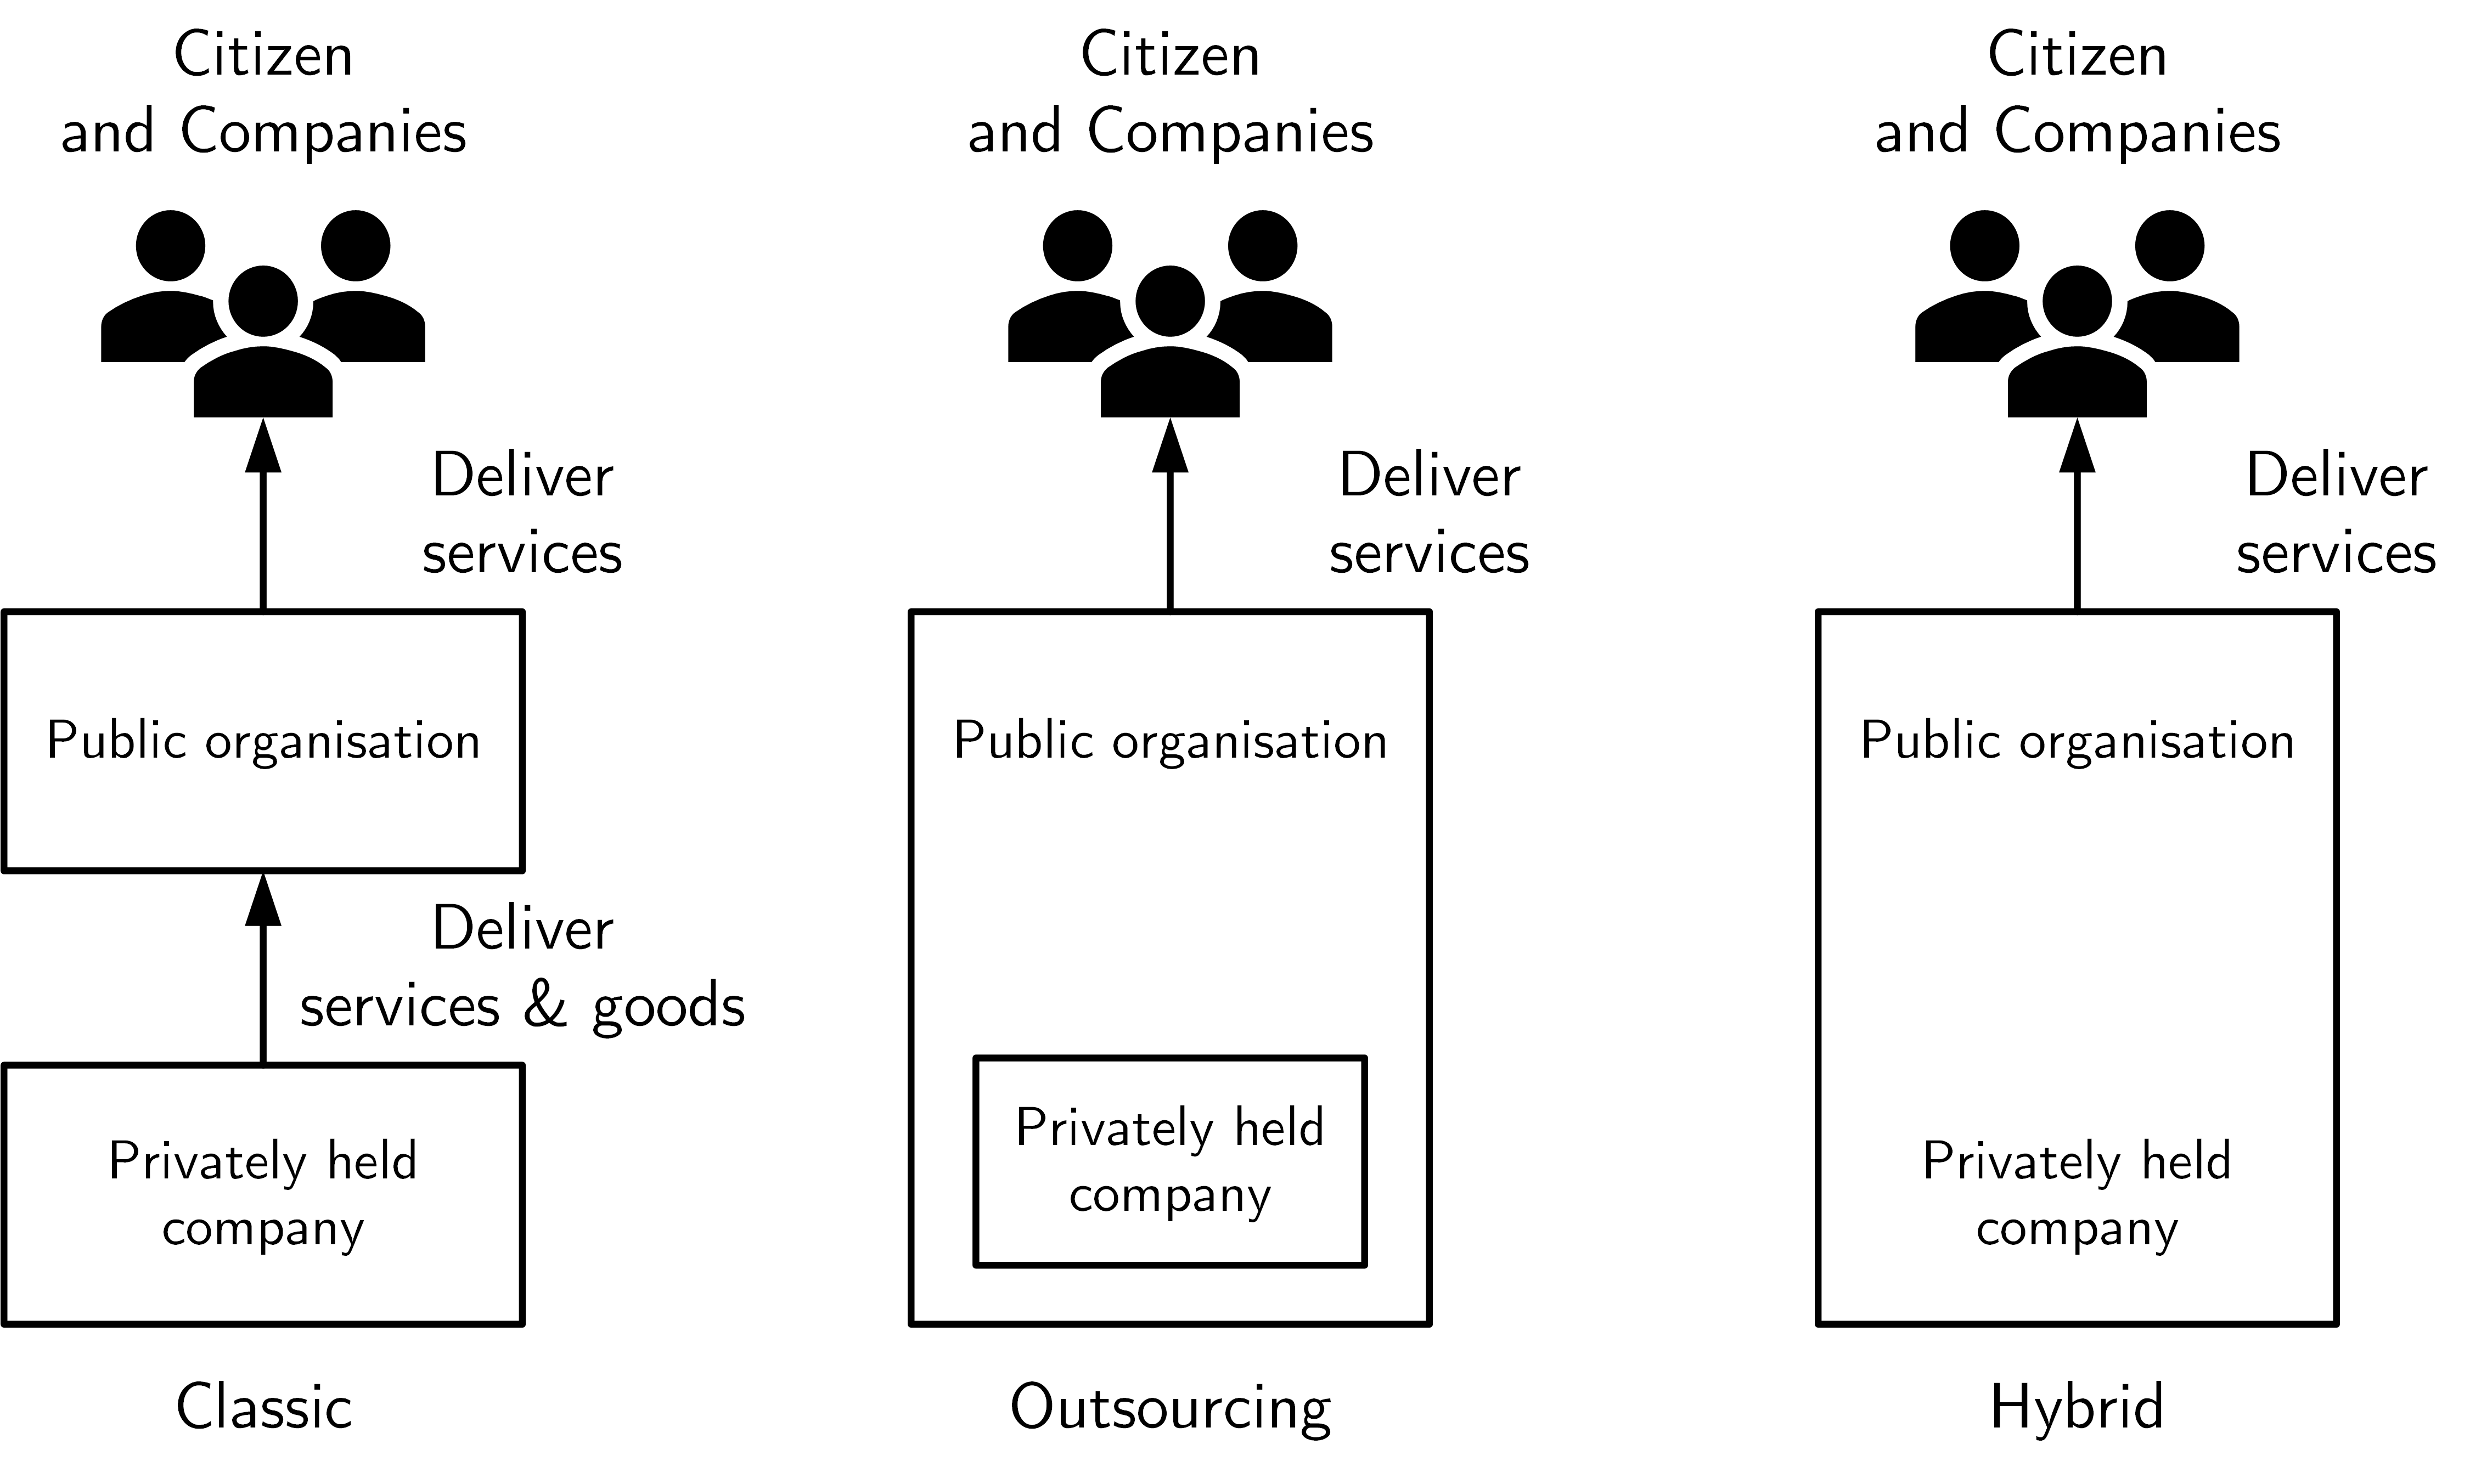
\includegraphics[width=0.7\linewidth]{images/publicsector3modelsofcolaboration}
	\caption[Public sector collaboration models]{Public sector collaboration models}
	\label{fig:publicsector3modelsofcolaboration}
\end{figure}

The public sector is divided into three levels \parencite{PrivacySense2016}:

\begin{itemize}
	\item{\textbf{The national government,} such as the military, the tax authority, and homeland affairs.}
	\item{\textbf{The regional government,} such as the provinces, the police, and water management.}
	\item{\textbf{The local government,} such as the municipalities, the social services, and the local tax offices.}
\end{itemize}

I will focus this research on the public sector level local government of the Netherlands. In \cref{ch:discussion} I will discuss the applicability on non Dutch public sectors.

\section{Introduction of the concept Enterprise Architecture}
\label{introea}
\acrfull{ea} is a discipline for proactively and holistically leading enterprise responses to disruptive forces by identifying and analysing the execution of change toward desired business vision and outcomes. \acrshort{ea} delivers value by presenting business and IT leaders with signature-ready recommendations for adjusting policies and projects to achieve targeted business outcomes that capitalise on relevant business disruptions \parencite{Gartner}.

\textcite{White2018} states that the organisation’s business requirements guide \acrshort{ea} — it helps layout how information, business and technology flow together. \acrshort{ea} has become a priority for businesses trying to keep up with new technologies such as the cloud, \acrfull{iot}, machine learning and other emerging trends that will prompt digital transformation.

IEEE Definition

Concept architectures needed for the problem statement (business, application, information, technology).

\section{Introduction of the concept of antifragility}
\label{sec:introantifragility}
\textcite{Taleb2008} describes a black swan as an event that 1) is so rare that even the possibility that it might occur is unknown, 2) has a catastrophic impact when it does occur, and 3) is explained in hindsight as if it were actually predictable. For extremely rare events, \citeauthor{Taleb2008} argues that the standard tools of probability and prediction, such as the normal distribution, do not apply since they depend on large population and past sample sizes that are never available for rare events by definition. Extrapolating, using statistics based on observations of past events is not helpful for predicting black swans, and might even make us more vulnerable to them. In his book \Gls{antifragile}, \textcite{Taleb2012} states that the way to survive a black swan event is to be \gls{antifragile}.\par
Most people answer that the opposite of \gls{fragile} is \gls{robust}, \gls{resilient}, solid, or something of the sort. However, the \gls{resilient}, \gls{robust} (and company) are items that neither break nor improve, so you would not need to write anything on them — have you ever seen a package with \gls{robust} in thick green letters stamped on it? Logically, the exact opposite of a \gls{fragile} parcel would be a package on which one has written, please mishandle or please handle carelessly. Its contents would not just be unbreakable but would benefit from shocks and a wide array of trauma \parencite{Taleb2012}.

\begin{figure}[h!]
	\centering
	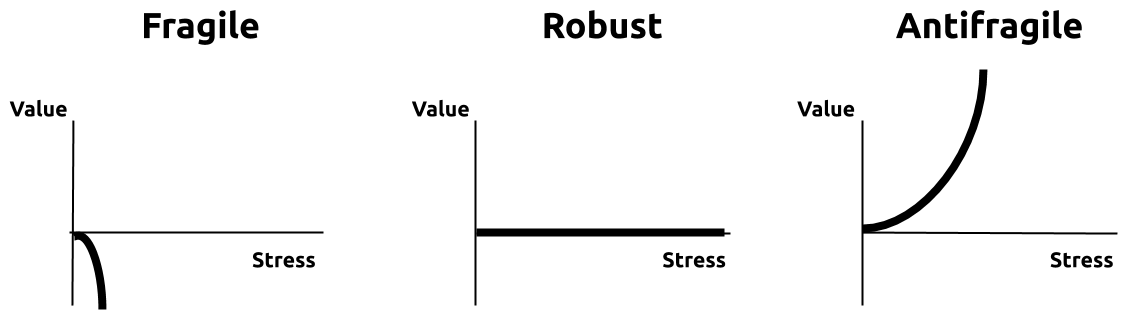
\includegraphics[width=0.7\linewidth]{images/eaal-triad}
	\caption[EAAL Triad]{\acrshort{eaal} Triad \parencite{Botjes2020}}
	\label{fig:eaal-triad}
\end{figure}

\section{Problem statement}
\label{sec:problemstatement}
The concept of \gls{antifragility} implies that organisations could benefit and strengthen from crises, volatility, errors and uncertainty and could also lead to opportunities for innovation \parencite{Kastner2017}. Enterprise Architecture is a discipline that helps organisations to reach their goals. As stated by 

As described in \ref{introea} with \acrshort{ea} one would expect that an organisation uses the discipline of \acrshort{ea} to get more towards the state of \gls{antifragility}. Research has been conducted on aspect architectures such as the application and information architectures but not on \acrshort{ea}. The problem is that the Body of Knowledge contains no direct knowledge on how to achieve \gls{antifragility} with the use of \acrshort{ea}. 

\section{The research subject}
\label{sec:researchsubject}
\acrshort{ea} facilitates an organisation in assessing the impact of change and making recommendations for target states that support business objectives. \acrshort{ea} guides an organisation in changing. \acrshort{ea} can help organisations in changing towards the state of \gls{antifragility}.

As described in \ref{introea} \acrshort{ea} is used to steer an system towards its goals. However, what are the success factors of \acrshort{ea} that contribute in accomplishing \gls{antifragility}? This is summarised in a conceptual research model.
\begin{figure}[H]
	\centering
	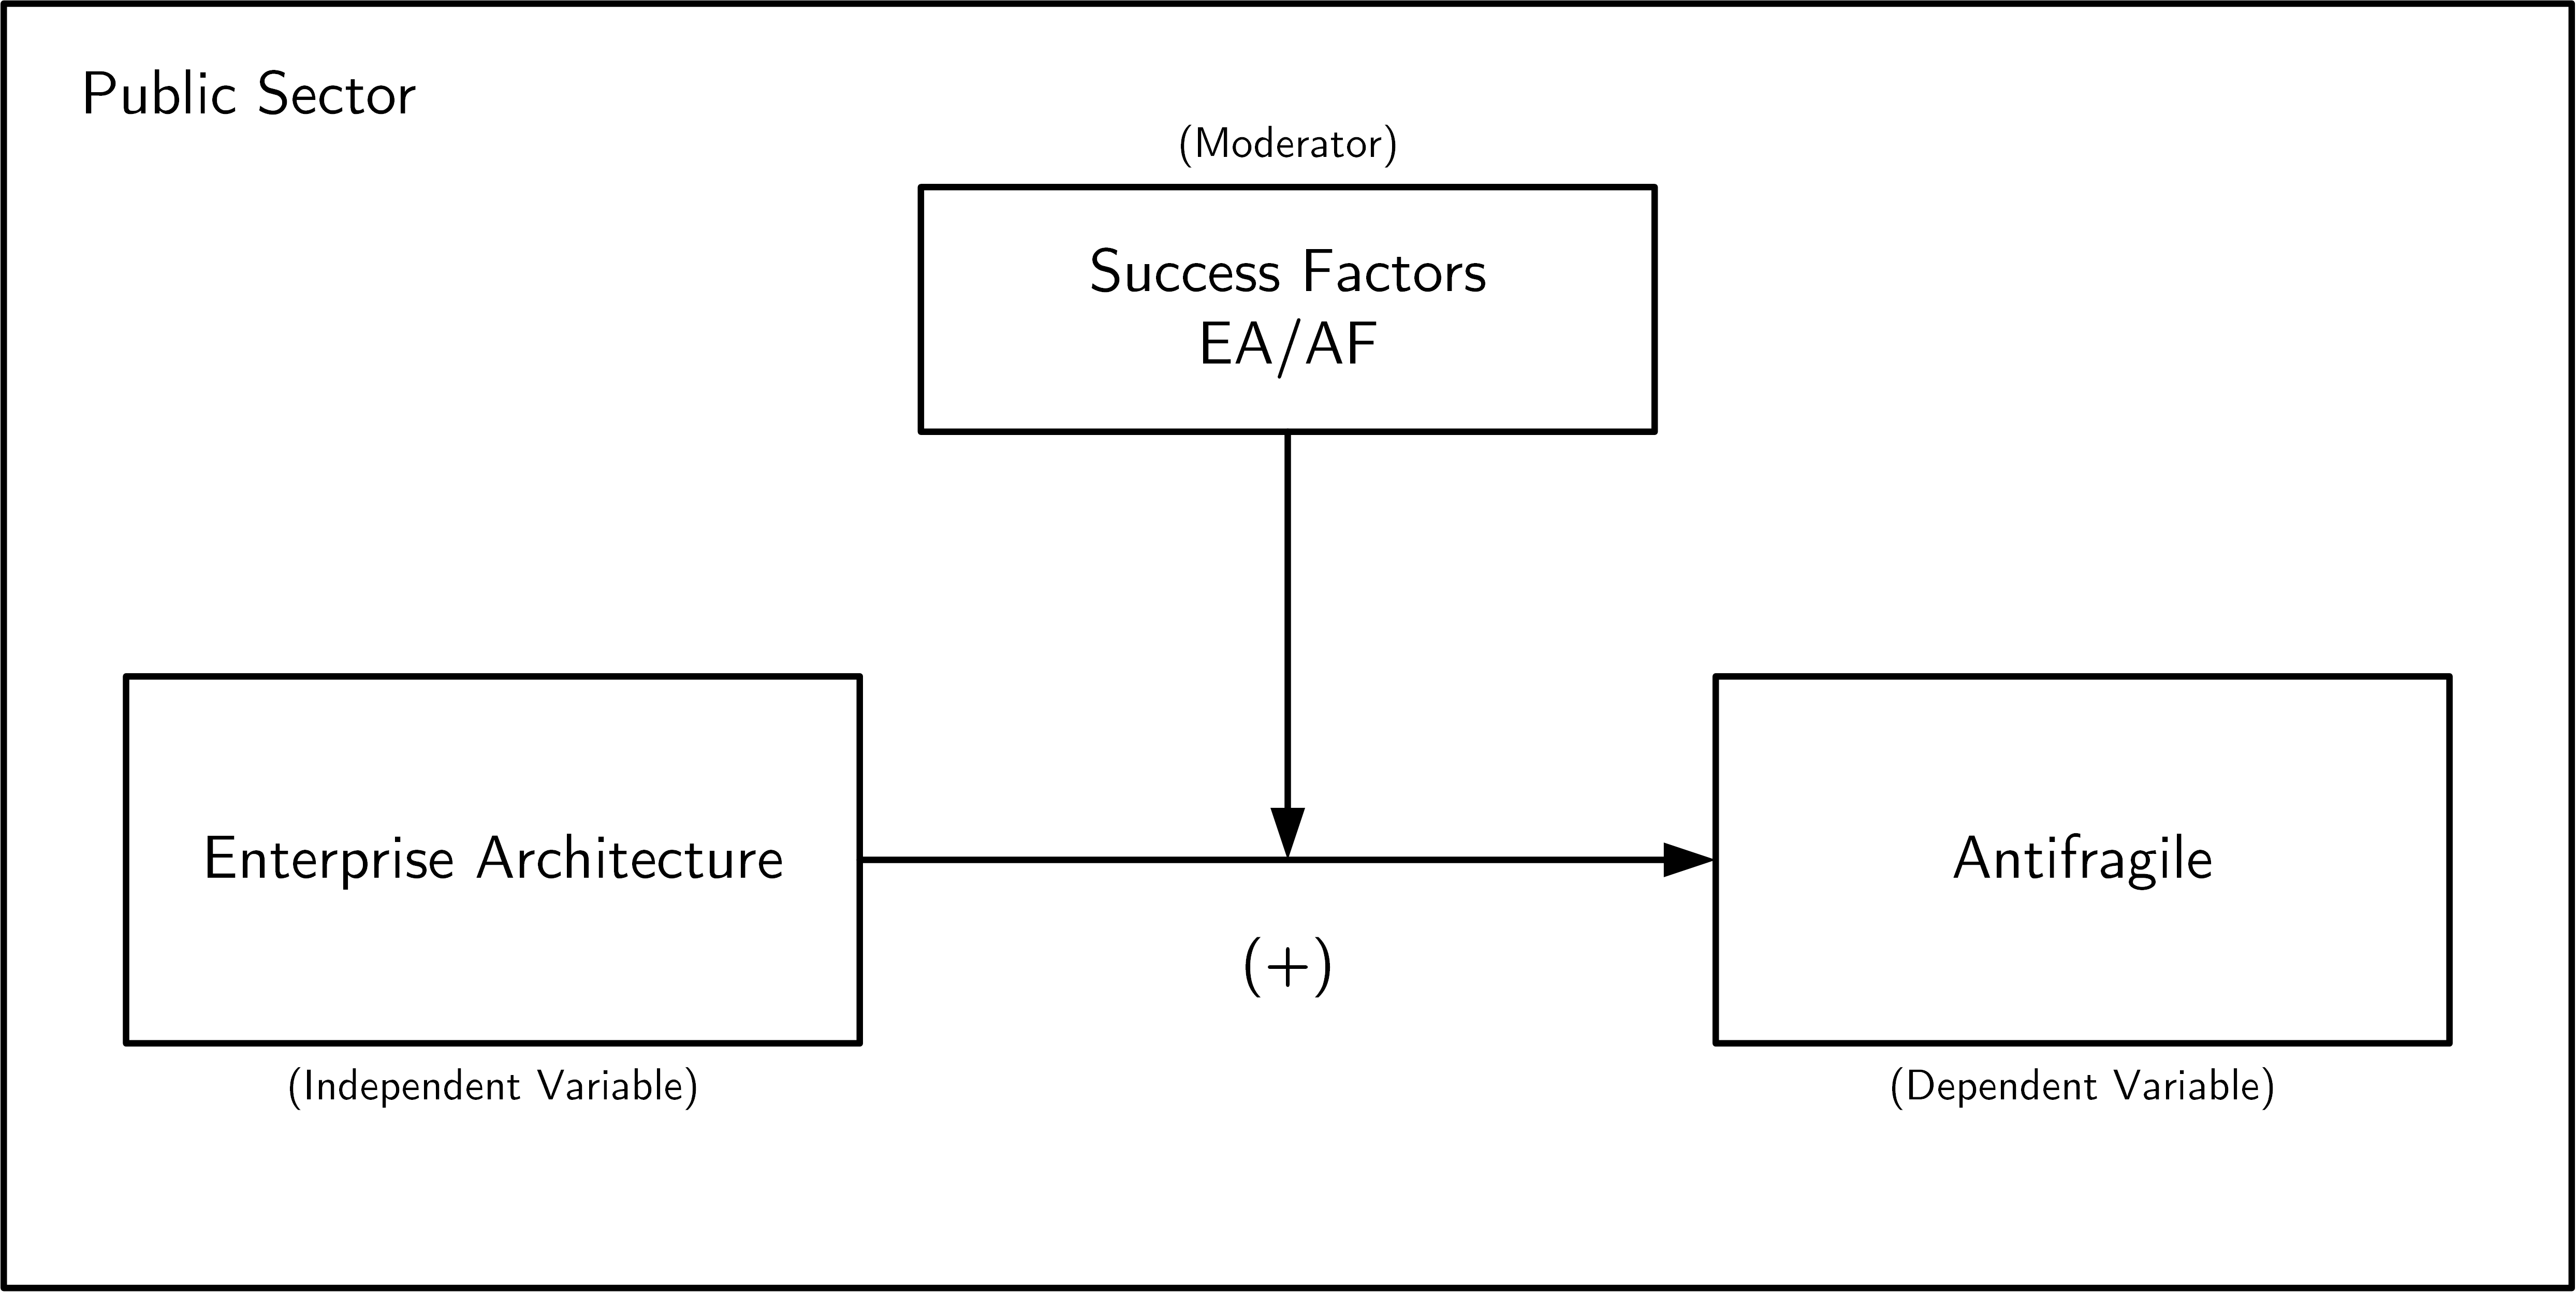
\includegraphics[width=0.8\linewidth]{images/conceptualmodel}
	\caption[Conceptual Research Model]{Conceptual Research Model}
	\label{fig:conceptualmodel}
\end{figure}

The hypothesis of the conceptual research model is that, in the context of the system public sector, \acrlong{ea} success factors have a positive influence in the contribution of \acrlong{ea} in achieving antifragility in that system. From this conceptual research model the research question can be stated as:\bigskip

\noindent \emph{''What are the success factors of \acrlong{ea} for \gls{antifragility} in the public sector?''}\bigskip

\noindent To correctly answer this research question the following sub-questions need to be answered:

\begin{enumerate}
	\item{What is literature saying about the public sector?}
	\item{What is literature saying about \acrlong{ea}?}
	\item{What is literature saying about the success factors of Enterprise Architecture?}
	\item{What does literature say about antifragile?}
%	\item{How can the success factors of \acrlong{ea} contribute to becoming antifragile?}
\end{enumerate}
\section{Research relevance}
\label{sec:researchrelevance}

\acrfull{ea} has contributed to being more \gls{robust}, \gls{resilient}, and \gls{agile}. Using \acrshort{ea} in pursuing \gls{antifragility} will add value to companies by accelerating and growing when there is a stressor or black swan event. The \gls{antifragile} theory is young.  \citeauthor{Taleb2012} published the theory in his book ''\Gls{antifragile}: Things that gain from disorder.'' in \citeyear{Taleb2012}.  Studies conducted on \acrshort{ea} with the concept of \gls{antifragile} are almost non-existence. The conducted studies are primarily about making IT Systems \gls{antifragile}. \textcite{Botjes2020,Kastner2017} are exceptions and have researched how to apply \gls{antifragile} in an organisational context. Nevertheless, both concluded that there is more research needed. The former used the lens of Enterprise Engineering, which is closely related to \acrshort{ea}, together with resilience, while the latter used mostly reslience as its lens. There is still no answer to how \acrshort{ea} can contribute to becoming \gls{antifragile}. Organisations use the practice of \acrshort{ea} to guide them to achieve their goals. Giving more insights on this subject will contribute to the Body of Knowledge and help others getting closer to \gls{antifragility} by using \acrshort{ea}.

\begin{figure}[H]
	\centering
	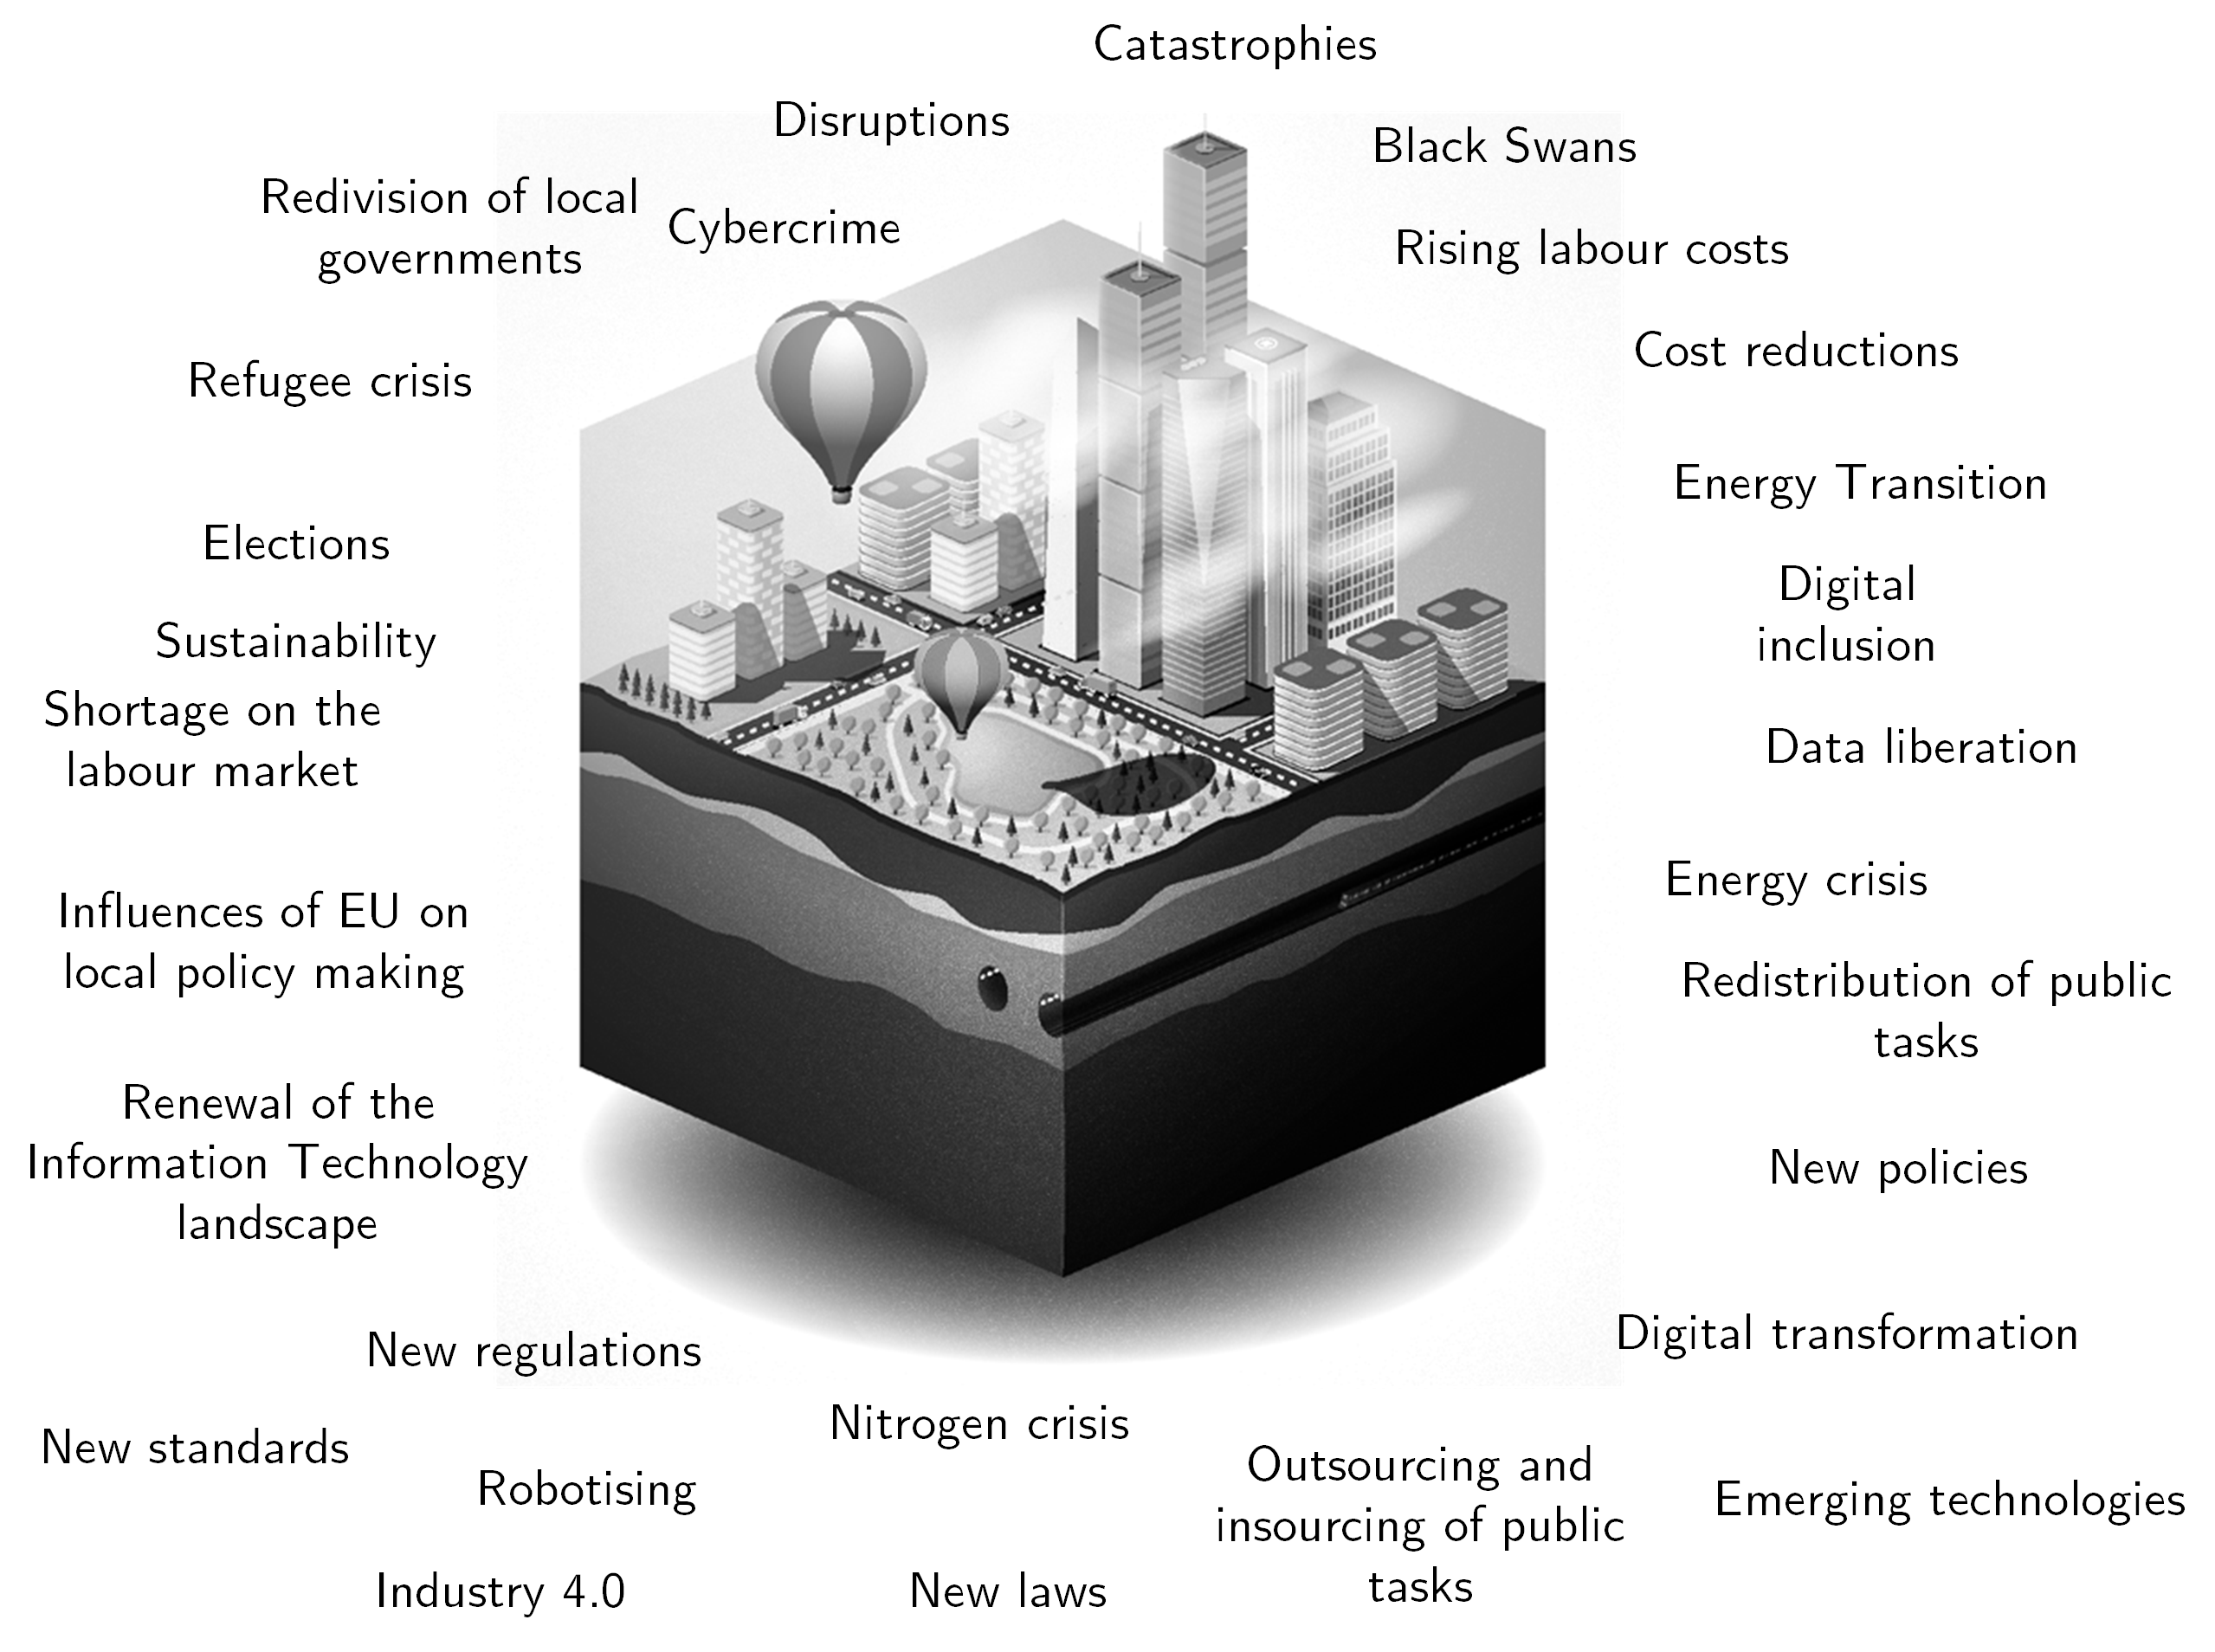
\includegraphics[width=0.8\linewidth]{images/publicstressors}
	\caption[Examples of stressors on the public sector (local governments)]{Examples of stressors on the public sector (local governments)}
	\label{fig:publicstressors}
\end{figure}

Because of the digital transformation, the pace of change is increasing rapidly.  The digital transformation is not the only stressor on the public sector. There are a lot of internal and external stressors. The public sector invested a lot in being less fragile by becoming more agile, robust, and resilient. By being more agile, robust, or resilient, you can only withstand the change or the stressor but you do not gain from it. Governmental agencies and suppliers in the public sector are searching for methods of dealing with this increased pace and the disruptions that occur. The relevance of this research is not only about the addition to the Body of Knowledge but also to share the outcome with the public sector.

 			%	Add the introduction
	\chapter{Background}
\label{ch:theoreticalbackground}
This research uses three main concepts of interest: \textit{the \gls{ps}}, \textit{\gls{antifragile}}, and \textit{\gls{ea}}. Understanding the interpretation of these concepts is essential for a \gls{sharedmentalmodel}. Besides the three main concepts, it is vital to understand the concept system. The three main concepts use \textit{system} as a concept. The concepts \textit{\gls{ps}}, \textit{\gls{antifragile}}, \textit{\gls{ea}}, and \textit{system} are defined for a \gls{sharedmentalmodel}.
\section{System}
\label{sec:tbsystem}
Literature often uses the concept of system but with a different meaning \parencite[p.~37]{Lapalme2012}. System is used for many different things like software applications, interrelated people, systems of numerous interrelated elements (economical, social, technological) and others.

System has various definitions and types. E.g. open and closed, linear and non-linear, dynamic and deterministic systems \parencite{Rickles2007}. A system can be an area of interest \parencite[p.~13]{Mannaert2016}. However, with another definition, a system is an object that is studied in the field \parencite[p.~933]{Rickles2007}. Both definitions are similar. \Textcite[pp.~13--14]{Mannaert2016} acknowledged that the system is not isolated. The system of concern and systems in the environment have interactions. This behaviour is what \textcite[p.~32]{Bertalanffy1968} calls an open system. An open system is a system that exchanges matter with its environment, as where a closed system is considered to be isolated from its environment \parencite[p.~39]{Bertalanffy1968}.

A system is more than the sum of its parts. It is an indivisible whole \parencites[p.~51--69]{Ackoff1964}[p.~664]{Ackoff1973}. A system loses its essential properties when taken apart. The elements of a system can also themselves be systems. Every system can be a part of another system. These systems are also called sub-systems. This managerial idea of systems thinking is to focus on the interactions of the parts rather than their behaviour separately. 

A mental model to understand a system is dependent on specific characteristics of the behaviour of a system. Understanding the behaviour of a system can only be in its environment \parencite[p.~29]{Gharajedaghi2011}. The boundary of a system is defined by the variables that can be influenced or controlled by the actors of that system \parencite[p.~182]{Gharajedaghi2011}. Variables that can not be influenced or controlled but impact the viability of the system are part of the context \parencite[p.~183]{Gharajedaghi2011} or the environment \parencite[p.~13--14]{Mannaert2016}. The \textit{Why they do} and \textit{What they do} of the actors in the environment help with influencing the environment \parencite[p.~33]{Gharajedaghi2011}. To understand the inner workings, ''one needs the ability to see complementary relations in opposing tendencies and to create feasible wholes with infeasible parts'' \parencite[p.~38]{Gharajedaghi2011}. However, the properties of a system are not the properties of its parts but that of the whole \parencites{Ackoff1973}{Gharajedaghi2011}. Because of these properties, actions intended to produce the desired outcome may generate opposite results, resulting in counter-intuitive behaviour \parencite[p.~48]{Gharajedaghi2011}.

The concepts of the \gls{ps}, \gls{ea} and \gls{antifragility} use different \glspl{specialisation} of the concept system. These \glspl{specialisation} are \textit{\gls{sos}}, \textit{\gls{sie}}, and \textit{Ecosystem}.
\subsection{System-of-Systems and System-in-Environment}
\label{sub:tbsysofsys}
A collection of independent systems that are part of a more extensive system has unique capabilities \parencite{INCOSE2018}. The independent systems working together have unique behaviour that they do not have on their own.  A \gls{sos} is composed of multiple systems \parencites{Ackoff1973}{Gharajedaghi2011}. Another variation is that of a \gls{sie}. Using \gls{sie} stresses that a system is part of and should be aware of its environment \parencites{Gharajedaghi2011}{Lapalme2012}{Korhonen2016}{Mannaert2016}. \gls{sie} is a means to enforce environmental learning. With environmental learning, an enterprise adapts its desired goals to be more compatible with its environment \parencite[p.~41]{Lapalme2012}. The definitions of \gls{sos} and \gls{sie} are within the general definition of a system previously defined by \textcites{Ackoff1973}[p.~183]{Gharajedaghi2011}[pp.~13--14]{Mannaert2016}.

\subsection{Ecosystem}
\label{sub:tbecosystem}
The concept of ecosystem originated from the field of ecology. It was firstly defined by \textcite[p.~229]{Tansley1935} \parencite[p.~19]{Rich1988}. ''But the more fundamental conception is, as it seems to me, the whole system (in the sense of physics), including not only the organism-complex but also the whole complex of physical factors in the widest sense'', is the ecosystem as defined by \textcite[p.~299]{Tansley1935}. There are multiple transfers of the ecological ecosystem concept onto additional domains \parencite[p.~3]{Guggenberger2020}. A company must be viewed not as a member of a single industry but as part of a business ecosystem that crosses a variety of industries \parencite[p.~76]{Moore1993}. A business ecosystem is a concept that various businesses form value creation networks together \parencite[p.~3]{Guggenberger2020}. Ecosystems can be described as ''a set of actors with varying degrees of multilateral, non-generic complementarities that are not fully hierarchically controlled'' \parencite[p.~2255]{Jacobides2018}. There are different ways to order kinds of ecosystems. One way is that of dividing ecosystems into five specialisations. Business ecosystem \parencite[p.~76]{Moore1993}, platform ecosystem \parencite[p.~5]{Guggenberger2020}, service ecosystem \parencites{Barros2006}{Papazoglou2006}{Huang2014}, innovation ecosystem \parencites{Iansiti2004}{Carayannis2009}{Gomes2018}, and software ecosystem \parencites{Manikas2013}[p.~5]{Guggenberger2020}.

\section{Antifragile}
\label{sec:tbantifragile}
What is \gls{antifragile}, where did it originate, what can you achieve with it, and why is \gls{antifragile} important? These questions are the first things that come to mind when hearing \gls{antifragile} for the first time.

Publications on the subject of \gls{antifragile} often use \textit{\gls{stressor}} \parencite[p.~32]{Botjes2020}. What is a \textit{\gls{stressor}}? \textcite[p.~23]{Ghasemi2017} defined \textit{\gls{stressor}} based on \textcites{TurnerII2003}{Chrousos2009} as ''When systems are performing effectively, they are in a predetermined condition and conversely when they are not functioning correctly, they are in an unintended state. An unintended condition can be known or unknown. \textit{\Glspl{stressor}} are forces that threaten to transfer a system from an intended to an unintended condition.''

\Gls{antifragile} originated from the domain of risk management. \Gls{antifragile} was coined for the first time by \textcite{Taleb2012} as his answer to \glspl{blackswan}. \Glspl{blackswan} are ''large-scale unpredictable, and rare events of massive consequences'' \parencite[pp.~6--7]{Taleb2012}. The rarer the event, the less manageable, and the less we know about the frequent of its occurrence. The odds of \gls{blackswan} are not computable. ''Given the unattainability of perfect robustness, we need a mechanism by which the system regenerates itself continuously by using, rather than suffering from, random events, unpredictable shocks, \glspl{stressor}, and \gls{volatility}''. With random events \gls{robust} is not good enough. Everything with the most minute vulnerability breaks. \Gls{robustness} cannot just be it, perfect \gls{robustness} is needed not to end up crashing the system.'' \parencite[p.~8]{Taleb2012}. \Gls{fragile} systems fail when exposed to \glspl{stressor} \parencite[p.~21]{Ghasemi2017}. However, \gls{antifragile} systems prosper and improve in response to unpredictability, \gls{volatile}, randomness, chaos and disturbance (\cref{fig:eaal-triad}). \Gls{antifragility} goes beyond \gls{robustness}.
\begin{figure}[H]
	\centering
	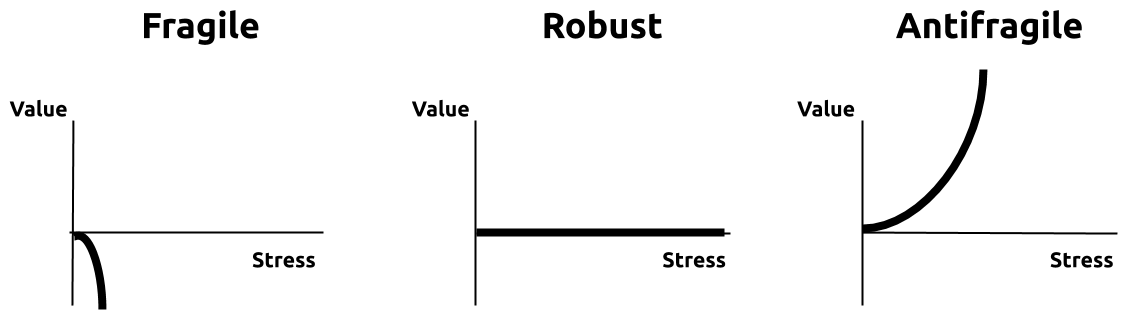
\includegraphics[width=0.8\linewidth]{images/eaal-triad}
	\caption[Triad of fragile, robust, and antifragile \parencite{Botjes2021}]{Triad of fragile, robust, and antifragile \parencite{Botjes2021}}
	\label{fig:eaal-triad}
\end{figure}
\Gls{antifragile} means that a system gains more than it loses. Reducing possible losses will reduce the harmful effects of exposure to damaging elements such as \glspl{stressor} and \gls{blackswan} \parencite[p.~932]{Russo2017}. Positive asymmetry\footnote{Positive asymmetry happens when you have a lot of upside and little downside. Negative asymmetry is when you have little upside and high downside.} is achievable by reducing possible losses. ''\Gls{fragility} and \gls{antifragility} mean potential gain or harm from exposure to something related to \gls{volatility}.'' \parencite[p.~13]{Taleb2012}. That something is what \textcite[p.~13]{Taleb2012} calls a member of the extended disorder family. This disorder family consists of \gls{uncertainty}, variability, imperfect, incomplete knowledge, chance, chaos, \gls{volatility}, disorder, \gls{entropy}, time, the unknown, randomness, turmoil, \glspl{stressor}, error, dispersion of outcomes, unknowledged. The disorder family is interpreted by \textcite[p.~12]{Botjes2020}, based on the works of \textcites[p.~436]{Taleb2012}[p.~3]{Gorgeon2015}, as \acrlong{vuca} from \textcite{Bennis1985}. \Gls{antifragility} is not only an answer to a \gls{blackswan} but also to random events, unpredictable shocks, \glspl{stressor}, and \gls{volatility} \parencite[p.~8]{Taleb2012}.

\subsection{Antifragile as a system property}
\label{sub:backgroundafpropertyofsystem}
A diversity of researchers define that \gls{fragility}, \gls{robustness} and \gls{antifragility} are properties of a system \parencites{Jaaron2014}{Hole2016}{Kastner2017}{OReilly2019}{Botjes2021}. \Gls{selforganisation}, ownership, \gls{diversity}, \glspl{sharedmentalmodel} and a shared vision are some of the properties that an \gls{antifragile} system should posses. \textcite{Botjes2021} conducted extensive research to define \gls{antifragility} and the application of \gls{antifragility} on organisation design. \citeauthor{Botjes2021} used multiple sources (\cref{tab:tbsourcesofantifragileattributes}) to define a list of attributes.
\begin{table}[H]
	\centering
	\begin{tabular}{@{}p{.4\textwidth}p{.4\textwidth}@{}}
		\toprule
		\multicolumn{2}{c}{\textbf{Sources}} \\%
		\midrule
		\textcite{Ghasemi2017} & \textcite{Johnson2013} \\%
		\textcite{Kennon2015} & \textcite{Markey2018} \\%
		\textcite{Hendriksson2016} & \textcite{Kastner2017} \\%
		\textcite{Gorgeon2015} & \textcite{Hole2016} \\%
		\textcite{OReilly2019} & \\%
		\bottomrule
	\end{tabular}%
	\caption[Sources used for antifragile attributes \parencite{Botjes2021}]{Sources used for antifragile attributes \parencite{Botjes2021}}
	\label{tab:tbsourcesofantifragileattributes}%
\end{table}%
The result is the \acrfull{eaal} (\cref{fig:eaalbw}). The \acrfull{eaal} is recent. \textcite[p.~5]{Botjes2021} created the data set through extensive literature research, but the data set only covers literature until June 2019. 
\begin{figure}[H]
	\centering
	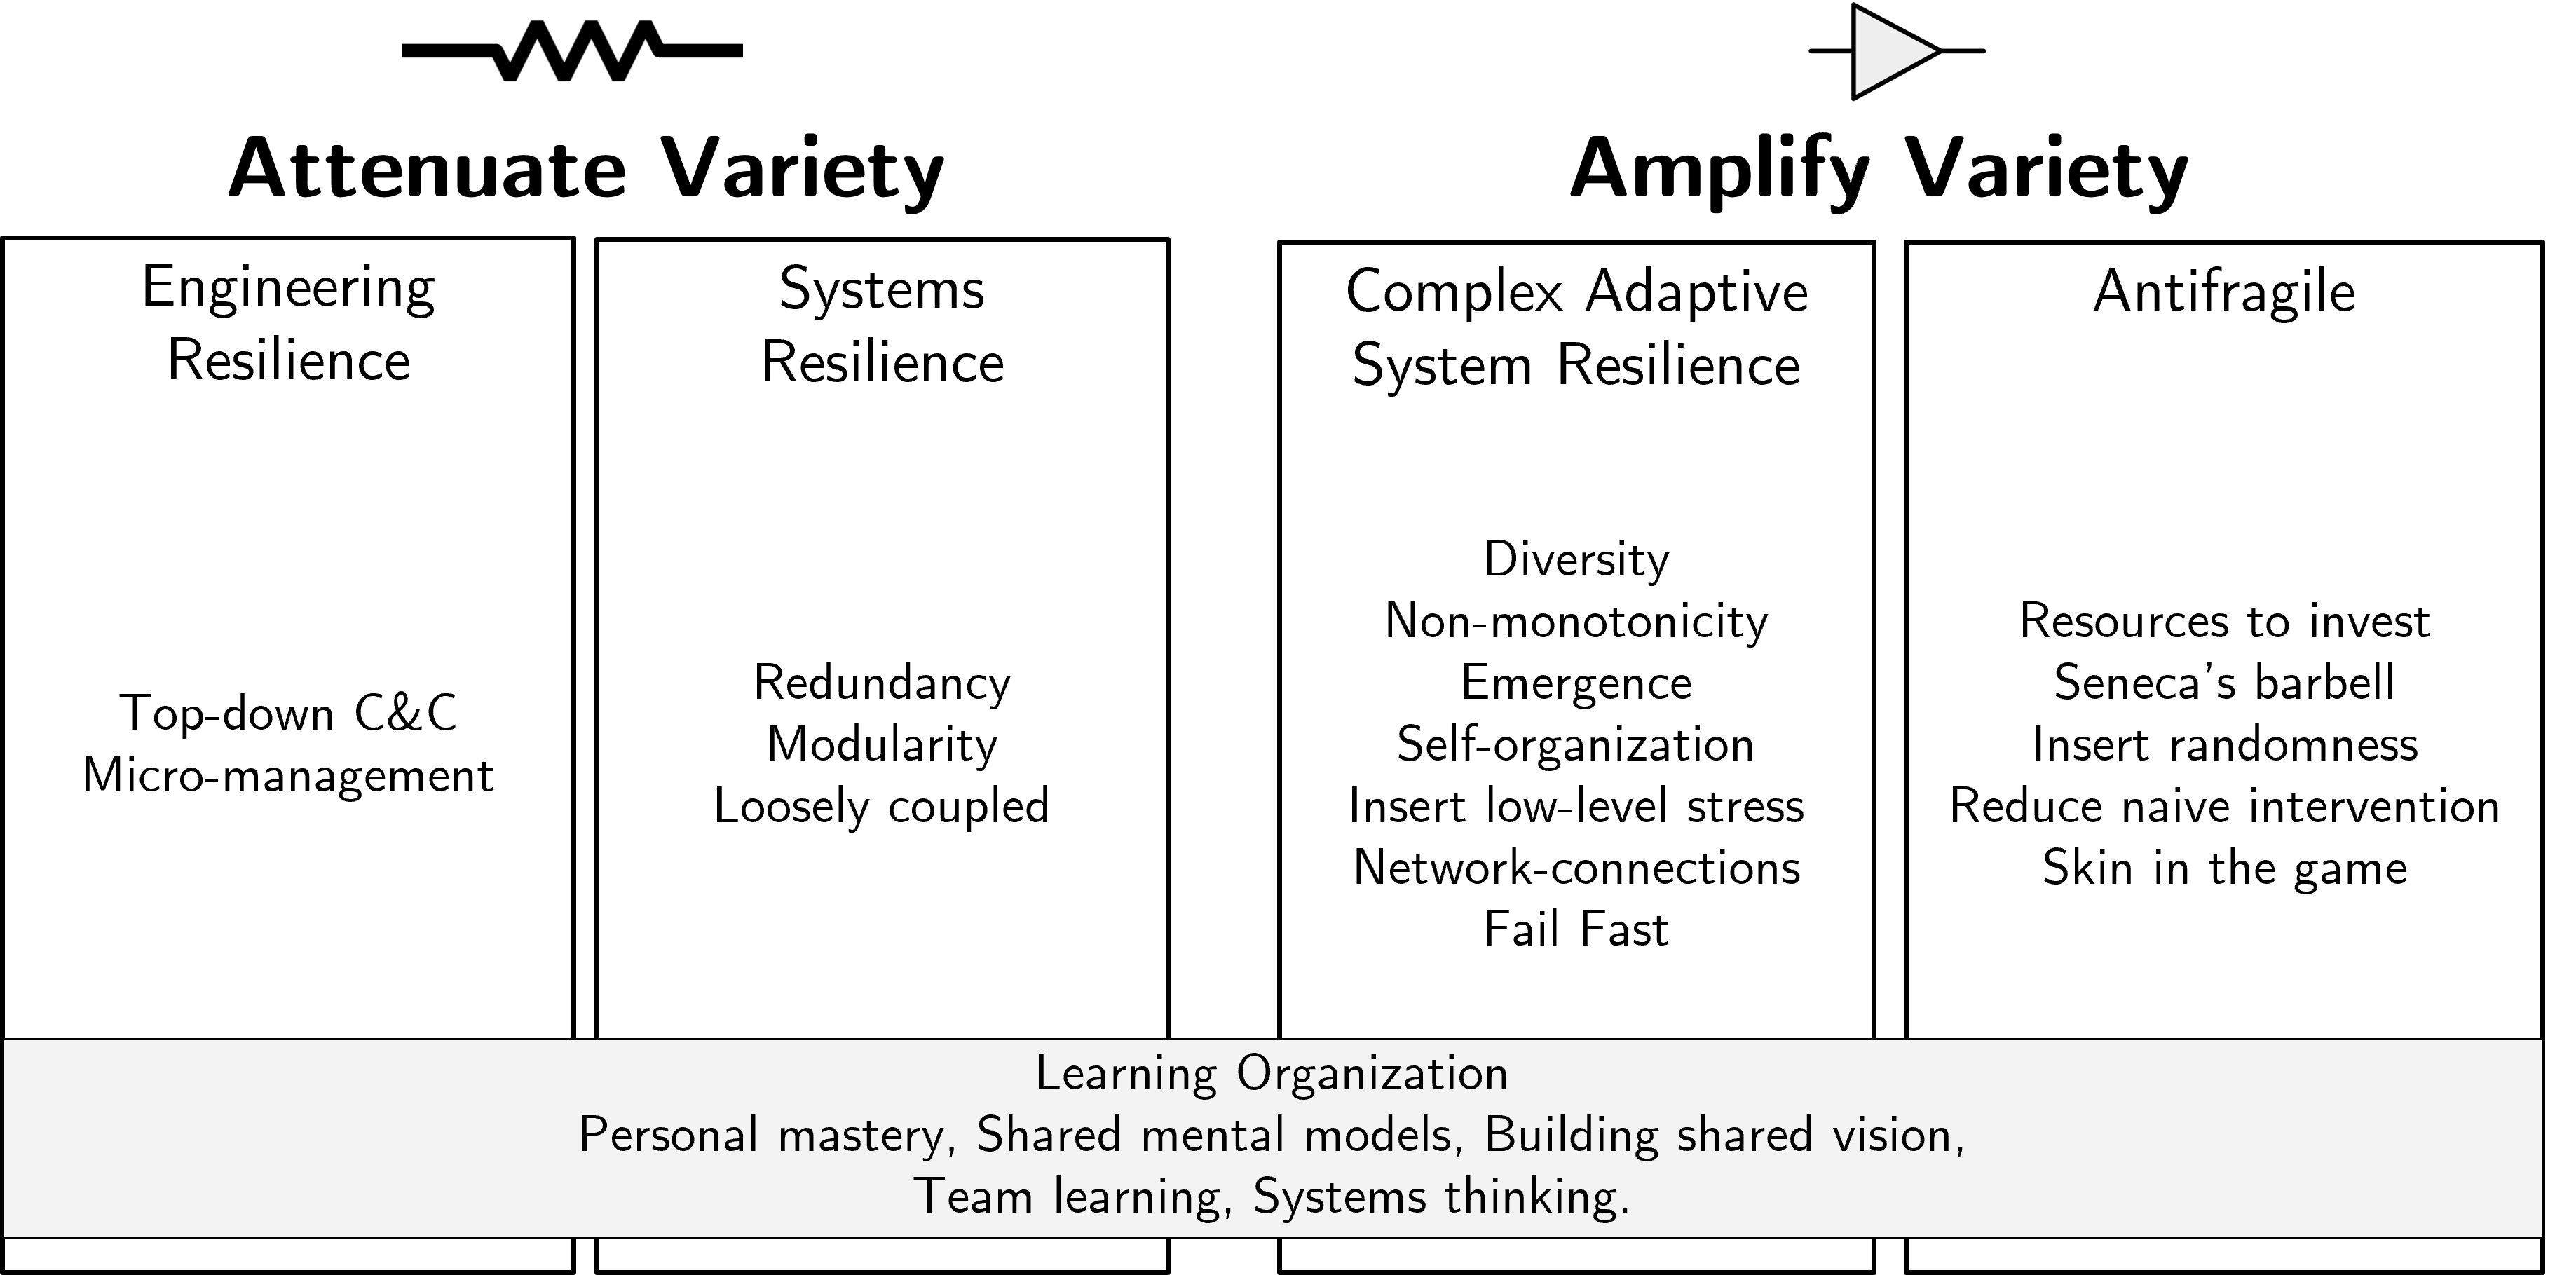
\includegraphics[width=0.8\linewidth]{images/eaalbw}
	\caption[Extended Antifragile Attribute List \parencite{Botjes2021}]{Extended Antifragile Attribute List \Parencite{Botjes2021}}
	\label{fig:eaalbw}
\end{figure}
Searching for \textit{new} literature makes sure that \textcite{Botjes2021} is recent and is not rebutted. Using the time frame of June 2019 until April 2022 makes sure that only new literature is found. We used the same academic search engines and keywords as \textcite[p.~5]{Botjes2021}. The result of the search was \textit{thirty-one} new sources. These sources are new articles, books and in-proceedings (\cref{app:literaturecatchup}). We rated the new findings on accessability, if it was already part of \textcite{Botjes2021}, and if the sources contained information on properties and attributes of \gls{antifragility}. Of those thirty-one new sources, three were already in the literature set of \textcite{Botjes2021}. Eight were not found or publicly available, and thirteen were not relevant. Only seven were of interest to look at. After reading them, none of the literature added something new or rebutted the work of \textcite{Botjes2021}. \textcite{Botjes2021} is recent and contains possible \glspl{attribute} to become more \gls{antifragile} in the Dutch \gls{ps}.

The \acrlong{eaal} (\cref{fig:eaalbw}) classifies \glspl{attribute} in two primary and five secondary categories. \textit{\Gls{attenuatevariety}} and \textit{\gls{amplifyvariety}} (\cref{sub:attenuatevsaplify}) are the two primary categories. The five secondary categories are \textit{\gls{engineeringresilience}}, \textit{\gls{systemsresilience}}, \textit{\gls{casresilience}} (\cref{sub:tbresilience}), \textit{\gls{antifragile}} and \textit{learning organisation} (\cref{sub:learningorganisation}). The \acrlong{eaal} does not contain resilience as a secondary category but multiple types of resilience. The \acrlong{eaal} assigned the secondary categories to the primary categories. \textit{\Gls{engineeringresilience}} and \textit{\gls{systemsresilience}} are assigned to \textit{\gls{attenuatevariety}}, while \textit{\gls{casresilience}} and \textit{\gls{antifragile}} to \textit{\gls{amplifyvariety}}. \textit{Learning organisation} is the only category assigned to both \textit{\gls{attenuatevariety}} and \textit{\gls{amplifyvariety}}.
\subsection{Resilience}
\label{sub:tbresilience}
\Gls{resiliency} is mentioned often in relation to \gls{antifragility}. \textcites[loc.~280]{Kastner2017}[p.~3]{Botjes2021} uses the definitions of \textcite[pp.~5--8]{MartinBreen2011}. \textcite[pp.~5--8]{MartinBreen2011} identified several types of resiliency. These types are  \textit{\gls{engineeringresilience}} (Common Sense resilience), \textit{\gls{systemsresilience}} (Robustness in economics), and \textit{\gls{casresilience}}. The definitions of \gls{resiliency} (\cref{tab:resiliencetypes}) have focus on the avoidance of harmful \glspl{stressor} and failure, including \gls{uncertainty} and \gls{volatility} \parencite[pp.~5--8]{MartinBreen2011}.
\begin{longtable}{p{.3\textwidth}p{.55\textwidth}}
	\toprule%
	\textbf{Type} & \textbf{Description} \\%
	\midrule%
	\endhead%
	\hline
	\endfoot%
	\caption[Types of resilience \parencite{MartinBreen2011}]{Types of resilience \parencite{MartinBreen2011}}
	\label{tab:resiliencetypes}
	\endlastfoot%
	\Gls{engineeringresilience} & Bounce back faster after stress, enduring greater stresses, and being disturbed less by a given amount of stress. \\%
	\Gls{systemsresilience} & Maintaining system function in the event of a disturbance. Systems resilience has been applied in governance and management, where it is often called robustness. \\%
	\Gls{casresilience} & The ability to withstand, recover from, and reorganise in repsonse to crisis. The function is maintained by the system structure may not be. The main differentiator is the adaptive capacity or adaptability of the system.\\%
	\bottomrule%
\end{longtable}
\subsection{Learning organisation}
\label{sub:learningorganisation}
One of the secondary categories of \acrlong{eaal} is learning organisation. But what is the learning organisation? The learning organisation is a way to create resilient organisations. These resilient organisations can cope better with unknown and unpredictable evens. ''Continuous improvement requires commitment to learning.'' \parencite{Garvin1993}. The learning organisation is an organisation that is equipped for creating, acquiring, and transferring knowledge \parencite{Garvin1993}. The result of this is that a learning organisation can modify its behaviour to reflect new knowledge and insights \parencite{Garvin1993}. \textcite{Senge1994} defined the \glspl{attribute} of the learning organisation that \textcite{Botjes2021} used in the \acrlong{eaal} (\cref{fig:fithdiscipline}). These attributes are \textit{\gls{personalmastery}}, \textit{\glspl{sharedmentalmodel}}, \textit{\gls{buildingsharedvision}}, \textit{\gls{teamlearning}}, and \textit{\gls{systemsthinking}}.
\begin{figure}[H]
	\centering
	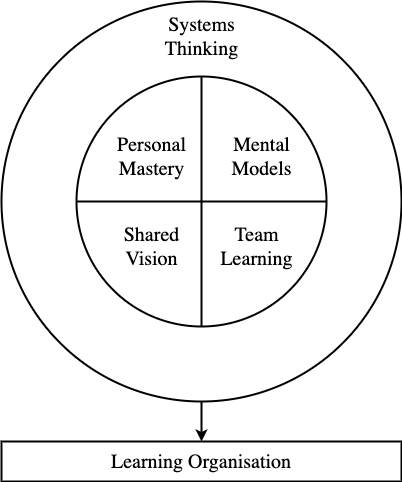
\includegraphics[width=0.4\linewidth]{images/fithdiscipline}
	\caption[The Fifth discipline \parencite{Senge1994}]{The Fifth discipline \parencite{Senge1994}}
	\label{fig:fithdiscipline}
\end{figure}

\subsection{Attenuate variety and amplified variety}
\label{sub:attenuatevsaplify}
The two main categories in the \acrlong{eaal} are \gls{attenuatevariety} and \gls{amplifyvariety}. What is \gls{attenuatevariety} and \gls{amplifyvariety}? Variety originated from Cybernetics and was coined by \textcite{Ashby1956}. Variety denotes the count of states of a system. \citeauthor{Ashby1956} and \citeauthor{Beer1979} stated the Law of Requisite Variety as 'variety can destroy variety ' \parencite[p.~207]{Ashby1956} and 'variety absorbs variety' \parencite[p.~286]{Beer1979}. ''If a system is to be stable, the number of states of its control mechanism must be greater than or equal to the number of states in the system being controlled.'' \parencite{Heylighen2001}. There are two types of variety manipulations \parencites{Ashby1956}{Beer1979}. \Gls{attenuatevariety} is reducing the variety in a system, while \gls{amplifyvariety} is increasing the variety in a system. ''To amplify internal variety is about increasing the chance of a higher \gls{entropy} and, therefore, more capable of absorbing the increasing external variety caused by change.'' \parencite[p.~4]{Botjes2021}. \Gls{attenuatevariety} is about increasing the chance of a lower \gls{entropy} and, therefore, less capable of absorbing increasing external variety caused by change. \Gls{engineeringresilience} and \gls{systemsresilience} are results from \gls{attenuatevariety}, while \gls{casresilience} and \gls{antifragile} of \gls{amplifyvariety}. Another interpretation is possible. \Gls{attenuatevariety} increases the \gls{fragility} of a system, while \gls{amplifyvariety} decreases the \gls{fragility} and increases the \gls{antifragility} of a system.
\subsection{Is agility antifragility?}
\label{tb:antifragile_vs_agility}
In the introduction on \gls{antifragility} (\cref{sec:introantifragility}) we mentioned that \textcite[pp.~79--81]{Steen2018} recognised \gls{fragility}, \gls{robustness}, \gls{resiliency}, \gls{agility}, and \gls{antifragility} as manifestations of \textcite{Taleb2012}. Nevertheless, \gls{agility} is not used, or in some cases mentioned, by \textcites{Taleb2012}{Kastner2017}{OReilly2019}{Botjes2021} and others.

What is the relation between \gls{agile} and \gls{antifragile}? Is \gls{agile} \gls{fragile}, \gls{robust} or \gls{antifragile}? The question is \gls{agile} \gls{fragile}, \gls{robust} or \gls{antifragile} is improperly framed \parencite[p.~6]{Tomov2019}. \Gls{agility} can be \gls{fragile}, \gls{robust} or \gls{antifragile}. \Gls{antifragility} and \gls{robustness} are mathematically defined as properties, while \gls{agility} is not. Rather than aiming to control or remove control, we have to build technical and business systems that aim to be \gls{antifragile} to change \parencite[p.~884]{OReilly2019}. When we architect \gls{antifragility}, businesses can gain \gls{agility}. When we build systems that aim to be \gls{antifragile} for change is better than to control change. The result is the possibility of creating business and technical architectures that enable \gls{agility} through design.

Based on experiences and observations, five trademarks and twenty-three practices are defined for organisational agility \parencite[p.~7]{Aghina2018}. When we combine these trademarks and practices with the \acrlong{eaal} from \textcite[p.~7]{Botjes2021} it is clear that by using the attributes from the \acrlong{eaal} it is possible to achieve \gls{agility} in a system. \Gls{agility} can be the result of applying \gls{antifragile} \glspl{attribute}. \Gls{agility} is a result of implementation, while \gls{antifragile} is a property of a system.
\subsection{Antifragile system attributes}
\label{sub:attributesofantifragile}
The \acrlong{eaal} is selected as a source and starting point for \gls{antifragile} attributes (\cref{sub:backgroundafpropertyofsystem}). \Gls{optionality} is stated as an essential attribute by \textcites{Taleb2012}[p.~64]{Botjes2020}. \Gls{optionality} is excluded from the \acrlong{eaal} because of the overlap with \gls{diversity} \parencite[p.~64]{Botjes2020}. But \textcites{Taleb2012}[p.~9]{Gorgeon2015} both use the term \gls{optionality}. \Gls{optionality} is an idea advanced by \textcite{Taleb2012}. At the most basic level, \gls{optionality} means having lots of options. The difference between \gls{optionality} and \gls{diversity} is very subtle. \Gls{optionality} allows the buyer to retain the upper bound and be unaffected by adverse outcomes which makes the buyer \gls{antifragile} \parencite{Cunff2020}. Despite the minimal difference between \gls{optionality} and \gls{diversity}, \gls{optionality} can still have a distinctive character in the Dutch \gls{ps}. Adding \gls{optionality} to the already defined set of the \acrlong{eaal} brings a total of twenty-three attributes. The \acrlong{eaal} categorised the attributes into \gls{attenuatevariety}, \gls{amplifyvariety}, and \gls{learningorganisation}. Adding \gls{optionality} to \gls{amplifyvariety} makes it equal to \gls{diversity}. For the overview of the \glspl{attribute} for \gls{antifragile} see \cref{tab:attributesofantifragile}. 
\begin{longtable}{@{}p{.4\textwidth}p{.4\textwidth}@{}}
	\toprule%
	\textbf{Attribute} & \textbf{Category} \\%
	\midrule%
	\endhead%
	\hline
	\endfoot%
	\caption[Antifragile system attributes]{Antifragile system attributes}
	\label{tab:attributesofantifragile}
	\endlastfoot%
	\Gls{topdowncc} & \Gls{attenuatevariety} \\%
	\Gls{micromanagement} & \Gls{attenuatevariety} \\%
	\Gls{redundancy} & \Gls{attenuatevariety} \\%
	\Gls{modularity} & \Gls{attenuatevariety} \\%
	\Gls{looselycoupled} & \Gls{attenuatevariety} \\%
	\Gls{diversity} & \Gls{amplifyvariety} \\%
	\Gls{nonmonotonicity} & \Gls{amplifyvariety} \\%
	\Gls{emergence} & \Gls{amplifyvariety} \\%
	\Gls{selforganisation} & \Gls{amplifyvariety} \\%
	\Gls{insertlowlevelstress} & \Gls{amplifyvariety} \\%
	\Gls{networkconnections}  & \Gls{amplifyvariety} \\%
	\Gls{failfast} & \Gls{amplifyvariety} \\%
	\Gls{resourcestoinvest} & \Gls{amplifyvariety} \\%
	\Gls{senecabarbell} & \Gls{amplifyvariety} \\%
	\Gls{insertrandomness} & \Gls{amplifyvariety} \\%
	\Gls{reducenaiveintervention} & \Gls{amplifyvariety} \\%
	\Gls{skininthegame} & \Gls{amplifyvariety} \\%
	\Gls{optionality} &  \Gls{amplifyvariety} \\%
	\Gls{personalmastery} &  \Gls{learningorganisation} \\%
	\Gls{sharedmentalmodel} &  \Gls{learningorganisation} \\%
	\Gls{buildingsharedvision} &  \Gls{learningorganisation} \\%
	\Gls{teamlearning} &  \Gls{learningorganisation} \\%
	\Gls{systemsthinking} &  \Gls{learningorganisation} \\%
	\bottomrule%
\end{longtable}

\section{Public sector}
\label{sec:tbpublicsector}
The context of this research is the public sector. We need to explain the Dutch \gls{ps} to have a common understanding that will help to place this research in its proper context. However, we will not explain how the Dutch \gls{ps} functions in depth.

In general the \gls{ps} is the collective name for all government and semi-government organisations \parencite[p.~261]{Pathirane1982}. We divide the governments into three levels: the national government, the regional government, and the local government. We see these levels also in the Dutch \gls{ps}: the central government, the provinces, and the municipalities \parencite[p.~10]{Libert2016}. The Netherlands is a decentralised unitary state. A decentralised unitary state is a form of government in which territorial units within a unitary state have independent powers \parencite[p.~8]{Engels2013}. The organisation of local and regional authorities is formalised in the Netherlands by the Provinces Act and the Municipalities Act. Provinces and municipalities can therefore decide on issues themselves. There is no fixed demarcation of tasks between the levels of the government. Nevertheless, provinces and municipalities have a general power to regulate and manage, which can only be limited by law. However, provinces and municipalities are obliged to cooperate in implementing rules set by higher authorities.

My observation is that, as a result, there are differences in the implementation of laws between municipalities themselves. E.g. one municipality is helping residents get financially healthier by coaching, while another municipality is employing them. In both cases it is about a law for social benefits performed by municipalities. In theory you can have \underline{n} different implementations of the law with \underline{n} being the number of municipalities.

The central government is the part of the government that works at the national level \parencite{Rijksoverheid2019}. They are responsible for policy-making, passing laws and monitoring compliance. In addition, the central government is responsible for preparing plans for the government and parliament and carrying out these plans.  The provinces can decide independently on many matters. E.g. the creation of new nature and building new roads. In addition, the provinces also implement several national laws. Municipalities only perform tasks that are of direct importance to their residents. Making those choices is the essential task of a municipal council. In addition, the municipalities also implement many national laws. For example, every municipality must issue passports and identity cards to its residents. 

As of 2022, the national government consists of 12 ministries \parencite{Linthorst2021}, the regional government of 12 provinces \parencite{CBS2022prov}, and the local government of 344 municipalities \parencite{CBS2022prov}. Organisations that are part of the public sector but are not classified as an organisation belonging to one of the three levels are excluded from this count. 

A difference between the public sector and other sectors is public accountability. Public accountability is a form of accountability that relates specifically to the public sector \parencite{Boers2009}. Public accountability should be distinguished from public responsibilities, which involve a substantive discussion about the public sector's tasks, obligations, and liabilities. Public accountability relates to public funds' expenditure and the exercise of public duties and powers. It is transparent for the public, and it is from the public good perspective. You see this also when you compare the public and private sectors on core values. Public accountability is the most important value in the public sector, while profitability is almost non-existing \parencite[p.~472]{Wal2008}. The top five public sector core values are accountability, effectiveness, incorruptibility, reliability, and lawfulness.

\subsection{The public sector as a system}
\label{sub:tbpssystemofsystems}
In general, the Dutch \gls{ps} is the collective name for all government and semi-government organisations \parencite[p.~261]{Pathirane1982}. Besides the central government, provinces, and municipalities, we also have semi-government organisations that are part of the public sector. An organisation is part of the semi-government if the government finances it, performs public tasks, and serves a public good. Examples of semi-government organisations are the organisations of public transportation, healthcare, and education. When we use the theory of systems (\cref{sec:tbsystem}) we can say that the public sector is a System of Systems. But is it correct that the sub-systems are only government and semi-government organisations?

The \gls{ps} is working closely together with the private sector in so-called Public-Private Partnerships. A Public-Private Partnership is when the government and the industry work together to realise a project based on a clear division of tasks and risks \parencite[p.~8]{Enneman2007}. While at the same time retaining their own identities and responsibilities. A Public-Private Partnership realises added value---a qualitative better product for the same investment or the same quality for a lower investment. Besides the Public-Private Partnership, you see also other forms of collaboration. Like collaborations in innovations. ''By working together with private companies and start-ups and learning from each other, we will develop new innovative solutions \parencite[p.~120]{Digitaleoverheid2021}. ''We can also give others the space to innovate public services, for example, by releasing open data (under conditions) so that large and small companies can develop so-called 'gov tech' solutions. The government does not always have to do this innovation itself or have it commissioned.'' \parencite[p.~120]{Digitaleoverheid2021}. "Only through cooperation within the government and the business community, education and science can we strengthen technological developments." \parencite[p.~68]{Digitaleoverheid2021}.

The role of private sector organisations is changing more and more. \Glspl{jv} are formed between public and private sector organisations in stead of private sector organisations only delivering products and services to the \gls{ps}. Can the Dutch \gls{ps} reach its goal of being more responsive and adaptive to respond more adequately and flexible to unforeseen circumstances without the private sector? We have the opinion that they cannot. There are many dependencies and there is a high interconnectedness (coherency). We decided to place the private sector organisations working with the Dutch \gls{ps} in the \gls{sos} of the Dutch \gls{ps} (\cref{fig:pssystemofsystems}).
\begin{figure}[H]
	\centering
	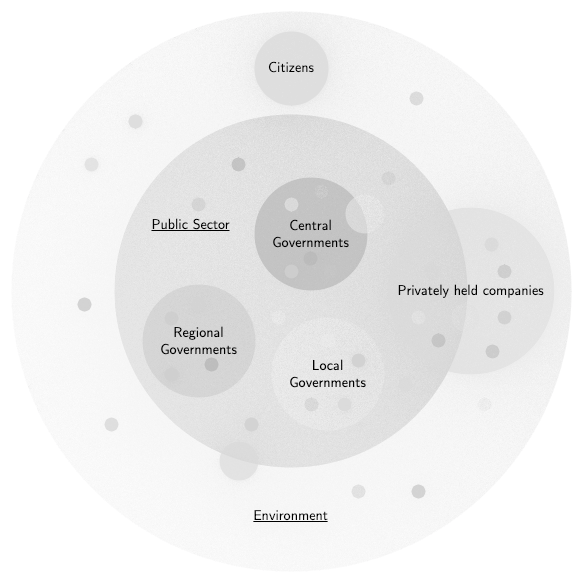
\includegraphics[width=0.6\linewidth]{images/pssystemofsystems}
	\caption[Public Sector as a \gls{sos}]{Public Sector as a \gls{sos}}
	\label{fig:pssystemofsystems}
\end{figure}

\section{Enterprise Architecture}
\label{sec:tbenterprisearchitecture}
This research is about which success factors positively influence \gls{ea} in achieving \gls{antifragility} in the Dutch \gls{ps}. This statement already assumes that \gls{ea} is a means to achieve a goal. Is this correct? Does the world have the same idea about \gls{ea}, or do they see it differently? Can \gls{ea} contribute to reaching the goals of an organisation or even a system? Regardless of the attention \gls{ea} gets, many researchers and practitioners have indicated that there is a lack of a shared mental model \parencite[p.~2]{SaintLouis2019}. The various definitions are not always complimentary, and sometimes they are even opposite \parencites{Dietz2008}{Hoogervorst2009}{Lapalme2012}{SaintLouis2019}. ''Unfortunately, the term ''Enterprise Architecture'' has many meanings as well, meanings that are quite diverse and sometimes even contradictory.'' \parencite[p.~51]{Dietz2008}. A lens on Enterprise Architecture needs to be defined for this research to create a shared understanding of Enterprise Architecture. There is no shared mental model of Enterprise Architecture \parencite[p.~2]{SaintLouis2019}. The lack of a shared mental model can create confusion and conflicts concerning the purpose of Enterprise Architecture and its practice \parencite[p.~1]{SaintLouis2019}. The definitions vary in the scope of application. Some definitions only focus on \acrlong{it} systems, while others focus on the business, the enterprise, the environment, or any other combination. E.g. the definitions from \textcites{Gartner}{Dietz2008}{Graves2009}{Ross2014}{White2018}.
\vskip\baselineskip
\noindent \underline{Definition of \textcite{Gartner}}: \gls{ea} analyses the execution of change toward a desired business vision and outcomes. \gls{ea} leads the enterprise proactively and holistically, responding to disruptive forces.
\vskip\baselineskip
\noindent \underline{Definition of \textcite[p.~53]{Dietz2008}}: Theoretical, architecture is the normative restriction of design freedom. Practically, architecture is a consistent and coherent set of design principles.
\vskip\baselineskip
\noindent \underline{Definition of \textcite[pp.~4--5]{Graves2009}}: \gls{ea} is a discipline through which an Enterprise can identify, develop and manage its knowledge of its purpose, its structure and itself. \gls{ea} will also assist in managing changes imposed on the organisation by the market, by regulations, or -- at an operations level -- by system failures, environmental incidents or customer complaints.
\vskip\baselineskip
\noindent \underline{Definition of \textcite[p.~9]{Ross2014}}: \gls{ea} is the organising logic for business processes and IT infrastructure, reflecting its operating model's integration and standardisation requirements. It provides a long term view of a company's processes, systems and technologies so that individuals can build capabilities and not just fulfil immediate needs.
\vskip\baselineskip
\noindent \underline{Definition of \textcite{White2018}}: \gls{ea} is the process by which organizations standardize and organize IT infrastructure to aligns with business goals. These strategies support digital transformation, IT growth and the modernization of IT as a department. \gls{ea} is the practice of analysing, designing, planning and implementing enterprise analysis to successfully execute on business strategies. \gls{ea} helps to lay out how information, business and technology flow together.
\vskip\baselineskip
Four out of five definitions are mostly about deterministic blueprinting. The only definition that is different is that of \textcite{Dietz2008}. The definition of \textcite{Dietz2008} is more about emerging architecture. We also see another difference. With the first four definitions the outcome of the architecture is often the architecture product itself while with \textcite{Dietz2008} the ''architecture is not what you see but what shaped what you see.''. All five \gls{ea} definitions provide decision-support for direction and change at any level of the enterprise. E.g. ''The choices in the journey of an enterprise for an executive, the preferred technologies or process models for new developments for programme and portfolio management, as well planning when to decommission, change or replace systems'' \parencite[p.~4]{Graves2009}. The real difference between the definitions is that the definition of \textcite{Dietz2008} only limits the design freedom by defining boundaries while the other definitions are more deterministic and intended. Because a shared mental model is absent, there is also no clear approach to practising \gls{ea} \parencite[p.~2]{SaintLouis2019}.
\subsection{Approaches of Enterprise Architecture}
\label{sub:eaapproaches}
There are several perspectives on the practice of \gls{ea} \parencites{Lapalme2012}{Kotusev2015}{Ylinen2018}{Ylinen2020}. One of the perspectives is an approach that distinguishes two groups of \gls{ea} experts. A modelling-focused group forms a comprehensive view of an organisation, and a development-focused group using \gls{ea} for organisational development \parencites[p.~6]{Ylinen2020}. 

However, another perspective distinguished three approaches \parencite[p.~4071]{Kotusev2015}. The traditional \parencite{Spewak1993}, the \acrfull{mit} \parencite{Ross2014}, and the \acrfull{dya} \parencite{Wagter2005} approach \parencite[pp.~4071--4072]{Kotusev2015} (\cref{tab:tbthreeapproaches}).
\begin{longtable}{p{.4\textwidth}p{.6\textwidth}}
	\toprule%
	\textbf{Approach} & \textbf{Description} \\%
	\midrule%
	\endhead%
	\hline
	\endfoot%
	\caption[Three approaches to Enterprise Architecture \parencite{Kotusev2015}]{Three approaches to Enterprise Architecture \parencite{Kotusev2015}}
	\label{tab:tbthreeapproaches}
	\endlastfoot%
	Traditional & A four-step sequential process. Document the current (as-is, baseline) state, develop the desired future (to-be, future) state and the transition plan to migrate from the current to the target state, and implement the plan and repeat the process. \\%
	\acrshort{mit} & Advocates the development of a long-term enterprise-level architectural vision to be translated into concrete project-level decisions through IT governance mechanisms. These decisions involve business and IT managers on different organisational levels. \\%
	\acrshort{dya} & ''Just enough, just in time'' architecture. The development of \gls{ea} starts no earlier than there is a need for it. Business initiatives trigger the activities of 
	\gls{ea} to make sure that needed projects fit nicely into the existing \gls{ea} and in the strategic plans of the enterprise. \\%
	\bottomrule%
\end{longtable}
When you scrutinise the definitions of the three approaches, it becomes clear that the approaches are focused on organisations and not the environment. The \gls{ea} three schools of thought from \textcite{Lapalme2012} gives another perspective. Three possible schools of thought in the practice of \gls{ea} are, \gls{enterpriseitarchitecting}, \gls{enterpriseintegrating}, and \gls{enterpriseecologicaladaptation} \parencite[pp.~38--41]{Lapalme2012} (\cref{tab:tbschoolsofthought,app:easchoolsproperties}).
\begin{longtable}{p{.4\textwidth}p{.6\textwidth}}
	\toprule%
	\textbf{Approach} & \textbf{Description} \\%
	\midrule%
	\endhead%
	\hline
	\endfoot%
	\caption[Enterprise Architecture schools of thought \parencite{Lapalme2012}]{Enterprise Architecture schools of thought \parencite{Lapalme2012}}
	\label{tab:tbschoolsofthought}
	\endlastfoot%
	\gls{enterpriseitarchitecting} & \gls{ea} is the glue between business and IT. \gls{ea} is an enabler for executing the business strategy. This school is about aligning an enterprise's IT assets to execute business strategy effectively and various operations using the proper IT capabilities. The school \gls{enterpriseitarchitecting} focuses on the \acrlong{it} capabilities while not questioning the business capabilities. \\%
	\gls{enterpriseintegrating} & \gls{enterpriseintegrating} links strategy and execution. It is not only enabling enterprise strategy it also implements it. Designing all the organisational dimensions is fostered with systems thinking. \gls{enterpriseintegrating} is aware of its environment and tries to manage the environment. \\%
	\gls{enterpriseecologicaladaptation} & \gls{ea} fosters organisational learning by designing all facets of the enterprise. It changes the environment and systematically designs the enterprise, including its relationship to the environment. The enterprise's relationship to its environment is an indisputably connected facet. This school of thought enables innovation and \gls{sie} adaptation. It looks for bidirectional incoherence between the enterprise and its environment. Nevertheless, it is the means for organisational innovation and sustainability. It is about enterprise and environment co-evolution. \\%
	\bottomrule%
\end{longtable}
\subsection{Defining a lens on Enterprise Architecture}
\label{sub:definingea}
\Gls{antifragile} deals with \glspl{stressor} and \glspl{blackswan} originating from the (environment of the) system of interest. The \acrlong{eaal} of \textcite{Botjes2021} fosters \gls{organisationallearning} and \gls{systemsthinking} capabilities to deal with \glspl{stressor} and \glspl{blackswan} \parencite[pp.~2--4]{Botjes2021}. Exploring the \gls{ea} schools of thought \parencite{Lapalme2012} makes it clear that \textit{\gls{enterpriseecologicaladaptation}} is probably the best school in the context of \gls{antifragility}. \textit{\gls{enterpriseecologicaladaptation}} has a clear focus on the environment, fosters organisational and \gls{environmentallearning}, and embraces \gls{systemsthinking} \parencite[pp.~40--41]{Lapalme2012}. Although the school \textit{\gls{enterpriseintegrating}} already has the notion of the environment, it is not changing the environment like the school \textit{\gls{enterpriseecologicaladaptation}}. At the same time, \textit{\gls{enterpriseitarchitecting}} has its main focus on the IT organisation of the enterprise itself. If an organisation want to survive in the turbulence of today's markets, the organisation must learn to adapt and innovate \parencite[p.~42]{Lapalme2012}. The school \textit{\gls{enterpriseecologicaladaptation}} is about adapt and innovate.

It is still necessary to define the lens we use on \gls{ea}. The lens on \gls{ea} is partly defined. \textit{'The how'} is known. The \gls{ea} school of thought \gls{enterpriseecologicaladaptation} is selected. The properties of this school are known (\cref{sec:propeea}). We still miss the definition of \gls{ea}. \textit{'The what'} that we will use as a lens. \textcite[p~42]{Lapalme2012} mapped \gls{ea} authors and literature to the three schools of thought (\cref{app:easchoolsresearchers}).
\begin{table}[H]
	\centering
	\resizebox{\textwidth}{!}{%
	\begin{tabular}{p{0.4\textwidth}p{0.6\textwidth}}
		\toprule
		\textbf{Author(s)} & \textbf{Description} \\%
		\midrule
		\citeauthor{Gharajedaghi2011} & \textcite{Gharajedaghi2011}  is about systems theories and does not have its focus on \gls{ea}. \\%
		\citeauthor{Hoogervorst2009} & \textcite{Hoogervorst2009} is about Enterprise Governance and Enterprise Engineering. It addresses \gls{ea} and provides definitions. \gls{ea} is more a design discipline.  \\%
		\citeauthor{Graves2008} & \textcite{Graves2008} is about \gls{ea}, the goal and use of \gls{ea}, and it contains definitions of \gls{ea}. \\%
		\citeauthor{Martin1995} & \textcite{Martin1995}  is about aligning enterprise engineering to people, techology, and strategy. \gls{ea} is more a design discipline. \\%
		\citeauthor{Smith2011} & \textcite{Smith2011} is about an \gls{ea} framework. It does not contain definitions on \gls{ea}. \\%
		\citeauthor{Lapalme2012b} & \textcite{Lapalme2012b}  is not publicly available and accessible. It is about socio-technical systems strengthen \gls{ea}. \\%
		\bottomrule
	\end{tabular}
	}%
	\caption[Authors of Enterprise Ecological Adaptation \parencite{Lapalme2012}]{Authors of Enterprise Ecological Adaptation \parencite{Lapalme2012}}
	\label{tab:eeaauthors}
\end{table}
A lens on \gls{ea} must be aligned with the \gls{ea} school of thought of \gls{enterpriseecologicaladaptation}. But the definition should also support the Dutch \gls{ps} in being more adequate and flexible to unforeseen circumstances, and so \gls{antifragile}. Using the list of authors and sources for the school of thought of \gls{enterpriseecologicaladaptation} (\cref{tab:eeaauthors}) shows that two sources contain definitions of \gls{ea}. The first source that contains a definition is \textcite{Hoogervorst2009}. \textcite[p.~8]{Hoogervorst2009} defines \gls{ea} as something that provides normative guidance for design in order for the enterprise to operate satisfied. \gls{ea} comprises four sets of architecture business, organisation, information, and technology.

The second is that of \textcite{Graves2008}. ''\gls{ea} is the integration of everything the enterprise is and does.'' \parencite[p.~1]{Graves2008}. \gls{ea} is about the structure of the whole of the enterprise—the whole rather than a single sub-system. There are no simple states of 'as is' and 'to be'. The world is dynamic and not static. Everything in a business system depends on everything else \parencite[p.~14]{Graves2008}.

\citeauthor{Graves2008}'s definition directly relates to the \gls{ea} school of thought of \gls{enterpriseecologicaladaptation} and hints towards \gls{antifragility}. But its \gls{ea} is still mostly normative and deterministic. When we compare this with the definition of \gls{ea} from \textcite{Dietz2008} is the definition of \citeauthor{Dietz2008} more emergent. It will adapt easier to unforeseen circumstances. The definition of \textcite{Dietz2008} has a downside. It can be too conceptual to use it correctly but ''it seems to be the only feasible way of ‘translating’ high-level statements, as can be found in mission and strategy documents, into operationally useful principles for the development of systems.'' \parencite[p.~53]{Dietz2008}. We decided to adopt the definition of \textcite{Dietz2008} as our lens.

\subsection{Enterprise Architecture system attributes}
\label{sub:attributesonea}
The \gls{ea} school of thought of Enterprise Ecological Adaptation has the best alignment with \gls{antifragile} (\cref{sec:tbenterprisearchitecture}). The \glspl{attribute} used for \gls{ea} will be those of the school of \gls{enterpriseecologicaladaptation}.  It contains \glspl{attribute} related to learning and \gls{systemsthinking}. \textit{\Gls{organisationallearning}}, \textit{\gls{environmentallearning}}, and \textit{\gls{systeminenvironmentcoevolutionlearning}} are related to learning and \textit{\gls{systeminenvironment}}, \textit{\gls{holisticsystemicstance}}, and \textit{\gls{intraorganisationalcoherency}} to \gls{systemsthinking}. See for a full overview \cref{tab:attributesofeea}.
\begin{longtable}{@{}p{.475\textwidth}p{.475\textwidth}@{}}
	\toprule%
	\textbf{Attribute} & \textbf{Category} \\%
	\midrule%
	\endhead%
	\hline
	\endfoot%
	\caption[Enterprise Architecture system attributes based on \parencite{Lapalme2012}]{Enterprise Architecture system attributes based on \parencite{Lapalme2012}}
	\label{tab:attributesofeea}
	\endlastfoot%
	\Gls{systeminenvironment} & \Gls{enterpriseecologicaladaptation} \\%
	\Gls{holisticsystemicstance} & \Gls{enterpriseecologicaladaptation} \\%
	\Gls{intraorganisationalcoherency} & \Gls{enterpriseecologicaladaptation} \\%
	\Gls{organisationallearning} & \Gls{enterpriseecologicaladaptation} \\%
	\Gls{environmentallearning} & \Gls{enterpriseecologicaladaptation} \\%
	\Gls{systeminenvironmentcoevolutionlearning} & \Gls{enterpriseecologicaladaptation} \\%
	\bottomrule%
\end{longtable} 				%	Add the Theoretical Background
	\chapter{Research Methodology}
\label{ch:research-methodology}

\section{Research Model}
\label{sec:research-model}
The method of \textcite{Verschuren2016} is used for the research model. This method gives me a step-by-step plan for the research.
	\begin{figure}[h]
		\centering
		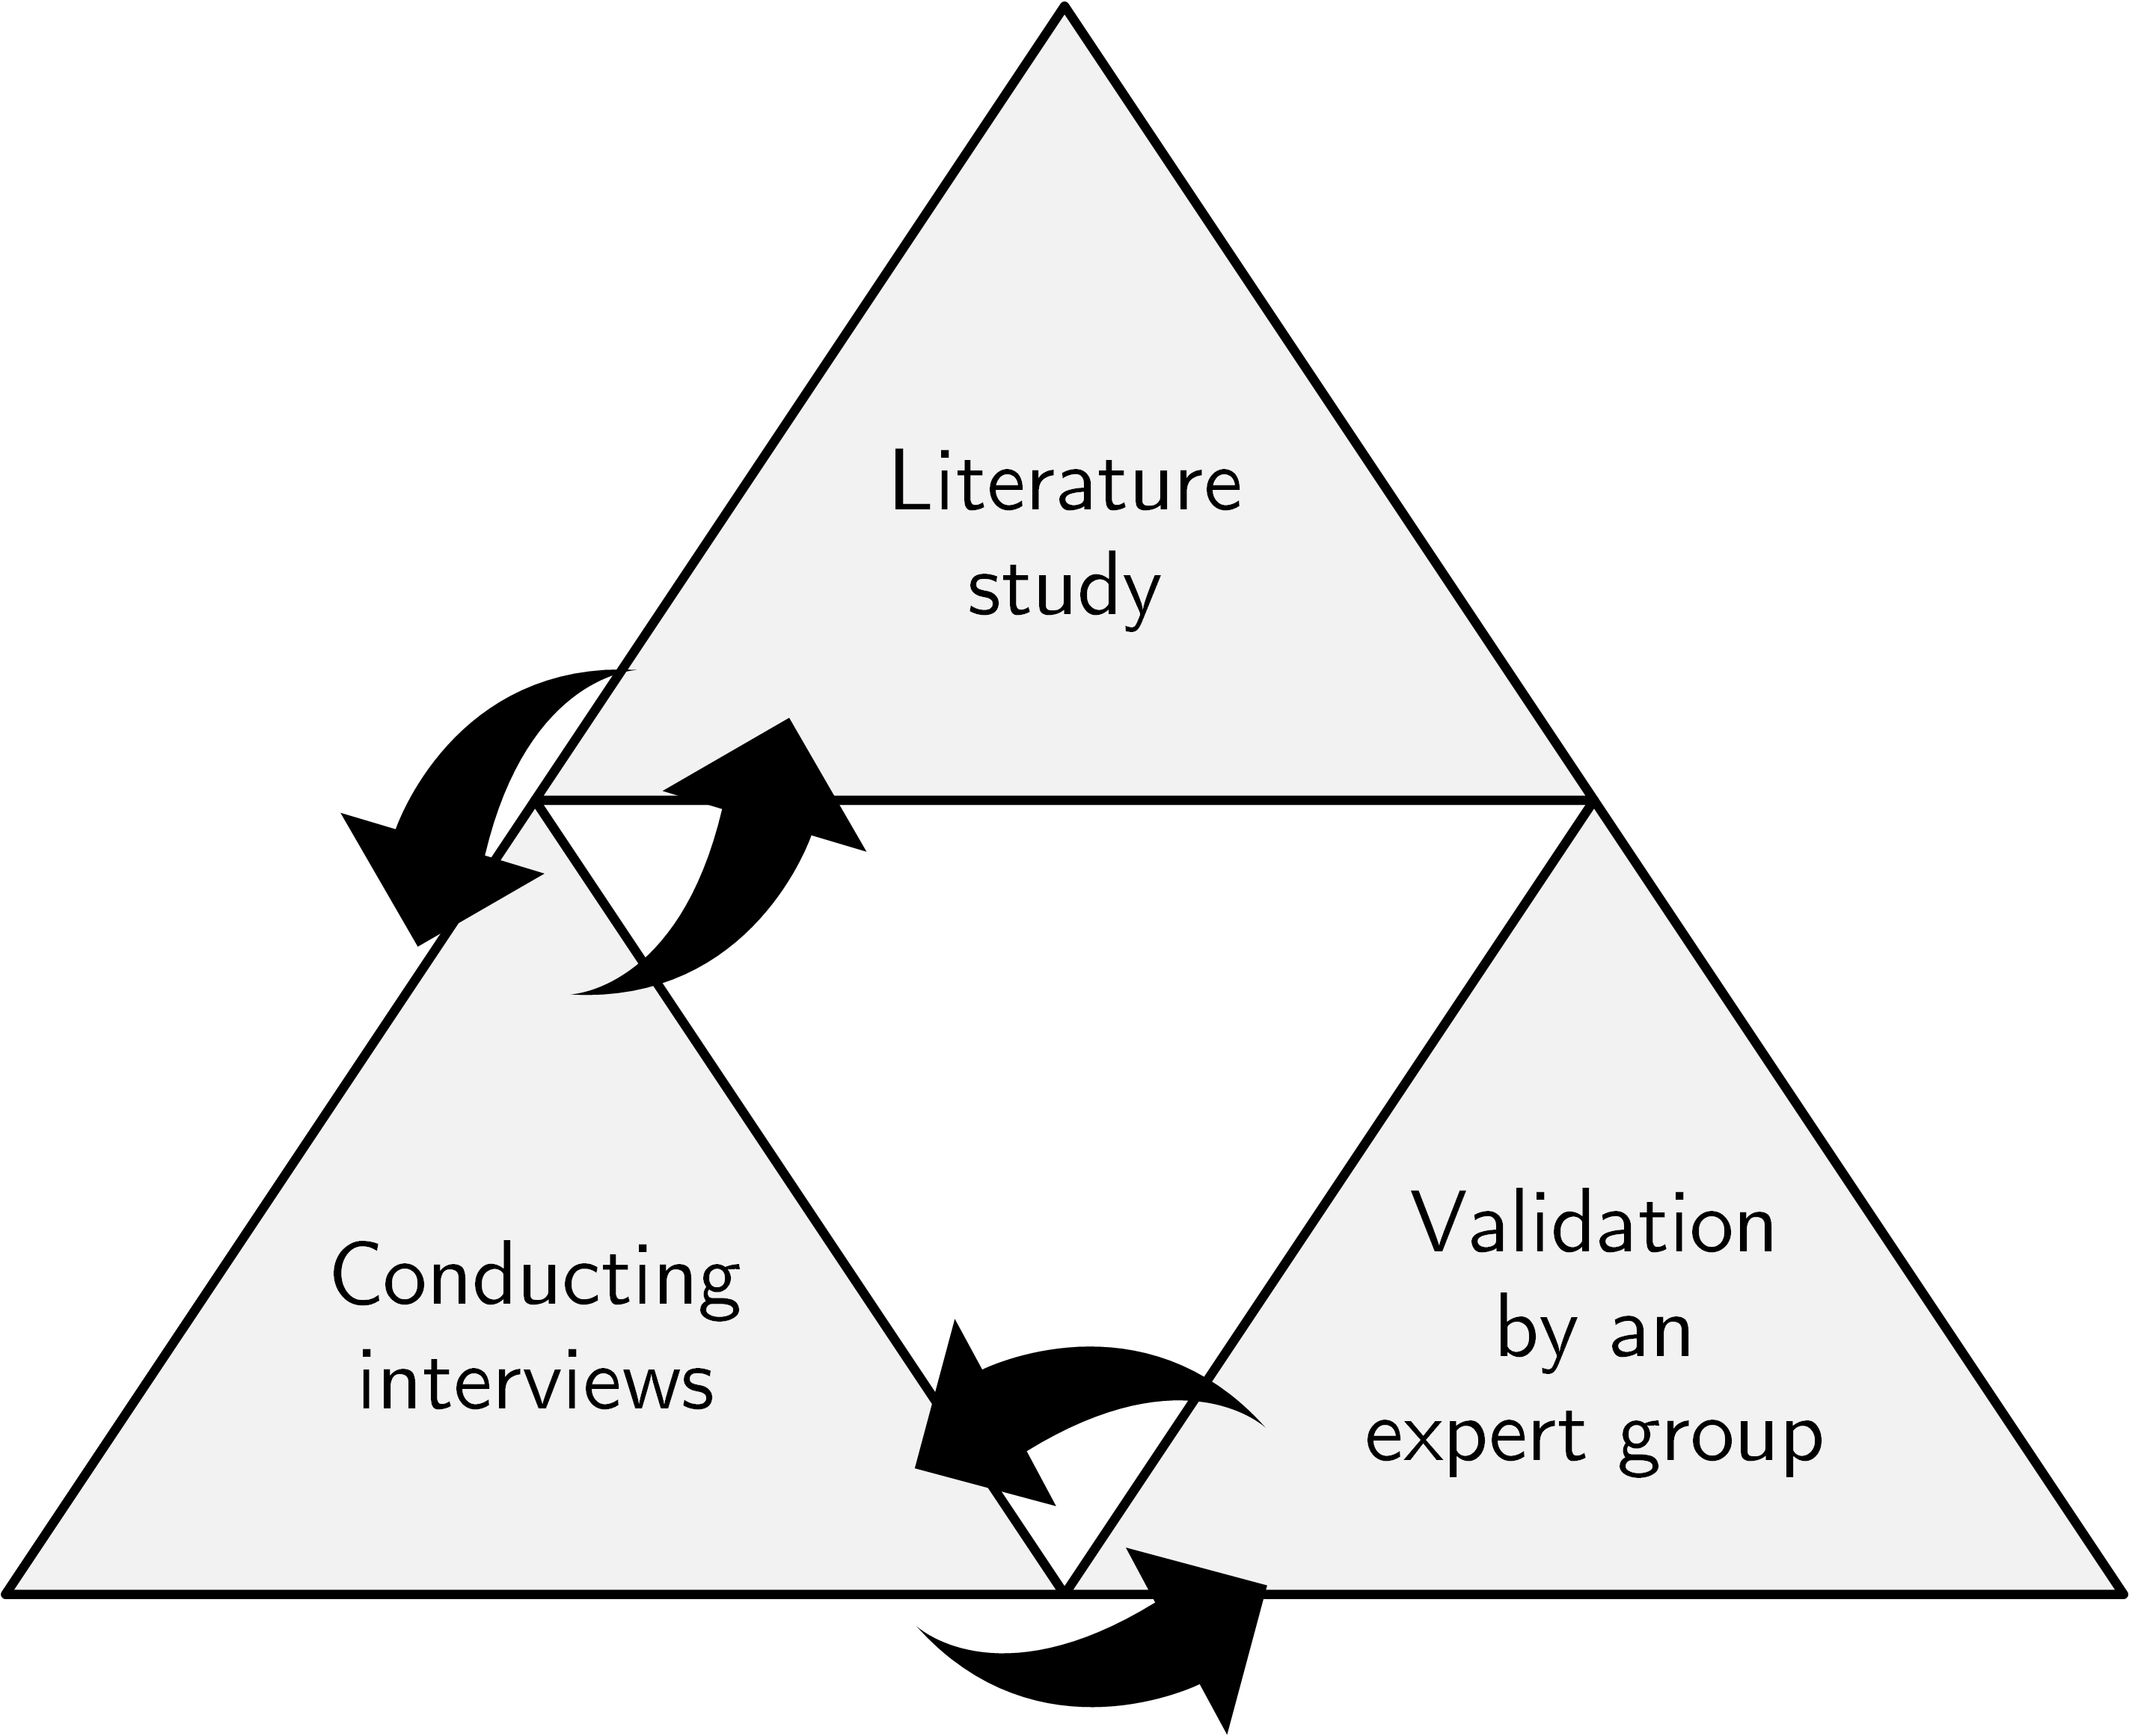
\includegraphics[width=14cm]{images/researchmodel.png}
		\caption[Research Model]{Research Model}
		\label{fig:research-model}
	\end{figure}

In the first phase of research (a), I conduct preliminary research and I study different theories and definitions of the involved concepts. The output of the first phase is the definitions and theories relevant to this research, such as \gls{antifragile}, \acrlong{ea}, the public Ssctor market, and \acrshort{vuca}. In the second phase of research (b), I confront \gls{antifragile} with \acrlong{ea} and the public sector market with \acrshort{vuca}. I am using interviews to validate the confrontation between the public sector Market with \acrshort{vuca}. The outcome of the second phase is the initiation of analysis on success factors of \acrlong{ea} relevant for contribution to \gls{antifragile} and analysis on attributes of the public sector market influenced by \acrshort{vuca} (c). In the fourth phase (d), I used the output of the analysis to confront the success factors with a Delphi Group for validation through the Delphi Method to conclude and discuss his research (e).

\begin{remark}
	Missing the outcome of the confrontation of (a) that is used by all concepts in (b).
\end{remark}
\section{Research quality}
\label{sec:researchquality}
I use three frameworks to guide me to increase the rigorousness of the research.
\begin{itemize}
	\item{Quality Principles of \textcite{Recker2013} (subsection \ref{sub:recker}).}
	\item{The FAIR Principles from Scientific Data (subsection \ref{sub:fair}).}
	\item{The Open Science Framework (subsection \ref{sub:osf}).}
\end{itemize}
\subsection{Quality Principles of Recker}
\label{sub:recker}
The first framework is that of \textcite[p. 16-17]{Recker2013} who uses four important principles:
\begin{itemize}
	\item{\textbf{Replicability} is a term that characterises the extent to which research procedures are repeatable. The principle states that the procedures by which research outputs are created should be conducted and documented in a manner that allows others outside the research team to independently repeat the procedures and obtain similar, if not identical, results.}
	\item{\textbf{Independence} is closely related to reliability. It concerns the extent to which the research conduct is impartial and freed from any subjective judgment or other bias stemming from the researcher or research team itself.}
	\item{\textbf{Precision} states that in all scientific research the concepts, constructs, and measurements should be as carefully and precisely defined as possible to allow others to use, apply, and challenge the definitions, concepts, and results in their own work.}
	\item{\textbf{Falsification} describes the logical possibility than an assertion, hypothesis, or theory can be contradicted by an observation or other outcome of a scientific study or experiment.}
\end{itemize}
\begin{remark}
	Howto falsify? 
\end{remark}
\subsection{Fair Principles}
\label{sub:fair}
In 2016, the 'FAIR Guiding Principles for scientific data management and stewardship' were published in Scientific Data. The authors intended to provide guidelines to improve the Findability, Accessibility, Interoperability, and Reuse of digital assets. The research is using the FAIR Principles\footnote{\url{https://www.go-fair.org/fair-principles/}} to increase the quality of the published thesis.
\begin{itemize}
	\item{\textbf{Findable.} The first step in (re)using data is to find them. Metadata and data should be easy to find for both humans and computers. Machine-readable metadata are essential for automatic discovery of datasets and services. The thesis, research and used datasets are containing keywords, links, and structures that can be indexed.}
	\item{\textbf{Accesible.} Once the user finds the required data, she/he/they need to know how can they be accessed. The thesis, research and used datasets are published on GitHub, Zenodo, and Researchgate based on Open Access. I create objects containing a location on where the data can be acquired if it cannot be published because of author rights.}
	\item{\textbf{Interoperable.} The data usually need to be integrated with other data. In addition, the data need to interoperate with applications or workflows for analysis, storage, and processing. This principle is not relevant for this research. The data are qualitative data sets based on literature, interviews, and questionnaires.}
	\item{\textbf{Reusable.} The ultimate goal of FAIR is to optimise the reuse of data. To achieve this, metadata and data should be well-described so that they can be replicated and/or combined in different settings. The thesis, research and used datasets are published under the \href{https://creativecommons.org/licenses/by-sa/4.0/}{\ccbysa\ CC-BY-SA 4.0 license.} It is allowed that the thesis, research, and datasets are shared and are adapted (even commercially) as long as the original author is attributed and the possible derivate is published under the same license.}
\end{itemize}
\subsection{The Open Science Framework}
\label{sub:osf}
One of the starting points of the research is Open Science. The idea behind Open Science is to allow scientific information, data and outputs to be more widely accessible (Open Access) and more reliably harnessed (Open Data) with the active engagement of all the stakeholders (Open to Society) \parencite{UNESCO2020}. The Center for Open Science\footnote{{\url{https://www.cos.io/}}} supports this way of research by supplying guidelines and even a toolkit. For this research the toolkit is used to support Open Access, Open Data and Open to Society. One of the tools in the toolkit is a reference model to select tools for the four main phases of research: Search and Discover, Design Study, Collect and Analyse Data, and Publish Reports. I use this reference model in section \ref{sec:researchinfraandtooling}. Using this framework will help in achieving replicability, precision, and reusability.
\section{Research approach}
\label{sec:researchapproach}
In this section, I describe the approach of the research. This description helps to increase replicability, independence, and reusability. For this research approach, I follow the research model (figure \ref{fig:research-model}) and the research (sub)questions (section \ref{sec:researchsubject}). The research model contains five phases in the research. The five phases are used to describe the research approach. The five phases are (a) Desk research, (b) Confrontation, (c) Analysis, (d) Validation, and (e) Conclusion and discussions.

\subsection{Desk research}
\label{sub:deskresearchphase}
The first phase of the research model emphasises desk research on the relevant concepts, theories and definitions. Desk research is conducted based on a literature study. The main concepts of \gls{antifragile}, \acrshort{ea}, \acrshort{vuca}, and the public sector are studied. This first phase (a) will answer the sub-questions of:
\begin{itemize}
	\item{What is literature saying about \gls{antifragile}?}
	\item{What is literature saying about the public sector?}
	\item{What is literature saying about \acrlong{ea}?}
	\item{What is literature saying about the success factors of Enterprise Architecture?}
\end{itemize}

\subsubsection{Literature research}
For the literature research two primary methods are used. The first method is (foward and backward) snowballing of already acquired literature. The second method is the use of online scientific libraries.

\begin{figure}[H]
	\centering
	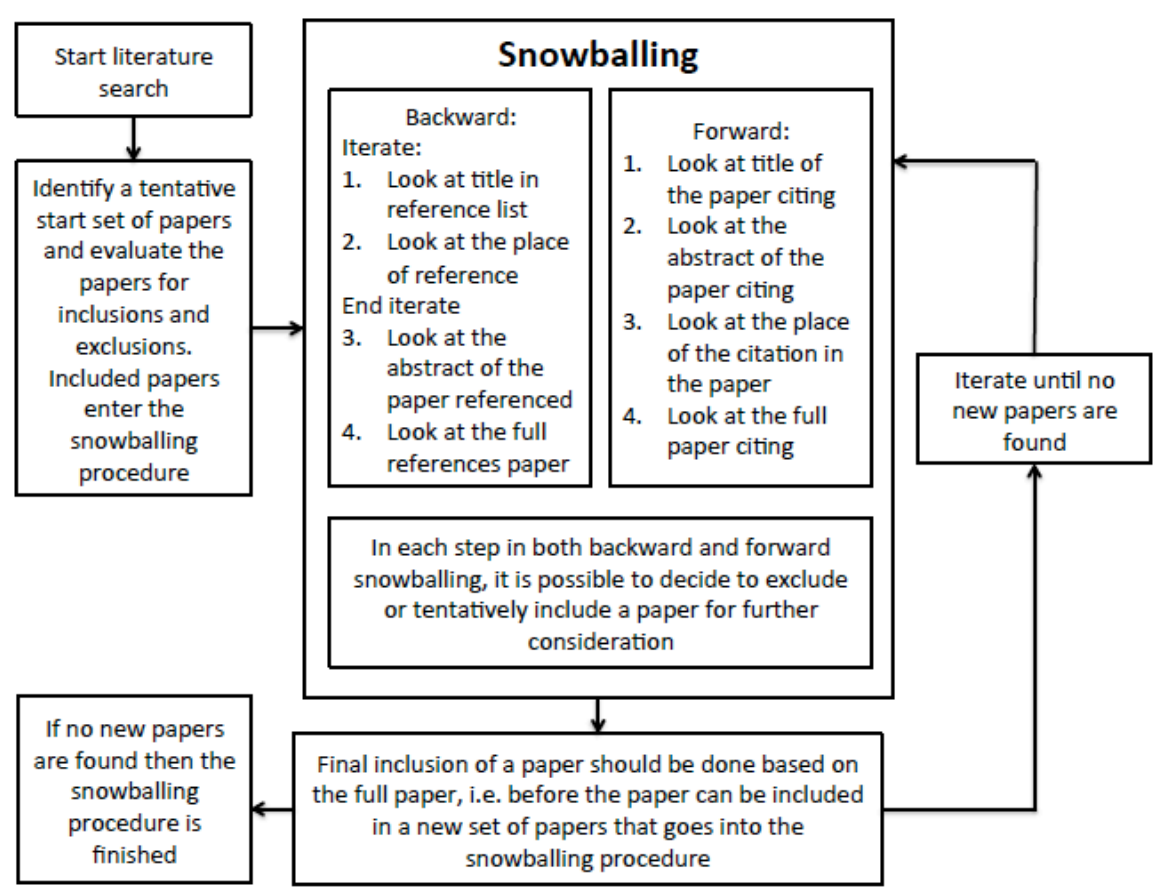
\includegraphics[width=0.6\linewidth]{images/snowball}
	\caption[Snowballing literature]{Snowballing literature \parencite{Botjes2021a}}
	\label{fig:snowball}
\end{figure}

For finding relevant literature online scientific libraries are used. The online scientific libraries are Web of Science, Research Gate, and Google Scholar. The full concept name is used and the known abbreviations of the concept (e.g. Enterprise Architecture and EA). The list of abbreviations contains the used abbreviations. Literature is only accepted if the literature complies with quality attributes. These attributes are accuracy, authority, objectivity, currency, and coverage\footnote{\url{https://libguides.library.cityu.edu.hk/litreview/evaluating-sources/}}. All found literature is administrated for replicability, independence, precision, accessibility, and reusability. Section \ref{sub:tbresearchexecution} describes how literature registration and administration is executed.

\subsubsection{Antifragile}
\label{subsub:antifragile}
The literature study on \gls{antifragile} makes use of four primary sources. The first primary source is the book ''\Gls{antifragile}: Things that gain from disorder'' \parencite{Taleb2012}. \textcite{Taleb2012} is the progenitor of the \gls{antifragile} theory. The second primary source is the master thesis ''Defining \Gls{antifragility} and the application on Organisation Design" \parencite{Botjes2020}. \citeauthor{Botjes2020} studied the literature, extensively, in the field of \gls{antifragile} and the application in the context of an organisation. By using the thesis of \citeauthor{Botjes2020} the literature study of this study concentrates on the literature after 2018. The last two primary resources are the articles ''No More Snake Oil: Architecting \Gls{agility} through \Gls{antifragility}'' and ''The Philosophy of Residuality Theory'' \parencite{OReilly2019,OReilly2021}. \textcite{Botjes2020} did not use the articles of \citeauthor{OReilly2019}. The theories of \citeauthor{OReilly2019} were less of interest for the subject of \citeauthor{Botjes2020}. While for this research the Residuality Theory of \textcite{OReilly2021} has added value since it targets system architecture.

\begin{remark}
	Need to add second book from Taleb (Black Swan) since Antifragile is an answer to black swan events.\\
	Need to add book of Hole as it is one of the sources referenced by many.
\end{remark}

The first method for literature study is snowballing. Snowballing of these sources is used to determine other important literature on \gls{antifragile}. Forward snowballing is used for the source of \citeauthor{Taleb2012}. Since \citeauthor{Taleb2012} is the progenitor, it is not necessary to do a backward snowballing. Backward snowballing is used for the sources from \citeauthor{Botjes2020} and \citeauthor{OReilly2019}.

The second method for literature study is the use of online scientific libraries. For these libraries the following set of keywords or key sentences are used.
\bigskip

\begin{table}[H]
	\centering
\begin{tabular}{p{0.4\textwidth}p{0.4\textwidth}}
	\toprule
	\gls{antifragile}	& \gls{antifragile} \gls{robust} \gls{resilient} \gls{agile}\\%
	\gls{antifragile} \acrlong{ea}	& \gls{antifragile} public sector\\%
	\gls{antifragile} success factors & residuality theory\\%
	\gls{antifragile} residuality theory & \acrlong{vuca} \\%
	\gls{antifragile} system & \\%
	\bottomrule
\end{tabular}
	\caption{Antifragile keywords}
\end{table}

\subsubsection{Enterprise Architecture}
\label{subsub:enterprisearchitecture}
The literature study on \acrshort{ea} makes use of three primary sources. \textcite{Greefhorst2011} is a book on the theory on steering mechanisms of \acrshort{ea} with the emphasis on the use of principles. \textcite{Ross2014} is the most referenced book on the subject \acrshort{ea} and Business Strategy. The last one is the article of \textcite{Lapalme2012} who researched the different manifestations of \acrshort{ea}.

The first method is snowballing. All three sources will be used for forward and backward snowballing. The second method for literature study is the use of online scientific libraries. For these libraries the following set of keywords and key sentences are used:
\bigskip

\begin{table}[H]
	\centering
\begin{tabular}{p{0.4\textwidth}p{0.4\textwidth}}
	\toprule
	\acrlong{ea} & \acrlong{ea} sucess factors\\%
	\acrlong{ea} \gls{antifragile} system	& \acrlong{ea} steering mechanism\\%
	intentional emergent \acrlong{ea} & \acrlong{ea} Business Strategy\\%
	\acrlong{ea} public sector & \\%
	\bottomrule
\end{tabular}
	\caption{Enterprise Architecture keywords}
\end{table}

\subsubsection{Public sector}
\label{subsub:publicsector}
The literature study on public sector makes use of one primary source. \textcite{Wal2008} is an article on the differences between the public and private sector based on the core values of these sectors. This article is used for forward and backward snowballing. The last method for literature study is the use of online scientific libraries. For these libraries the following set of keywords and key sentences are used:
\bigskip

\begin{table}[H]
	\centering
	\begin{tabular}{p{0.4\textwidth}p{0.4\textwidth}}
		\toprule
		Difference public and private sector &	public sector \gls{antifragile}\\%
		Collaboration public and private sector & public sector \gls{resilient}\\%
		public sector \acrshort{vuca} & \\%
		\bottomrule
	\end{tabular}
	\caption{Public sector keywords}
\end{table}

\begin{remark}
	The preliminary research on the topic public sector is not started yet. Maybe some primary sources will emerge.
\end{remark}

\subsection{Confrontation}
\label{sub:confrontationphase}

For the confrontation of VUCA with the public sector interviews are used to....\\
For the confrontation of EA with EA a framework/model is needed! (part of Theoretical background)

\begin{remark}
	What is the model for confrontation?
	I have to determine the lens I am going to use.
\end{remark}

The second phase (b) 

\subsection{Analysis}
\label{sub:analysisphase}

\begin{remark}
	What is the model for Analysis?
	I have to determine the lens I am going to use.
\end{remark}

The third phase (c)

How can the success factors of \acrlong{ea} contribute to becoming antifragile?

\subsection{Validation}
\label{sub:validatinphase}
%The fourth phase (d) analyses the outcome of the analysis phase. This outcome is the answer to the sub-question ''How can the success factors of \acrlong{ea} contribute to becoming antifragile?'' 
The success factors are validated by the means of the Delphi Method.

\subsubsection{Delphi Method}
\label{subsub:delphimethod}
The Delphi method is an iterative process to collect and distil the anonymous judgments of experts using a series of data collection and analysis techniques interspersed with feedback. The Delphi method is well suited as a research instrument when incomplete knowledge about a problem or phenomenon. The Delphi method evolved into a flexible research method appropriate for many \acrfull{is} research projects, such as determining the criteria for \acrshort{is} prototyping decisions, ranking technology management issues in new product development projects, and developing a descriptive framework of knowledge manipulation
activities. The Delphi method is a flexible, effective and efficient research method that can be successfully used by \acrshort{is} graduate students to answer research questions in \acrshort{is} and to advance the \acrshort{is} Body of Knowledge rigorously. \parencite{Skulmoski2007}

The group participants are mutually unknown, I am the only one who knows who the participants are. When it cannot be proven that the artefact is incorrect, it must be correct. This method is the principle of falsification. To reach a consensus, I use questionnaires. To reach a consensus, I am working iterative and adjusts the artefact after the feedback. I expect consensus on the artefact after two to six rounds of questionnaires. The goal of the Delphi Rounds is that it cannot be proven that the sucess factors are incorrect. This method is the principle of falsification (subsection \ref{sub:recker}). However, when is there a consensus? \textcite[p. 404]{Diamond2014} concludes in his research for over more than 100 cases that the median of the percentage of consensus 75\% is. I state, as a result of the research of \textcite{Diamond2014}, that consensus is reached with the threshold of 75\%. I state with some degree of certainty that the artefact is correct with a consensus of 75\%.

I defined domains for the group composition based on the context of the research. These domains are \acrfull{isv}, Municipality, National Government, VNG-Realisatie (the association of Dutch municipalities), and Academics. Participants are members of one or more of these domains and have an affinity with Enterprise Architecture and the public sector. I invite at least three participants per domain (n=3). The result is a total population of at least fifteen (n=15). The approach followed \textcite{Denzin2017} multiple triangulation approach, which encourages several methods to collect data and multiple investigators with varied expertise.

For the Delphi Group composition domains are defined based on the context of the research. These domains are \acrfull{isv}, Municipality, National Government, VNG-Realisatie (the association of Dutch municipalities), and Academics. The participants have affinity with \acrshort{ea}. The participants validate the artefact their context and domain.

Meeting Wizard is the service for sending out the questionnaires and execute the analysis of the outcome of the questionnaires. The participants get an invite by email to fill in the questionnaires. I analyse the results after every round and communicates the outcome as soon as a consensus is reached.

\subsection{Conclusion and discussion phase}
\label{sub:conclusionanddiscussinophase}
The fifth phase (e)

What are the success factors of \acrlong{ea} for \gls{antifragility} in the public Sector?

\section{Research type}

\begin{remark}
	Qualitative vs Quantitative! (use \parencite{Recker2013})
\end{remark}


\section{Research infrastructure and tooling}
\label{sec:researchinfraandtooling}
\begin{wrapfigure}{R}{0.5\textwidth}
	\begin{center}
		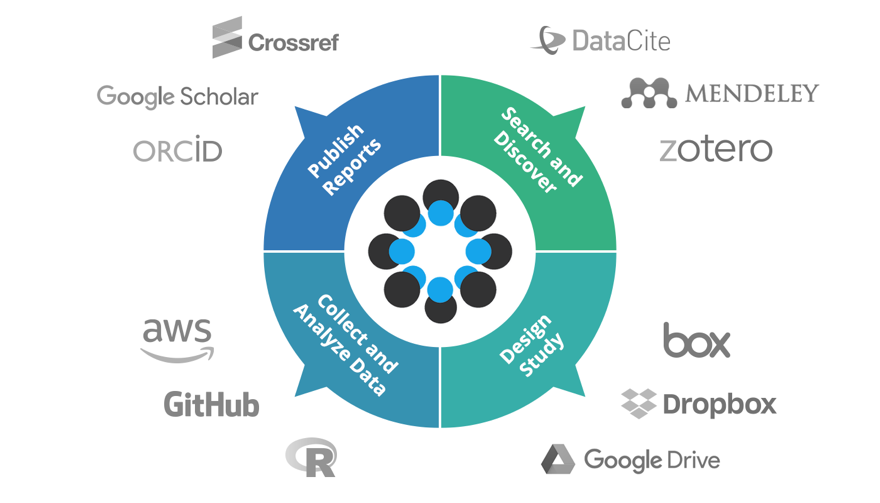
\includegraphics[width=0.5\linewidth]{images/osfframework}
		\caption[Open Science Framework]{Open Science Framework}
		\label{fig:osfframework}
	\end{center}
\end{wrapfigure}
For selecting the suitable instruments for the research, the Open Science Framework\footnote{\url{https://www.cos.io/products/osf}} is used. The Open Science Framework consists out of 4 stages in a research project. Those stages are: ''Search and Discover, Design Study, Collect and Analyse, and Publish Reports.'' The Open Science Framework proposes specific infrastructure and tools per stage. The transparency in the used infrastructure and tools increases the quality of the research. It increases the replication factor, findability, accessibility, interoperability, and reusability.
\subsection{Thesis creation}
\label{sub:tbresearchcreation}
I used my corporate laptop (Dell Latitude 7200 2-in-1\footnote{\url{https://www.dell.com/en-us/work/shop/dell-laptops-and-notebooks/latitude-7200-2-in-1-laptop/spd/latitude-12-7200-2-in-1-laptop}}) with Windows 10 Professional installed for creating the thesis. The thesis is created with the markup language \LaTeX\footnote{\url{https://www.latex-project.org/}}. The used typesetting environment is TexLive\footnote{\url{https://www.tug.org/texlive/}} with the document type of ''Report'' from KOMA-Script\footnote{\url{https://ctan.org/pkg/koma-script}}. TexStudio\footnote{\url{https://www.texstudio.org/}} is the used \LaTeX\ Editor. It supports syntax-highlighting, has an integrated viewer, reference checking and numerous wizards. For the creation and administration of references Bib\LaTeX\footnote{\url{https://ctan.org/pkg/biblatex/}} is used with the reference manager JabRef\footnote{\url{https://www.jabref.org/}} with the citation style of APA 7th Edition\footnote{\url{https://apastyle.apa.org/}} and with web browser integration. The files are stored on a personal Dropbox\footnote{\url{https://www.dropbox.com/}} that is used by GitHub Desktop\footnote{\url{https://desktop.github.com/}} to synchronise with a public GitHub repository\footnote{\url{https://github.com/JRBliekendaal/master-thesis}}. GitHub\footnote{\url{https://github.com/}} is used for source control but also for reviewing and discussing the topics with the (Co-)Promotor and the planning of the master thesis project. The thesis source files are copied to an Amazon S3 Blob\footnote{\url{https://aws.amazon.com/s3/}} for backup. The backup rotation is seven versions. Cloudberry Explorer Freeware for Amazon S3\footnote{\url{https://www.msp360.com/explorer/windows/amazon-s3.aspx}} is used for backup. Grammarly\footnote{\url{https://www.grammarly.com}}, with the paid subscription service, checks the thesis for spelling, grammar,  style, and plagiarism. The used goals for Grammarly are audience=knowledgeable, formality=formal, and domain=academic. Microsoft Visio Professional\footnote{\url{https://www.microsoft.com/en-ww/microsoft-365/visio/}} is used to create figures. The GitHub repository contains all the sources.
\subsection{Research administration}
\label{sub:tbresearchadministration}
The research administration, which includes documentation containing privacy-sensitive information, like the name and contact information of the Delphi Group participants, is stored on a non-public GitHub Repository\footnote{\url{https://github.com/JRBliekendaal/master-thesis-administration}}. The private GitHub Repository is also for staging thesis parts that still need to be anonymised. For taking notes Leuchtturm1917\footnote{\url{https://www.leuchtturm1917.us/notebook-classic.html}} Notebooks are used with mechanical pencils of Faber-Castell\footnote{\url{https://www.fabercastell.com/products/tk-fine-vario-l-mechanical-pencil-10mm-135900}} and pens from Sakura\footnote{\url{https://www.sakuraofamerica.com/product/pigma-micron/}} with long-lasting ink.
\subsection{Research execution}
\label{sub:tbresearchexecution}
For the execution of the research, Microsoft Excel\footnote{\url{https://www.microsoft.com/en-us/microsoft-365/excel}} is used for the administration of the literature research. For the administration of the literature research, the following headers are used: ID (for a unique ID per item), search terms used, scope, title, subtitle, author(s), year, type, Bib\LaTeX\ citation key, title relevance, abstract relevance, content relevance, found at, doi/isbn, url, date found, duplicate, date used, use for, and notes. Researchgate\footnote{\url{https://www.researchgate.net/}}, Web of Science\footnote{\url{https://app.webofknowledge.com/}}, and Google Scholar\footnote{\url{https://scholar.google.com/}} are the main sources for searching for literature. PaperPanda\footnote{\url{https://paperpanda.app/}} is used for hard to find literature. The literature administration is, together with the publicly available literature, stored in the repository of the master thesis. For non-public available literature, the administration contains the location where the literature is retrievable. All the literature is added to a bib\LaTeX\ file for future reference. For traceability the entries in the bib\LaTeX\ file contain the Unique ID in the notes field. JabRef is used to sort the references by using subgroups to support the workflow. The subgroups used are: ''evaluate, rejected, and used.'' Only the literature in the subgroup used are transferred to the bibliography file of the thesis. This prevents cluttering. For working as paperless as possible all the literature, where possible, is in pdf or in ebook format. For reading Acrobat Reader DC\footnote{\url{https://get.adobe.com/reader/}} is used for reading the PDF, and an Amazon Kindle Oasis\footnote{\url{https://www.amazon.com/dp/B07L5GJD99}} for eBooks. With the Amazon Kindle the highlight feature is used. This is not stored on GitHub since the highlights are under copyright of the author(s).\par
For the execution of the Delphi Method, Meetingwizard\footnote{\url{https://www.meetingwizard.nl/}} is used for questionnaires and the analysis of the questionnaires. The license for using Meeting Wizard is supplied by the Antwerp Management School.

\subsection{Summary of used infrastructure and tooling}

\begin{table}[!h]
	\begin{center}
		\begin{tabular}{@{}cccc@{}}
			\toprule
			Search \& Discover & Design Study & Collect \& Analyse Data & Publish Reports\\ \midrule
			Web of Science & 1    & JabRef   & \LaTeX \\%
			ResearchGate   &      &           & TeXstudio \\%
			Google Scholar & 2    & PaperPanda  & ORCID \\%
			Z	 & 0    & bib\LaTeX   & ResearchGate \\%
			Z	 &	x	& Meetingwizard	  & Zenodo \\%
			Z	 &	x	& Microsoft Excel  & Grammarly \\%
			Y    & 2    & GitHub  & Microsoft Visio \\%
			Y	 & 2	& Cloud Berry Explorer for S3 & \\%
			\bottomrule
		\end{tabular}
		\caption{Used infrastructure \& tooling}
		\label{tab:usedinfrastructuretooling}
	\end{center}
\end{table}

\begin{remark}
	This section needs a tabel to summarise the used tools in relation to the OSF framework.
\end{remark}				%	Add the methodology
	\chapter{Literature}

\section{Literature found after 2020}
\label{sec:literaturefoundafter2020}
Before selecting possible attributes a new search for literature was conducted with the terms as defined in \cref{sub:literaturestudy} for the concepts \gls{antifragile} and \acrshort{ea}. The search was conducted in a specific time frame. The time frame was set from 2020 to March 2022. This time frame was chosen to only search for literature that is released after the research period of \textcite{Botjes2020}. Thirty-one new articles, books and in-proceedings where found that could be of interest. For more information see Appendix~\ref{app:literaturecatchup}. Of those thirty-three new sources, three where already in the current set of literature, eight where not found or where not publicly available, thirteen where not relevant. Seven possible new sources where selected. From those seven some where not relevant or just partially.

From the seven that where left the following literature is selected for further study:

\begin{table}[H]
	\centering
	\begin{tabular}{p{.4\textwidth}p{.4\textwidth}p{0.1\textwidth}}
		\toprule%
		\textbf{Title} & \textbf{Author} & \textbf{Year} \\
		\midrule %
		blah & blah & 2020 \\%
		\bottomrule
	\end{tabular}
	\caption[Literature of interest (2020--March 2022)]{Literature of interest (2020--March 2022)}
	\label{tab:literatureafter2020}
\end{table}
				%	Add the literature chapter
	\chapter{Attributes}
\label{ch:attributes}

\section{Attributes of antifragile}
\label{sec:attributesantifragile}

\begin{figure}[h!]
	\centering
	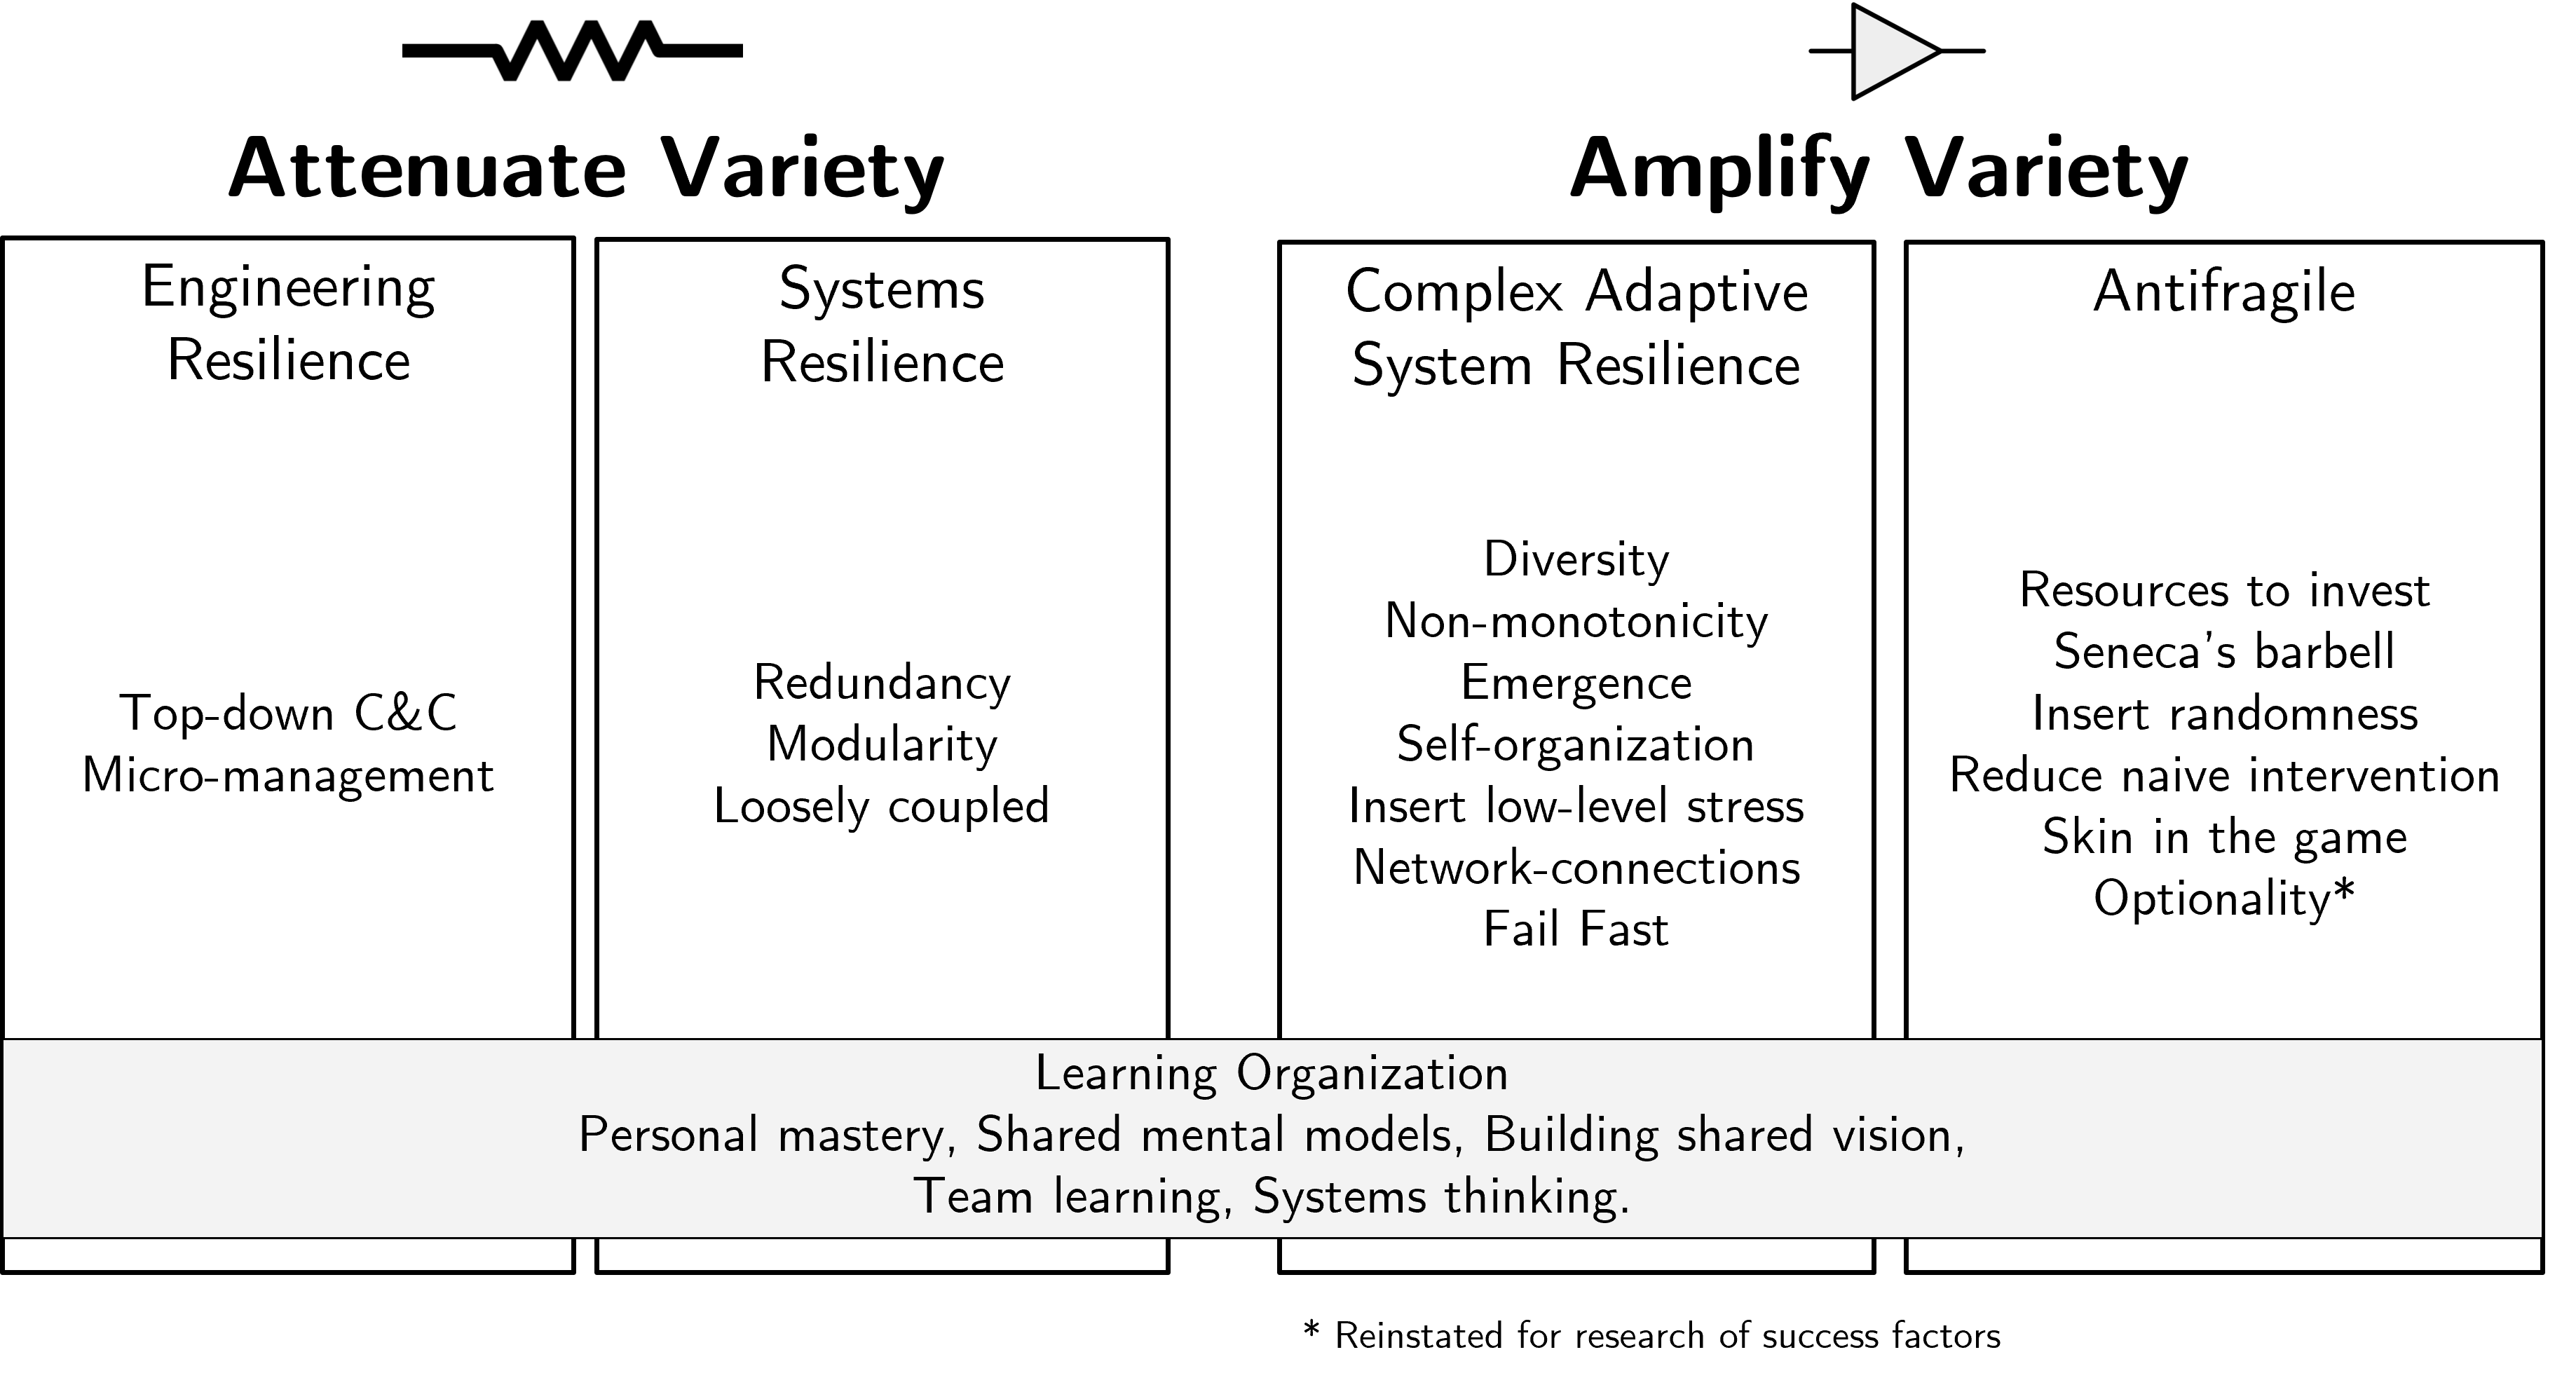
\includegraphics[width=0.8\linewidth]{images/eaalbwincludingoptionality}
	\caption[Extended Antifragile Attribute List \parencite{Botjes2021} with Optionality]{Extended Antifragile Attribute List \parencite{Botjes2021} with Optionality}
	\label{fig:eaalbwincludingoptionality-attributes}
\end{figure}

\subsection{\Gls{attenuatevariety} attributes}
\begin{table}[H]
	\begin{center}
			\begin{tabular}{@{}ll@{}}
			\toprule
				\textbf{Attribute} & \textbf{Sources} \\%
				\midrule%
				Top Down C\&C & \parencite{Botjes2020} \\%
				Micro-Management & \parencite{Botjes2020} \\%
				Redundancy & \parencite{Botjes2020} \\%
				Modularity & \parencite{Botjes2020} \\%
				Loosely coupled & \parencite{Botjes2020} \\%
			\bottomrule%
			\end{tabular}
			\caption[Attenuating attributes of \gls{antifragile}]{Attenuating attributes of \gls{antifragile}}
			\label{tab:attenuatingattributes}
\end{center}
\end{table}				

\subsection{\Gls{amplifyvariety} attributes}
\begin{table}[H]
	\begin{center}
		\begin{tabular}{@{}ll@{}}
			\toprule
			\textbf{Attribute} & \textbf{Sources} \\%
			\midrule%
			\Gls{diversity} & \parencite{Botjes2020} \\%
			\Gls{optionality} & \parencites{Taleb2012}{Gorgeon2015} \\%
			\Gls{nonmonotonicity} & \parencite{Botjes2020} \\%
			\Gls{emergence} & \parencite{Botjes2020} \\%
			\Gls{selforganisation} & \parencite{Botjes2020} \\%
			\Gls{insertlowlevelstress} & \parencite{Botjes2020} \\%
			\Gls{networkconnections} & \parencite{Botjes2020} \\%
			\Gls{failfast} & \parencite{Botjes2020} \\%
			\Gls{resourcestoinvest} & \parencites{Taleb2012}{Botjes2020} \\%
			\Gls{senecabarbell} &  \parencites{Taleb2012}{Botjes2020} \\%
			\Gls{insertrandomness} & \parencites{Taleb2012}{Botjes2020} \\%		
			\Gls{reducenaiveintervention} & \parencites{Taleb2012}{Botjes2020} \\%
			\Gls{skininthegame} & \parencites{Taleb2012}{Botjes2020} \\%
			\bottomrule%
		\end{tabular}
		\caption[Amplifying attributes of \gls{antifragile}]{Amplifying attributes of \gls{antifragile}}
		\label{tab:amplifyingattributes}
	\end{center}
\end{table}			

\subsection{\Gls{attenuatevariety} and \gls{amplifyvariety} attributes}

\begin{table}[H]
	\begin{center}
		\begin{tabular}{@{}ll@{}}
			\toprule
			\textbf{Attribute} & \textbf{Sources} \\%
			\midrule%
			\Gls{personalmastery} & \parencite{Botjes2020} \\%
			\Gls{sharedmentalmodels} & \parencite{Botjes2020} \\%
			\Gls{buildingsharedvision} & \parencite{Botjes2020} \\%
			\Gls{teamlearning} & \parencite{Botjes2020} \\%
			\Gls{systemsthinking} & \parencite{Botjes2020} \\%
			\bottomrule%
		\end{tabular}
		\caption[Attenuating and amplifying attributes of \gls{antifragile}]{Attenuating and amplifying attributes of \gls{antifragile}}
		\label{tab:attenuatingandamplifyingattributes}
	\end{center}
\end{table}	

\section{Attributes of Enterprise Architecture}
\label{sec:attributesonea}

\subsection{Enterprise IT Architecting attributes}
\label{sub:enterpriseitarchitecting}
\begin{table}[H]%
	\begin{center}%
		\begin{tabular}{@{}ll@{}}%
			\toprule%
			\textbf{Attribute} & \textbf{Sources} \\%
			\midrule%
			 & \parencite{Lapalme2012} \\%
			\bottomrule%
		\end{tabular}%
		\caption[Attributes of Enterprise Ecological Adaptation]{Attributes of Enterprise Ecological Adaptation}%
		\label{tab:attributesofenterpriseitarchitecting}%
	\end{center}%
\end{table}%


\subsection{Enterprise Integrating attributes}
\label{sub:attributesofenterpriseintegrating}
\begin{table}[H]%
	\begin{center}%
		\begin{tabular}{@{}ll@{}}%
			\toprule%
			\textbf{Attribute} & \textbf{Sources} \\%
			\midrule%
			 & \parencite{Lapalme2012} \\%
			\bottomrule%
		\end{tabular}%
		\caption[Attributes of Enterprise Integrating]{Attributes of Enterprise Integrating}%
		\label{tab:attributesofenterpriseintegrating}%
	\end{center}%
\end{table}%

\subsection{Enterprise Ecological Adaptation attributes}
\label{sub:enterpriseecologicaladaptation}

\begin{table}[H]
	\begin{center}
		\begin{tabular}{@{}ll@{}}
				\toprule
				\textbf{Attribute} & \textbf{Sources} \\%
				\midrule%
				\Gls{systeminenvironment} & \parencite{Lapalme2012} \\%
				\Gls{holisticsystemicstance} & \parencite{Lapalme2012} \\%
				\Gls{intraorganisationalcoherency} & \parencite{Lapalme2012} \\%
				\Gls{organisationallearning} & \parencite{Lapalme2012} \\%
				\Gls{environmentallearning} & \parencite{Lapalme2012} \\%
				\Gls{systeminenvironmentcoevolutionlearning} & \parencite{Lapalme2012} \\%
				\bottomrule%
			\end{tabular}
		\caption[Attributes of Enterprise Ecological Adaptation]{Attributes of Enterprise Ecological Adaptation}
		\label{tab:attributesofeea}
	\end{center}
\end{table}


				%	Add chapter on EAAF Attributes
	\chapter{Interview results}
\label{ch:interviewresults}

\section{Interviews}
\label{sec:interviews}
The interviews are in the format of semi-structured. I used a minimal set of questions. Based on the answers, the technique of hitchhiking was applied when there was a suspicion of extra information about \acrshort{ea} and \gls{antifragile} attributes. The interview summaries can be found in \cref{app:interviewsummaries}.

\begin{table}[!h]
	\label{tab:interviewquestions}
	\begin{center}
			\begin{tabular}{@{}p{0.1\textwidth}p{0.75\textwidth}p{0.15\textwidth}@{}}
				\toprule
				\textbf{Number} & \textbf{Question} & \textbf{Concept} \\ \midrule %
				1a. & How is your organisation applying \acrshort{ea}? & \acrshort{ea} \\%
				1b. & Who is accountable for \acrshort{ea} in your organisation? & \acrshort{ea} \\%
				1c. & How is \acrshort{ea} enabling your organisation to quickly adapt to changes (external influences)? & \acrshort{ea} \\%
				2a. & Does the operational model of the\gls{ps} \gls{foster} \gls{agility}? & \Gls{antifragile} \\%
				2b. & How is the \acrshort{ea} of your organisation contributing to \gls{foster} \gls{agility} in the \gls{ps}? & \acrshort{ea} \\%
				3a. & How does the public sector deal with \gls{uncertainty}? & \Gls{antifragile} \\%
				3b. & How is the \acrshort{ea} of your organisation contributing to dealing with \gls{uncertainty} in the \gls{ps}?
				 & \acrshort{ea} \\%
				4a. & How is the public sector dealing with unexpected events? & \Gls{antifragile} \\%
				4b. & How is \acrshort{ea} of your organisation contributing to dealing with unexpected events in the \gls{ps}? & \acrshort{ea} \\%
				5a. & Could you describe the risk appetite of the \gls{ps}? & \Gls{antifragile} \\%
				5b. & How does the \acrshort{ea} of your organisation match the risk appetite of the \gls{ps}?
				  & \acrshort{ea} \\%
				6a. & How is \gls{diversity} and \gls{optionality} used in the \gls{ps}? & \Gls{antifragile} \\%
				6b. & How does \acrshort{ea} of your organisation support \gls{diversity} and \gls{optionality} in the \gls{ps}? & \acrshort{ea} \\%																								
				Closing & Did you miss an important subject or do you want to add something else? & non-specific \\%
				\bottomrule
			\end{tabular}
		\caption{Interview questions}
	\end{center}
\end{table}

\section{Summary of interviews}

\section{interview results}
\subsection{Engineering Resilience}
\begin{figure}[H]
	\centering
	\begin{subfigure}[H]{0.5\textwidth}
		\centering
		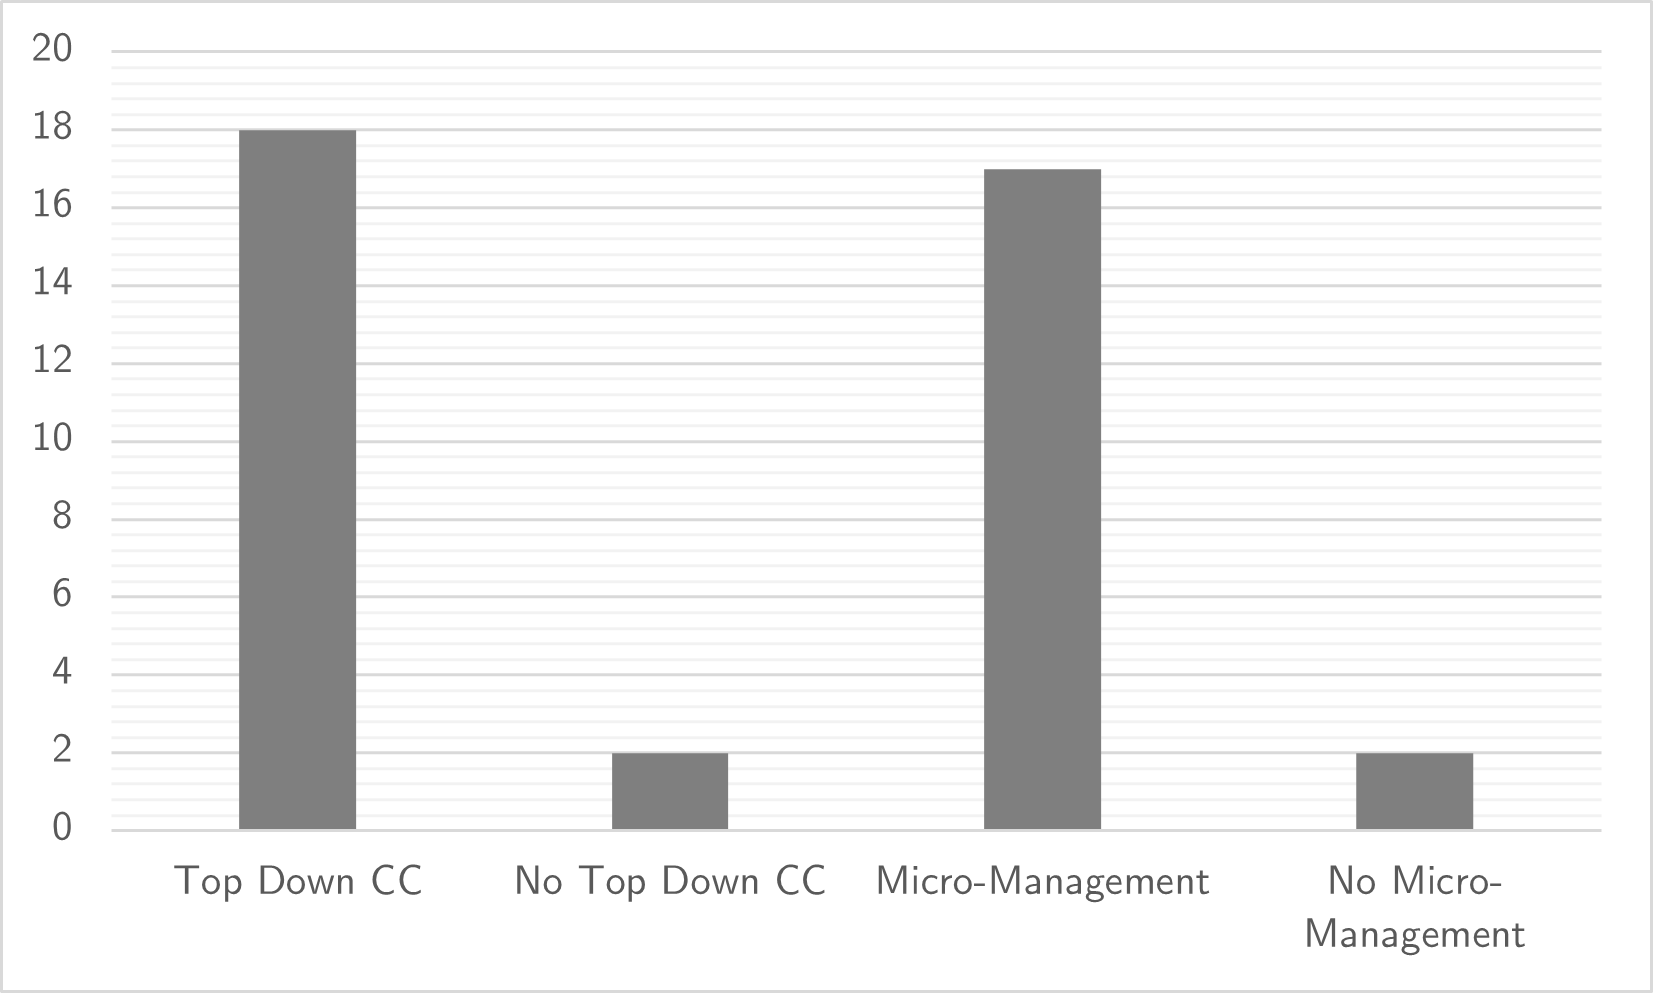
\includegraphics[width=0.95\linewidth]{images/engineeringresilience_frequency}
		\caption{Engineering Resilience Frequency}
		\label{fig:engineeringresiliencefrequency}
	\end{subfigure}%
	\begin{subfigure}[H]{0.5\textwidth}
		\centering
		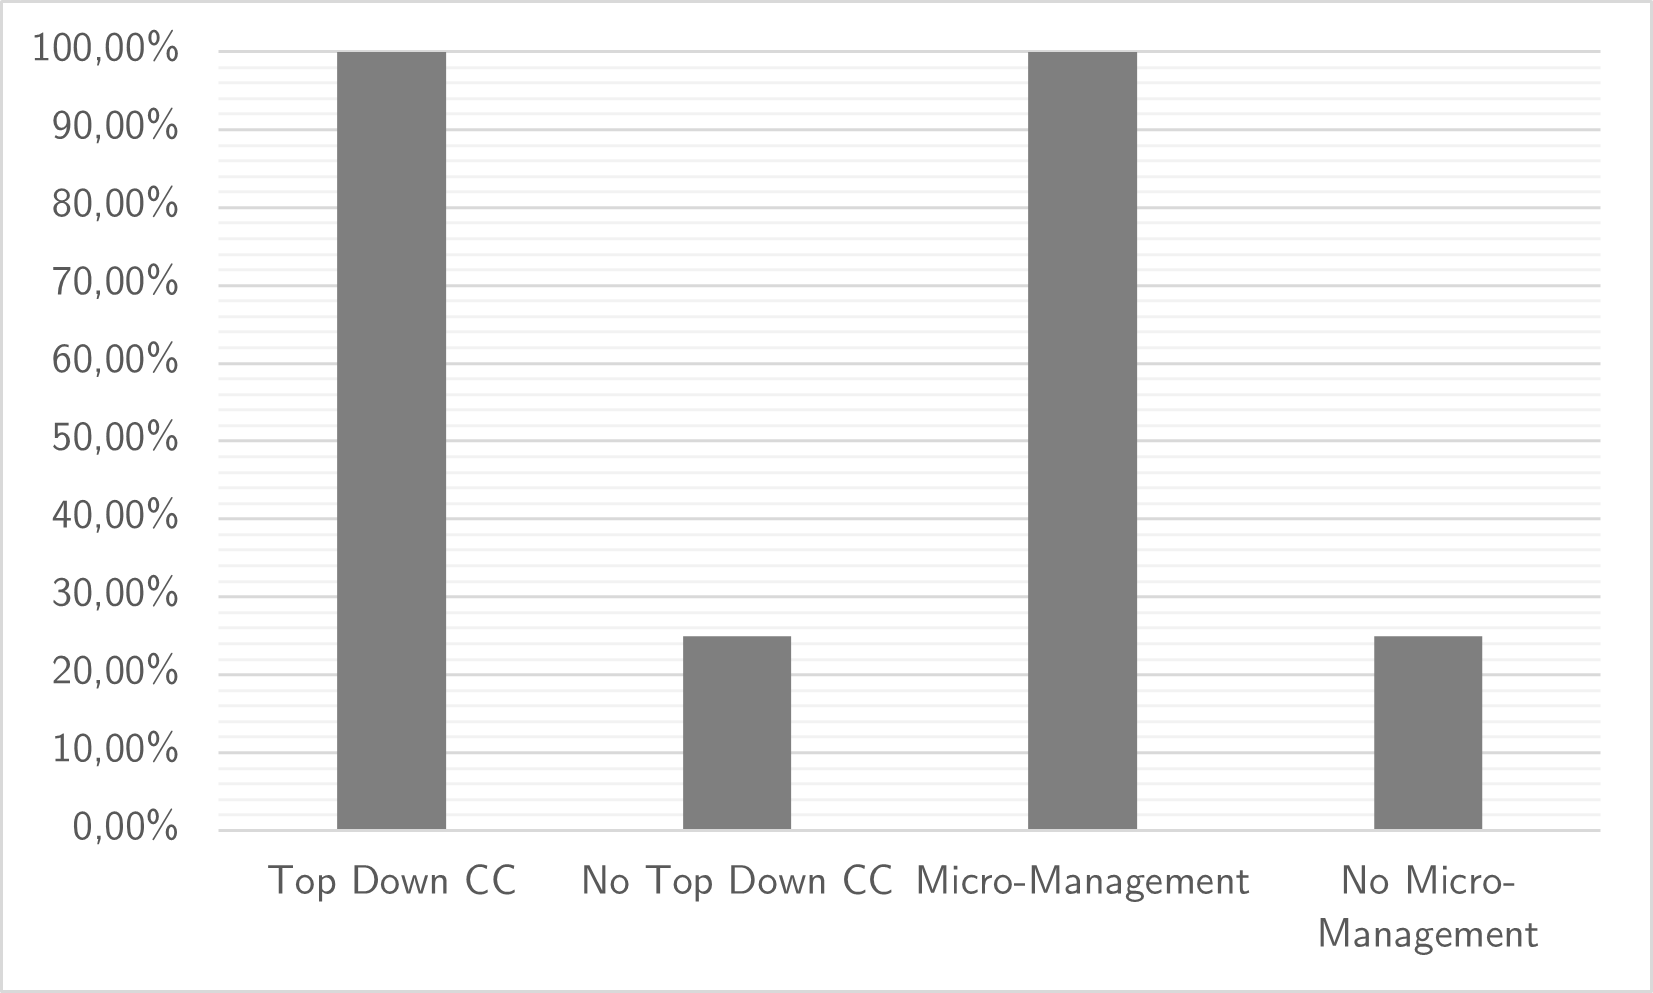
\includegraphics[width=0.95\linewidth]{images/engineeringresilience_cases}
		\caption{Engineering Resilience \% Cases}
		\label{fig:engineeringresiliencecases}
	\end{subfigure}
	\caption{Interview results Engineering Resilience}
	\label{fig:interviewresultsengineeringresilience}
\end{figure}

\subsection{Systems Resilience}
\begin{figure}[H]
	\centering
	\begin{subfigure}[H]{0.5\textwidth}
		\centering
		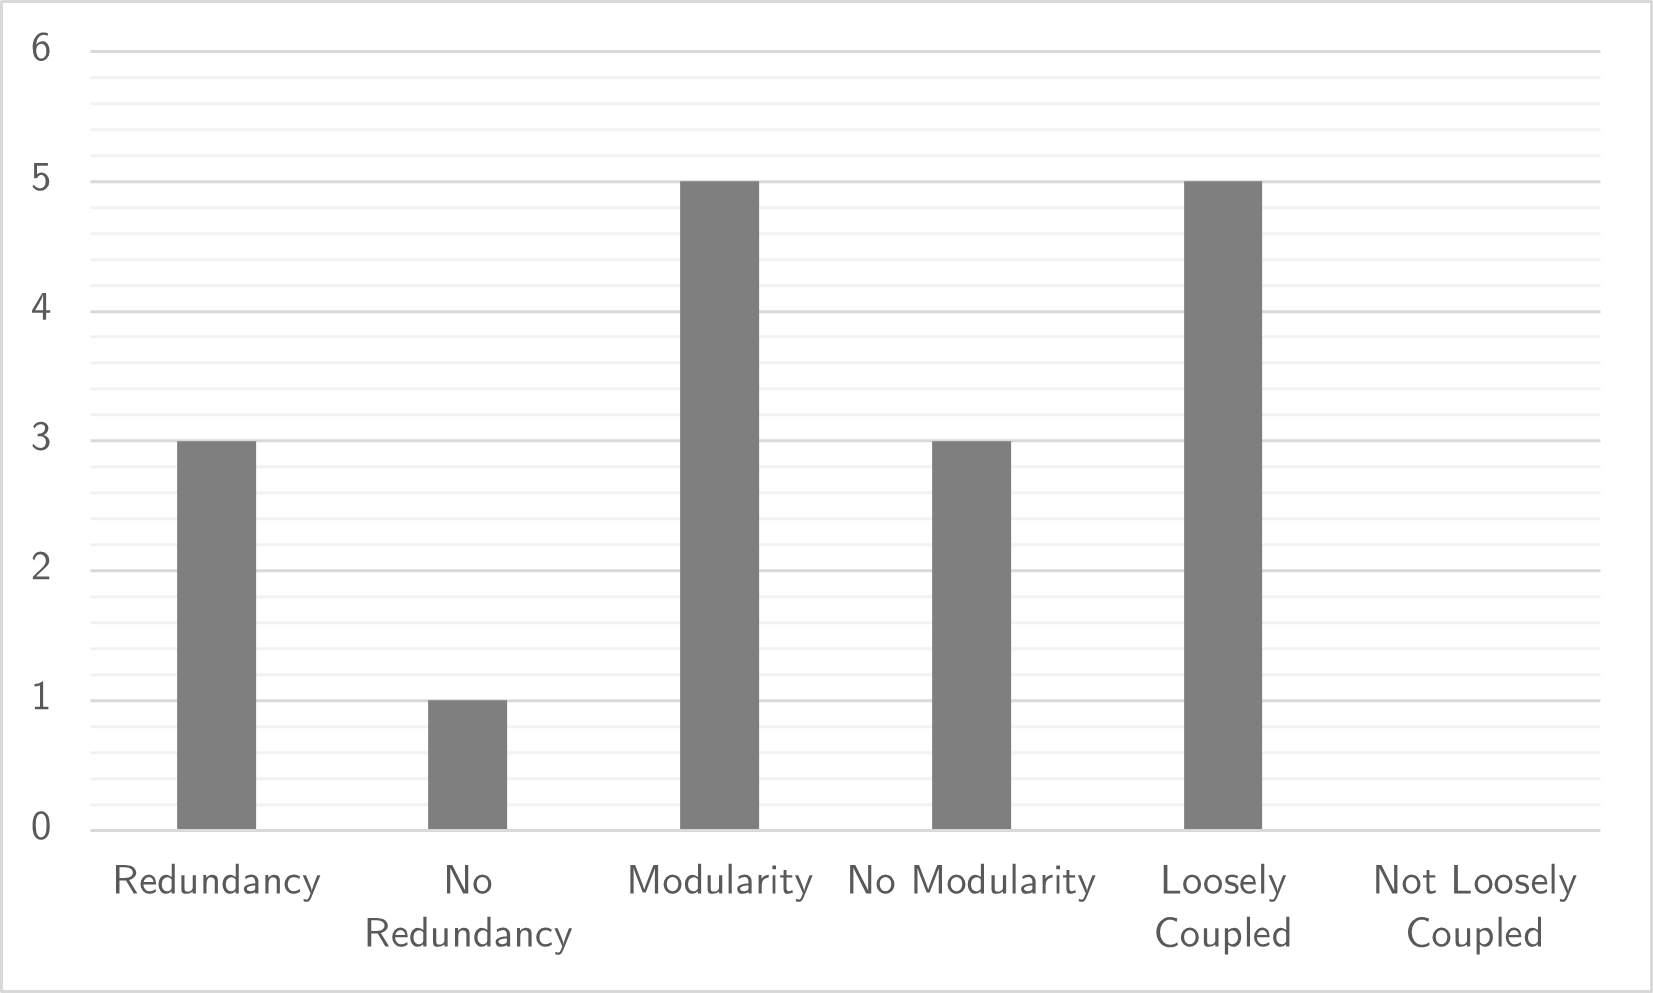
\includegraphics[width=0.95\linewidth]{images/systemsresilience_frequency}
		\caption{Systems Resilience Frequency}
		\label{fig:systemsresiliencefrequency}
	\end{subfigure}%
	\begin{subfigure}[H]{0.5\textwidth}
		\centering
		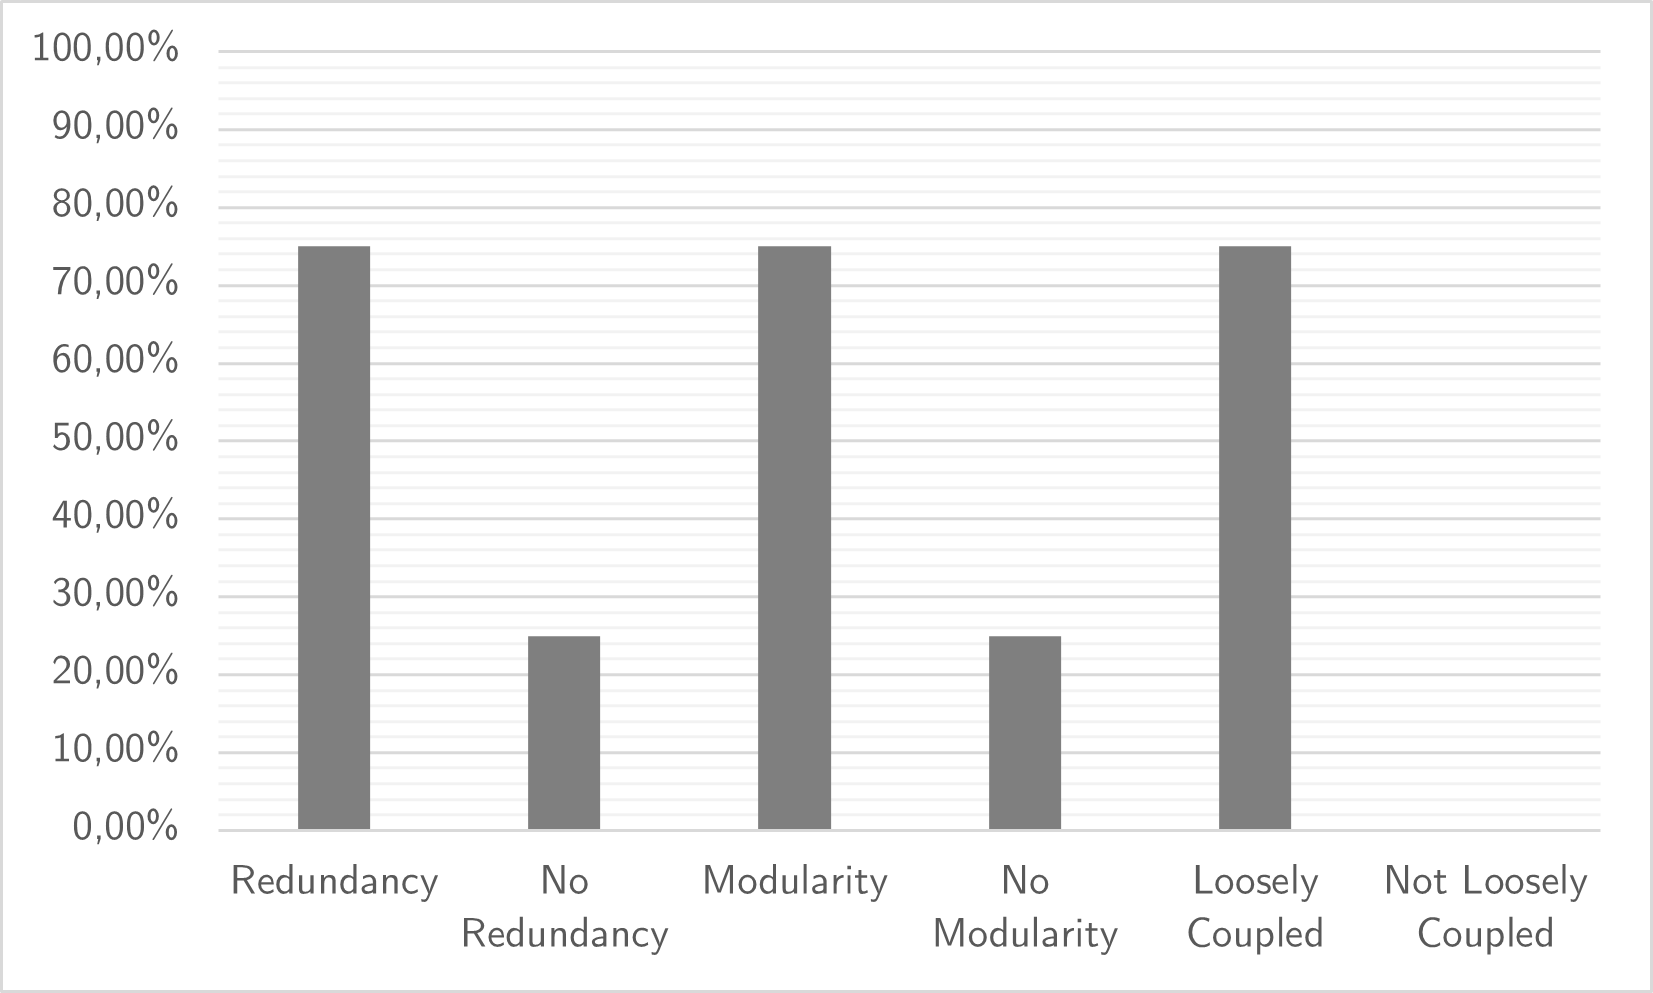
\includegraphics[width=0.95\linewidth]{images/systemsresilience_cases}
		\caption{Systems Resilience \% Cases}
		\label{fig:systemsresiliencecases}
	\end{subfigure}
	\caption{Interview results Systems Resilience}
	\label{fig:interviewresultssystemsresilience}
\end{figure}

\subsection{Complex Adaptive System Resilience}
\begin{figure}[H]
	\centering
	\begin{subfigure}[H]{0.5\textwidth}
		\centering
		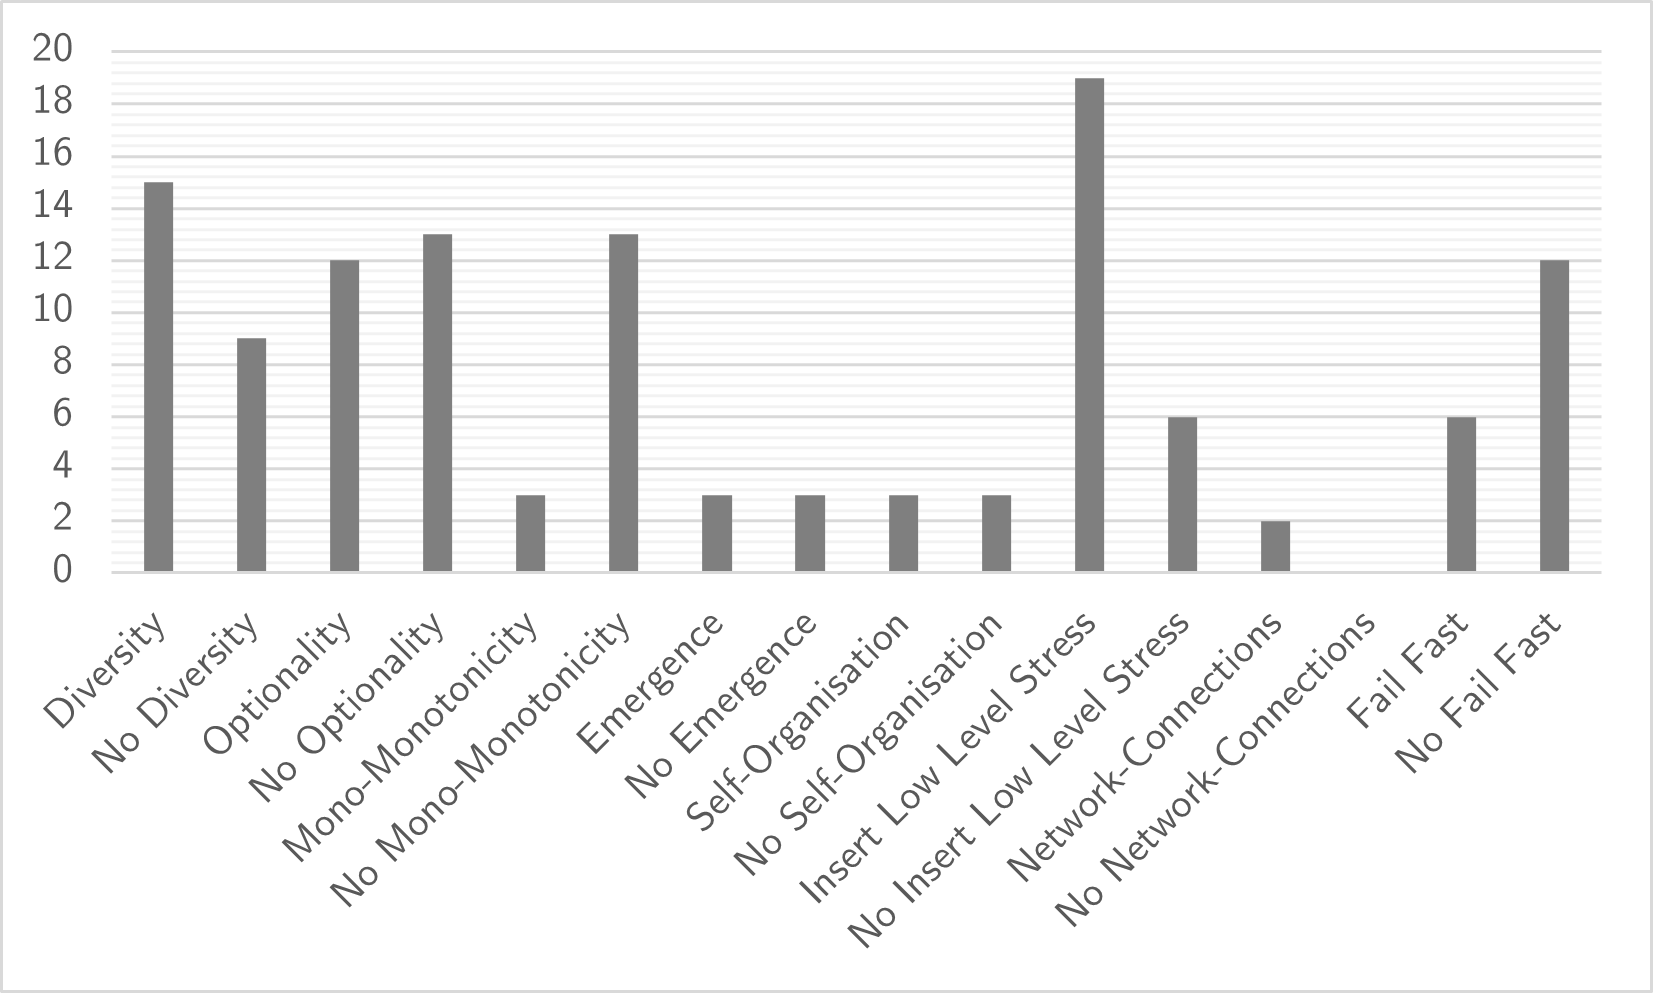
\includegraphics[width=0.95\linewidth]{images/cas_frequency}
		\caption{CAS Resilience Frequency}
		\label{fig:casfrequency}
	\end{subfigure}%
	\begin{subfigure}[H]{0.5\textwidth}
		\centering
		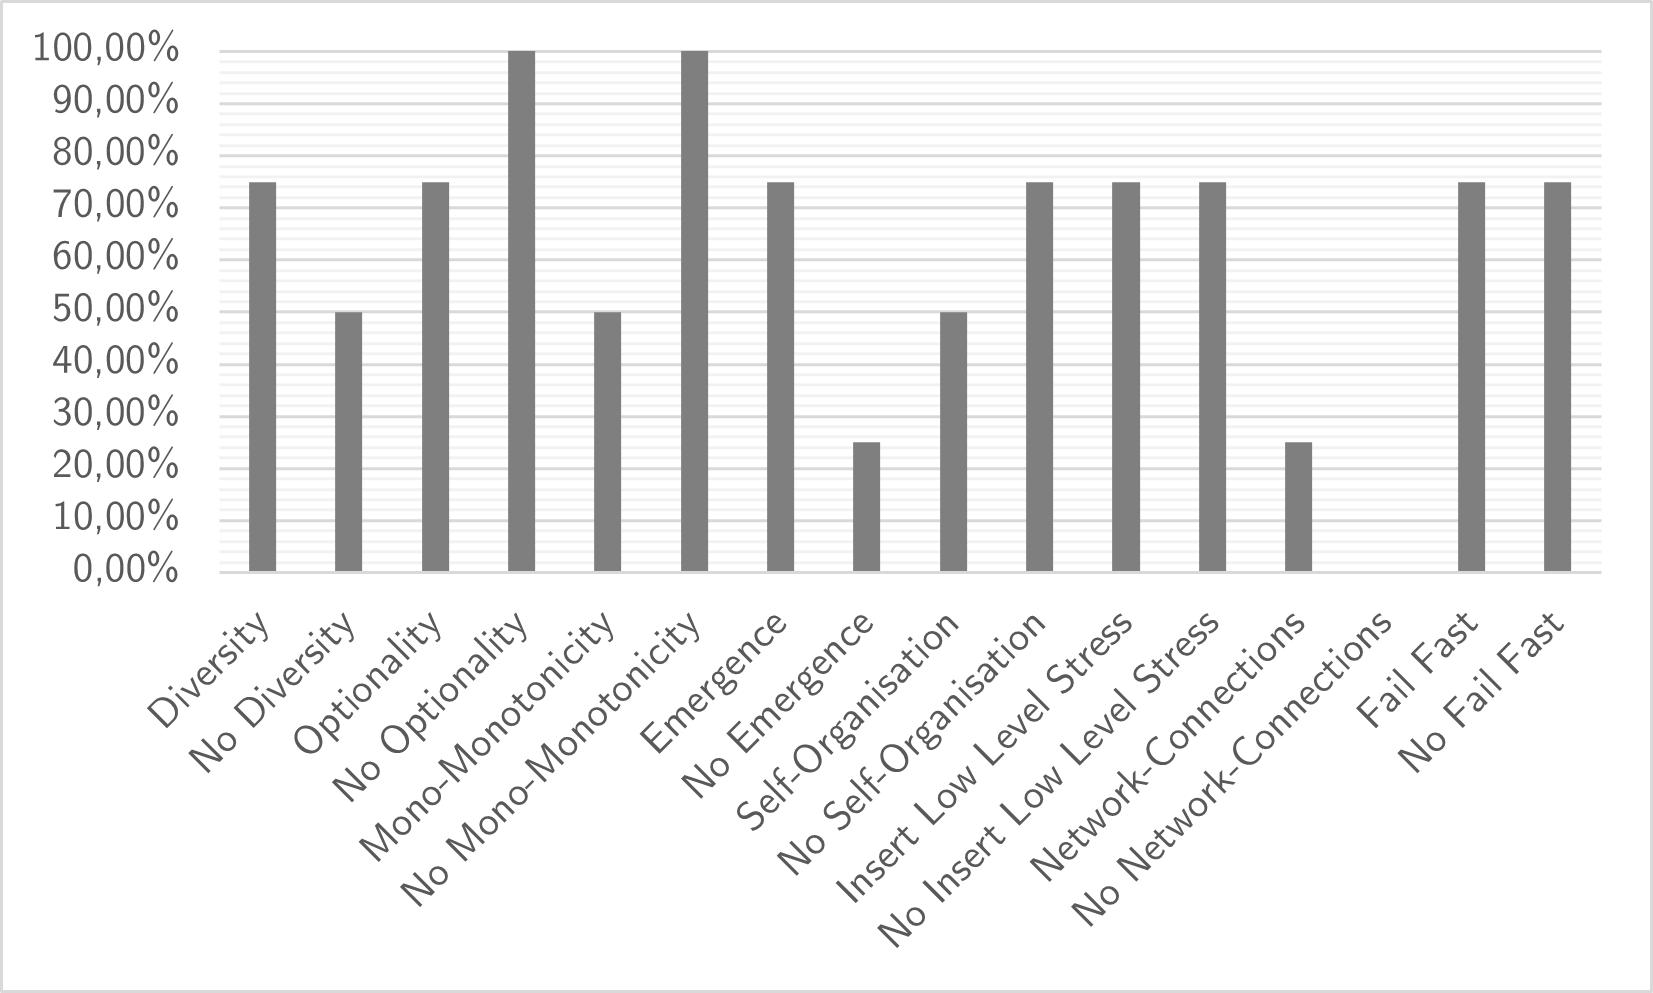
\includegraphics[width=0.95\linewidth]{images/cas_cases}
		\caption{CAS Resilience \% Cases}
		\label{fig:cascases}
	\end{subfigure}
	\caption{Interview results CAS Resilience}
	\label{fig:interviewresultscas}
\end{figure}
\subsection{Antifragile}
\begin{figure}[H]
	\centering
	\begin{subfigure}[H]{0.5\textwidth}
		\centering
		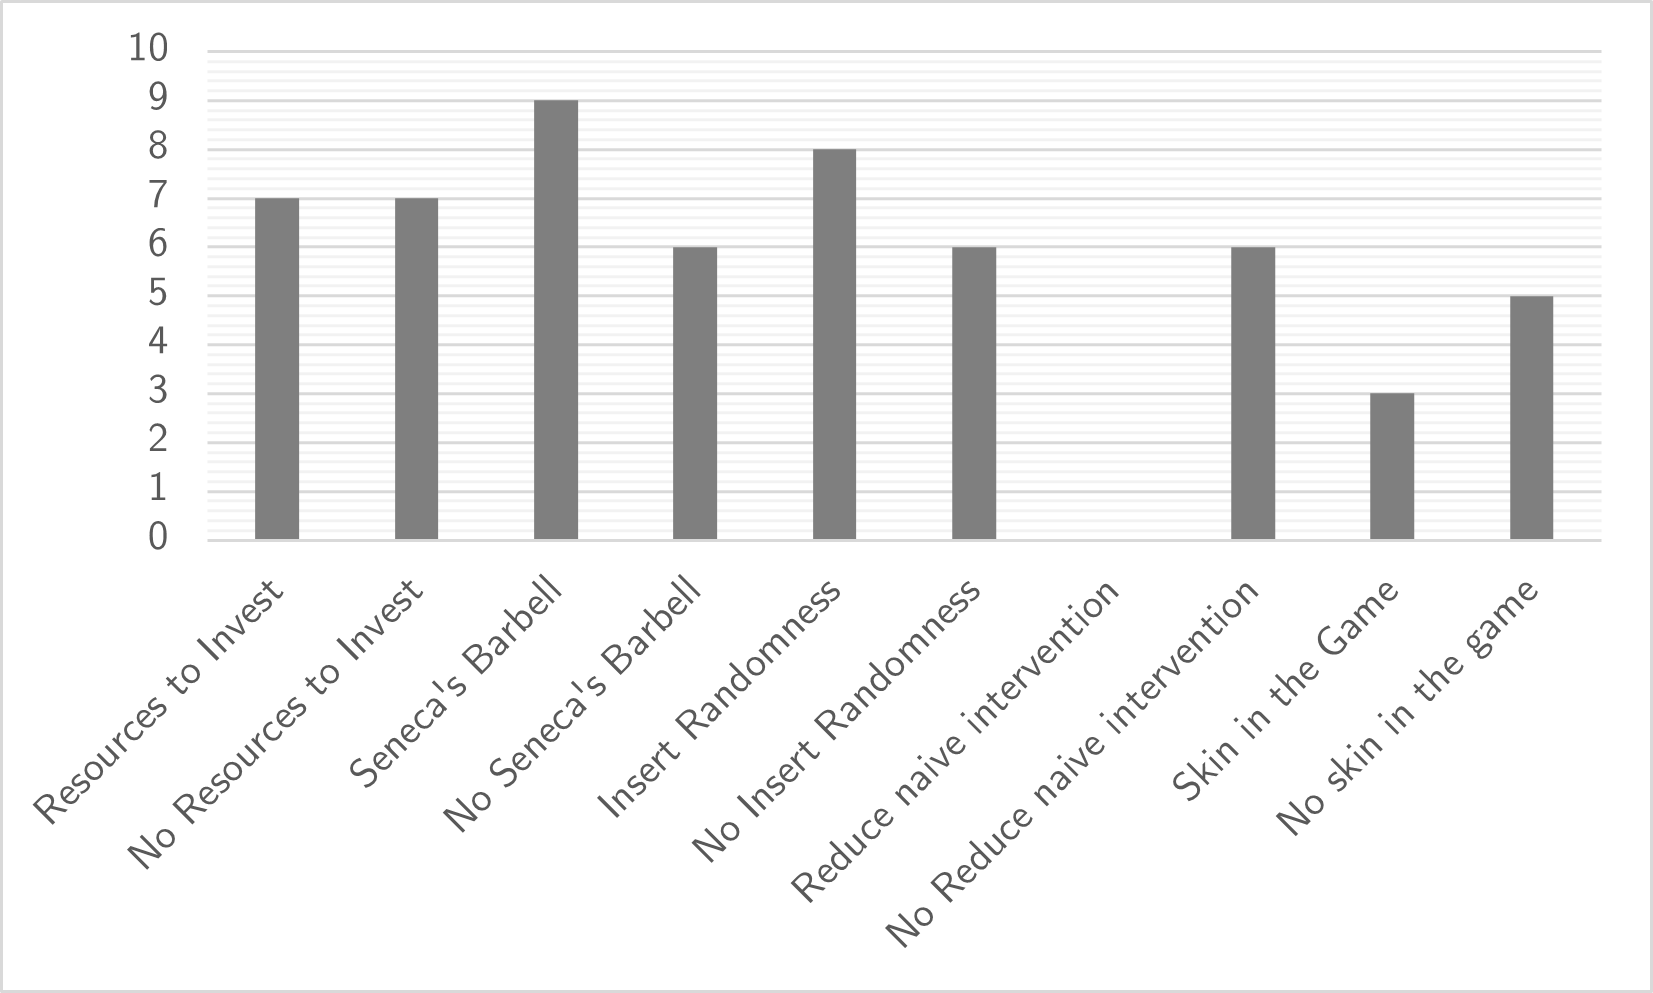
\includegraphics[width=0.95\linewidth]{images/antifragile_frequency}
		\caption{Antifragile Frequency}
		\label{fig:antifragilefrequency}
	\end{subfigure}%
	\begin{subfigure}[H]{0.5\textwidth}
		\centering
		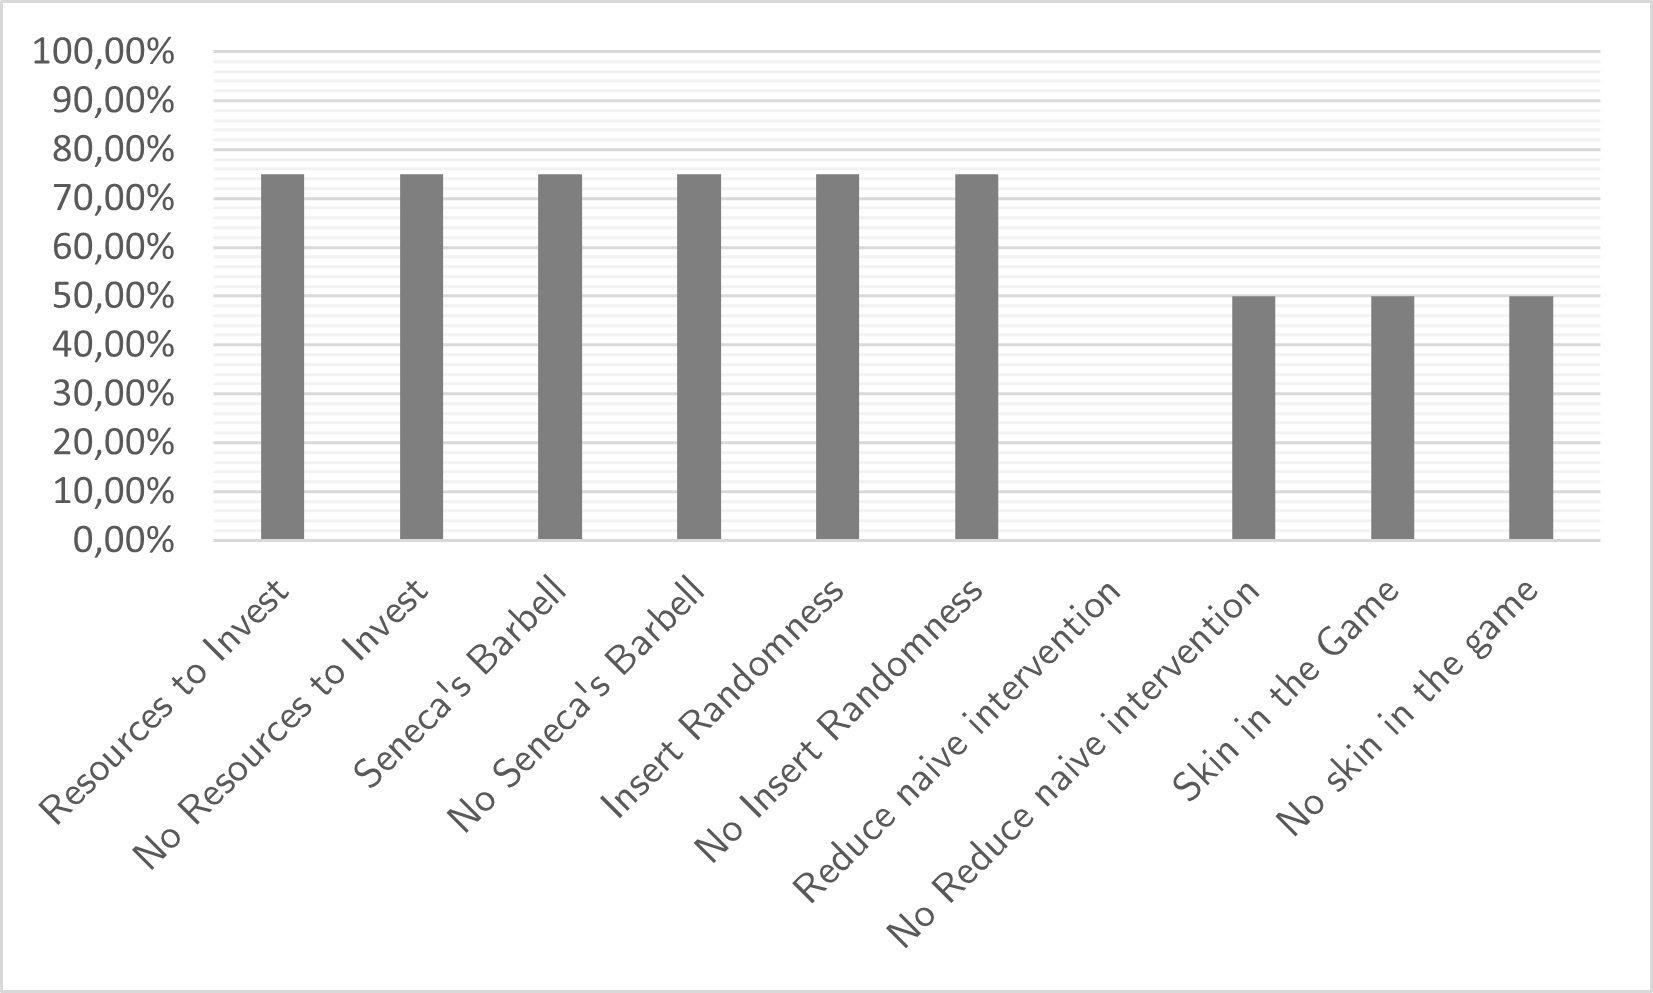
\includegraphics[width=0.95\linewidth]{images/antifragile_cases}
		\caption{Antifragile \% of Cases}
		\label{fig:antifragilecases}
	\end{subfigure}
	\caption{Interview results Antifragile}
	\label{fig:interviewresultsantifragile}
\end{figure}
\subsection{Learning organisation}
\begin{figure}[H]
	\centering
	\begin{subfigure}[H]{0.5\textwidth}
		\centering
		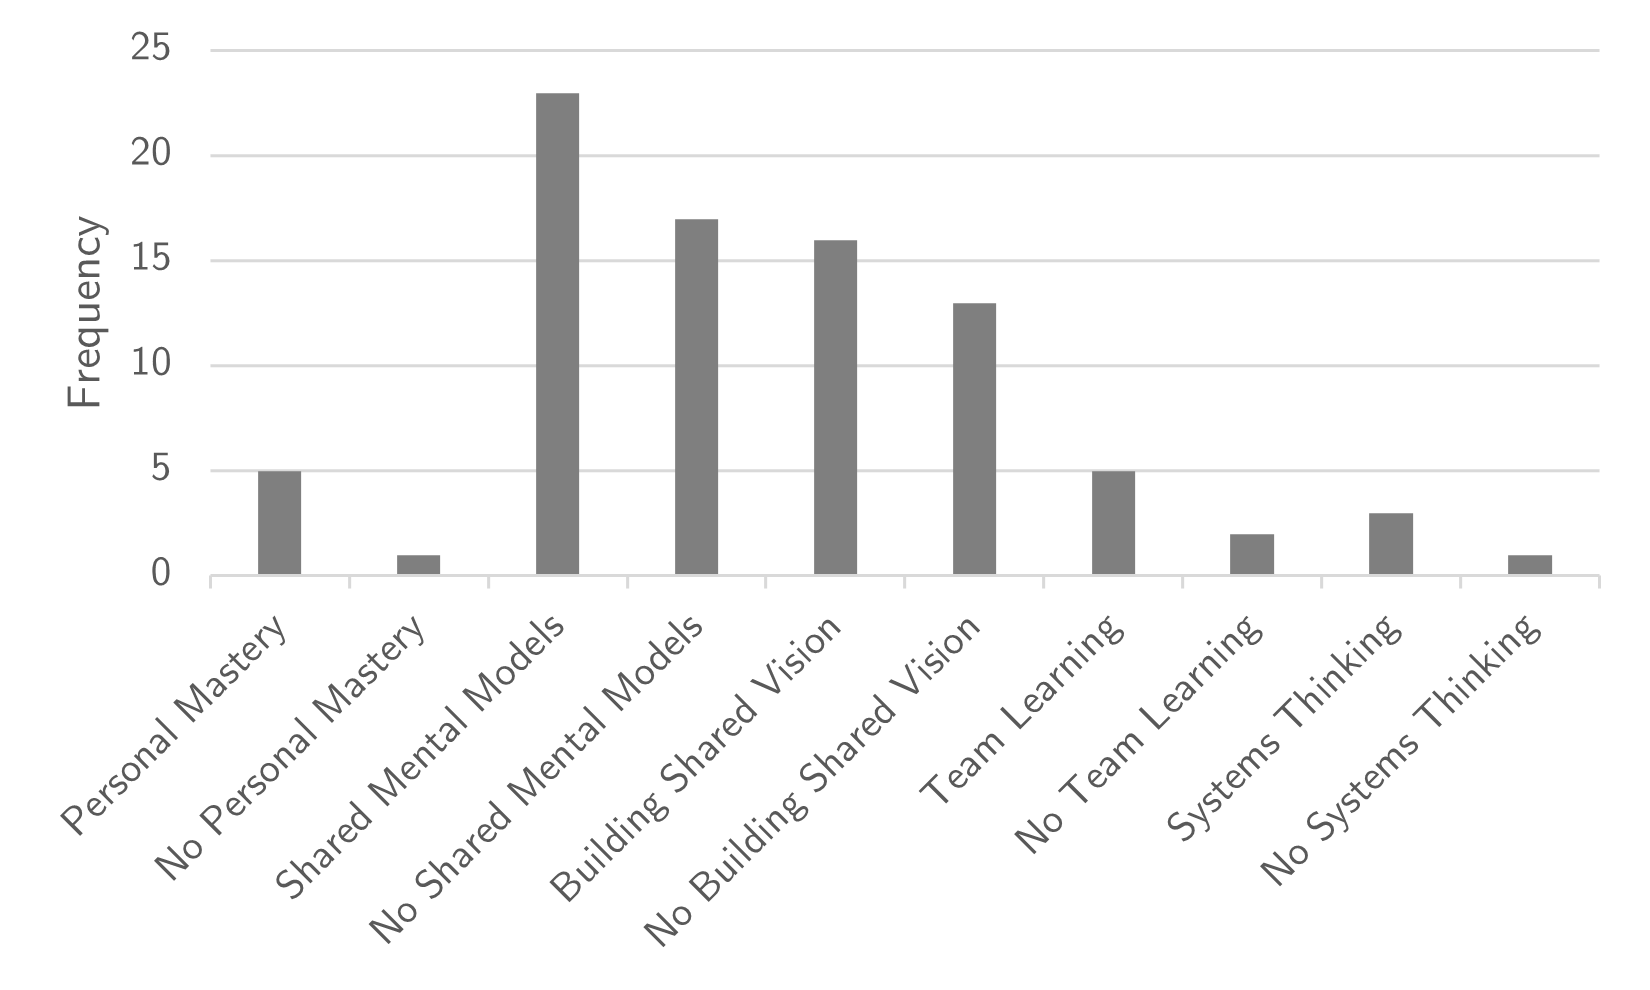
\includegraphics[width=0.95\linewidth]{images/learningorganisation_frequency}
		\caption{Learning Organisation Frequency}
		\label{fig:learningorganisationfrequency}
	\end{subfigure}%
	\begin{subfigure}[H]{0.5\textwidth}
		\centering
		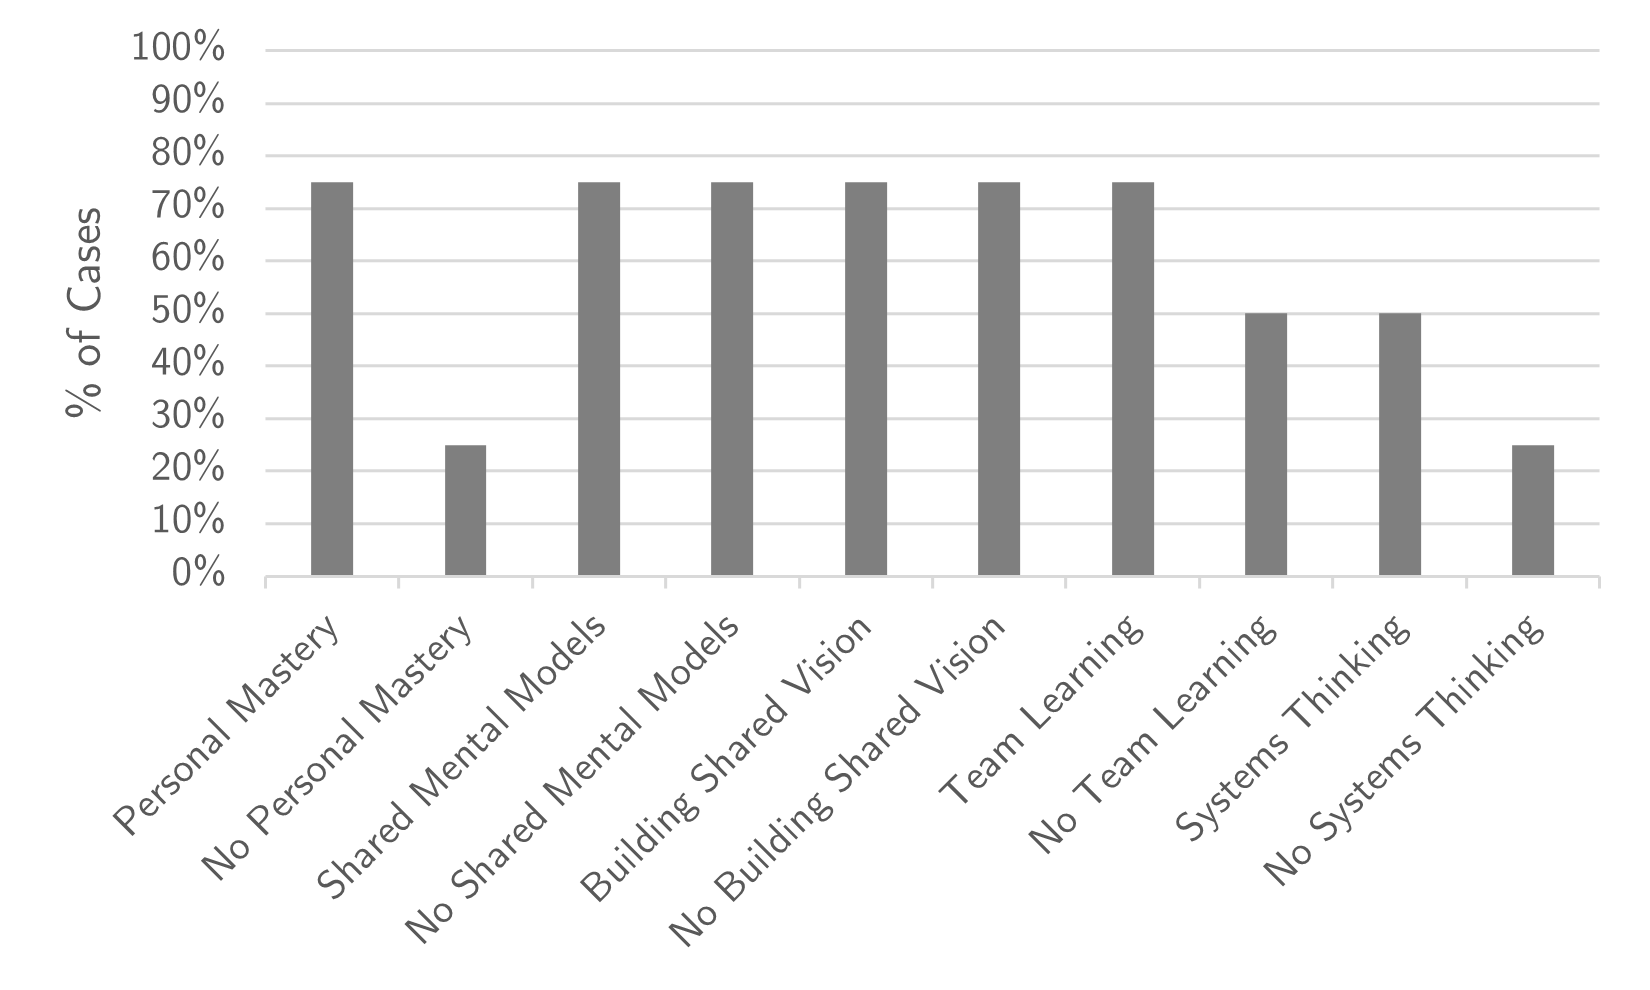
\includegraphics[width=0.95\linewidth]{images/learningorganisation_cases}
		\caption{Learning Organisation \% of Cases}
		\label{fig:learningorganisationcases}
	\end{subfigure}
	\caption{Interview results Learning Organisation}
	\label{fig:learningorganisationsantifragile}
\end{figure}


\subsection{Enterprise Architecture schools of thought}
\begin{figure}[H]
	\centering
	\begin{subfigure}[H]{0.5\textwidth}
		\centering
		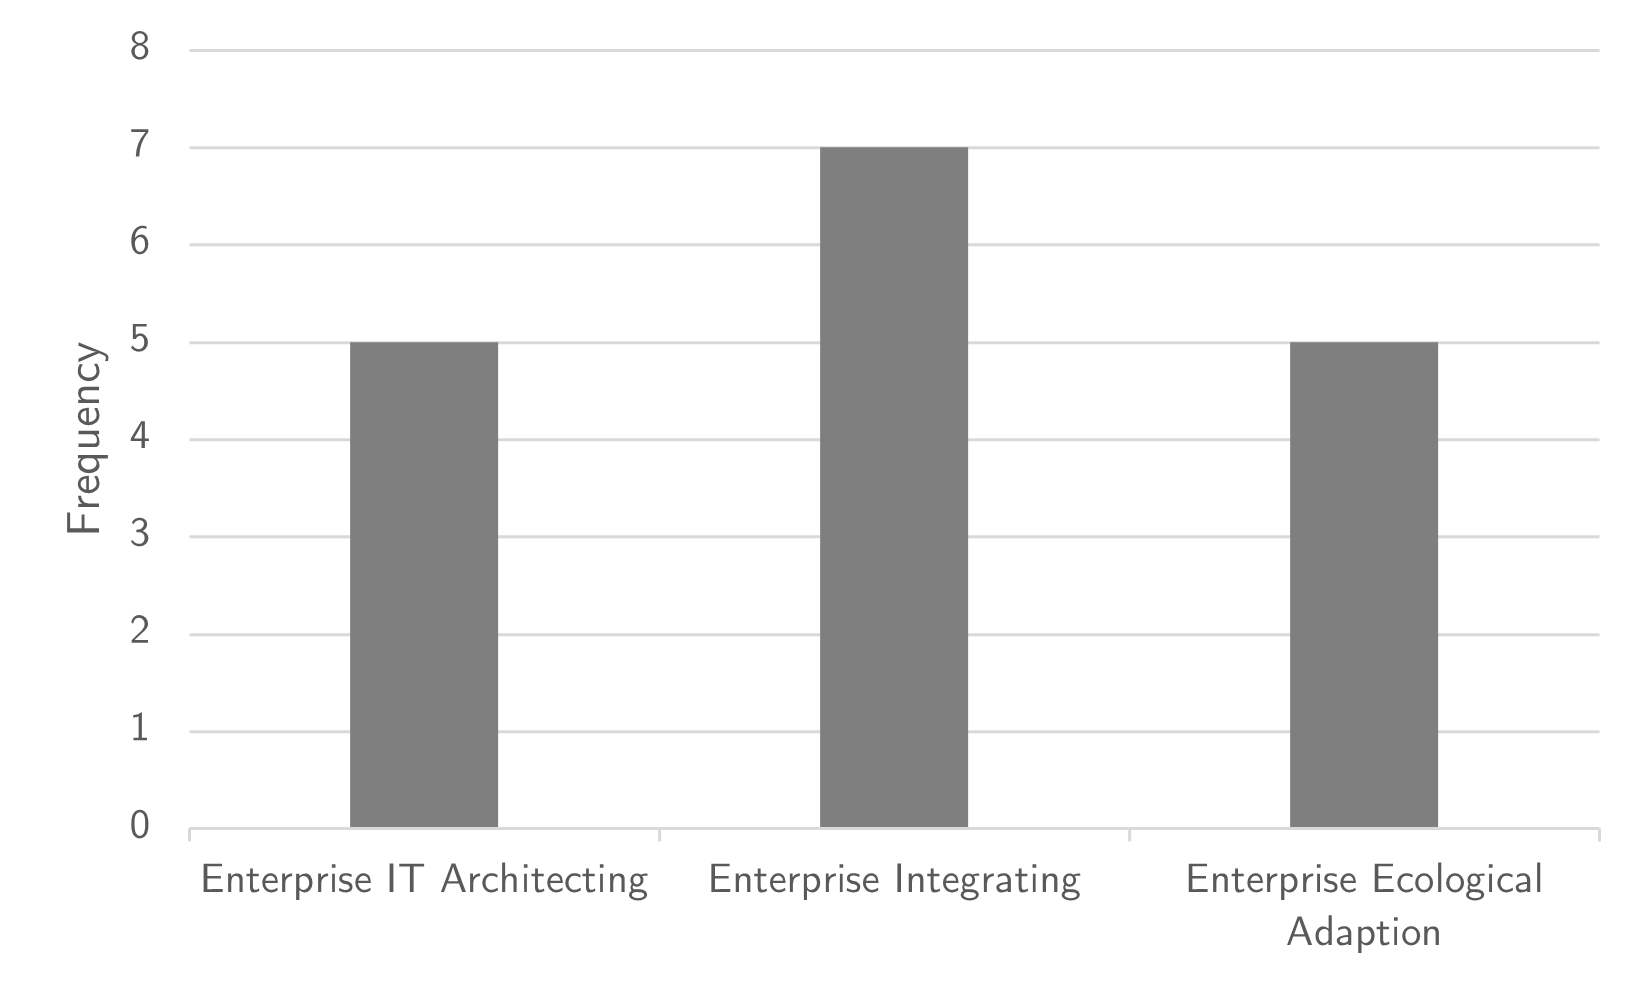
\includegraphics[width=0.95\linewidth]{images/easchools_frequency}
		\caption{Enterprise Architecture Schools of thought Frequency}
		\label{fig:easchoolsfrequency}
	\end{subfigure}%
	\begin{subfigure}[H]{0.5\textwidth}
		\centering
		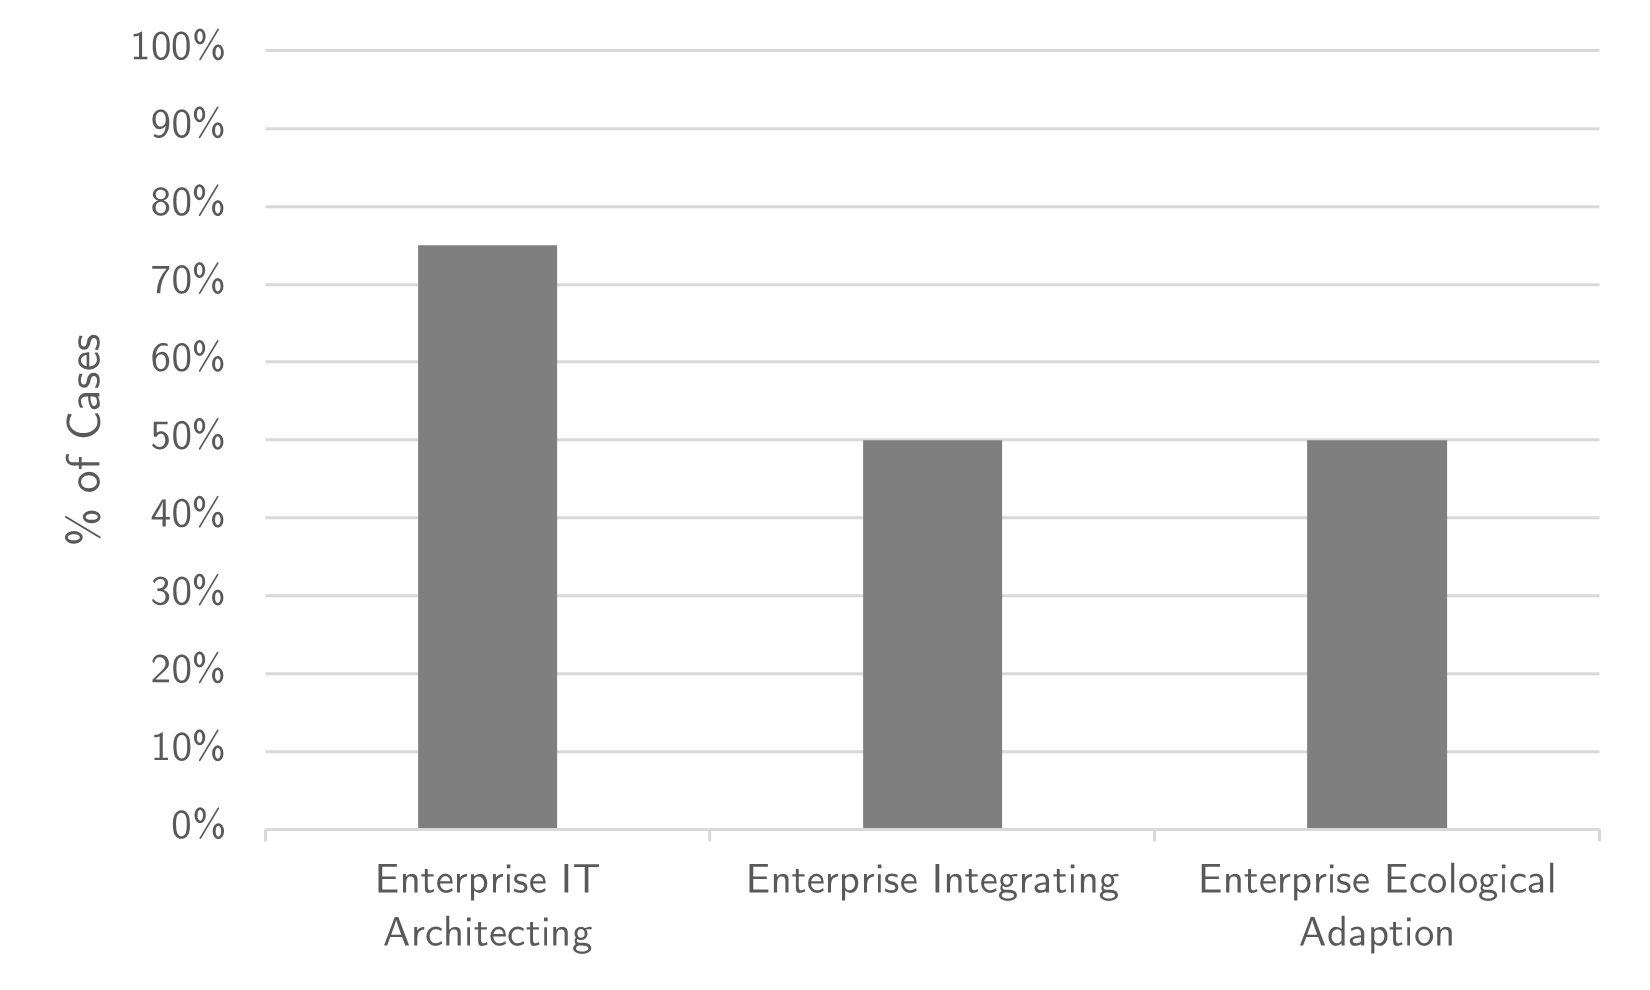
\includegraphics[width=0.95\linewidth]{images/easchools_cases}
		\caption{Enterprise Architecture Schools of thought \% of Cases}
		\label{fig:easchoolscases}
	\end{subfigure}
	\caption{Interview results Enterprise Architecture Schools of thought}
	\label{fig:easchoolsantifragile}
\end{figure}


\subsection{Findings}
\begin{figure}[H]
	\centering
	\begin{subfigure}[H]{0.5\textwidth}
		\centering
		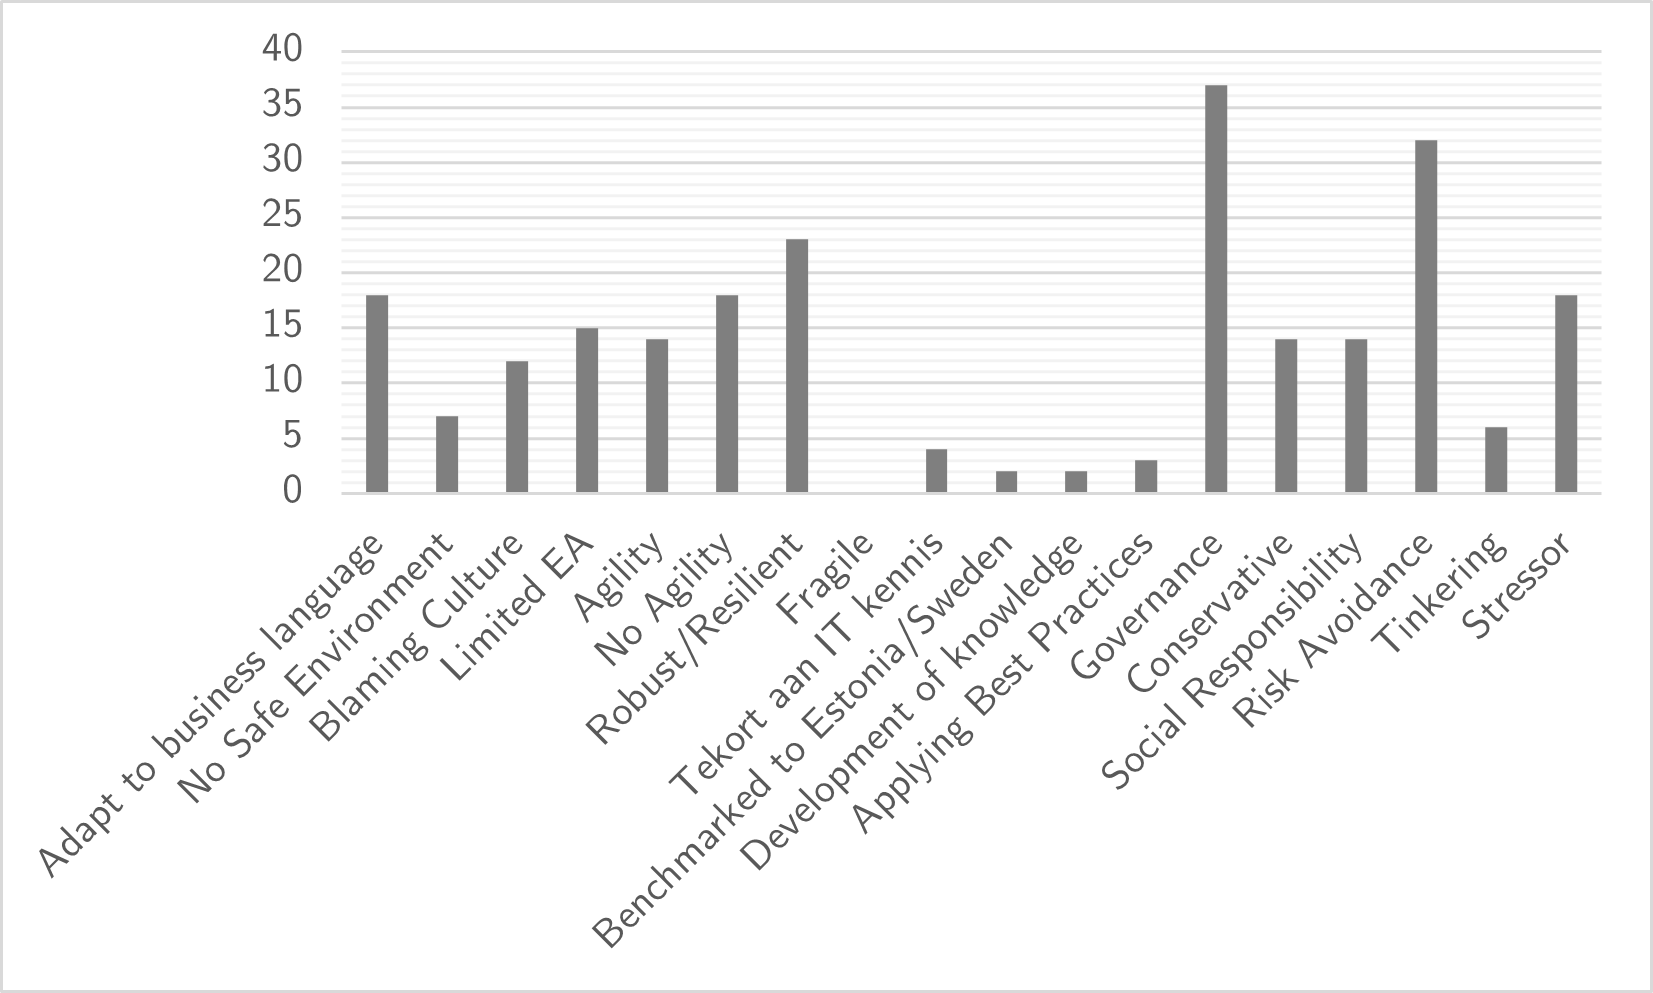
\includegraphics[width=0.95\linewidth]{images/findings_frequency}
		\caption{Findings Frequency}
		\label{fig:findingsfrequency}
	\end{subfigure}%
	\begin{subfigure}[H]{0.5\textwidth}
		\centering
		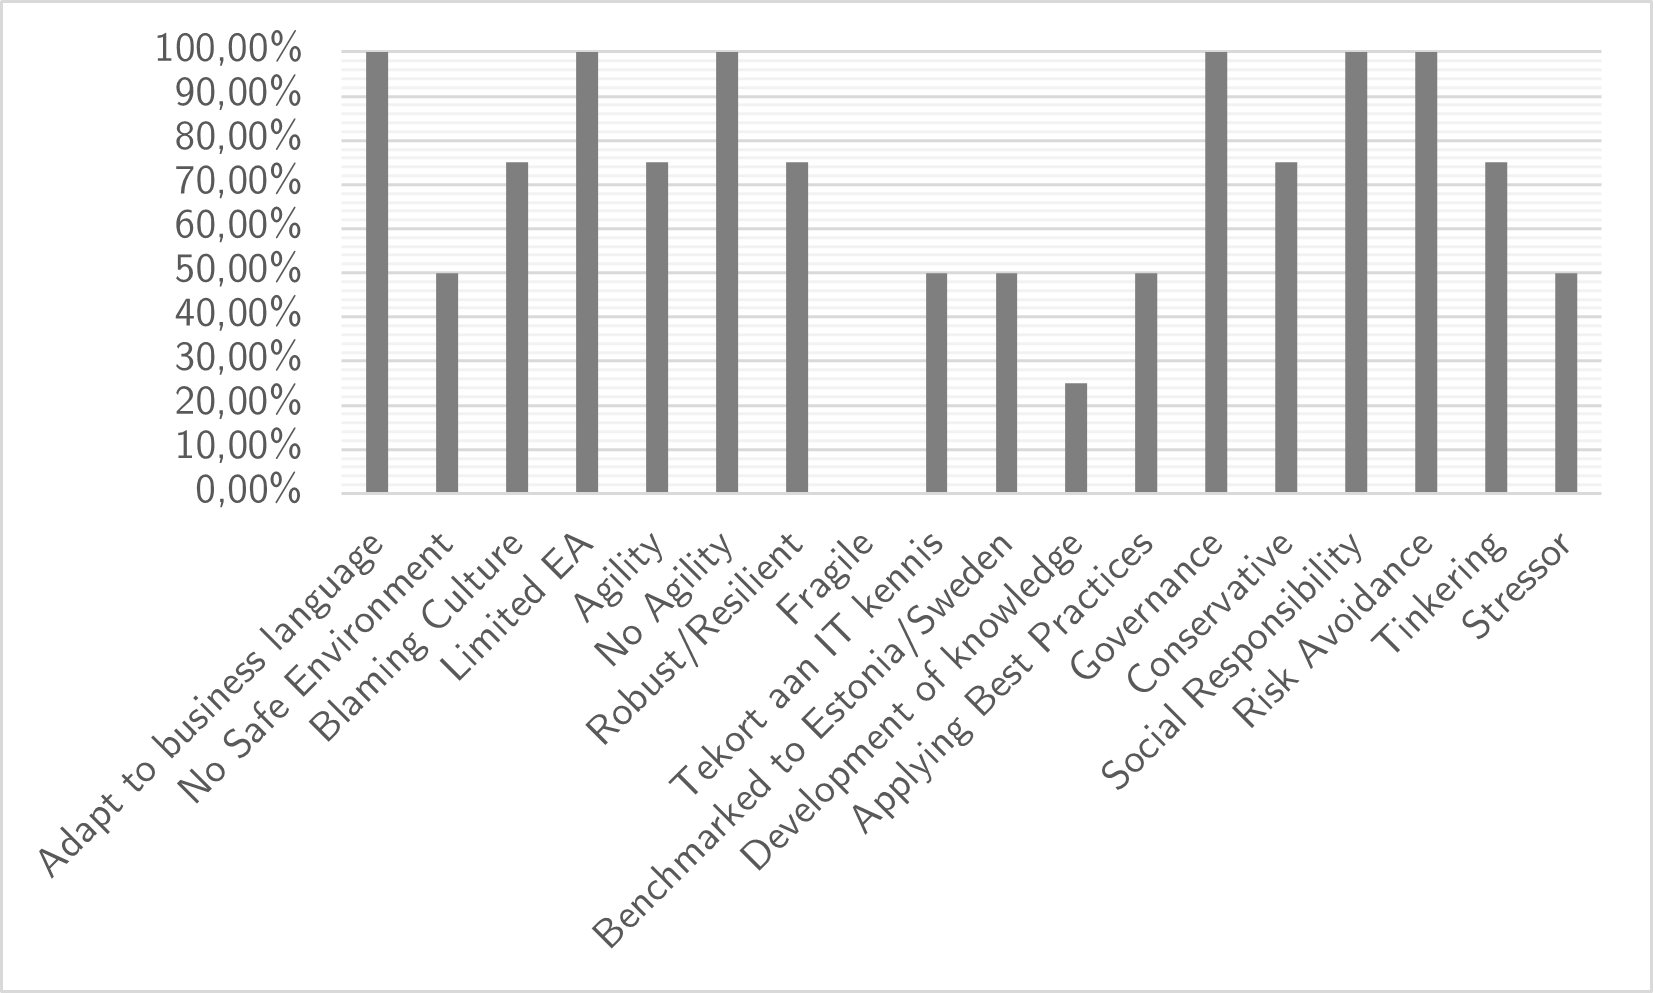
\includegraphics[width=0.95\linewidth]{images/findings_cases}
		\caption{Findings \% of Cases}
		\label{fig:findingscases}
	\end{subfigure}
	\caption{Interview results Findings}
	\label{fig:interviewresultsfindings}
\end{figure}


\section{Identified success factors}

\label{sec:interviewidentifiedsuccessfactors}
\begin{table}[!h]
	\begin{center}
		%\resizebox{\textwidth}{!}{%
			\begin{tabular}{@{}llllll@{}}
				%\toprule
				\textbf{Attribute} & \textbf{Behaviour} & \rot{90}{\textbf{Central Government}} & \rot{90}{\textbf{Local Government}} & \rot{90}{\textbf{Independent Software Vendor}} & \rot{90}{\textbf{Service Provider}} \\ \midrule
				Top Down C\&C & Engineering Resilience & \checkmark & \checkmark & \checkmark & \checkmark \\
				Micro-Management & Engineering Resilience & & & & \\
				Redundancy & Systems Resilience & & & & \\
				Modularity & Systems Resilience & & & & \\
				Loosely coupled & Systems Resilience & & & & \\
				Diversity & \acrshort{cas} Resilience & & & & \\
				Optionality & \acrshort{cas} Resilience & & & & \\
				Non-Monotonicity & \acrshort{cas} Resilience & & & & \\
				Emergence & \acrshort{cas} Resilience & & & & \\
				Self-Organisation & \acrshort{cas} Resilience & & & & \\
				Insert low-level stress & \acrshort{cas} Resilience & & & & \\
				Network-connections & \acrshort{cas} Resilience & & & & \\
				Fail Fast & \acrshort{cas} Resilience & & & & \\
				\Gls{resourcestoinvest} & Antifragile & & & & \\
				\Gls{senecabarbell} & Antifragile & & & & \\
				\Gls{insertrandomness} & Antifragile & & & & \\			
				\Gls{reducenaiveintervention} & Antifragile & & & & \\
				\Gls{skininthegame} & Antifragile & & & & \\
				\Gls{personalmastery} & Learning Organisation & & & & \\
				\Gls{sharedmentalmodels} & Learning Organisation & & & & \\
				\Gls{buildingsharedvision} & Learning Organisation & & & & \\
				\Gls{teamlearning} & Learning Organisation & & & & \\
				\Gls{systemsthinking} & Learning Organisation & & & & \\
				\bottomrule
			\end{tabular}
		%}
		\caption{Identified success factors from interviews}
	\end{center}
\end{table}

\section{Findings}

The central government is mostly robust and has a high risk aversion. With the administrative bodies of the local government the risk aversion is less and there is more insert low level stress. Because of this the local government is used to all the stressors and more antifragile.

\begin{remark}
Needs better description
\end{remark}				%	Interview results
	\chapter{Expert group}
\label{ch:expertgroup}
\setcounter{footnote}{0}
In \cref{ch:interviews}, the \glspl{attribute} were selected. The selected \glspl{attribute} are most likely to have a positive influence on \acrshort{ea} in achieving \gls{antifragility} in the \gls{ps}. These attributes are the result of literature study (\cref{ch:attributes}) and the qualitative analysis of interviews (\cref{ch:interviews}). The \glspl{attribute} still needed to be validated for \gls{triangulation} to work. An expert group validated these \glspl{attribute}. All of the expert group participants have experience with \acrshort{ea} and the \gls{ps}. A survey on experience was part of the expert group session (\cref{tab:experiencevalidationgroup}). The expert group participants were selected to balance the group. There was a balanced mix of participants from the central government, the local government, independent software vendors, service providers, and universities. Ten experts participated in the session.

The duration of the expert group session was 2 hours. The expert group session was online with Microsoft Teams and Meeting Wizard (a group support system). The session was recorded and transcribed. All participants gave their consent. The recording and transcription are not publicly available because they cannot be anonymised\footnote{The Antwerp Management School can request the recordings and transcriptions only for (re)accreditations and visitations to enable the Antwerp Management School to comply with statutory obligations. The recordings and transcriptions are kept for seven years after graduation before being deleted.}.
\begin{table}[H]
	\centering
	\begin{tabular}{p{.55\textwidth}ccc}
		\toprule
		\textbf{Question} & \textbf{Years} & \textbf{Variability} & \textbf{Abstains} \\
		\midrule
		How many years of experience do you have in the field of \acrlong{ea}? & 9,8 & 8\% & 0 \\%
		How many years have you worked as an (Enterprise) Architect? & 10,6 & 12\% & 0 \\%
		How many years of experience do you have in the field of complexity sciences (like \gls{antifragile})? & 7,4 & 16\% & 0 \\%
		How many years of experience do you have with the \gls{ps}? & 12,2 & 17\% & 0 \\%
		How many years of experience do you have with working in publicly-held organisations? & 10 & 16\% & 0 \\%
		How many years of experience do you have with working in privately-held organisations? & 17,2 & 21\% & 0 \\%
		\bottomrule
	\end{tabular}%
	\caption[The average experience of expert group participants]{The average experience of expert group participants}
	\label{tab:experiencevalidationgroup}%
\end{table}%
All the participants received information beforehand by email. This information contained the invite, the goal of the session, the agenda and all relevant definitions. Three recorded seminars given by Nassim Nicholas Taleb\footnote{\url{https://www.youtube.com/watch?v=B2-QCv-hChY}, \url{https://www.youtube.com/watch?v=1NXaafTpVjM}, and \url{https://www.youtube.com/watch?v=C40zwpdc_yo}} were shared to ensure that the participants had a basic understanding of \gls{antifragility}. All participants confirmed that they did see at least one of the videos. The book of \textcite{Taleb2012} was read by multiple participants. For the session the following agenda was used:
\begin{enumerate}
	\item{Introduction}
	\item{Survey on the experience of the participants\footnote{For the outcome of this survey see \cref{tab:experiencevalidationgroup}}}
	\item{Presentation on the results of the research up to now\footnote{\url{https://github.com/JRBliekendaal/master-thesis/blob/3666f93bb95308572722082393e684ba40caa5cb/datasets/expertgroup/validationsession.pdf}}}
	\item{Validation of attributes and EA schools of thought}
	\item{Survey on the relevance of the research}
\end{enumerate}
Meeting Wizard supported the surveys and validations. The data set of the surveys and validations is publicly available as a Microsoft Excel file in the public GitHub repository\footnote{\url{https://github.com/JRBliekendaal/master-thesis/blob/3666f93bb95308572722082393e684ba40caa5cb/datasets/expertgroup/dataset_expertgroup.xlsx}} of this research.
\section{Validation of attributes}
\label{sec:validationofattributes}
The two newly found attributes (\cref{sec:attributeslikelysf}) \textit{\gls{adapttobusinesslanguage}} and \textit{\gls{safeworkingenvironment}} were moved to the \gls{antifragile} \glspl{attribute} and \acrshort{ea} \glspl{attribute}. \textit{\Gls{safeworkingenvironment}} was moved to the \glspl{attribute} of \gls{antifragile} and \textit{\gls{adapttobusinesslanguage}} was moved to the \glspl{attribute} of \acrshort{ea}. 

A specific approach was taken to validate the \glspl{attribute}. Through brainstorming as a group, the participants could add new \glspl{attribute}. The new \glspl{attribute} were explained, discussed, combined and sorted. The participants rated every \gls{attribute} with a one for least likely and ten for most likely. There was a rating session for the \glspl{attribute} of \gls{antifragility} and \acrshort{ea} and there was a rating session for the \acrshort{ea} schools of thought. The participants rated the sets based on the following questions:
\begin{enumerate}
	\item{For the \glspl{attribute}: ''To what extent is the \gls{attribute} a success factor for \gls{antifragility} in the \gls{ps}?''}
	\item{For the \acrlong{ea} schools of thought: ''To what extent is the \acrlong{ea} school of thought a success factor for \gls{antifragility} in the \gls{ps}?''}
\end{enumerate}
\subsection{Validation of antifragile attributes}
\label{sub:validationofantifragileattributes}
While brainstorming, the participants came up with twelve possible new \glspl{attribute}. After discussion, only two remained. These two were \textit{'\gls{outsideincollaboration}'} and \textit{'\gls{datagovernanceplanes}'}. The others were the same as another \gls{attribute} or were a child of one of the other \glspl{attribute}. 
The expert group rated a total of nine \glspl{attribute}. As \cref{tab:validationofantifragileattributes} shows there are three \glspl{attribute} that had a variability of more than 50\%, and only two \glspl{attribute} scored less than a rating of 6. The new \glspl{attribute} were among those. There was one abstain on three \glspl{attribute}.
\begin{table}[H]
	\centering
	\begin{tabular}{p{.55\textwidth}ccc}
		\toprule
		\textbf{Attribute} & \textbf{Rating} & \textbf{Variability} & \textbf{Abstains} \\
		\midrule
		\Gls{optionality} & 6,9 & 32\% & 0 \\%
		\Gls{nonmonotonicity} & 7 & 51\% & 0 \\%
		\Gls{selforganisation} & 8,2 & 23\% & 0 \\%
		\Gls{failfast} & 7,8 & 35\% & 0 \\%
		\Gls{resourcestoinvest} & 6,7 & 36\% & 1 \\%
		\Gls{senecabarbell} & 5,8 & 37\% & 1 \\%
		\Gls{safeworkingenvironment} & 7,4 & 31\% & 0 \\%
		\Gls{outsideincollaboration} & 6,2 & 55\% & 0 \\%
		\Gls{datagovernanceplanes} & 4,4 & 56\% & 1 \\%
		\bottomrule
	\end{tabular}%
	\caption{Validation of antifragile attributes}
	\label{tab:validationofantifragileattributes}%
\end{table}%

\subsection{Validation of Enterprise Architecture schools of thought}
\label{sub:validationofeaschools}
Validating the \acrlong{ea} schools of thought needed a different approach. The presentation\footnote{\url{https://github.com/JRBliekendaal/master-thesis/blob/3666f93bb95308572722082393e684ba40caa5cb/datasets/expertgroup/validationsession.pdf}} introduced the attributes of \gls{antifragile} and \acrshort{ea}. The expert group could extend the list of \glspl{attribute} with new \glspl{attribute}. There is a high chance of influencing the expert group when presenting the most likely \acrlong{ea} school of thought. The approach was to use the expert group to validate the findings in a non-biased way. The validation used all three schools of thought. The expert group could rate the likelihood of the school of thought positively influencing \acrlong{ea} in achieving \gls{antifragility} in the \gls{ps}. 
\begin{table}[H]
	\centering
	\begin{tabular}{p{.55\textwidth}ccc}
		\toprule
		\textbf{School of thought} & \textbf{Rating} & \textbf{Variability} & \textbf{Abstains} \\
		\midrule%
		\Gls{enterpriseitarchitecting} & 5,6   & 34\%  & 0 \\
		\Gls{enterpriseintegrating} & 7,2   & 16\%  & 0 \\
		\Gls{enterpriseecologicaladaptation} & 8,8   & 27\%  & 0 \\
		\bottomrule%
	\end{tabular}%
	\caption[Rating of Enterprise Architecture schools of thought]{Rating of Enterprise Architecture schools of thought}
	\label{tab:validationgscoreeaschools}
\end{table}%
The rating had low variability, and no abstains (\cref{tab:validationgscoreeaschools}). \textit{\textit{\gls{enterpriseitarchitecting}}} had the lowest rating and \textit{\textit{\gls{enterpriseecologicaladaptation}}} had the highest with \textit{\textit{\gls{enterpriseintegrating}}} in between. It confirmed the results of the literature research (\cref{sub:eaapproaches}) and the interviews (\cref{sec:resultsofqda}).
\subsection{Validation of Enterprise Architecture attributes}
\label{sub:validationofenterprisearchitectureattributes}
The validation of the \acrshort{ea} \glspl{attribute} used the same approach like that of the \gls{antifragile} \glspl{attribute}. The validation contained the \acrlong{ea} school of thought of \gls{enterpriseecologicaladaptation} \glspl{attribute}. Brainstorming resulted in nine new identified \glspl{attribute}. After discussion, five remained. These five were \textit{\gls{agileenterprise}}, \textit{\gls{realtimetrust}}, \textit{\gls{fosterdialogue}}, \textit{\gls{architecturevalidation}} and \textit{\gls{alwaysfittingarchitecture}}. The expert group rated the the attributes.
\begin{table}[H]
	\centering
	\begin{tabular}{p{.55\textwidth}ccc}
		\toprule
		\textbf{Attribute} & \textbf{Rating} & \textbf{Variability} & \textbf{Abstains} \\
		\midrule
		\Gls{systeminenvironment} & 7,7   & 28\%  & 0 \\
		\Gls{holisticsystemicstance} & 7     & 47\%  & 0 \\
		\Gls{organisationallearning} & 7,3   & 44\%  & 0 \\
		\Gls{environmentallearning} & 7,7   & 29\%  & 0 \\
		\Gls{intraorganisationalcoherency} & 6,4   & 31\%  & 0 \\
		\Gls{systeminenvironmentcoevolutionlearning} & 6,6   & 36\%  & 0 \\
		\Gls{adapttobusinesslanguage} & 7,1   & 35\%  & 0 \\
		\Gls{agileenterprise} & 6,4   & 50\%  & 0 \\
		\Gls{realtimetrust} & 5,6   & 54\%  & 1 \\
		\Gls{fosterdialogue} & 6,9   & 32\%  & 0 \\
		\Gls{architecturevalidation} & 7,4   & 24\%  & 0 \\
		\Gls{alwaysfittingarchitecture} & 5,8   & 46\%  & 1 \\
		\bottomrule
	\end{tabular}%
	\caption[Rating of Enterprise Architecture attributes]{Rating of Enterprise Architecture attributes}
	\label{tab:validationofeaattributes}%
\end{table}%
The rating (\cref{tab:validationofeaattributes}) shows that two \glspl{attribute} have a variability of 50\% or higher, and only one \gls{attribute} got a rating of less than 6. All three were from the five new \glspl{attribute} from the expert group. There were only two abstains on a total of two attributes.
\section{Relevance of the research}
\label{sec:relevanceofresearch}
The final part of the expert group session was about the relevance of the research. A survey determined the research's relevance. The expert group rated the research on different areas of application. These areas of relevance were, \textit{in general}, \textit{for themselves}, \textit{for the public sector} and \textit{for the organisation of the expert}. The last question asked was if the expert group session fulfilled their expectations.

The variability of the ratings was low. There was only one abstain on the relevance of the research for the public sector. The question that scored the least was about the relevance for the organisation of the expert. The expert group finds the research relevant. They rated it with a rating of 8,2 (\cref{tab:relevanceofresearch}).
\begin{table}[H]
	\centering
	\begin{tabular}{p{.55\textwidth}ccc}
		\toprule
		\textbf{Question} & \textbf{Rating} & \textbf{Variability} & \textbf{Abstains} \\
		\midrule
		To what extent do you find the research relevant? & 8,2 & 23\% & 0 \\%
		To what extent did this session fulfil your expectations? & 8 & 24\% & 0 \\%
		To what extent do you think that the research can be used by yourself? & 7,7 & 10\% & 0 \\%
		To what extent do you think that the research can be used in the public sector? & 7,2 & 32\% & 1 \\%
		To what extent do you think that the research can be used by your organisation? & 6,6 & 33\% & 0 \\%
		\bottomrule
	\end{tabular}%
	\caption[Rating of the relevance of the research]{Rating of the relevance of the research}
	\label{tab:relevanceofresearch}%
\end{table}%				%	Add expert group chapter
	\include{contents/analysis}					%	Add Analysis Chapter
	\chapter{Conclusion and discussions}
\label{ch:conclusionanddiscussions}

\parencite{Dietz2008} and \parencite{Dietz2013}\\
\parencite{Digitaleoverheid2021}\\
\parencite{Knops2021}\\

\section{Conclusion}
\label{sec:conclusion}
We conducted literature research to answer the sub-questions. What is the Dutch \gls{ps}? What is \gls{antifragile}, and what are possible success factors for \gls{antifragility}? What is \acrlong{ea}, and what are the possible success factors of \acrlong{ea}? We presented the answers to these questions in the background chapter (\cref{ch:theoreticalbackground}) of this thesis. The literature research delivered us a list of \textit{twenty-three} generic attributes of \gls{antifragile} and \textit{six} generic \glspl{attribute} of \acrlong{ea} that can positively influence achieving \gls{antifragility} with \acrlong{ea}.

Following this, we conducted interviews with \glspl{cxo} from the Dutch public sector (\cref{ch:interviews}) and an expert group composed of (Enterprise) Architects from the Dutch \gls{ps} (\cref{ch:expertgroup}) to determine which of those \glspl{attribute} are applicable to the Dutch \gls{ps}. We performed a \acrlong{qda} on the data set of the interviews, and we used a Group Support System for the expert group. The Group Support System provided us with the necessary tools and helped us capture the findings. 

We combined the literature study results, interviews, and expert group for \gls{triangulation}. We analysed the \glspl{attribute} on the occurrence of the \glspl{attribute} in all three research tools (\cref{app:combinedfindings}). If an \gls{attribute} occurred in all three research tools, we decided that this \gls{attribute} is \textit{most likely} a success factor for the Dutch \gls{ps}. When an \gls{attribute} occurred in two out of three research tools, we decided that this \gls{attribute} is \textit{likely} a success factor for the Dutch \gls{ps} but it needs more research to determine this. \Glspl{attribute} that occurred in only one of the three research tools are least likely to be a success factor for the Dutch \gls{ps}.

{\small\tabcolsep=3pt  % hold it local
\begin{longtable}{@{}p{0.2\textwidth}p{0.15\textwidth}p{0.6\textwidth}@{}}
	\textbf{Attribute} & \textbf{Category} & \textbf{Definition} \\%
	\midrule%
	\endhead%
	\hline
	\endfoot%
	\caption[Most likely success factors]{Most likely success factors}
	\label{tab:identifiedsuccessfactors}
	\endlastfoot%
	\Gls{optionality} & \Gls{antifragile} & \Glsdesc*{optionality} \\%
	\Gls{failfast} & \Gls{antifragile} & \Glsdesc*{failfast} \\%
	\Gls{resourcestoinvest} & \Gls{antifragile} & \Glsdesc*{resourcestoinvest} \\%
	\Gls{systeminenvironment} & \acrlong{ea} & \Glsdesc*{systeminenvironment} \\%
	\Gls{environmentallearning} & \acrlong{ea} & \Glsdesc*{environmentallearning} \\%
	\Gls{intraorganisationalcoherency} & \acrlong{ea} & \Glsdesc*{intraorganisationalcoherency} \\%
	\Gls{systeminenvironmentcoevolutionlearning} & \acrlong{ea} & \Glsdesc*{systeminenvironmentcoevolutionlearning} \\%
		\bottomrule%
\end{longtable}%
}
{\small\tabcolsep=3pt  % hold it local
\begin{longtable}{@{}p{0.2\textwidth}p{0.15\textwidth}p{0.6\textwidth}@{}}
	\textbf{Attribute} & \textbf{Category} & \textbf{Definition} \\%
	\midrule%
	\endhead%
	\hline
	\endfoot%
	\caption[Likely success factors]{Likely success factors}
	\label{tab:identifiedpossiblefactors}
	\endlastfoot%
	\Gls{nonmonotonicity} & \Gls{antifragile} & \Glsdesc*{nonmonotonicity} \\%
	\Gls{selforganisation} & \Gls{antifragile} & \Glsdesc*{selforganisation} \\%
	\Gls{senecabarbell} & \Gls{antifragile} & \Glsdesc*{senecabarbell} \\%
	\Gls{safeworkingenvironment} & \Gls{antifragile} & \Glsdesc*{safeworkingenvironment} \\%
	\Gls{holisticsystemicstance} & \acrlong{ea} & \Glsdesc*{holisticsystemicstance} \\%
	\Gls{organisationallearning} & \acrlong{ea} & \Glsdesc*{organisationallearning} \\%
	\Gls{adapttobusinesslanguage} & \acrlong{ea} & \Glsdesc*{adapttobusinesslanguage} \\%
	\bottomrule%
\end{longtable}%
}
\begin{remark}
	Do not forget. \Gls{adapttobusinesslanguage} and \gls{safeworkingenvironment} are special. These were not found in literature. So these can be differentiators especially for the Dutch public sector!!!!! This needs more research!
\end{remark}




\section{Discussions}
\label{sec:discussions}

\begin{itemize}
	\item{Discuss the definition of System Thinking vs Emergence}
	\item{Discuss Blaming Culture Public Sector}
	\item{Discuss Speaking the language of the Business with EA}
	\item{Discuss is the public sector really different from that of the private sector?}
	\item{Discuss is the Dutch public sector different than that from other countries?}
\end{itemize}

\subsection{Is the public sector in The Netherlands unique?}
\label{sub:discussionpublicsector}
Is the public sector in The Netherlands the same as in the rest of the world? This needs further research and needs to be confirmed so that the outcome of this research is universally applicable. Maybe the outcome can be generalised. Further research should demonstrate this.

\subsection{Is the public sector different then the private sector?}
\label{sub:discussionpublicvsprivate}


\subsection{Size of Expert Group}
\label{sub:discussionsizeofeg}
Is the size of the delphi group large enough to determine....
\subsection{The composition of the Expert Gropu}
\label{sub:compositionofeg}
Is the composition of the Delphi Group a good reflection of the Public Sector Market?

\subsection{enterprise archiecture}

agree to disagree. less know than expected. different viewpoints. different schools, opinions, practices, etc.. LIterature study did not help and made it even worse.

\subsection{Causal Loop Diagram}

\section{Recommendations}
\label{sec:reccomandations}

\begin{itemize}
	\item{Research not on the public sector but only parts of the public sector}
\end{itemize}				%	Add the conclusion
	\chapter{Retrospective}
\label{ch:retrospective}
\lipsum[1]

\begin{itemize}
	\item{The added value of a Co-Promotor}
\end{itemize}
			%	Add the restrospective
	
	% Tail of Thesis

	\printbibliography[title={References}]			%	Add Bibliography
	\newpage										%
	\addcontentsline{toc}{chapter}{List of Figures} % Add List of Figures to Table of Contents
	\listoffigures									%	Add the List of Figures
	\newpage										%			
	\addcontentsline{toc}{chapter}{List of Tables} 	% Add List of Tables to Table of Contents
	\listoftables									%	Add the list of Tables
	\printglossary[title=Glossary of Terms] 		% Add Glossary of Terms
	\printglossary[type=\acronymtype,title=Abbreviations] % Add Abbreviations
	
	\begin{appendices}	% Add Appendices
%		\chapter{Personal Motivation}
I always want to know how something works and why it works the way it works. This eagerness started at a very early age. I always demolished birthday presents into their parts. I wondered how things worked, and I did not stop with the research on the how and why until I understood it. The search for the how and why is a central theme in my life. And because of this, I never stopped learning. When the why is not known, I never give up researching—not knowing the why has only the meaning that nobody has found the answer yet. 

My essential attitude is that of a mathematician or a scientist. I am very binary and sceptical when something is somewhere in between, and I am not fond of shades of grey. So clear definitions is what I pursue. Everything needs an explanation. When I cannot explain, I do not fall back to religion, infinity, approximately, or even ''it is just what it is''. I only accept that we did not find the answer yet.

This journey started with simple things like a toy car or a doll that had a mechanism of saying things. I still think of my little sister, who found hers back in tiny pieces. Later the subjects of research began to be different. Secondary education drove me to understand chemistry, physics, and biology, and I needed an explanation on the who and why to understand it. This drive was probably the main reason I was not perfect in languages. You cannot put consistent rules on languages.  Languages do not have a clear rationale for the rules, and I often heard it is just the way it is.

Grammar school taught me that I was a natural in research, and I decided to pursue research. Firstly at several Universities, but I failed big time. The Universities at that time gave me a lot of answers that it is the way it is, and most of the lecturers did not appreciate me challenging them on the why. Because of this, I started pursuing a job that could fulfil my eagerness for researching, and I found that with an IT Company in the Netherlands.

The technical (hard) side of IT was, at that time, a match made in heaven. Most of the time, it is just like math, you have a clear answer, and you know why you get that answer. Before I knew it, I was a Senior Consultant and an IT Architect shortly after that. Gaining knowledge is one thing that drives me, but the other thing is sharing that knowledge with others. Gaining and sharing knowledge is the thing that gets me up in the morning. For sharing knowledge, I taught, as a trainer, adults on the why and how of technology subjects for years.

In those years, I advised dozens of companies of the public and private sectors in the Benelux on how they could apply technologies and what problem it solved for them. This period did teach me a lot by seeing other companies and working with different kinds of people. But technology was driving me less and less, and I became aware that technology was only a means to reach a (business) goal. I often solved my customers' problems by not introducing new technology but changing their processes, information architecture, culture, team compositions, or organisational construction. I became more and more interested in how and why organisations could achieve their goals by using IT.


Personal story

Why this subject

Road to this subject

Personal motivation

Personal goals
		\appendix
\chapter{Properties of the Enterprise Architecture schools of thought}
\label{app:easchoolsproperties}
This appendix describes the Enterprise Architecture school of thoughts in more details. It will help the reader with detailed understanding of the three schools of thought.
\section{The properties of Enterprise IT Architecting}
The school of thought \gls{enterpriseitarchitecting} \parencite[p. 39]{Lapalme2012} is summarised in the following table.
\begin{table}[!h]
	\begin{center}
		\resizebox{\textwidth}{!}{%
			\begin{tabular}{@{}p{.2\textwidth}p{.8\textwidth}@{}}
				\toprule%
				& \textbf{\gls{enterpriseitarchitecting} school of thought} \\%
				\midrule%
				Motto    		& Enterprise architecture is the glue between business \& IT \\
				Objectives and 	& Effectively enable the enterprise strategy \\
				concerns		& Support IT planning and reduce cost \\
				& Enable business \\
				Principles and  & Apply reductionist (mechanistic) stance \\
				assumptions		& Don't question business strategies  \\
				& Design organisational dimensions independently \\
				& Don't worry about non-IT dimensions; they are not your concerns \\
				Skills 			& Have technical competence and engineering knowledge \\
				Challenges		& Convince the organisation to accept the designed plans \\
				Insights		& Permits the design of robust and complex technological solutions \\
				& Fosters the creation of high-quality models and planning scenarios \\
				Limitation		& Can produce inadequate or unfeasible solutions for the larger organizational context \\
				& Struggles with solution acceptance and implementation barriers \\
				& Susceptible to “perfect” designs 	that support unsustainable strategies \\
				\bottomrule%
			\end{tabular}
		}
		\caption{Properties of \gls{enterpriseitarchitecting}}
		\label{tab:enterpriseitarchitecting}	
	\end{center}
\end{table}
\newpage
\section{The properties of Enterprise Integrating}
The school of thought \gls{enterpriseintegrating} is summarised in the following table.
\begin{table}[!h]
	\begin{center}
		\resizebox{\textwidth}{!}{%
			\begin{tabular}{@{}p{.2\textwidth}p{.8\textwidth}@{}}
				\toprule%
				& \textbf{\gls{enterpriseintegrating} school of thought} \\%
				\midrule%
				Motto    		& Enterprise Architecture is the link between strategy and execution \\
				Objectives and 	& Effectively implement the enterprise strategy \\
				concerns		& Support organizational coherence \\
				Principles and  & Apply a holist (systemic) stance \\
				assumptions		& Don’t question business strategies and objectives  \\
				& Manage the environment \\
				& Jointly design all organisational dimensions \\
				Skills 			& Facilitate small-group collaboration \\
				& Apply systems thinking \\
				Challenges		& Understand organizational systemic dynamics \\
				& Collaborate across the organization \\
				& Encourage systems thinking and paradigm shifts \\
				Insights		& Permits the design of comprehensive solutions \\
				& Enables significant organizational efficiency by eliminating unnecessary contradictions and paradoxes \\
				Limitation		& Susceptible to “perfect” designs that support unsustainable strategies \\
				& Requires a paradigm shift from reductionism to holism \\
				\bottomrule%
			\end{tabular}
		}
		\caption{Properties of \gls{enterpriseintegrating}}
		\label{tab:interpriseintegrating}	
	\end{center}
\end{table}
\newpage
\section{The properties of Enterprise Ecological Adaptation}
\label{appsec:eea}
The school of thought \acrlong{eea} is sumarised in the following table.
\begin{table}[!h]
	\begin{center}
		\resizebox{\textwidth}{!}{%
			\begin{tabular}{@{}p{.2\textwidth}p{.8\textwidth}@{}}
				\toprule%
				& \textbf{\gls{enterpriseecologicaladaptation} school of thought} \\%
				\midrule%
				Motto    		& \acrshort{ea} is the means for organizational innovation and sustainability \\
				Objectives and 	& Innovate and adapt    \\
				concerns		& Support organizational coherence \\
				& Encourage \acrlong{sie} coevolution \\
				Principles and  & Apply a holist (systemic) stance \\
				assumptions		& \acrlong{sie} coevolution  \\
				& Environment can be changed \\
				& Jointly design all organisational dimensions \\
				Skills 			& Foster dialogue \\
				& Apply system and \acrlong{sie} thinking \\
				& Facilitate larger-group collaboration \\
				Challenges		& Foster sensemaking \\
				& Encourage systems thinking and \acrlong{sie} paradigm shifts \\
				& Collaborate across the organisation \\
				Insights		& Fosters \acrlong{sie} coevolution and enterprise choherency \\
				& Fosters organisational innovation and sustainability \\
				Limitation		& Requires many organisational preconditions for management and strategy creation \\
				\bottomrule%
			\end{tabular}
		}
		\caption{Properties of \gls{enterpriseecologicaladaptation}}
		\label{tab:eaeea}	
	\end{center}
\end{table} % Add EA Schools of thought of Lapalme details
		%\appendix
\chapter{Authors of the Enterprise Architecture schools of thought}
\label{app:easchoolsresearchers}
This appendix indicates which authors in the \acrlong{bok} are related to which school of thought. \textcite[p. 42]{Lapalme2012} mapped enterprise architecture authors from the \acrlong{bok} according to the three schools of thought.
\begin{table}[!h]
	\begin{center}
		\resizebox{\textwidth}{!}{%
			\begin{tabular}{@{}p{.33\textwidth}p{.33\textwidth}p{.33\textwidth}@{}}
				\toprule%
				\textbf{\gls{enterpriseitarchitecting}} & \textbf{\gls{enterpriseintegrating}} & \textbf{\gls{enterpriseecologicaladaptation}} \\%
				\midrule%
				Clive Finkelstein				&		Peter Bernus and Colleagues (editors)	&		Jamshid Gharajedaghi \\%
				Inge Hanschke					&		Ronald Giachetti						&		Tom Graves \\%
				Col Perks and Tony Beveridge	&		Leon Kappelman (editor)					&		Jan Hoogervorst \\%
				Jeanne Ross and colleagues		&		Martin Op't Land and colleagues			&		James Martin \\%
				Steven Spewak and Steven Hill	&												&		Kevin Smith and Tom Graves \\%
				Martin van den Berg and Marlies van Steenbergen & 								&		James Lapalme and Donald de Guerre \\%
				\bottomrule%
			\end{tabular}
			}
		\caption{Authors of the Enterprise Architecture schools of thought}
		\label{tab:easchoolresearchers}	
	\end{center}
\end{table} % Add writers per school of thought of Lapalme
%		\chapter{Overview of Laws}
\setcounter{footnote}{0}
The research references to several laws. This appendice gives a small explainatory overview of these laws.

\begin{itemize}
	\item{2\textsuperscript{nd} Law of Thermodynamics}
	\item{Conways Law}
	\item{Metcalfe's Law}
	\item{Law of Municipalities}
\end{itemize}

\section{2\textsuperscript{nd} Law of Thermodynamics}
\label{sec:appendix2ndlawthermodynamics}
The ‘2\textsuperscript{nd} Law’ was formulated after nineteenth century engineers noticed that heat cannot pass from a colder body to a warmer body by itself. It states that in any closed system the amount of order can never increase, only decrease over time. Another way of saying this is that entropy always increases.

\section{Conway's Law}
Any organization that designs a system (defined broadly) will produce a design whose structure is a copy of the organization's communication structure.

\section{Metcalfe's Law}
Metcalfe's Law\footnote{\url{https://www.techopedia.com/definition/29066/metcalfes-law}} states that a network's impact is the square of the number of nodes in the network. For example, if a network has 10 nodes, its inherent value is 100 (10 * 10). The end nodes can be computers, servers and/or connecting users.

\section{Thorbecke's Law}

\section{Lehman's Law of Increasing Complexity}
As an evolving program is continually changed, its complexity, reflecting deteriorating structure, increases unless work is done to maintain or reduce it.


		\appendix
\chapter{Conceptmap of interview questions mapped to attributes}
\label{app:cmapinterviewattributes}

\begin{sidewaysfigure}
	\centering
	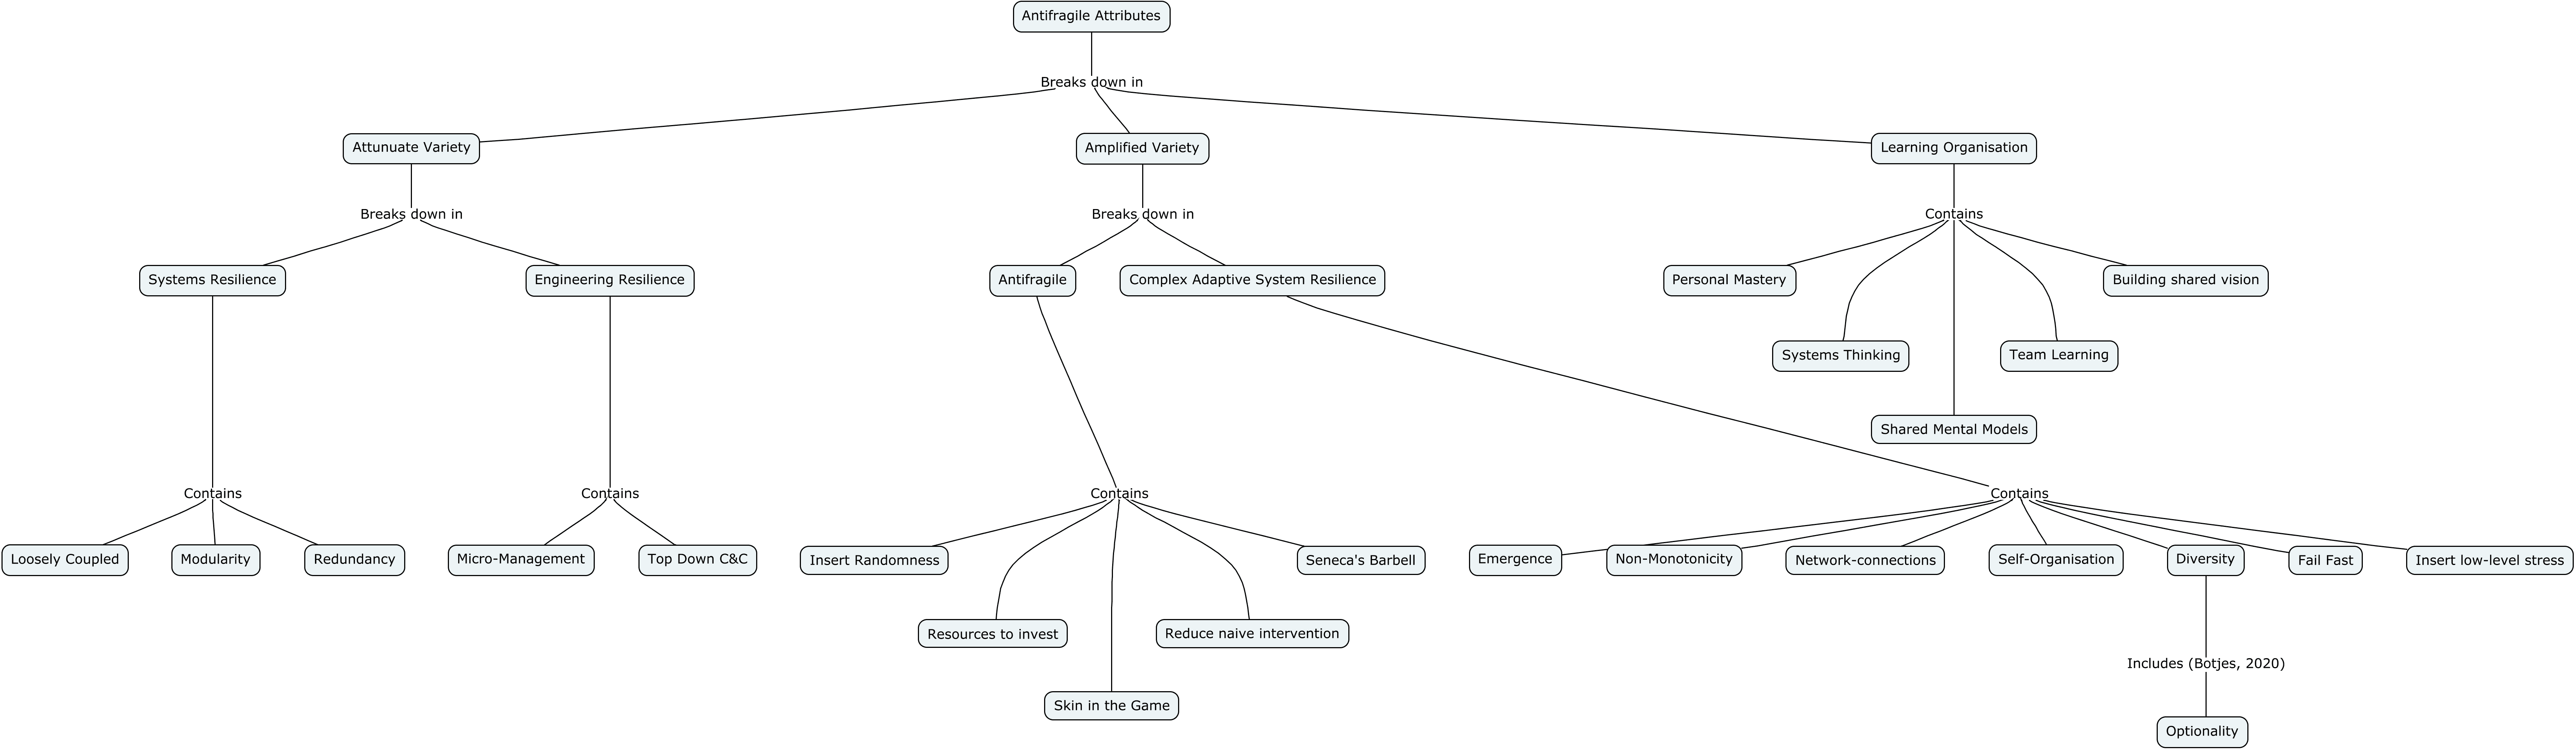
\includegraphics[width=0.9\linewidth]{images/cmapafattributes}
	\caption{Concept map of Antifragile Attributes}
	\label{fig:conceptmapafattributes}
\end{sidewaysfigure}
		%\appendix
\chapter{Antifragile literature June 2019--April 2022}
\label{app:literaturecatchup}
This appendix contains the newly found literature as a catch-up on the literature research of \textcite{Botjes2020}.

\begin{longtable}{p{.4\textwidth}p{.4\textwidth}p{0.1\textwidth}}
	\toprule%
	\textbf{Title} & \textbf{Author} & \textbf{Year} \\
	\midrule%
	\endhead%
	\hline
	\endfoot%
	\caption[Literature search June 2019--March 2022 all sources]{Literature search June 2019--March 2022 all sources}
	\label{tab:literatureafter2020all}
	\endlastfoot%
		A Barbell Strategy-oriented Regulatory Framework and Compliance Management & Gallina, Barbara & 2020 \\
		A collaborative approach to resilient and antifragile business ecosystems & Ramezani, Javaneh and Camarinha-Matos, Luis M. & 2019 \\
		A Game Theoretic Approach for Quality Assurance in Software Systems Using Antifragility-Based Learning Hooks & Vimaladevi, M. and Zayaraz, G. & 2020 \\
		A Literature Review of Organizational Resilience & Ping, Li Peter and Jiazhe, Zhu & 2021 \\
		A Philosophy of Security Architecture Design & Koien, Geir M. & 2020 \\
		Agile architecture & Kruchten, Philippe & 2013 \\
		An Introduction to Residuality Theory: Software Design Heuristics for Complex Systems. & O'Reilly, Barry M. & 2020 \\
		Antifragility as a design criterion for modelling dynamic systems & de Bruijn, Harald and Groessler, Andreas and Videira, Nuno & 2020 \\
		Approaches for resilience and antifragility in collaborative business ecosystems & Ramezani, Javaneh and Camarinha-Matos, Luis M. & 2020 \\
		Architecture Principles for Resilience & Furrer, Frank J & 2019 \\
		Beyond Resilience in Sociotechnical Systems & Simonette, Marcel and Magalhaes, Mario and Bertassi, Eduardo and Spina, Edison & 2019 \\
		Black-Swan Type Catastrophes and Antifragility/Supra-resilience of Urban Socio-Technical Infrastructures & Timashev, S. A. & 2020 \\
		Conceptualizing resilience in engineering systems: An analysis of the literature & Wied, Morten and Oehmen, Josef and Welo, Torgeir & 2020 \\
		Cybersecurity in the Internet of Things in Industrial Management & Raimundo, Ricardo Jorge and Rosario, Alberico Travassos & 2022 \\
		Ecosystem antifragility: beyond integrity and resilience & Equihua, Miguel and Espinosa Aldama, Mariana and Gershenson, Carlos and Lopez-Corona, Oliver and Munguia, Mariana and Perez-Maqueo, Octavio and Ramirez-Carrillo, Elvia & 2020 \\
		Emerging risk management in industry 4.0: an approach to improve organizational and human performance in the complex systems & Brocal, Francisco and Gonzalez, Cristina and Komljenovic, Dragan and Katina, Polinpapilinho F and Sebastian, Miguel A & 2019 \\
		Enterprise Architecture Resilience by Design: A Method and Case Study Demonstration & Aldea, Adina and Vaicekauskaite, Egle and Daneva, Maya and Piest, Jean Paul Sebastian & 2021 \\
		Enterprise Development Management through managed chaos & Kasianova, Nataliia and Tarasova, Elena and Kravchuk, Nataliia & 2019 \\
		Facing uncertainty: An entrepreneurial view of the future? & Bridge, Simon & 2021 \\
		Microservice Architecture & Nadareishvili, Irakli and Mitra, Ronnie and McLarty, Matt and Amundsen, Mike & 2019 \\
		No More Snake Oil: Architecting Agility through Antifragility & O'Reilly, Barry & 2019 \\
		On the meaning and operationalization of antifragility: Comment on the paper by Grossler & van Daalen, Els & 2020 \\
		Resilience, robustness, and antifragility: Towards an appreciation of distinct organizational responses to adversity & Munoz, Albert and Billsberry, Jon and Ambrosini, Veronique & 2022 \\
		Self-Improving Autonomic Systems for Antifragile Cyber Defence: Challenges and Opportunities & Chhetri, Mohan Baruwal and Uzunov, V, Anton and Vo, Quoc Bao and Nepal, Surya and Kowalczyk, Ryszard & 2019 \\
		The Business Transformation Framework and Enterprise Architecture Framework for Managers in Business Innovation The role of legacy processes in automated business environments & Trad, Antoine and IBISTM, France and Kalpic, Damir & 2017 \\
		The Machine in the Ghost: Autonomy, Hyperconnectivity, and Residual Causality & O'Reilly, Barry M. & 2021 \\
		The Philosophy of Residuality Theory & O'Reilly, Barry M. & 2021 \\
		The Tao way to anti-fragile software architectures: the case of mobile applications & Grassi, Vincenzo and Mirandola, Raffaela & 2021 \\
		Toward a commonly shared public policy perspective for analyzing risk coping strategies & Li, Yanwei and Taeihagh, Araz and de Jong, Martin and Klinke, Andreas & 2021 \\
		Tutorial on systems with antifragility to downtime & Hole, Kjell Jorgen & 2022 \\
		We need more Anti-Fragility! & Dirzus, Dagmar & 2020 \\
	\bottomrule%
\end{longtable}

%		\chapter{Interview Participants}
\label{app:interviewparticipants}

\begin{table}[!h]
	\begin{center}
		\begin{tabular}{@{}ccccc@{}}
			\toprule
			\textbf{Who} & \textbf{Role} & \textbf{From} \\ \midrule
			Christiaan Konstapel & Lead Enterprise Architect & Mileway \\
			Y    & 2    & tbd \\
			Y    & 2    & tbd \\ \bottomrule
		\end{tabular}
		\caption{Interview Participants}
		\label{tab:interviewparticipants}
	\end{center}
\end{table}
%		\chapter{Delphi Group Participants}
\label{app:delphigroupparticipants}

\begin{table}[!h]
	\begin{center}
		\begin{tabular}{@{}ccccc@{}}
			\toprule
			\textbf{Who} & \textbf{Role} & \textbf{From} \\ \midrule
			Jan Ploeg & Enterprise Architect & Centric Netherlands B.V. (ISV) \\
			Y    & 2    & Other ISV \\
			Y    & 2    & Municipality \\
			Y    & 2    & VNG-Realisatie \\
			Y    & 2    & Logius \\
			Z    & 0    & Academic \\ \bottomrule
		\end{tabular}
		\caption{Delphi Group Participants}
		\label{tab:delphigroupparticipants}
	\end{center}
\end{table}
		%\chapter{Literature Selection}
\label{app:literature_selection}


		%\appendix
\chapter{Interview summaries}
\label{app:interviewsummaries}
This appendix contains summaries per interview. This appendix gives the reader of this thesis more details on the answers given by the interviewees. These summaries are created from the recorded interviews and transcriptions belonging to these recordings.

\section{Interview central government}
\label{sec:interviewcentralgovernment}
\subsubsection{Question 1 / Enterprise Architecture}
\gls{ea} is not used and we are not \gls{agile}. \gls{ea} is too difficult for the public administrators. In addition, we are also responsible for other sectors. There is not one architecture. We have multiple reference architectures. What we have to do in the public sector depends on the political decision making within the period of governing (four years until new elections). \gls{ea} is at the end of the chain of administrative decision-making.
\subsubsection{Question 2 / Agility of the public sector}
It is hard to be \gls{agile} within the \gls{ps}. Everything needs to be predefined and planned. \Gls{agile} working is very difficult within the government. The end goal is not very clear with \gls{agile} working. It is unclear how the public money is spent on precisely what. 
\subsubsection{Question 3 / Dealing with uncertainty and unexpected events}
The \gls{ps} cannot deal with \gls{uncertainty}. Everything must be predefined and planned. There must be accountability for how public money is spent. All missteps are magnified. There is a quick result in crises, but with possible consequences later on because of \gls{bit} audits or  \glspl{parliamentaryinquiry}.
\subsubsection{Question 5 / The risk appetite of the public sector}
There is no risk appetite. Everything must be known and explainable in advance. If it is found that the procedures are not used, it can result in political consequences later on. Afterwards, positive lessons learned are not used to make adjustments within the public sector. Experimentation is (almost) not possible.
(note: blaming culture)
\subsubsection{Question 6 / The use of diversity and optionality in the public sector}
It would be nice to work with optionality and smaller units within the \gls{ps} and \gls{ea} to make it easier to adapt. Think about in \gls{ea} disposable microservices. Nevertheless, it remains that ea is not important. It is at the end of the chain and is not used in administrative decision-making. Enterprise architecture is confronted with decision-making.
\subsubsection{Closing statements}
\Gls{antifragile} is not directly applicable for the central government, but it can have a lot of benefits for suppliers in the \gls{ps}. Do not advertise it but exploit it to become better. In the case of an \acrfull{isv} think about many disposable microservices so it will be easier to deal with the \gls{ps}.
\section{Interview local government}
\label{sec:interviewlocalgovernment}
\subsubsection{Question 1 / Enterprise Architecture}
There is somewhat of an \gls{ea}, but we are not using it that broadly. As an organisation, we do not have a real \gls{ea}. Our organisation is best compared to that of a consultancy firm. Our core task is lobbying advocacy. We guide the things we do, and then again, it concerns the things we do for municipalities or on behalf of municipalities. We have a multi-year vision. We use guiding principles for the things we do.
Nevertheless, there are processes in the making for portfolio management. What do we do, what don't we do, and how do they relate to each other. There is not one responsibility on the \gls{ea}. It is a stepped responsibility that lies with committees and the services board. When it comes to IT, the responsibility lies with the Directory of Information Society. \gls{ea} is used for assay the request for subsidy. When there is a request for a subsidy that is not in line with the goals, it is not requested by the (European) government.
The case of how \gls{ea} contributes to the agility of the public sector is complicated. The public administrators are not architects and vice versa. \gls{ea} is hard to understand. \gls{ea} does not provide answers for the problems of today. Ultimately \gls{ea} should deliver this so the change can start tomorrow. It is essential to clarify the problems that public administrators are having. Both the facts as well the underlying causes. \gls{ea} should clarify the differences. Make it clear where we need to go and map out a path to get there, based on little steps that ultimately lead to the goal. Moreover, in the language public administrators understand. The architect must use the language of the stakeholders to make \gls{ea} successful (note: success factor).
\subsubsection{Question 2 / Agility of the public sector}
The \gls{ps} is more about risk aversion. Legality is about holding on to what is known. So, it is exactly known what the municipalities do, and we know precisely what the Land Registry does. All the subsystems of the \gls{ps} have a defined assignment. Moreover, it would be best if it stayed between the lines. Think, for example, about purpose limitation. Purpose Limitation will hold it back when \gls{ps} wants to be agile. The \gls{ps} cannot experiment that easily with rules like these. It will put experimentation at the edge.
The operating model of the \gls{ps} does not offer the freedom to do so that easily. The \gls{ps} can not experiment, discover and then say this was a nice experiment; let us go further. It is impossible to take decisions on the whole, such as within the social domain. If you have the right to confiscate a car, you cannot decide that there need to be a taxi to drive kids to school. It is a responsibility of a different part of the \gls{ps}. This all has to do with \gls{houseofthorbecke}\footnote{\url{https://www.denederlandsegrondwet.nl/id/vieqcpdzf0gw/bestuurlijke_indeling}} together with the current legislation and regulations. It does not mean that the \gls{ps} does not want to be more agile. It is not about separate parts of the government anymore. There is more and more collaboration based on federation. The \gls{ps} wants to be more agile. It is often a subject of conversation. Nevertheless, it gets stuck in the administrative decision-making processes.
\subsubsection{Question 3 / Dealing with uncertainty}
The reflex on \gls{uncertainty} of the \gls{ps} is that the \gls{ps} gets very insecure from \gls{uncertainty}. So the \gls{ps} does not know how to deal with \gls{uncertainty}. The common reflex is to push the uncertainty back to robust/resilient, so it is under control again. Robust \& resilient is back to its previous state but then sturdier, more robust (note: Risk avoidance). However, the \gls{ps} claims that they can deal with it. See, for example, the energy transition. The \gls{ps} defined the framework for this transition. It can contribute to the economy with many new jobs and a new knowledge model. We did see that also in the past with road and waterway engineering. Nevertheless, then they forget about the mechanisms needed to accomplish it. So the \gls{ps} does want to deal with \gls{uncertainty}, but the \gls{ps} is not creating the right conditions or the freedom of acting to be able to do so.
The available \gls{ea}'s within the \gls{ps} do not help either. It does not contribute to accept \gls{uncertainty}. At the most, our new vision on Information, Common Ground\footnote{\url{https://commonground.nl/}}, is contributing to this. An important principle in that vision is the ''community'' principle that could help with this \gls{uncertainty} (note: shared mental models). This principle states that municipalities, chain partners, market parties and the \acrshort{vngr} work together as a community in realisation. It is the certainty that it is uncertain. There are always new issues, and organising collaboration will help us to better deal with this \gls{uncertainty}, especially in the \gls{ps}.
\subsubsection{Question 4 / Dealing with unexpected events}
We, fortunately, live in a country where the \gls{ps} is staffed with good people who understand what citizens need or what is needed in a disaster area. So help is available pretty quickly. For example the fires at Moerdijk\footnote{\url{https://nl.wikipedia.org/wiki/Brand_Moerdijk_5_januari_2011}}, near Rotterdam. Or the plane crash of Turkish Airlines\footnote{\url{https://en.wikipedia.org/wiki/Turkish_Airlines_Flight_1951}} at Schiphol. Before we knew it, the fires were already distinguished. However, the \gls{ps} is not able to ascertain if it is an incident or a structural problem. If the problem takes too long, we see the reflex to control it again, so we fall back to our past habits. Adopting newly learned patterns is hard with the current legislation and regulations. Maybe we must be in a continuous crisis, so we have the freedom to do what we have to do. It is easier to be more agile in a crisis. With the local governments, there is only one who can decide what to do in a crisis, and this is the mayor as part of the triangle\footnote{\url{https://nl.wikipedia.org/wiki/Driehoek_(overheid)}}. 
It seems that the local governments have two organisation \& operational models. A model for running the municipality in a normal state and one in a state of crisis. (note: Seneca's Barbell?)
\subsubsection{Question 5 / The risk appetite of the public sector}
Drive and urge for innovation and change, which could perhaps be another interpretation of the word risk. People in the \gls{ps} want to find out if it can be done differently, but it is very dependent on the person. So actually, that depends on people in the \gls{ps}. Not on the \gls{ps} as a whole, based on intrinsic motivation to make things better for citizens and entrepreneurs. We have even set up our organisation in such a way that we can support this. Nowadays we have a department for research and innovation. But after something new is thought of it will go to the department to create it and finally to to a department to maintain it. Sometimes we are limited because it influences the standing legislation and regulations.
\subsubsection{Question 6 / The use of diversity and optionality in the public sector}
The \gls{ps} is not supporting diversity and optionality, but on the other hand the \gls{ps} is based on the absolute premise that all organisations are autonomous. (note: with a clear goal per organisation so no options). The implementation of the policies is extremely diverse. For example, there are various approaches known for people who are unemployed. One municipality forces people to perform work before they receive benefits, while another municipality supports them to be financially healthy again. Both achieve the obligation to provide care to a citizen so that the citizen has an income again. Diversity and optionality are less important. The local authorities simply have to implement the policies. It is all set down in the law and regulations. There is quite a diversity in how municipalities organize things. One municipality collects the household waste itself, while another has outsourced it. In both cases, the collection of household waste is arranged. Nobody prescribes how you arrange it, as long as it is arranged. You see the same thing within IT. However, you see here that for transitions and transformations an \gls{ea} is enormously needed to support the new world.
\subsubsection{Closing statements}
The government will not disappear, but that trust in the government will. Some government organizations or parts of them can undoubtedly disappear. (note: does not fit with the questions but find it an important statement).
The \gls{ps} needs a cross-sector \gls{ea}. It's no longer just about your organization. You have to work together more and more. The \gls{ea} can then be further tailored to your own organization.
\section{Interview Independent Software Vendor}
\label{sec:interviewisv}
\subsubsection{Question 1 / Enterprise Architecture}
Enterprise Architecture is developed to bring the business units together under one single architecture firstly. A common architecture brings synergy. It is reusing common components. Develop common language (note: Learning Organisation attribute shared mental model). It will bring us efficiency. Starting with architecture as a steering mechanism (note: engineering \gls{resiliency} attribute Command \& Control) and currently focusing on the internal organisation, the enterprise (note: mostly the first school of thought of \gls{ea} \parencite{Lapalme2012}). It is emerging that the current architecture is used as a communication mechanism to the external context (note: first steps into the second school of thought of \gls{ea} \parencite{Lapalme2012}). Our \gls{ea} is supporting us with the transformation towards a \acrfull{saas} provider. The \gls{ea} is used more and more used as a mechanism for explaining. The focus of the \gls{ea} is at this moment 80\% on the internal organisation and 20\% on the external context (note: not yet the third school of thought of \gls{ea}).
\gls{ea} is the responsibility of the \acrfull{coo} but the group of executive management is accountable. This group contains the \acrfull{ceo}, the \acrshort{coo} and the \acrfull{cco}. (note: with placing the responsibility on \gls{ea} with the \acrshort{coo} the primary purpose of \gls{ea} will be efficiency). The interviewee (\acrshort{ceo}) does not worry about this because in the end everything ends up with the \gls{ea}. \gls{ea} must be part of the executives. \gls{ea} is essential for business operations.
Our \gls{ea} supports us to be agile. Our crown jewels (our applications) are a stable core around which we can be flexible and agile to follow external contexts such as new laws and legislation. Think about the \acrfull{api} layer (note: systems \gls{resiliency} attribute Loosely Coupled) that is being built that makes it easier to respond to these changes. Eventually, our \gls{ea} must enable us to change to support our customers with their social tasks. We are not there yet. The transformation towards \acrfull{saas} alone takes us multiple years. This is, at this moment, not a problem yet.
The \gls{ps} is even moving slower, and there is not that much competition, but it is changing rapidly. The pace of change is increasing. It can be said that sometimes there is already a permanent state of change. Take the replanning of the municipalities and shifting tasks from the centralised government to the local government. The role of technology gets even more critical, the civilians are getting more empowered, and the participation rate in society increases. The influence of the external contexts does have more and more influence. Only the digital transformation itself is a stressor on the \gls{ps}. It already was there, but we see an increase. At this moment, the policymakers (politics) limit the speed of change.
These are not isolated incidents. An example is the ''Digitaal Stelsel Omgevingswet'', which is again being postponed. This is not sustainable in the near future. If this does not change, the \gls{ps} will get stuck.
\subsubsection{Question 2 / Agility of the public sector}
The current operational model of the \gls{ps} is old and moves slowly because of the regulations, legislation and qualified-majority decision-making. However, when there is a crisis, everything is possible. But only under extraordinary conditions. The \acrshort{ps} should be in a continuous crisis (note: looks like the \gls{antifragile} attribute of insert randomness). After a crisis, lessons learned are not used to improve the public sector (note: attribute part of the learning organisation). There is no feedback loop. The system is not supporting this. Changes to the current systems are slow, complex and large. Because of this, there are not that many suppliers on some solutions. For several solutions, there is only a choice between two (note: the \acrshort{cas} attribute diversity and optionality is not available.). In the worst case, there is only one solution, like with the taxes administration of the Ministery of Finance. The architectures in the \acrshort{ps} cannot support it because it misses alignment with business language. It misses stakeholder specific views in the language of the stakeholders. A good example is the \acrfull{idea}\footnote{\url{https://www.ictu.nl/projecten/idea-beeldtaal-maakt-it-infrastructuur-begrijpelijk}} method of the government. However, they stopped using it. 
Most IT management in the Public Sector is not IT Savvy. It would be better to have IT Savvy Management experienced with policymaking. The IT Systems contain much technical debt. To the extent that the systems with new functionality often use encapsulation. Adjusting IT Systems take much time with many risks. The impact of a new coalition agreement is high. With a coalition agreement, many high-impact system adjustments must be made. The policymakers expect changes to be executed in only a couple of days. In the past, public sector organisations were loosely coupled and were highly cohesive (clear goal). With all those policy changes, organisations even got strangled and cannot be adjusted that easily anymore, like with the taxes administration of the Ministery of Finance as an Example. The taxes administration was specialised in collecting taxes (note: Systems Resilience attribute Loosely Coupled (High Cohesion)). Policymakers also forced them to disbursement (note: Systems Resilience attribute antipattern with result tightly coupled with low cohesion). The same departments, processes and systems were used.
\subsubsection{Question 3 / Dealing with uncertainty}
You cannot define uncertainty on the public sector as a whole. The average size of municipalities is growing because of the reordering of Municipalities. Municipalities that are too small are merged (note: decrease of modularity, self-organisation and diversity). The scaling of municipalities is not always in the best interest of the civilians. It does not always improve the services to the residents of the municipalities. There are cases where a civilian needs to cycle 10km for a passport while it was less in the old situation. The services given are more business-like without a personal touch. If you look at the \gls{ps} for the last 200 years, the \gls{ps} is capable of adjusting when it needs to be adjusted (note: resilient/robust). The \gls{ps} can deal with uncertainty. However, if the way the \gls{ps} deals with uncertainty is the most efficient way is the question. The social cohesion that the civil servants of the \gls{ps} have is enormous. The \gls{ps} can handle uncertainty. The will is intrinsic available. If they get an assignment, they are going for it. If it must be done within four years (the duration of a coalition agreement), they will go for it. Even if the change is too big or complex and the planning is not realistic.
An example of the effect is that of the childcare benefits scandal\footnote{\url{https://en.wikipedia.org/wiki/Dutch_childcare_benefits_scandal}}. Decentralisation of governmental tasks was the cause of this. Because of the absence of \gls{ea} and the usage of \gls{ea} within the \acrshort{ps} domains, such as social domain, taxes, finance, a.o., these examples are not an incident. \gls{ea} can prevent these causes and effects. The fact that the \gls{ps} did not organise \gls{ea} is a cause of the incidents. The actual absence is an \gls{ea} process that guides the governments. This behaviour is especially shown with the local governments. They are continuously reinventing the wheel (note: No overarching Command \& Control). The \gls{ps} has to go back to the drawing board for every change to develop a new approach.
\subsubsection{Question 4 / Dealing with unexpected events}
The \gls{ps} is handling unexpected events better than uncertainty. The \gls{ps} handles unexpected events better than the political decisions made by coalition agreements. In a crisis situation, the \gls{ps} is capable of working very effectively. Should the \gls{ps} be in an ongoing crisis? No. The \gls{ps} is in need for \gls{antifragile} solutions. Better is to continuously add a small amount of stress to the \gls{ps} system (note: antifragile attribute insert randomness). This is in contrast to sitting back and watching until something happens. It seems that the rules do not apply anymore with an unexpected event. The \gls{ps} has many talents to deal with these situations, but they all seem too busy with their careers, salaries, what should go to which ministry, and others. This is the thing that needs to be solved. Strange because most of the time, the employees in the \gls{ps} enjoy working in a crisis. It makes them feel proud that they accomplished something. There were initiatives to use \gls{ea}, and it proved to be supporting the changes. Overarching examples are, for example, the consolidation of 66 datacenters to two private and two public datacenters (note: diversity and optionality), the common desktop standard (project ''goud'') (note: part of the stable part of Seneca's barbell strategy). Re-usability, an ICT dashboard, and many more initiatives were worked on. Later on, these initiatives fell apart, and the ministries picked it up again in their silo. It all was carried by a select group of people in the \gls{ps}. It all fell apart when some of them left the \gls{ps}. If it does not have assignments from the government members, it is dependent on the willingness to cooperate. The dominance of the separate ministries take the overhand, and people fall back in the old habits. To sustain the use of \gls{ea} it should not depend on a selective group of people but on the \gls{ps} itself (note: success factor). The mutual differences are gone when there is a common enemy (an unexpected event). At that moment, the solution will overarch the \gls{ps}. Changes following the process have less effect than changes initiated by chaos. The feedback from unexpected events is not fed into the system so that it can be changed (note: learning organisation not in place).
\subsubsection{Question 5 / The risk appetite of the public sector}
For the risk appetite of the \gls{ps}, the government members have an essential role. At this moment, there is no culture of risk-taking. Even worse, taking risks can have serious consequences. Think about, for example, commission ''Elias'' \footnote{\url{https://nl.wikipedia.org/wiki/Parlementair_onderzoek_ICT-projecten_bij_de_overheid}}. Because of this commission, a new department, \gls{bit}, was started as part of the Ministry of Home Affairs with the assignment to assess all the IT Projects within the centralised government (note: Engineering Resilience attribute Command \& Control). Because of this, people are not willing to take risks anymore (note: insert randomness, tinkering, naive interventions, monotonicity, fail-fast, and others). Some are busy shielding their bosses and managers for possible errors (note: \gls{antifragile} attribute: (no) skin in the game). At this moment, the \gls{ps} is showing risk avoidance behaviour. The base attitude of the \gls{ps} is that it does not have a risk appetite. Partly because of public opinion. It is all about the use of public funds. Before you know it, there will be negative attention in the media. \gls{ea} is mostly used in a prescriptive way (note: Engineering Resilience attribute Command \& Control). The \gls{ps} is not foster a safe environment for experimentation. Even when a good solution is implemented in a time of crisis (unexpected events), punishment will happen afterwards because it did not comply in the way it usually should. The \gls{ps} public sector created an environment in which the \gls{ps} is a fragile ''glass house'' together with a culture of blaming. So the risk appetite is getting less and less.
\subsubsection{Question 6 / The use of diversity and optionality in the public sector}
Optionality does not have a chance in the \gls{ps} because of european tender obligations. The european tenders are mostly about risk reduction. The european tenders contain many legal conditions. But not only legal conditions but also a lot of technical conditions. Everything is defined in a way that you have no options anymore. The conditions are even so that you cannot choose, for example, multiple suppliers so you will have options during the contract periods. The private sector has this already for a long time. There are private companies who have multiple suppliers for a domain. If one supplier is not delivering the quality anymore another supplier is taking over. European tenders did not help us to become more flexible, resilient, and agile. But there are changes. It would be nice to see if the \acrfull{vngr} will be thinking of a broker construction with multiple suppliers. By using this strategy the local governments can choose a supplier by only using bids. It is easier to switch and having options. Another thing that can help optionality is defining right \acrfull{kpi}'s. If you define a KPI in such a way that the performance of a supplier is measured by the ease of transitioning to another supplier it will get easier to switch suppliers. This has a positive influence on executing optionality. But this way of working is not sustained in, for example, the \gls{ea}.
\subsubsection{Closing statements}
The digital transformation must be important to everyone and not only to a minister of digital affairs. How do you make sure that business management of the \gls{ps} find it normal to discuss IT, budget, personnel, organisational configuration, and others? If they start thinking like this, they will find out what \gls{ea} can do for them. If we know how to close this gap, digital transformation will get the proper attention. We also have to thank ourselves for this because of the use of non-business language.
\section{Interview consultancy firm/service provider}
\label{sec:interviewconsultancyfirm}
\subsubsection{Question 1 / Enterprise Architecture}
We have, to an extent, an \gls{ea} with the necessary elements for the products and services we develop ourselves. We do not have a dedicated enterprise architect. Other types of architects maintain the current \gls{ea}. The \acrshort{cto} is accountable for the \gls{ea}. In the end, everything rolls up to the \acrshort{ceo}. 

Our \gls{ea} is, at this moment, mostly about our products and services and addresses our primary concerns. The concerns are the connections between data, how they should communicate, and the impact on our products and services. With the \gls{ea}, we can determine our solution gaps and steer towards procurement of applications and integrations. The integrations are with the sales, finance, HR, and delivery capabilities. We still have two separate worlds in our organisation. These two worlds are the supporting and delivery capabilities of our organisation. Bringing these two worlds together will be on the roadmap for next year so we can work with an integrated \gls{ea}. Both worlds come together when we think about our customers. We will realise that when we develop features for our platform, we can connect to the propositions that we offer to our customers. The lack of an \gls{ea} slows us down from achieving this. We do not have a business architecture, but we advise our customers on business architecture. We have to close this gap. 

With the current \gls{ea} we can make adjustments to our products and services very fast and flexible. Our \gls{ea} supports it because it contains the architecture of our products and services and our infrastructure down to the data models that we use for our customers. However, we do not have control over our supporting applications, such as Salesforce. Our products and services are \gls{robust} \& \gls{resilient} and support us to be \gls{agile}. Sometimes we disconnect a server to see what happens (note: insert randomness / SRE / Chaos Engineering). We continuously improve ourselves to get better (note: learning organisation).
\subsubsection{Question 2 / Agility of the public sector}
There is a low degree of agility in the \gls{ps}. This low \gls{agility} is possible because of the lack of IT knowledge and skills in politics and policymakers. If we look at the electoral lists of the central and local elections, we can state that there is a shortage of knowledge, skills and fundamental IT knowledge. There are exceptions, but not that much.

If we compare this to, for example, the Estonian model, we see a world of difference. We are not there (yet). We have to invest more in this. If we think of the \gls{ps} as an aggregate and you go lower in the aggregation, you already see that it is going better. We see that the \gls{ps} has been taking significant steps in the last ten years. Administrative governmental agencies have more responsibilities to operationalise, develop and maintain systems. We have been able to leave a mark in the \acrshort{ps} on the technical quality of systems. It is a good development that the \acrshort{bit} exists. The operating model of the \gls{ps} is extending. Compared to the private sector, the government is at a good average. Maybe this is already a good position for the government. We will see more and more connections and integrations with specific ministries and administrative agencies. The digital transformation is progressing. More and more is shared online and is easy to access. We see this as a positive effect. We can help the \gls{ps} further because of this by bringing in best practices. How should we unlock our data, what can we do with this data, and what is the effect on IT and Governance. \gls{ea} can support us in this.
\subsubsection{Question 3 / Dealing with uncertainty}
We see the desire for robustness \& resilience. The \gls{ps} tries to push it back to how it was. As an example, the regulations on electric steps. It is a new development, and it falls outside the scope of current regulations. It is not a scooter or a bicycle, and it does not fit in any other regulations. The reaction of the policymakers is to rule it out. It is not allowed until there is an agreement on new regulations. The Dutch model is to push it back to how it was. The electric steps are allowed if there is an agreement on how to allow them. We see the same behaviour with the  IT capability. Policymaking takes time. It slows down new developments. The choices are made based on robustness, certainty and clarity. The behaviour has everything to do with the risk aversion of the \gls{ps}.

The basic attitude of the \gls{ps} is to avoid mistakes. When a choice has a risk, they do not decide until everything is clear. There is an implicit postponement in this behaviour. The risk of this behaviour is that the \gls{ps} is missing great opportunities. The founding of \acrshort{bit} is an excellent thing to have some certainty, but it is concerning that the whole \gls{ps} is moving towards control and risk mitigation. It removes agility from the system while the government plays a facilitating role in our society. All risks should be avoided, and everything needs to be traceable, making no mistakes. By this approach, the \gls{ps} is probably missing out on options that can make a difference, and it inhibits realising potentials. The \gls{ps} is using \gls{ea} as a way to attenuate. 
\subsubsection{Question 4 / Dealing with unexpected events}
If something happens, there is the will to act by setting up something new, reworking systems, and other things. Nevertheless, there still is a considerable delay after the unexpected event happened. After achieving the goal is directly followed up by attenuation. The \gls{ps} does not want to make mistakes, so the \gls{ps} will do as minimal as possible to achieve the goal because of risk mitigation.

If something happens, the \gls{ps} deals with that. However, because of the aversion to risks, the \gls{ps} is not getting the most out of it. If the \gls{ps} exploits the situation, instead of familiar ways, with more radical approaches, the result will be a significant progression, even when there is uncertainty. It is another way of doing so with the risk that something will go wrong. If it goes wrong, there is a risk that the press will magnify it because it is about spending public money. Unfortunately, successes do not get attention.
\subsubsection{Question 5 / The risk appetite of the public sector}
We want to play a role in this world by being more innovative. We allow some governmental bodies to go a little further in experimentation and development, but this is mainly on a project-by-project basis. For these projects, we accepted that it would cost us public money and that making mistakes is allowed. However, generically, the trajectories we see do not have a risk appetite and are even risk-averse. Most of the time, this is good for a reliable government. Use, for risk-taking cases, specific demarcated parts of the \gls{ps}.
\subsubsection{Question 6 / The use of diversity and optionality in the public sector}
We see an improvement on this topic over the past years in the \gls{ps}. We see a growth in knowledge, from an IT perspective, in multiple areas in the \gls{ps}. E.g. architecture, implementation, development, code quality and other qualitative aspects of IT. We see, at this moment, this contribution mainly from the central government and not so much from the local governments. We think that this improvement will continue. We do hope that this improvement will reach the electoral lists. If we look at the systems, we do not see any uniformity. We do see differences in designs and the ways of looking at things.
		\chapter{Interview findings}
\label{app:interviewfindings}
This appendix describes the interview findings in more details. This appendix can be used by the reader of the thesis with more detailed information.
\begin{table}[htbp]
	\centering
	\begin{tabular}{lllll}
		\toprule
		\textbf{Code} & \multicolumn{1}{l}{\textbf{Count}} & \multicolumn{1}{l}{\textbf{\% Codes}} & \multicolumn{1}{l}{\textbf{Cases}} & \multicolumn{1}{l}{\textbf{\% Cases}} \\
		\midrule
		Top Down CC &  18    & 3,10\% & 4     & 100,00\% \\
		No Top Down CC & 2     & 0,30\% & 1     & 25,00\% \\
		Micro-Management & 17    & 2,90\% & 4     & 100,00\% \\
		No Micro-Management & 2     & 0,30\% & 1     & 25,00\% \\
		\bottomrule
	\end{tabular}%
	\caption{Interview results Engineering Resilience}
	\label{tab:interviewresultsengineeringresilience}%
\end{table}%

\begin{table}[htbp]
	\centering
	\begin{tabular}{lllll}
		\toprule
		\textbf{Code} & \textbf{Count} & \textbf{\% Codes} &\textbf{Cases} & \textbf{\% Cases} \\
		\midrule
		Redundancy & 3     & 0,50\% & 3     & 75,00\% \\
		No Redundancy & 1     & 0,20\% & 1     & 25,00\% \\
		Modularity & 5     & 0,90\% & 3     & 75,00\% \\
		No Modularity & 3     & 0,50\% & 1     & 25,00\% \\
		Loosely Coupled & 5     & 0,90\% & 3     & 75,00\% \\
		Not Loosely Coupled &       &       &       &  \\
		\bottomrule
	\end{tabular}%
		\caption{Interview results Systems Resilience}%
	\label{tab:interviewresults Systems Resilience}%
\end{table}%

\begin{table}[htbp]
	\centering
	\begin{tabular}{lllll}
		\toprule
		\textbf{Code} & \textbf{Count} & \textbf{\% Codes} &\textbf{Cases} & \textbf{\% Cases} \\
		\midrule
		Diversity & 15    & 2,60\% & 3     & 75,00\% \\
		No Diversity & 9     & 1,60\% & 2     & 50,00\% \\
		Optionality & 12    & 2,10\% & 3     & 75,00\% \\
		No Optionality & 13    & 2,30\% & 4     & 100,00\% \\
		Mono-Monotonicity & 3     & 0,50\% & 2     & 50,00\% \\
		No Mono-Monotonicity & 13    & 2,30\% & 4     & 100,00\% \\
		Emergence & 3     & 0,50\% & 3     & 75,00\% \\
		No Emergence & 3     & 0,50\% & 1     & 25,00\% \\
		Self-Organisation & 3     & 0,50\% & 2     & 50,00\% \\
		No Self-Organisation & 3     & 0,50\% & 3     & 75,00\% \\
		Insert Low Level Stress & 19    & 3,30\% & 3     & 75,00\% \\
		No Insert Low Level Stress & 6     & 1,00\% & 3     & 75,00\% \\
		Network-Connections & 2     & 0,30\% & 1     & 25,00\% \\
		No Network-Connections &       &       &       &  \\
		Fail Fast & 6     & 1,00\% & 3     & 75,00\% \\
		No Fail Fast & 12    & 2,10\% & 3     & 75,00\% \\
		\bottomrule
	\end{tabular}%
	\caption{Interview results Complex Adaptive Systems Resilience}
	\label{tab:interviewresultscasresilience}%
\end{table}%

\begin{table}[htbp]
	\centering
	\begin{tabular}{lllll}
		\toprule
		\textbf{Code} & \textbf{Count} & \textbf{\% Codes} & \textbf{Cases} & \textbf{\% Cases} \\
		\midrule
		Resources to Invest & 7     & 1,20\% & 3     & 75,00\% \\
		No Resources to Invest & 7     & 1,20\% & 3     & 75,00\% \\
		Seneca's Barbell & 9     & 1,60\% & 3     & 75,00\% \\
		No Seneca's Barbell & 6     & 1,00\% & 3     & 75,00\% \\
		Insert Randomness & 8     & 1,40\% & 3     & 75,00\% \\
		No Insert Randomness & 6     & 1,00\% & 3     & 75,00\% \\
		Reduce naive intervention & 6     & 1,00\% & 2     & 50,00\% \\
		Skin in the Game & 3     & 0,50\% & 2     & 50,00\% \\
		No skin in the game & 5     & 0,90\% & 2     & 50,00\% \\
		\bottomrule
	\end{tabular}%
	\caption{Interview results Antifragile}
	\label{tab:interviewresultsantifragile}%
\end{table}%

\begin{table}[htbp]
	\centering
	\begin{tabular}{lllll}
		\toprule
		\textbf{Code} & \textbf{Count} & \textbf{\% Codes} & \textbf{Cases} & \textbf{\% Cases} \\
		\midrule
		Personal Mastery & 5     & 0,90\% & 3     & 75,00\% \\
		No Personal Mastery & 1     & 0,20\% & 1     & 25,00\% \\
		Shared Mental Models & 23    & 4,00\% & 3     & 75,00\% \\
		No Shared Mental Models & 17    & 2,90\% & 3     & 75,00\% \\
		Building Shared Vision & 16    & 2,80\% & 3     & 75,00\% \\
		No Building Shared Vision & 13    & 2,30\% & 3     & 75,00\% \\
		Team Learning & 5     & 0,90\% & 3     & 75,00\% \\
		No Team Learning & 2     & 0,30\% & 2     & 50,00\% \\
		Systems Thinking & 3     & 0,50\% & 2     & 50,00\% \\
		No Systems Thinking & 1     & 0,20\% & 1     & 25,00\% \\
		\bottomrule
	\end{tabular}%
	\caption{Interview results Learning Organisation}%
	\label{tab:interviewresultslearningorganisation}%
\end{table}%

\begin{table}[htbp]
	\centering
	\begin{tabular}{lllll}
		\toprule
		\textbf{Code} & \textbf{Count} & \textbf{\% Codes} & \textbf{Cases} & \textbf{\% Cases} \\
		Enterprise IT Architecting & 5     & 0,90\% & 3     & 75,00\% \\
		Enterprise Integrating & 7     & 1,20\% & 2     & 50,00\% \\
		Enterprise Ecological Adaption & 5     & 0,90\% & 2     & 50,00\% \\
		\bottomrule
	\end{tabular}%
	\caption{Interview results Enterprise Architecture schools of thought}%
	\label{tab:interviewresultseaschools}%
\end{table}%


\begin{table}[htbp]
	\centering
	\begin{tabular}{lllll}
		\toprule
		\textbf{Code} \textbf{Description} & \textbf{Count} & \textbf{\% Codes} & \textbf{Cases} & \textbf{\% Cases} \\
		\midrule
		Adapt to business language & 18    & 3,10\% & 4     & 100,00\% \\
		No Safe Environment & 7     & 1,20\% & 2     & 50,00\% \\
		Blaming Culture & 12    & 2,10\% & 3     & 75,00\% \\
		Limited EA & 15    & 2,60\% & 4     & 100,00\% \\
		Agility & 14    & 2,40\% & 3     & 75,00\% \\
		No Agility & 18    & 3,10\% & 4     & 100,00\% \\
		Robust/Resilient & 23    & 4,00\% & 3     & 75,00\% \\
		Fragile &       &       &       &  \\
		Tekort aan IT kennis & 4     & 0,70\% & 2     & 50,00\% \\
		Benchmarked to Estonia/Sweden & 2     & 0,30\% & 2     & 50,00\% \\
		Development of knowledge & 2     & 0,30\% & 1     & 25,00\% \\
		Applying Best Practices & 3     & 0,50\% & 2     & 50,00\% \\
		Governance & 37    & 6,40\% & 4     & 100,00\% \\
		Conservative & 14    & 2,40\% & 3     & 75,00\% \\
		Social Responsibility & 14    & 2,40\% & 4     & 100,00\% \\
		Risk Avoidance & 32    & 5,50\% & 4     & 100,00\% \\
		Tinkering & 6     & 1,00\% & 3     & 75,00\% \\
		Stressor & 18    & 3,10\% & 2     & 50,00\% \\
		\bottomrule
	\end{tabular}%
	\caption{Interview results Findings}%
	\label{tab:interviewresultsfindings}%
\end{table}%



		%\appendix
\chapter{Data preparation for interview analysis}

\section{Step 1: merge similar labels}


\section{Step 2: Filter cases on threshold}



\subsection{Outcome of filter cases on threshold}

\begin{table}[H]
	\centering
	\begin{tabular}{lllll}
		\toprule
		\textbf{Code} & \textbf{Count} & \textbf{\% Codes} &\textbf{Cases} & \textbf{\% Cases} \\
		\midrule
		Engineering Resilience & 60    & 10,40\% & 4     & 100,00\% \\
		Top Down CC & 18    & 3,10\% & 4     & 100,00\% \\
		Micro-Management & 17    & 2,90\% & 4     & 100,00\% \\
		\bottomrule
	\end{tabular}%
	\caption{Results of filtering cases Engineering Resilience on threshold}%
	\label{tab:resultsfilteringengineeringresilience}%
\end{table}%

\begin{table}[H]
	\centering
	\begin{tabular}{lllll}
		\toprule
		\textbf{Code} & \textbf{Count} & \textbf{\% Codes} &\textbf{Cases} & \textbf{\% Cases} \\
		\midrule
		Redundancy & 3     & 0,50\% & 3     & 75,00\% \\
		Modularity & 5     & 0,90\% & 3     & 75,00\% \\
		Loosely Coupled & 5     & 0,90\% & 3     & 75,00\% \\
		\bottomrule
	\end{tabular}%
	\caption{Results of filtering cases Systems Resilience on threshold}%
	\label{tab:resultsfilteringsystemsresilience}%
\end{table}%

\begin{table}[htbp]
	\centering
	\begin{tabular}{lllll}
		\toprule
		\textbf{Code} & \textbf{Count} & \textbf{\% Codes} &\textbf{Cases} & \textbf{\% Cases} \\
		\midrule
		Complex Adaptive System Resilience & 14    & 2,40\% & 3     & 75,00\% \\
		No Complex Adaptive System Resilience & 18    & 3,10\% & 4     & 100,00\% \\
		Diversity & 15    & 2,60\% & 3     & 75,00\% \\
		Optionality & 12    & 2,10\% & 3     & 75,00\% \\
		No Optionality & 13    & 2,20\% & 4     & 100,00\% \\
		No Mono-Monotonicity & 13    & 2,20\% & 4     & 100,00\% \\
		Emergence & 3     & 0,50\% & 3     & 75,00\% \\
		No Self-Organisation & 3     & 0,50\% & 3     & 75,00\% \\
		Insert Low Level Stress & 19    & 3,30\% & 3     & 75,00\% \\
		No Insert Low Level Stress & 6     & 1,00\% & 3     & 75,00\% \\
		Fail Fast & 6     & 1,00\% & 3     & 75,00\% \\
		No Fail Fast & 12    & 2,10\% & 3     & 75,00\% \\
		\bottomrule
	\end{tabular}%
	\caption{Results of filtering cases Complex Adaptive Systems Resilience on threshold}%
	\label{tab:resultsfilteringcasresilience}%
\end{table}%

\begin{table}[htbp]
	\centering
	\begin{tabular}{lllll}
		\toprule
		\textbf{Code} & \textbf{Count} & \textbf{\% Codes} &\textbf{Cases} & \textbf{\% Cases} \\
		\midrule
		Resources to Invest & 7     & 1,20\% & 3     & 75,00\% \\
		No Resources to Invest & 11    & 1,90\% & 3     & 75,00\% \\
		Seneca's Barbell & 9     & 1,60\% & 3     & 75,00\% \\
		No Seneca's Barbell & 6     & 1,00\% & 3     & 75,00\% \\
		Insert Randomness & 8     & 1,40\% & 3     & 75,00\% \\
		No Insert Randonmness & 6     & 1,00\% & 3     & 75,00\% \\
		\bottomrule
	\end{tabular}%
	\caption{Results of filtering cases Antifragile on threshold}%
	\label{tab:resultsfilteringantifragile}%
\end{table}%

\begin{table}[htbp]
	\centering
	\begin{tabular}{lllll}
		\toprule
		\textbf{Code} & \textbf{Count} & \textbf{\% Codes} &\textbf{Cases} & \textbf{\% Cases} \\
		\midrule
		Learning Organisation & 8     & 1,40\% & 4     & 100,00\% \\
		Personal Mastery & 5     & 0,90\% & 3     & 75,00\% \\
		Shared Mental Models & 23    & 4,00\% & 3     & 75,00\% \\
		No Shared Mental Models & 17    & 2,90\% & 3     & 75,00\% \\
		Building Shared Vision & 16    & 2,80\% & 3     & 75,00\% \\
		No Building Shared Vision & 13    & 2,20\% & 3     & 75,00\% \\
		Team Learning & 5     & 0,90\% & 3     & 75,00\% \\
		\bottomrule
	\end{tabular}%
	\caption{Results of filtering cases Learning Organisation on threshold}%
	\label{tab:resultsfilteringlearningorganisation}%
\end{table}%

\begin{table}[htbp]
	\centering
	\begin{tabular}{lllll}
		\toprule
		\textbf{Code} & \textbf{Count} & \textbf{\% Codes} &\textbf{Cases} & \textbf{\% Cases} \\
		\midrule
		Adapt to business language & 18    & 3,10\% & 4     & 100,00\% \\
		No Safe Environment & 19    & 3,30\% & 3     & 75,00\% \\
		Social Responsibility & 14    & 2,40\% & 4     & 100,00\% \\
		Risk Avoidance & 46    & 8,00\% & 4     & 100,00\% \\
		\bottomrule
	\end{tabular}%
	\caption{Results of filtering cases other findings on threshold}%
	\label{tab:resultsfilteringotherfindings}%
\end{table}%

\begin{table}[htbp]
	\centering
	\begin{tabular}{lllll}
		\toprule
		\textbf{Code} & \textbf{Count} & \textbf{\% Codes} &\textbf{Cases} & \textbf{\% Cases} \\
		\midrule
		Enterprise IT Architecting	& 21	& 3,60\%	& 4	& 100,00\% \\%		
		\bottomrule
	\end{tabular}%
	\caption{Results of filtering cases Enterprise Architecture schools of thought on threshold}%
	\label{tab:resultsfilteringenterprisearchitecture}%
\end{table}%

\section{Step 3:}



\section{Step 4: Joining positives and negatives}

\begin{table}[htbp]
	\centering
	\begin{tabular}{p{.05\textwidth}p{.5\textwidth}p{.45\textwidth}}
		\toprule
		\textbf{Step} & \textbf{Description} & \textbf{Rationale} \\
		\midrule
		1     & Rationalize Positives and negatives by add/substract & Bringing the values back to the found success factors/attributes \\
		\bottomrule
	\end{tabular}%
	\caption{Data preparation 4 - Joining positives with negatives}
	\label{tab:prepjoinpositiveswithnegatives}%
\end{table}%


		\chapter{Validation findings}

\section{Experience of validation group participants}

\begin{table}[!h]
	\centering
	\begin{tabular}{p{.55\textwidth}ccc}
		\toprule
		\textbf{Question} & \textbf{Rating} & \textbf{Variability} & \textbf{Abstains} \\
		\midrule
		How many years of experience do you have in the field of enterprise architecture? & 9,8 & 8\% & 0 \\%
		How many years have you worked as an (enterprise) architect? & 10,6 & 12\% & 0 \\%
		How many years of experience do you have in the field of complexity sciences (like antifragile)? & 7,4 & 16\% & 0 \\%
		How many years of experience do you have with the public sector? & 12,2 & 17\% & 0 \\%
		How many years of experience do you have with working in publicly-held organisations? & 10 & 16\% & 0 \\%
		How many years of experience do you have with working in privately-held organisations? & 17,2 & 21\% & 0 \\%
		\bottomrule
	\end{tabular}%
	\caption{Experience of validation group participants}
	\label{tab:appexperiencevalidationgroup}%
\end{table}%
\newpage
\section{Validation of antifragile attributes}

\begin{table}[!h]
	\centering
	\begin{tabular}{p{.55\textwidth}ccc}
		\toprule
		\textbf{Attribute} & \textbf{Rating} & \textbf{Variability} & \textbf{Abstains} \\
		\midrule
		Optionality & 6,9 & 32\% & 0 \\%
		Mono-Monotonicity & 7 & 51\% & 0 \\%
		Self-Organisation & 8,2 & 23\% & 0 \\%
		Fail-Fast & 7,8 & 35\% & 0 \\%
		Resources to Invest & 6,7 & 36\% & 1 \\%
		Seneca's Barbell & 5,8 & 37\% & 1 \\%
		Safe working environment & 7,4 & 31\% & 0 \\%
		Naar buiten kijken, samenwerking zoeken & 6,2 & 55\% & 0 \\%
		Data Governance planes (tbv infrastructure-as-code / Software Defined Anything) & 4,4 & 56\% & 1 \\%
		\bottomrule
	\end{tabular}%
	\caption{Validation of antifragile attributes}
	\label{tab:appvalidationofantifragileattributes}%
\end{table}%
\newpage
\subsection{Optionality}
\begin{figure}[h!]
	\centering
	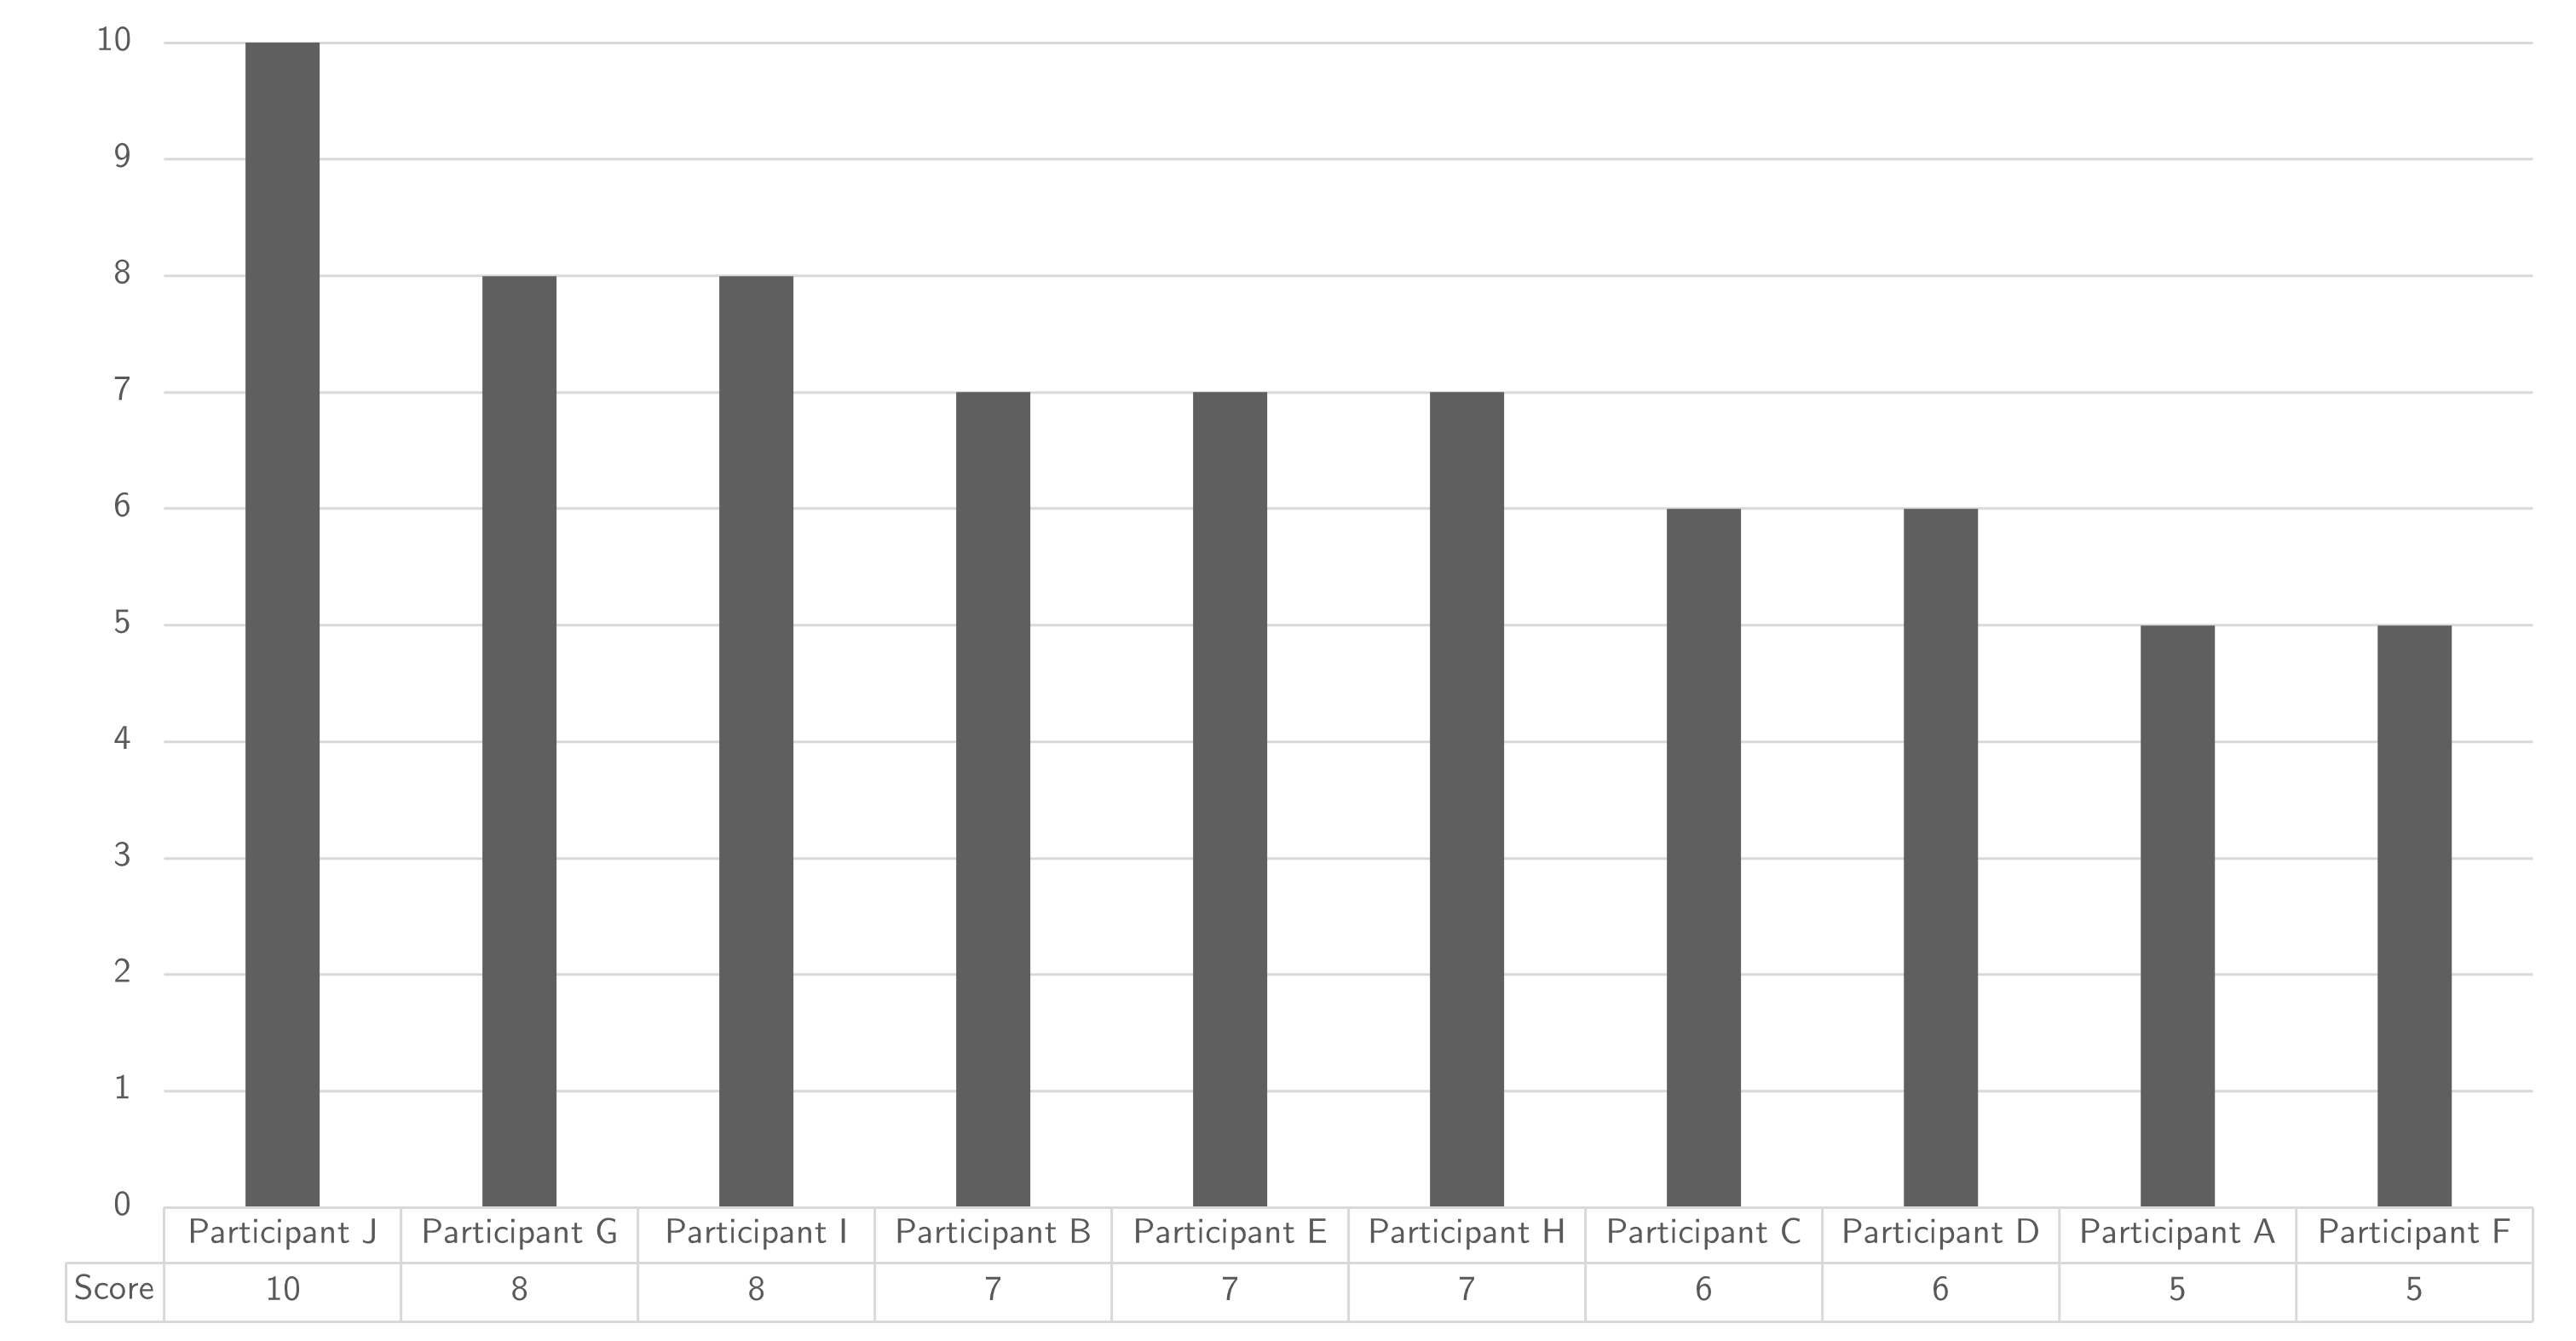
\includegraphics[width=0.9\linewidth]{images/scoreafoptionality}
	\caption[Scoring of antifragile attribute Optionality]{Scoring of antifragile attribute Optionality}
	\label{fig:appscoringafoptionality}
\end{figure}
\begin{table}[h!]
	\centering
	\begin{tabular}{p{.55\textwidth}ccc}
		\toprule
		\textbf{Attribute} & \textbf{Rating} & \textbf{Variability} & \textbf{Abstains} \\
		\midrule
		Optionality & 6,9 & 32\% & 0 \\%
		\bottomrule
	\end{tabular}%
	\caption[Scoring of antifragile attribute Optionality]{Scoring of antifragile attribute Optionality}
	\label{tab:appscoringafoptionality}%
\end{table}%
\newpage
\subsection{Mono-Monotonicity}
\begin{figure}[h!]
	\centering
	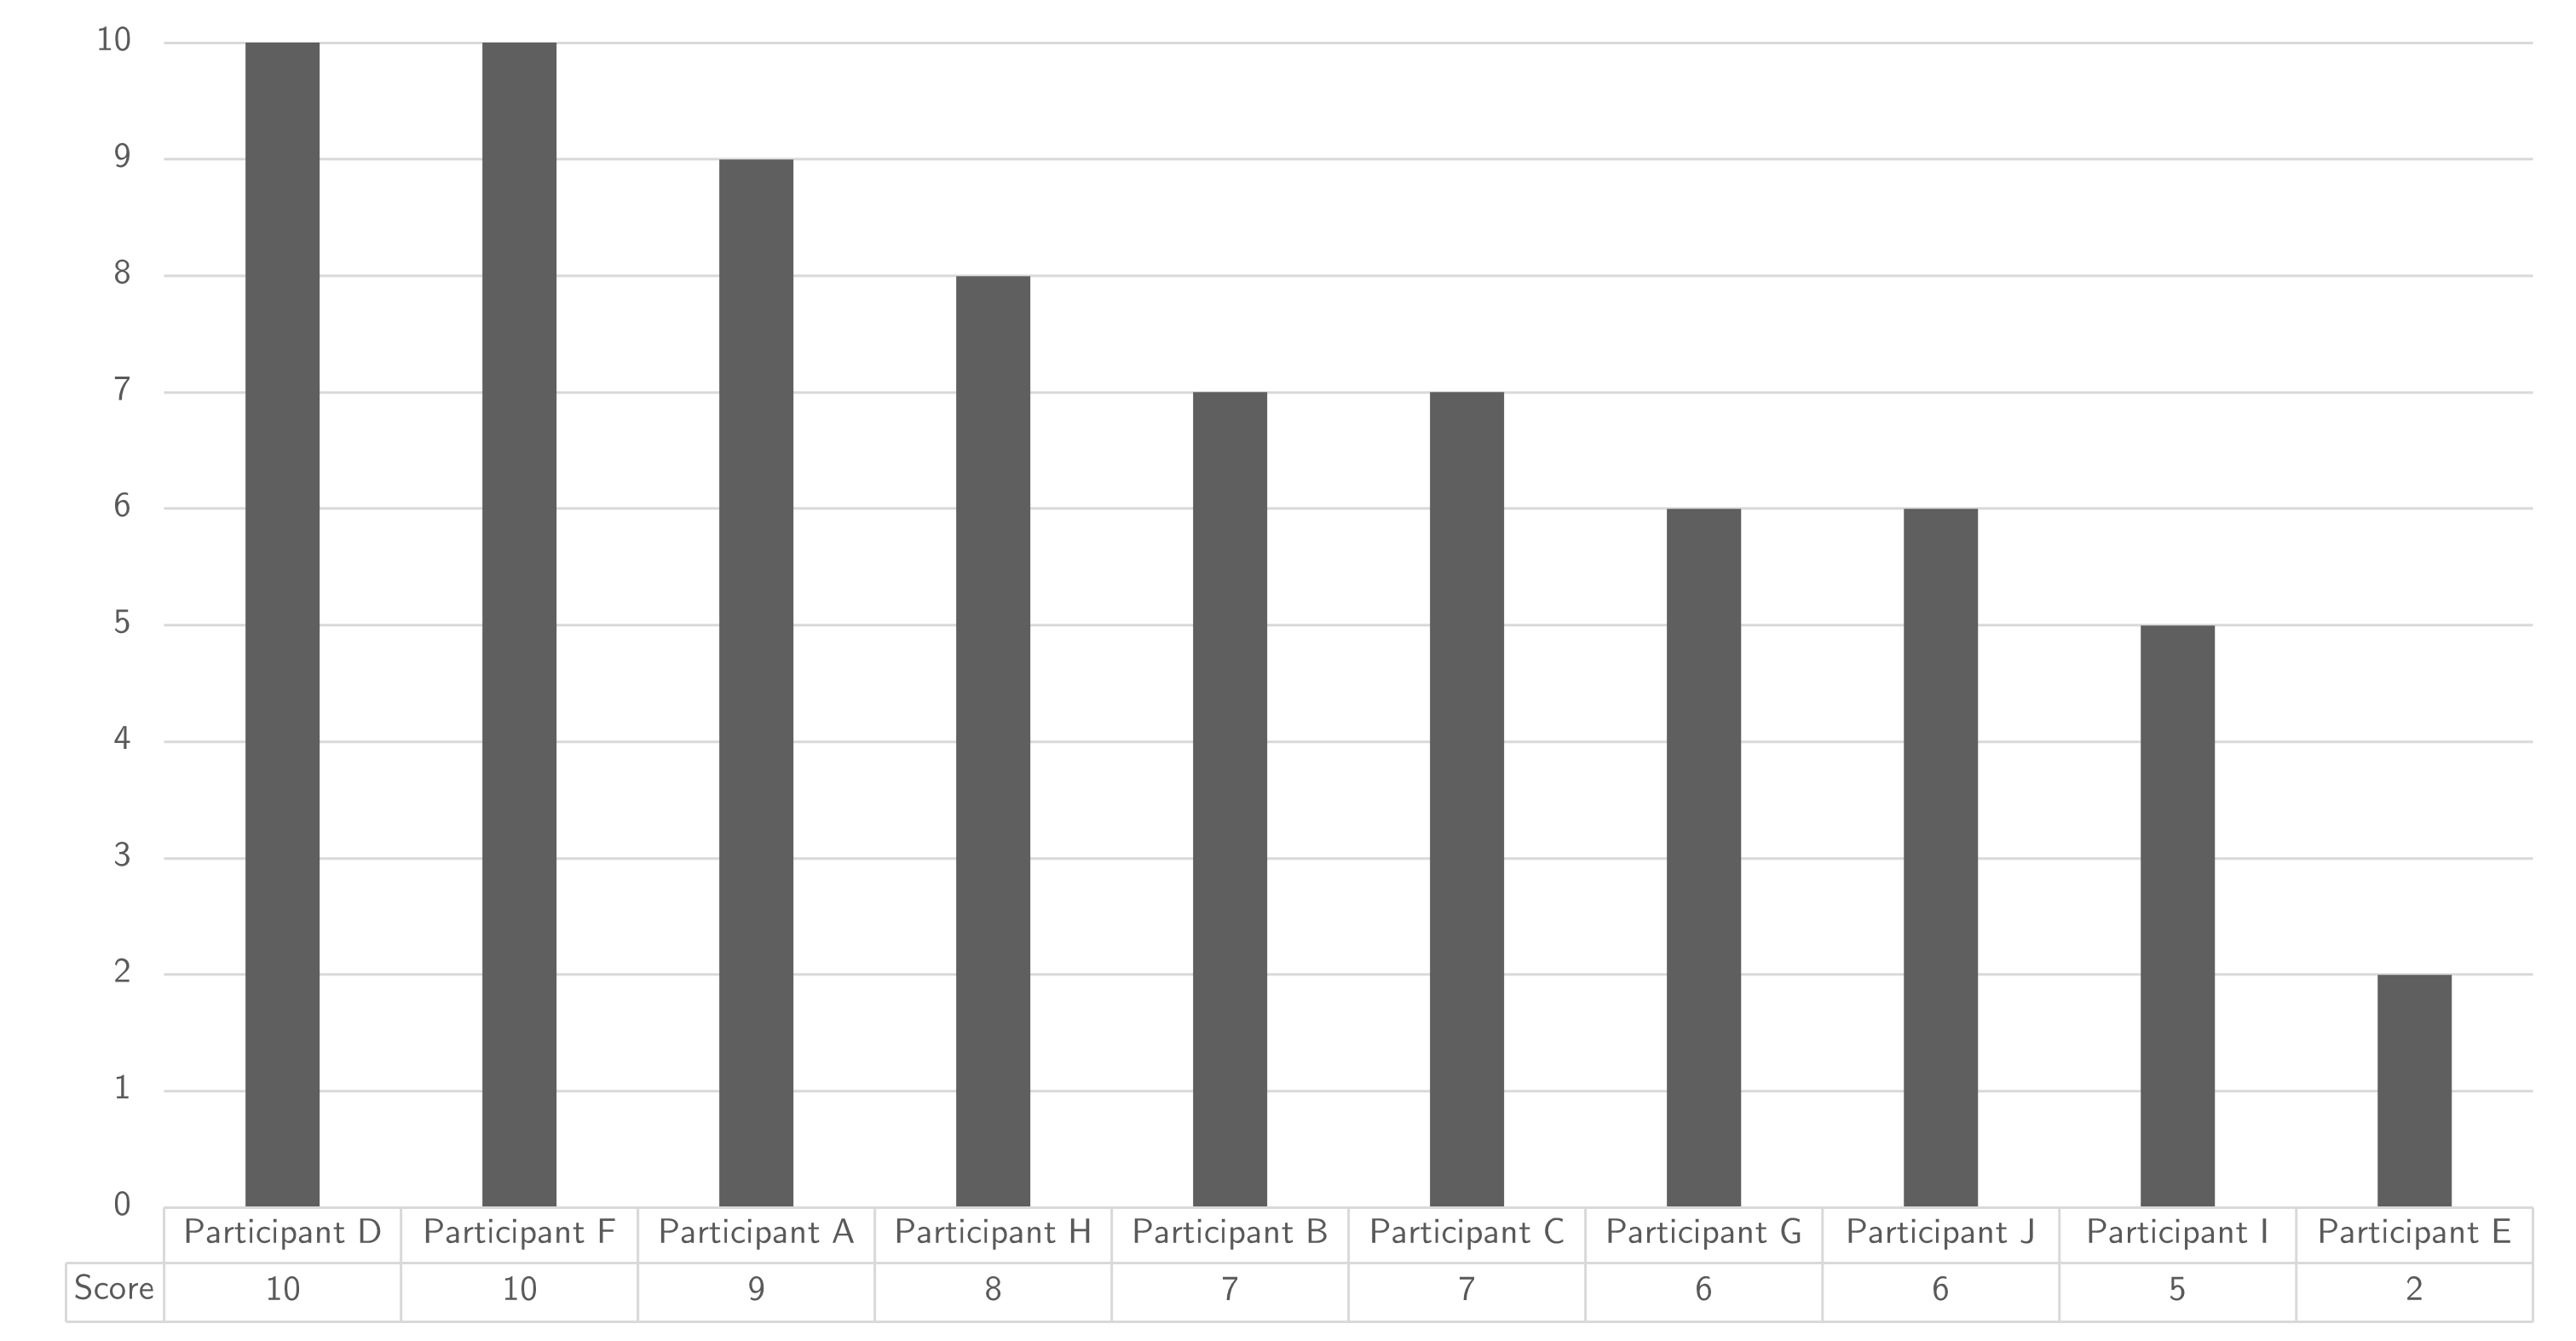
\includegraphics[width=0.9\linewidth]{images/scoreafmonomonotonicity}
	\caption[Scoring of antifragile attribute Mono-Monotonicity]{Scoring of antifragile attribute Mono-Monotonicity}
	\label{fig:appscoringafmonomonotonicity}
\end{figure}
\begin{table}[h!]
	\centering
	\begin{tabular}{p{.55\textwidth}ccc}
		\toprule
		\textbf{Attribute} & \textbf{Rating} & \textbf{Variability} & \textbf{Abstains} \\
		\midrule
		Mono-Monotonicity & 7 & 51\% & 0 \\%
		\bottomrule
	\end{tabular}%
	\caption[Scoring of antifragile attribute Mono-Monotonicity]{Scoring of antifragile attribute Mono-Monotonicity}
	\label{tab:appscoringafmonomonotonicity}%
\end{table}%
\newpage
\subsection{Self-Organisation}
\begin{figure}[h!]
	\centering
	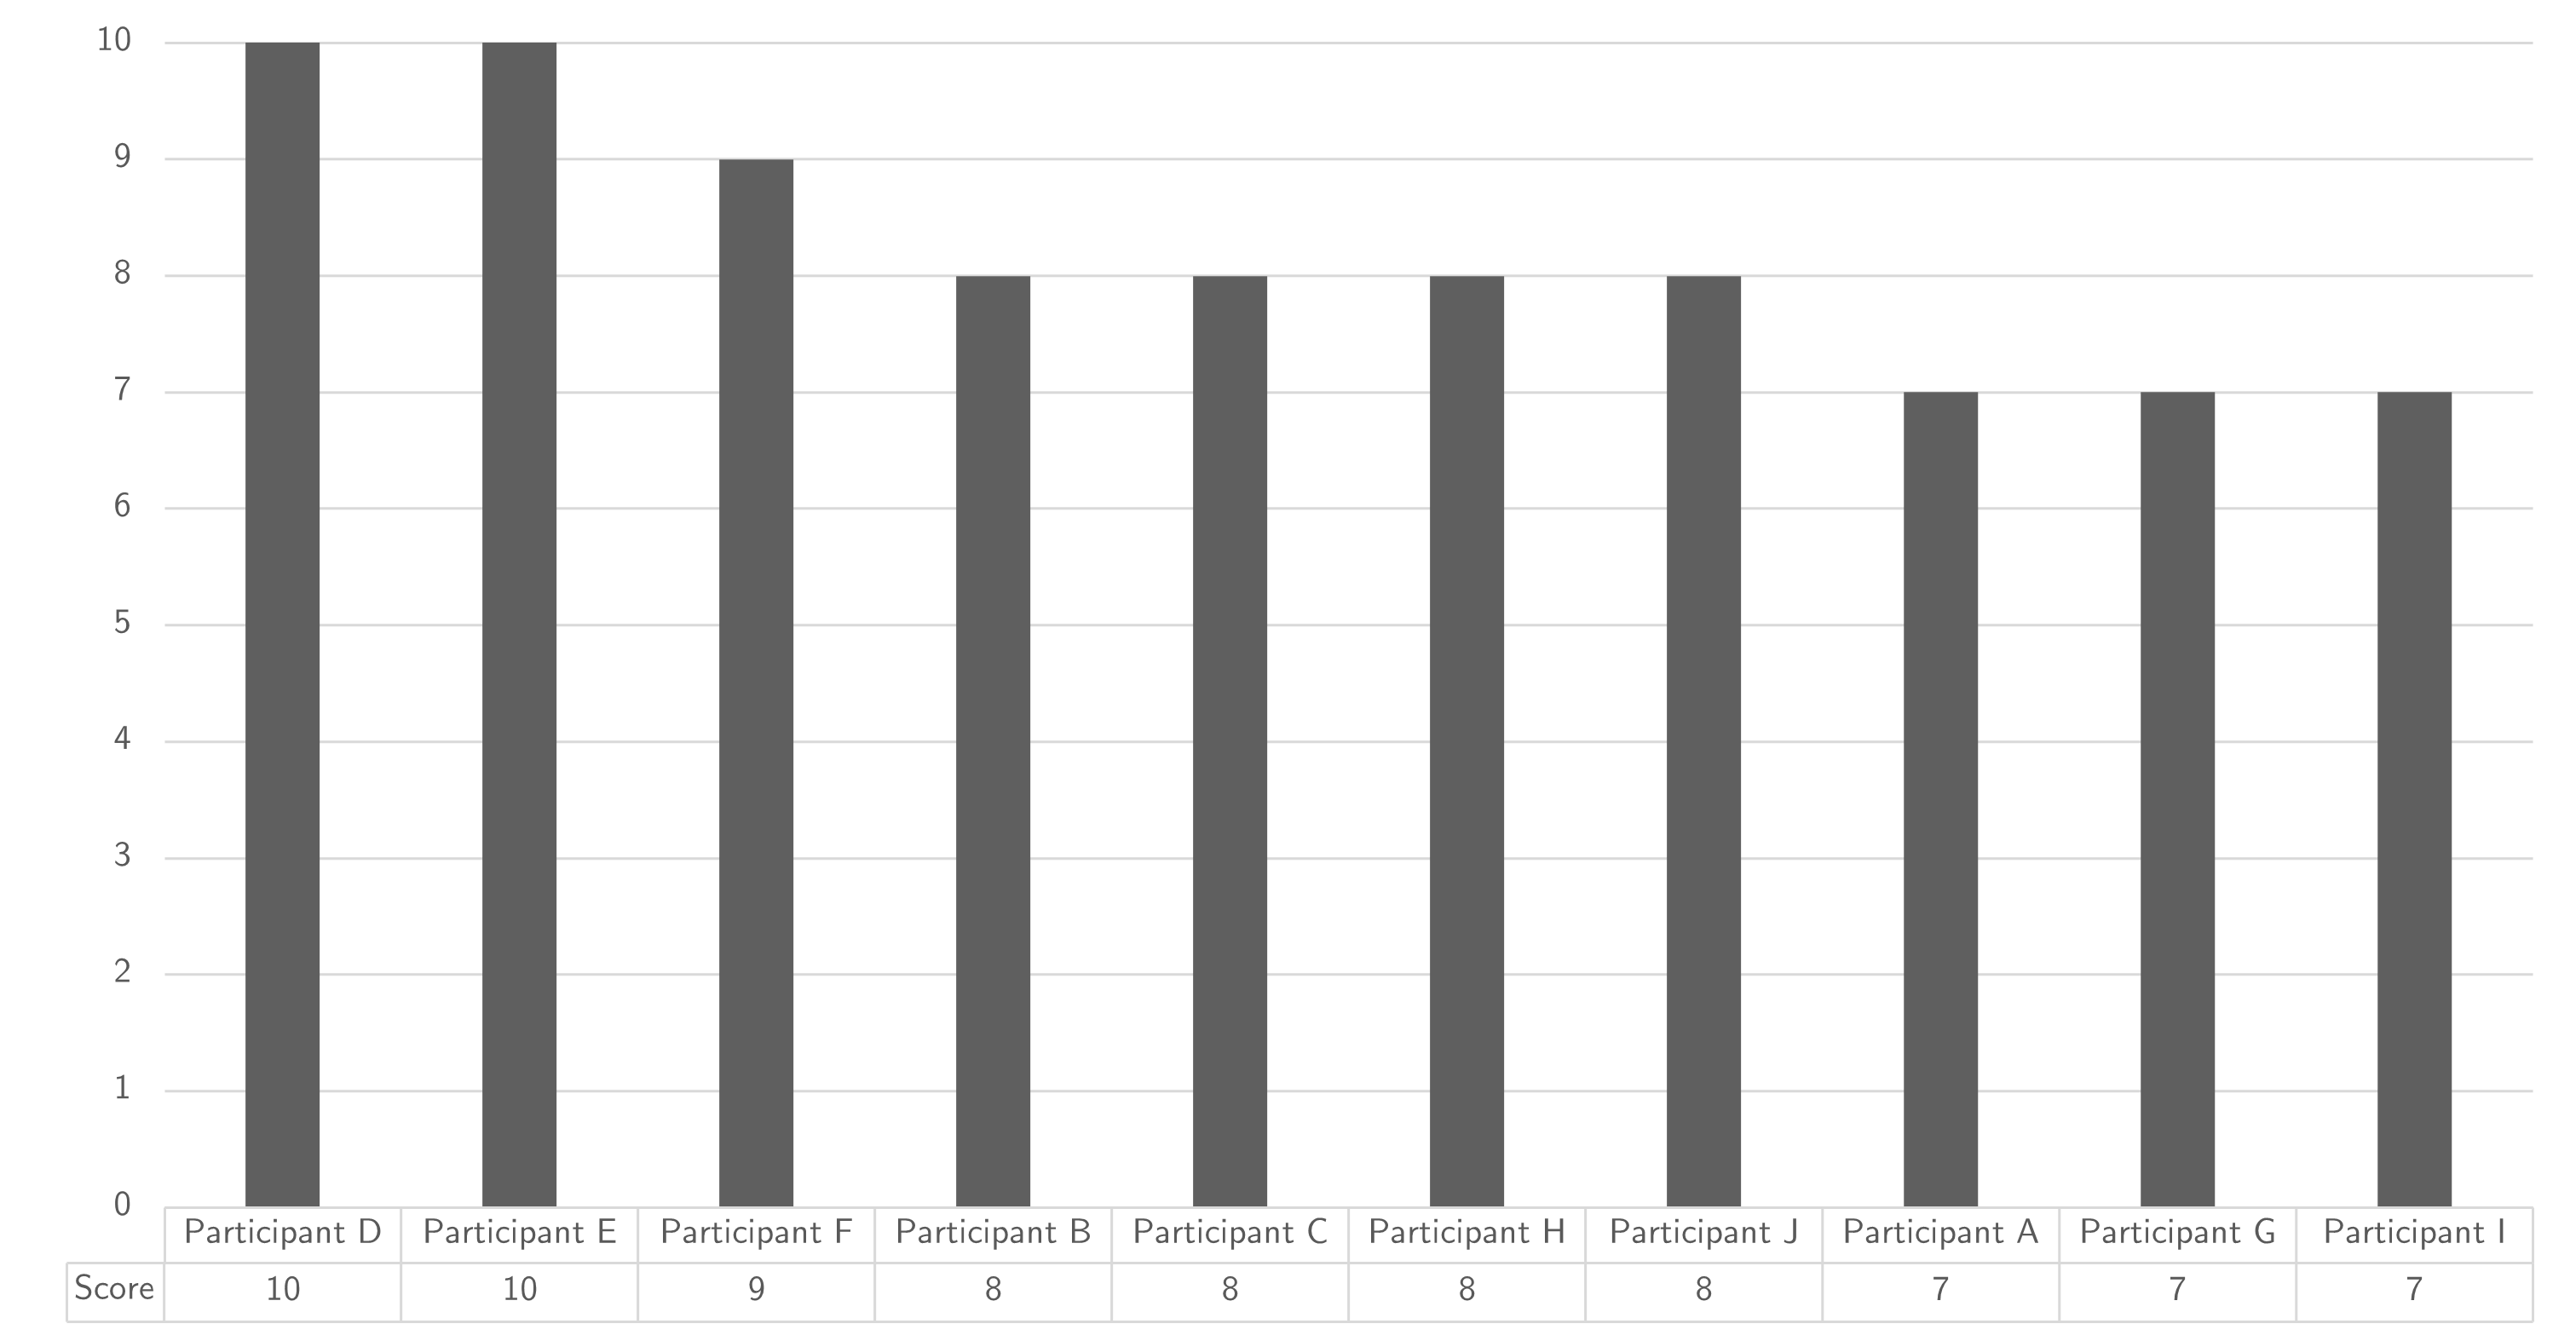
\includegraphics[width=0.9\linewidth]{images/scoreafselforganisation}
	\caption[Scoring of antifragile attribute Self-Organisation]{Scoring of antifragile attribute Self-Organisation}
	\label{fig:appscoringafselforganisation}
\end{figure}
\begin{table}[h!]
	\centering
	\begin{tabular}{p{.55\textwidth}ccc}
		\toprule
		\textbf{Attribute} & \textbf{Rating} & \textbf{Variability} & \textbf{Abstains} \\
		\midrule
		Self-Organisation & 8,2 & 23\% & 0 \\%
		\bottomrule
	\end{tabular}%
	\caption[Scoring of antifragile attribute Self-Organisation]{Scoring of antifragile attribute Self-Organisation}
	\label{tab:appscoringafselforganisation}%
\end{table}%
\newpage
\subsection{Fail-Fast}
\begin{figure}[h!]
	\centering
	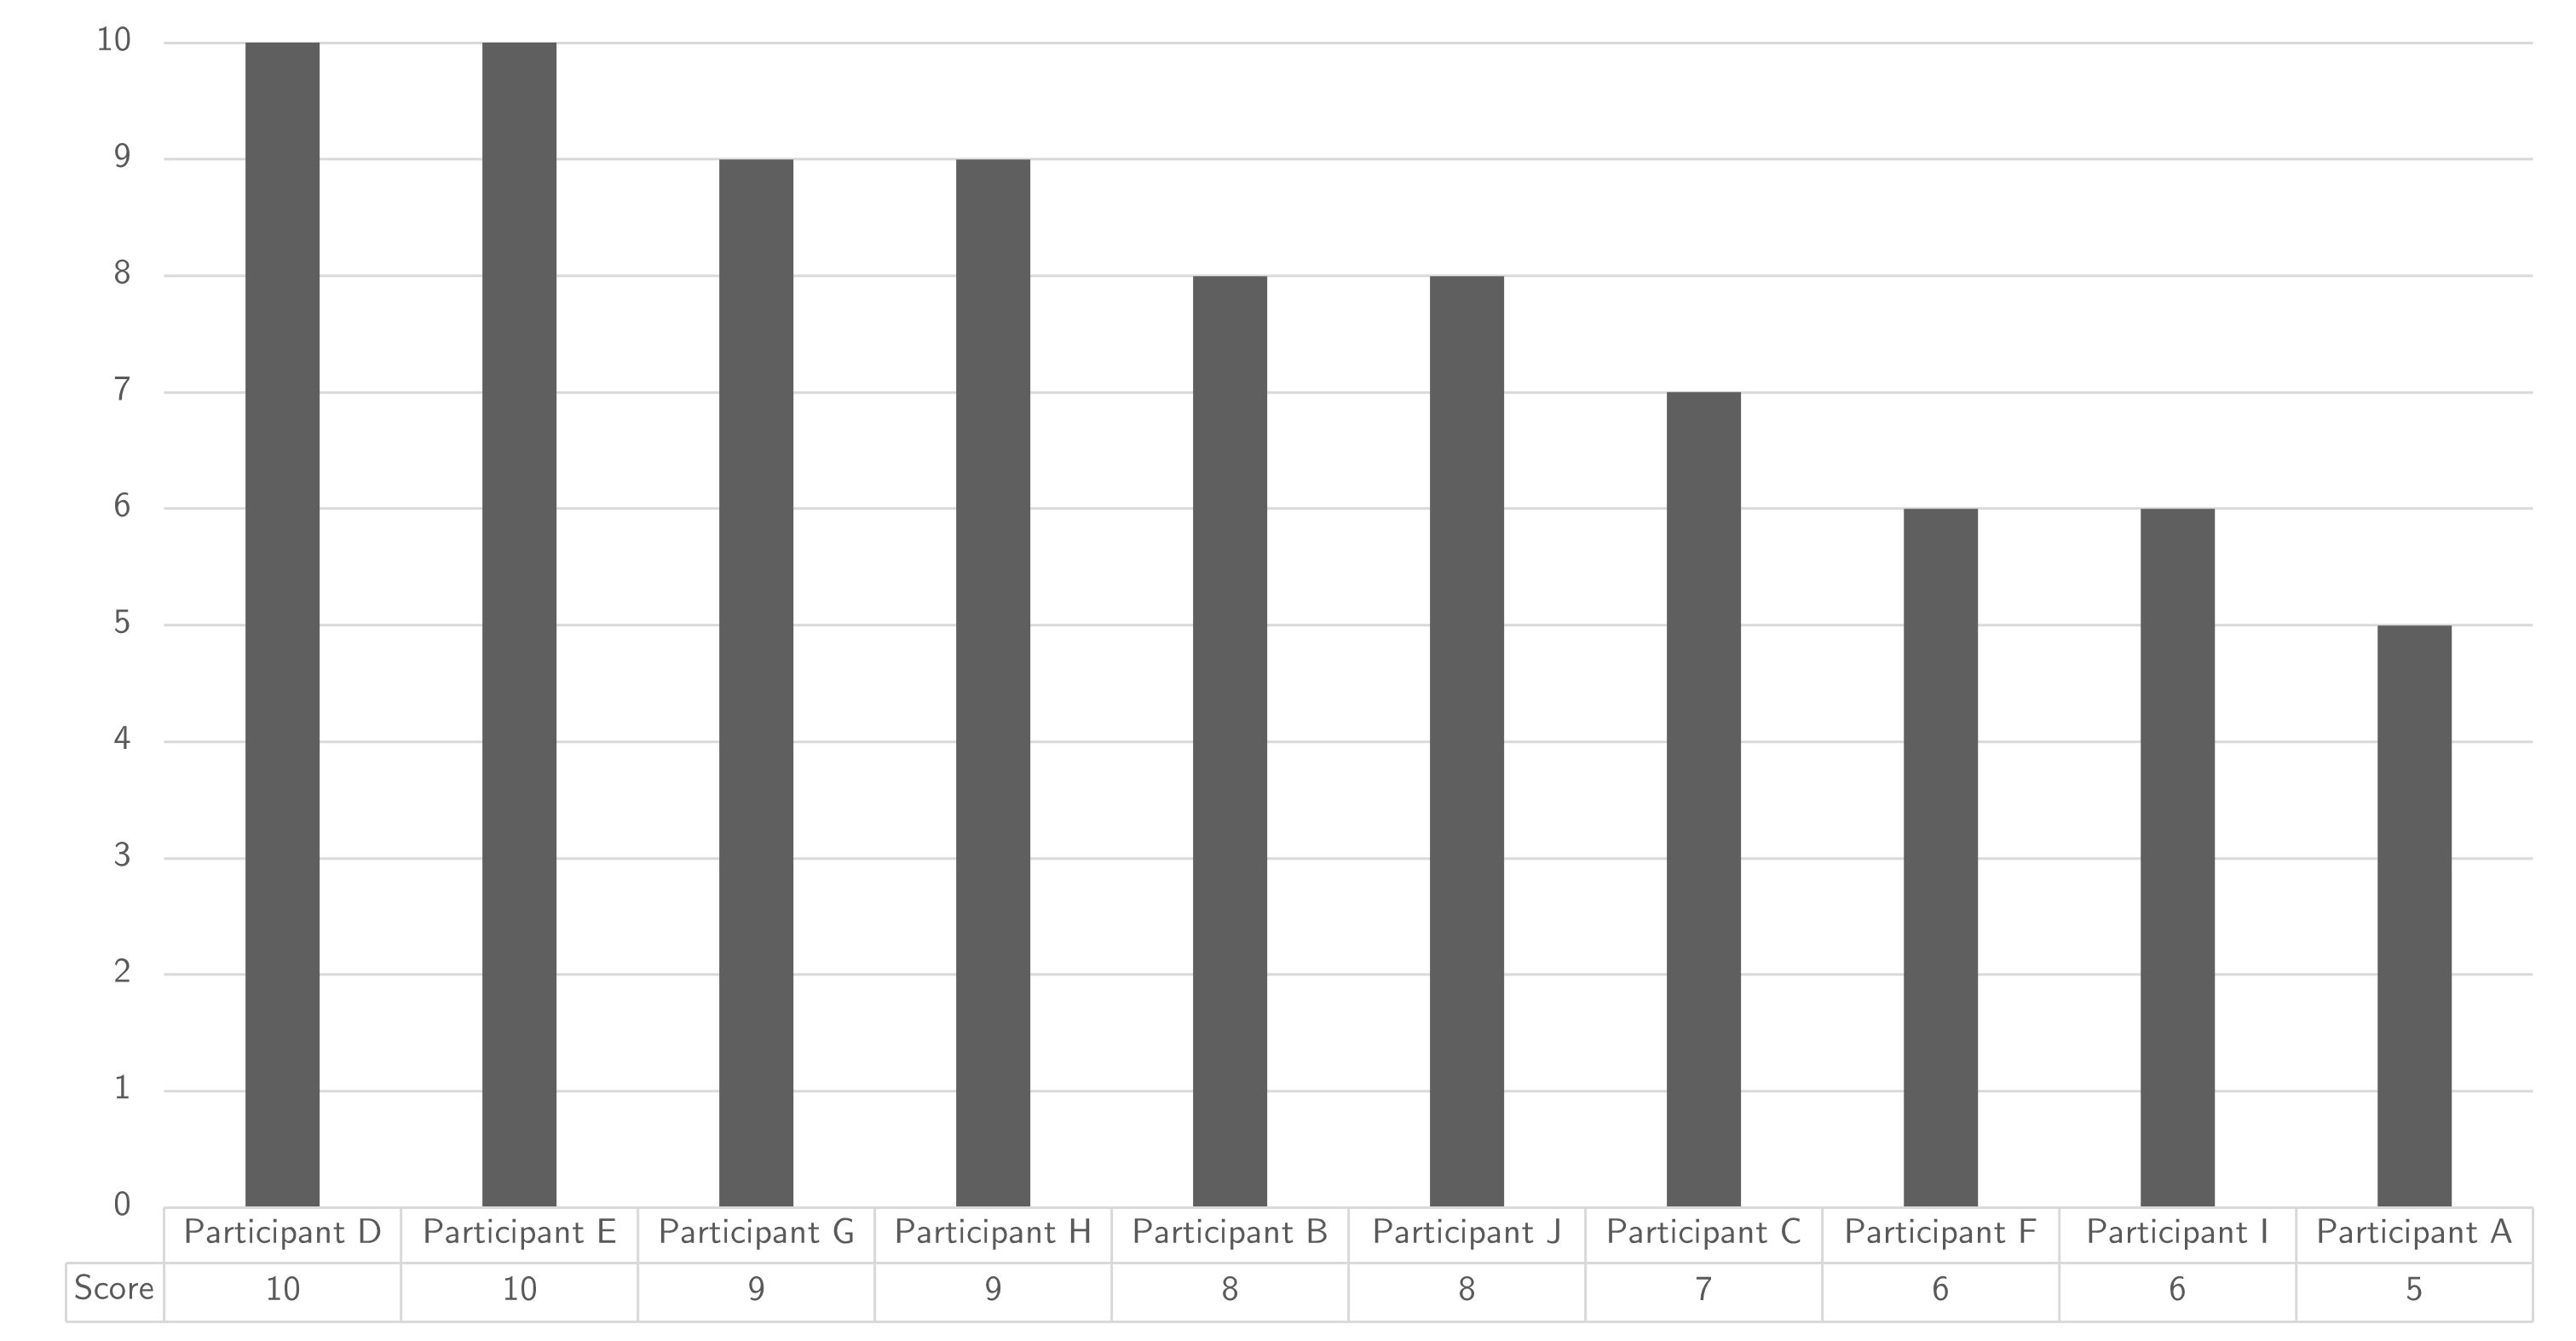
\includegraphics[width=0.9\linewidth]{images/scoreaffailfast}
	\caption[Scoring of antifragile attribute Fail-Fast]{Scoring of antifragile attribute Fail-Fast}
	\label{fig:appscoringaffailfast}
\end{figure}
\begin{table}[h!]
	\centering
	\begin{tabular}{p{.55\textwidth}ccc}
		\toprule
		\textbf{Attribute} & \textbf{Rating} & \textbf{Variability} & \textbf{Abstains} \\
		\midrule
		Fail-Fast & 7,8 & 35\% & 0 \\%
		\bottomrule
	\end{tabular}%
	\caption[Scoring of antifragile attribute Fail-Fast]{Scoring of antifragile attribute Fail-Fast}
	\label{tab:appscoringaffailfast}%
\end{table}%
\newpage
\subsection{Resources to invest}
\begin{figure}[h!]
	\centering
	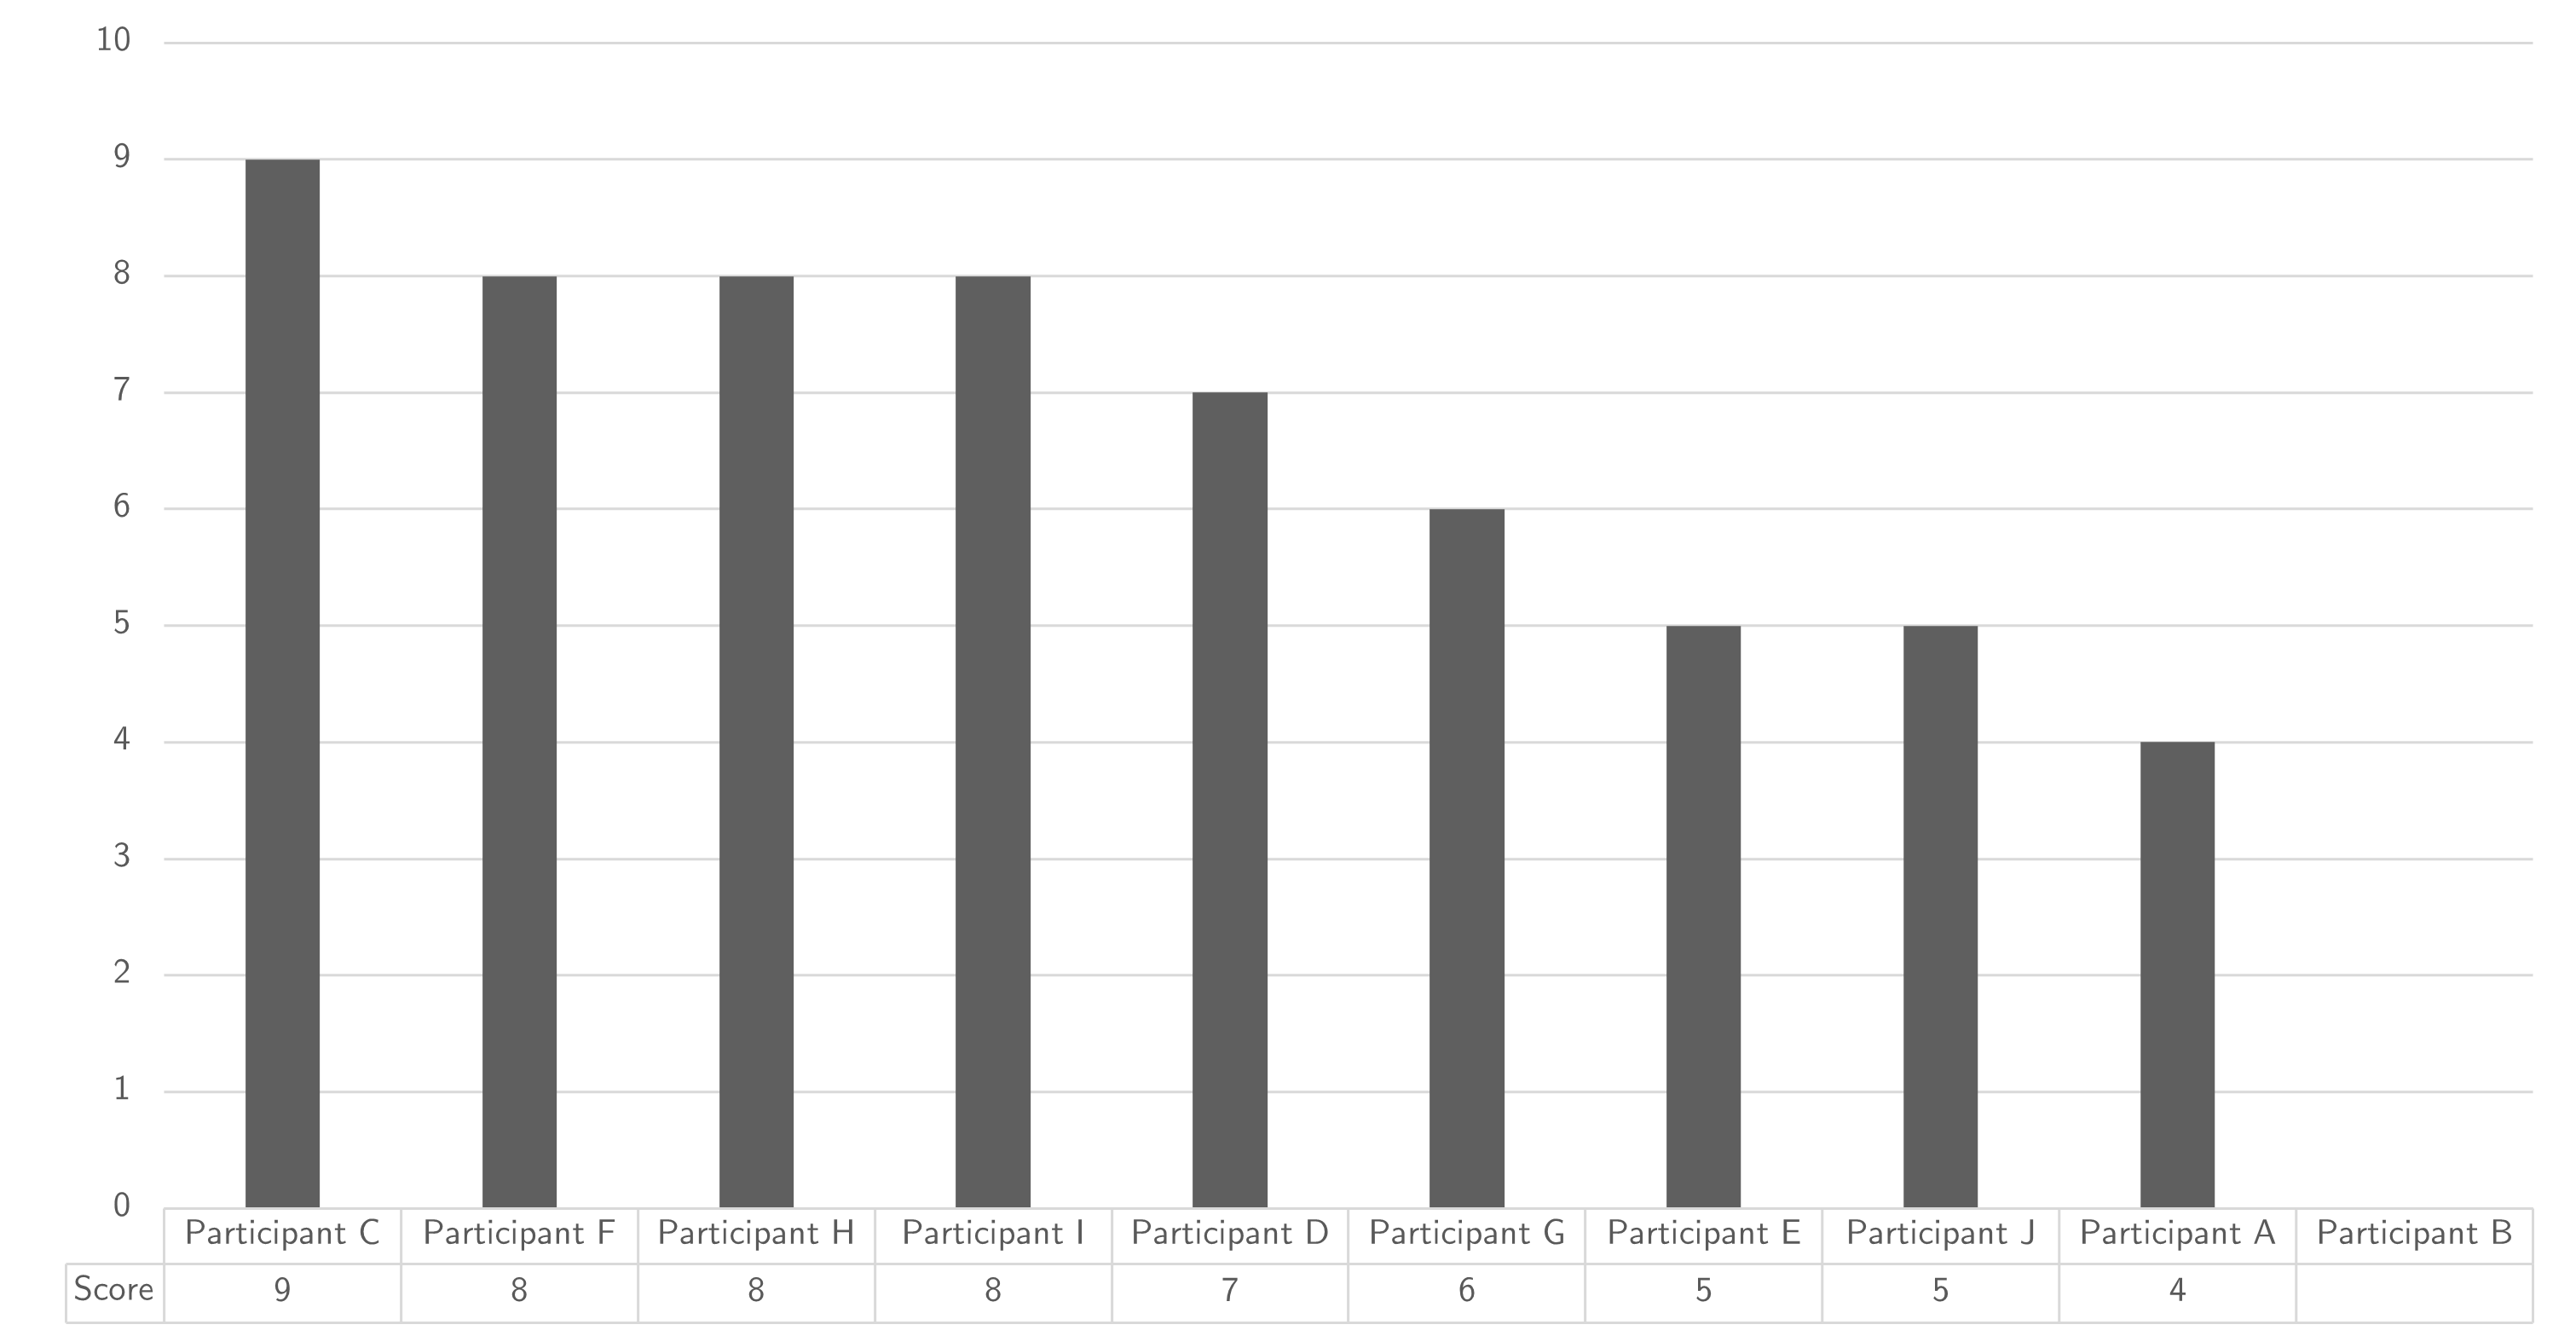
\includegraphics[width=0.9\linewidth]{images/scoreafresourcestoinvest}
	\caption[Scoring of antifragile attribute Resources to Invest]{Scoring of antifragile attribute Resources to Invest}
	\label{fig:appscoringafresourcestoinvest}
\end{figure}
\begin{table}[h!]
	\centering
	\begin{tabular}{p{.55\textwidth}ccc}
		\toprule
		\textbf{Attribute} & \textbf{Rating} & \textbf{Variability} & \textbf{Abstains} \\
		\midrule
		Resources to Invest & 6,7 & 36\% & 1 \\%
		\bottomrule
	\end{tabular}%
	\caption[Scoring of antifragile attribute Resources to Invest]{Scoring of antifragile attribute Resources to Invest}
	\label{tab:appscoringafresourcestoinvest}%
\end{table}%
\newpage
\subsection{Senenca's Barbell}
\begin{figure}[h!]
	\centering
	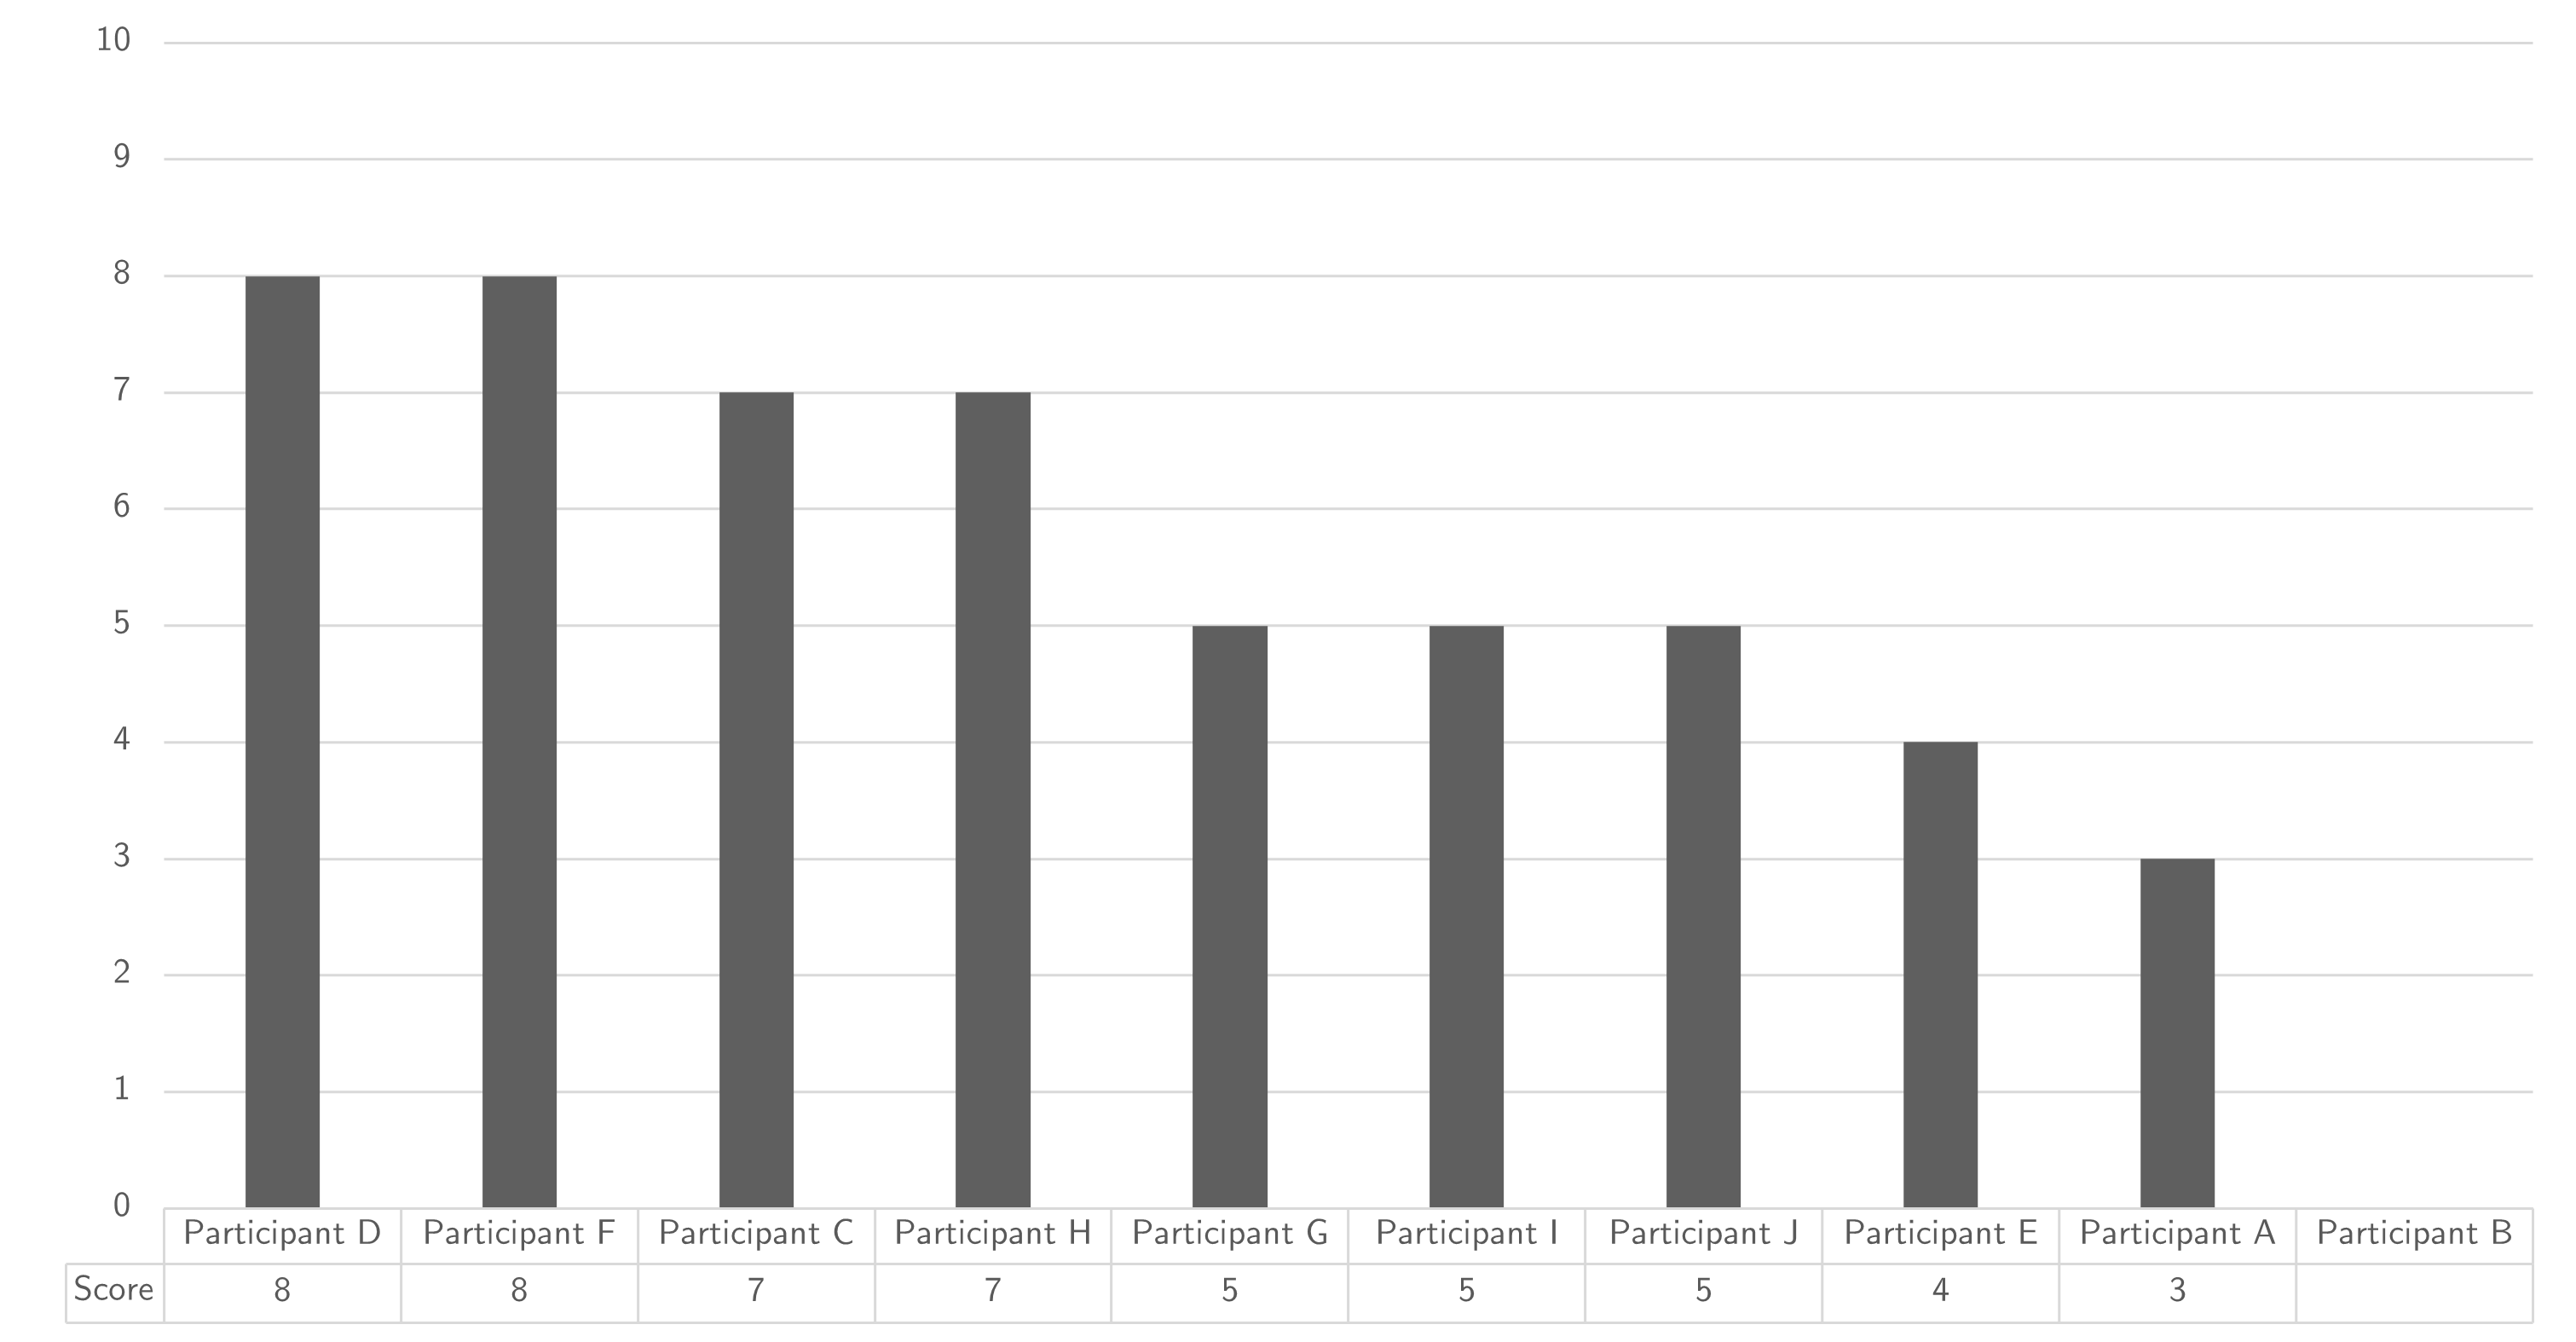
\includegraphics[width=0.9\linewidth]{images/scoreafseneca}
	\caption[Scoring of antifragile attribute Seneca's Barbell]{Scoring of antifragile attribute Seneca's Barbell}
	\label{fig:appscoringafseneca}
\end{figure}
\begin{table}[h!]
	\centering
	\begin{tabular}{p{.55\textwidth}ccc}
		\toprule
		\textbf{Attribute} & \textbf{Rating} & \textbf{Variability} & \textbf{Abstains} \\
		\midrule
		Seneca's Barbell & 5,8 & 37\% & 1 \\%
		\bottomrule
	\end{tabular}%
	\caption[Scoring of antifragile attribute Seneca's Barbell]{Scoring of antifragile attribute Seneca's Barbell}
	\label{tab:appscoringafseneca}%
\end{table}%
\newpage
\subsection{Safe working environment}
\begin{figure}[h!]
	\centering
	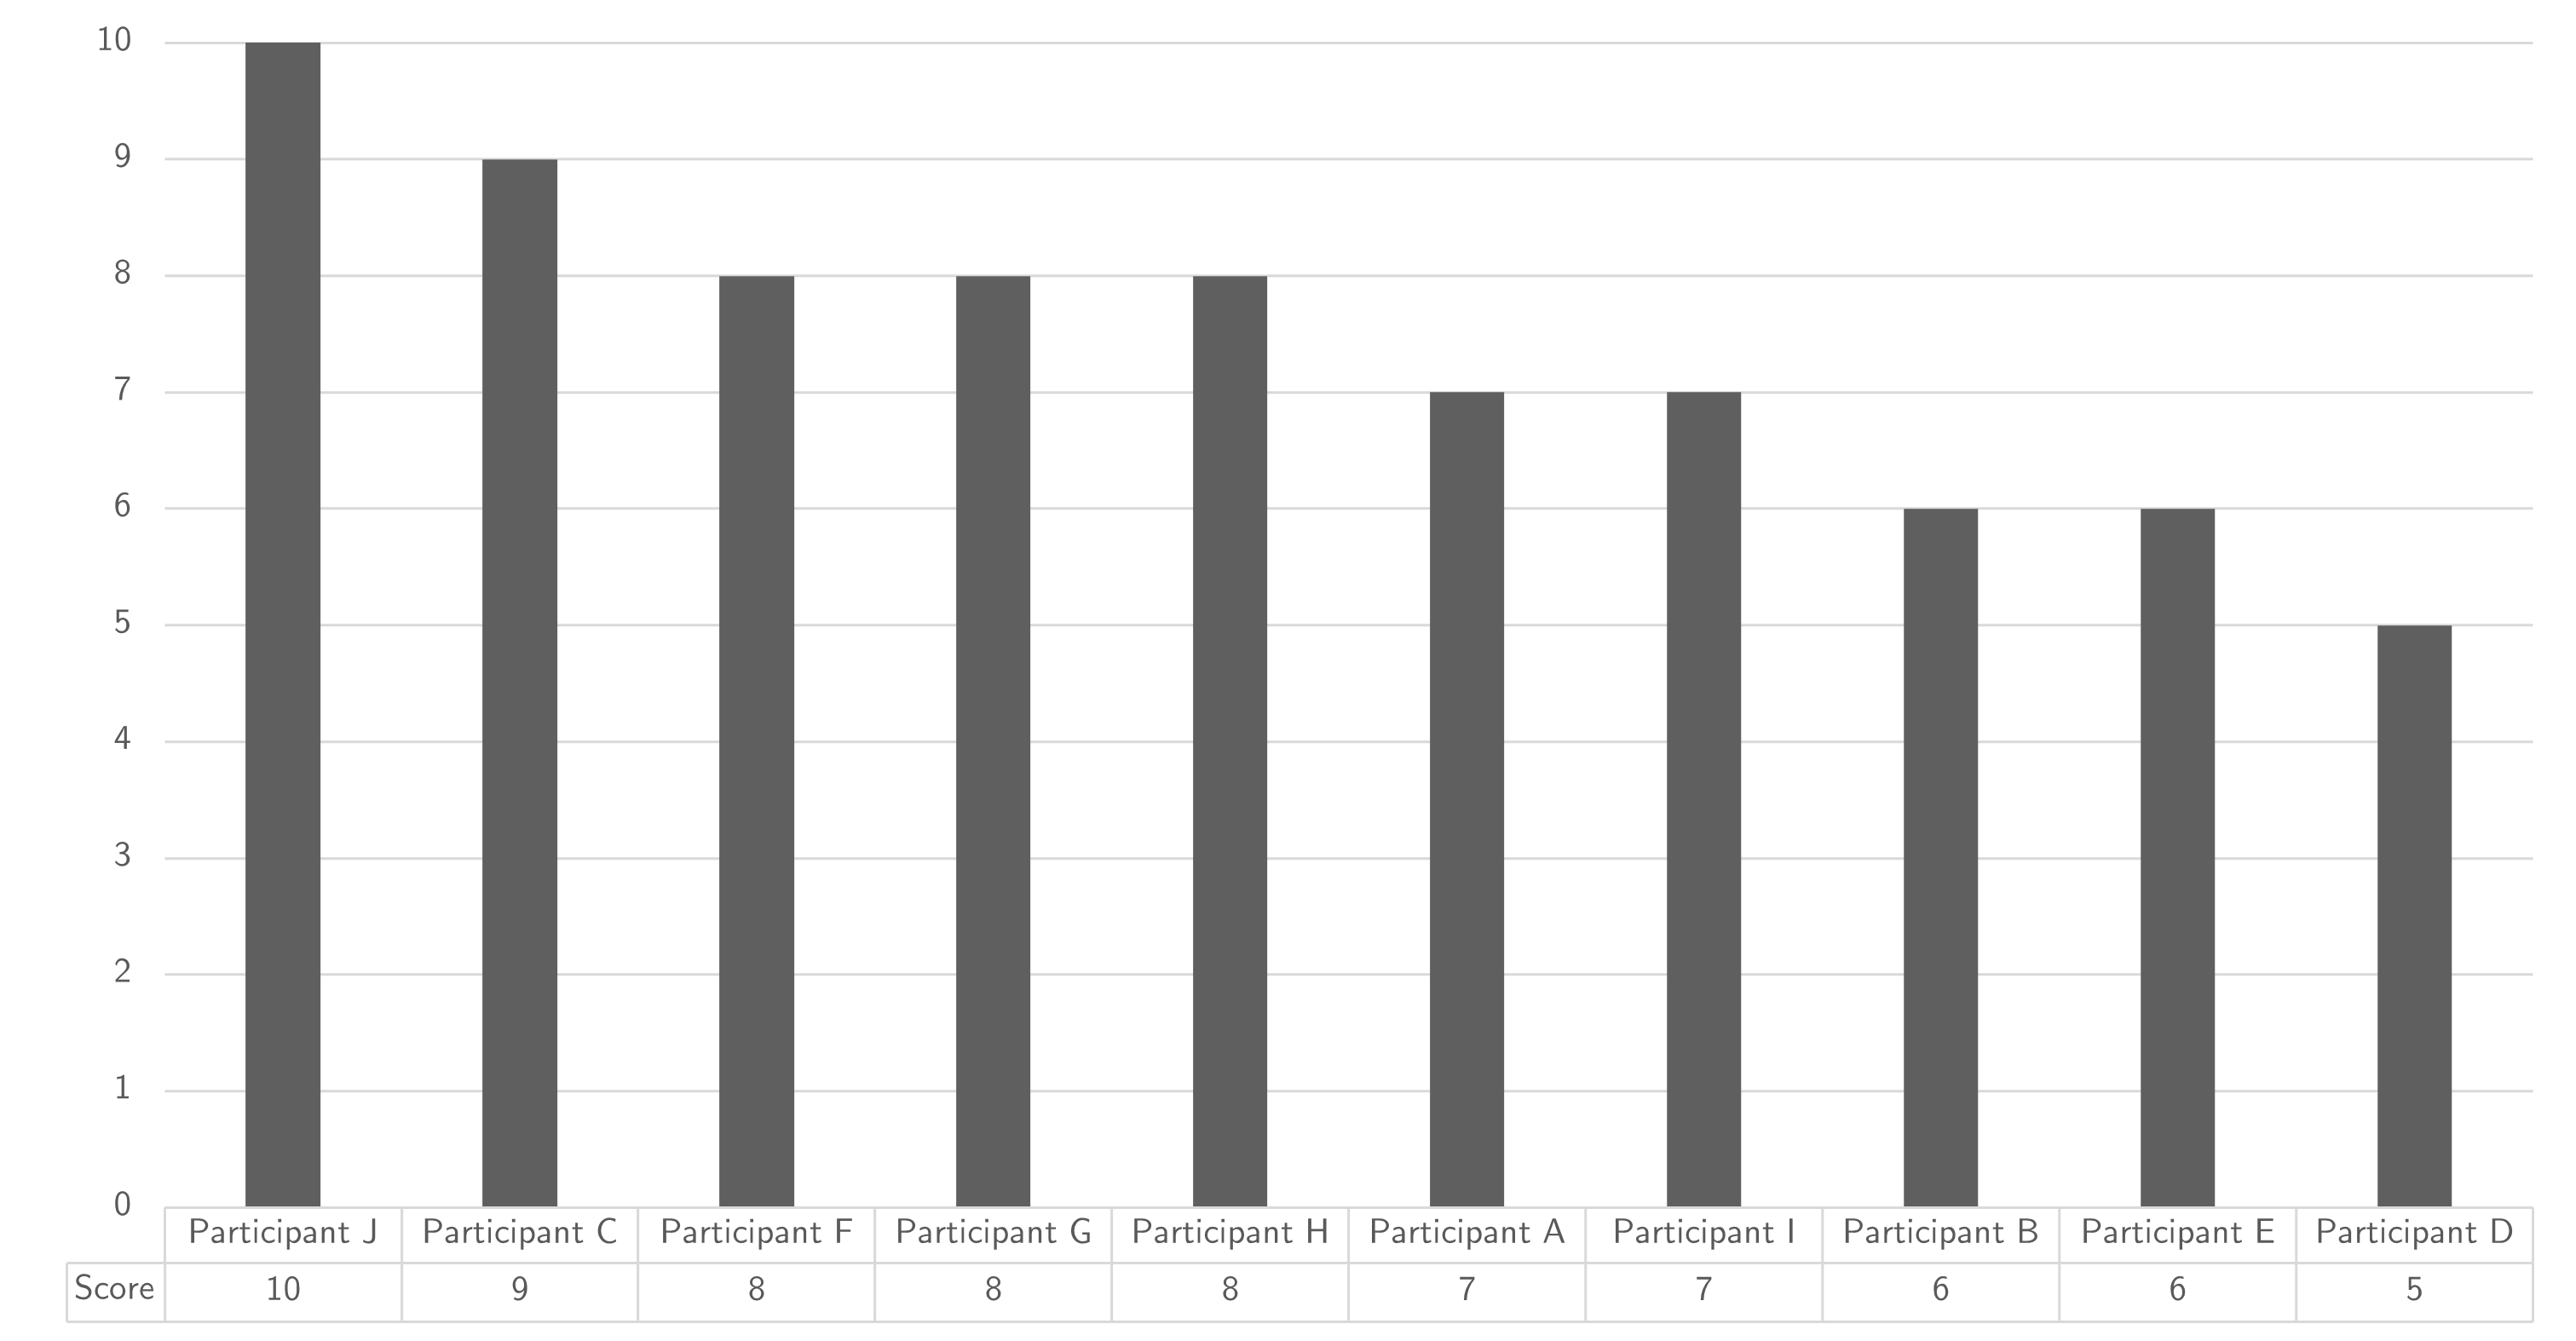
\includegraphics[width=0.9\linewidth]{images/scoreafsafeworkingenvironnment}
	\caption[Scoring of antifragile attribute Safe working environment]{Scoring of antifragile attribute Safe working environment}
	\label{fig:appscoringafsafeworkingenvironnment}
\end{figure}
\begin{table}[h!]
	\centering
	\begin{tabular}{p{.55\textwidth}ccc}
		\toprule
		\textbf{Attribute} & \textbf{Rating} & \textbf{Variability} & \textbf{Abstains} \\
		\midrule
		Safe working environment & 7,4 & 31\% & 0 \\%
		\bottomrule
	\end{tabular}%
	\caption[Scoring of antifragile attribute Safe working environment]{Scoring of antifragile attribute Safe working environment}
	\label{tab:appscoringafsafeworkingenvironment}%
\end{table}%
\newpage
\subsection{Naar buiten kijken, samenwerking zoeken}
\begin{figure}[h!]
	\centering
	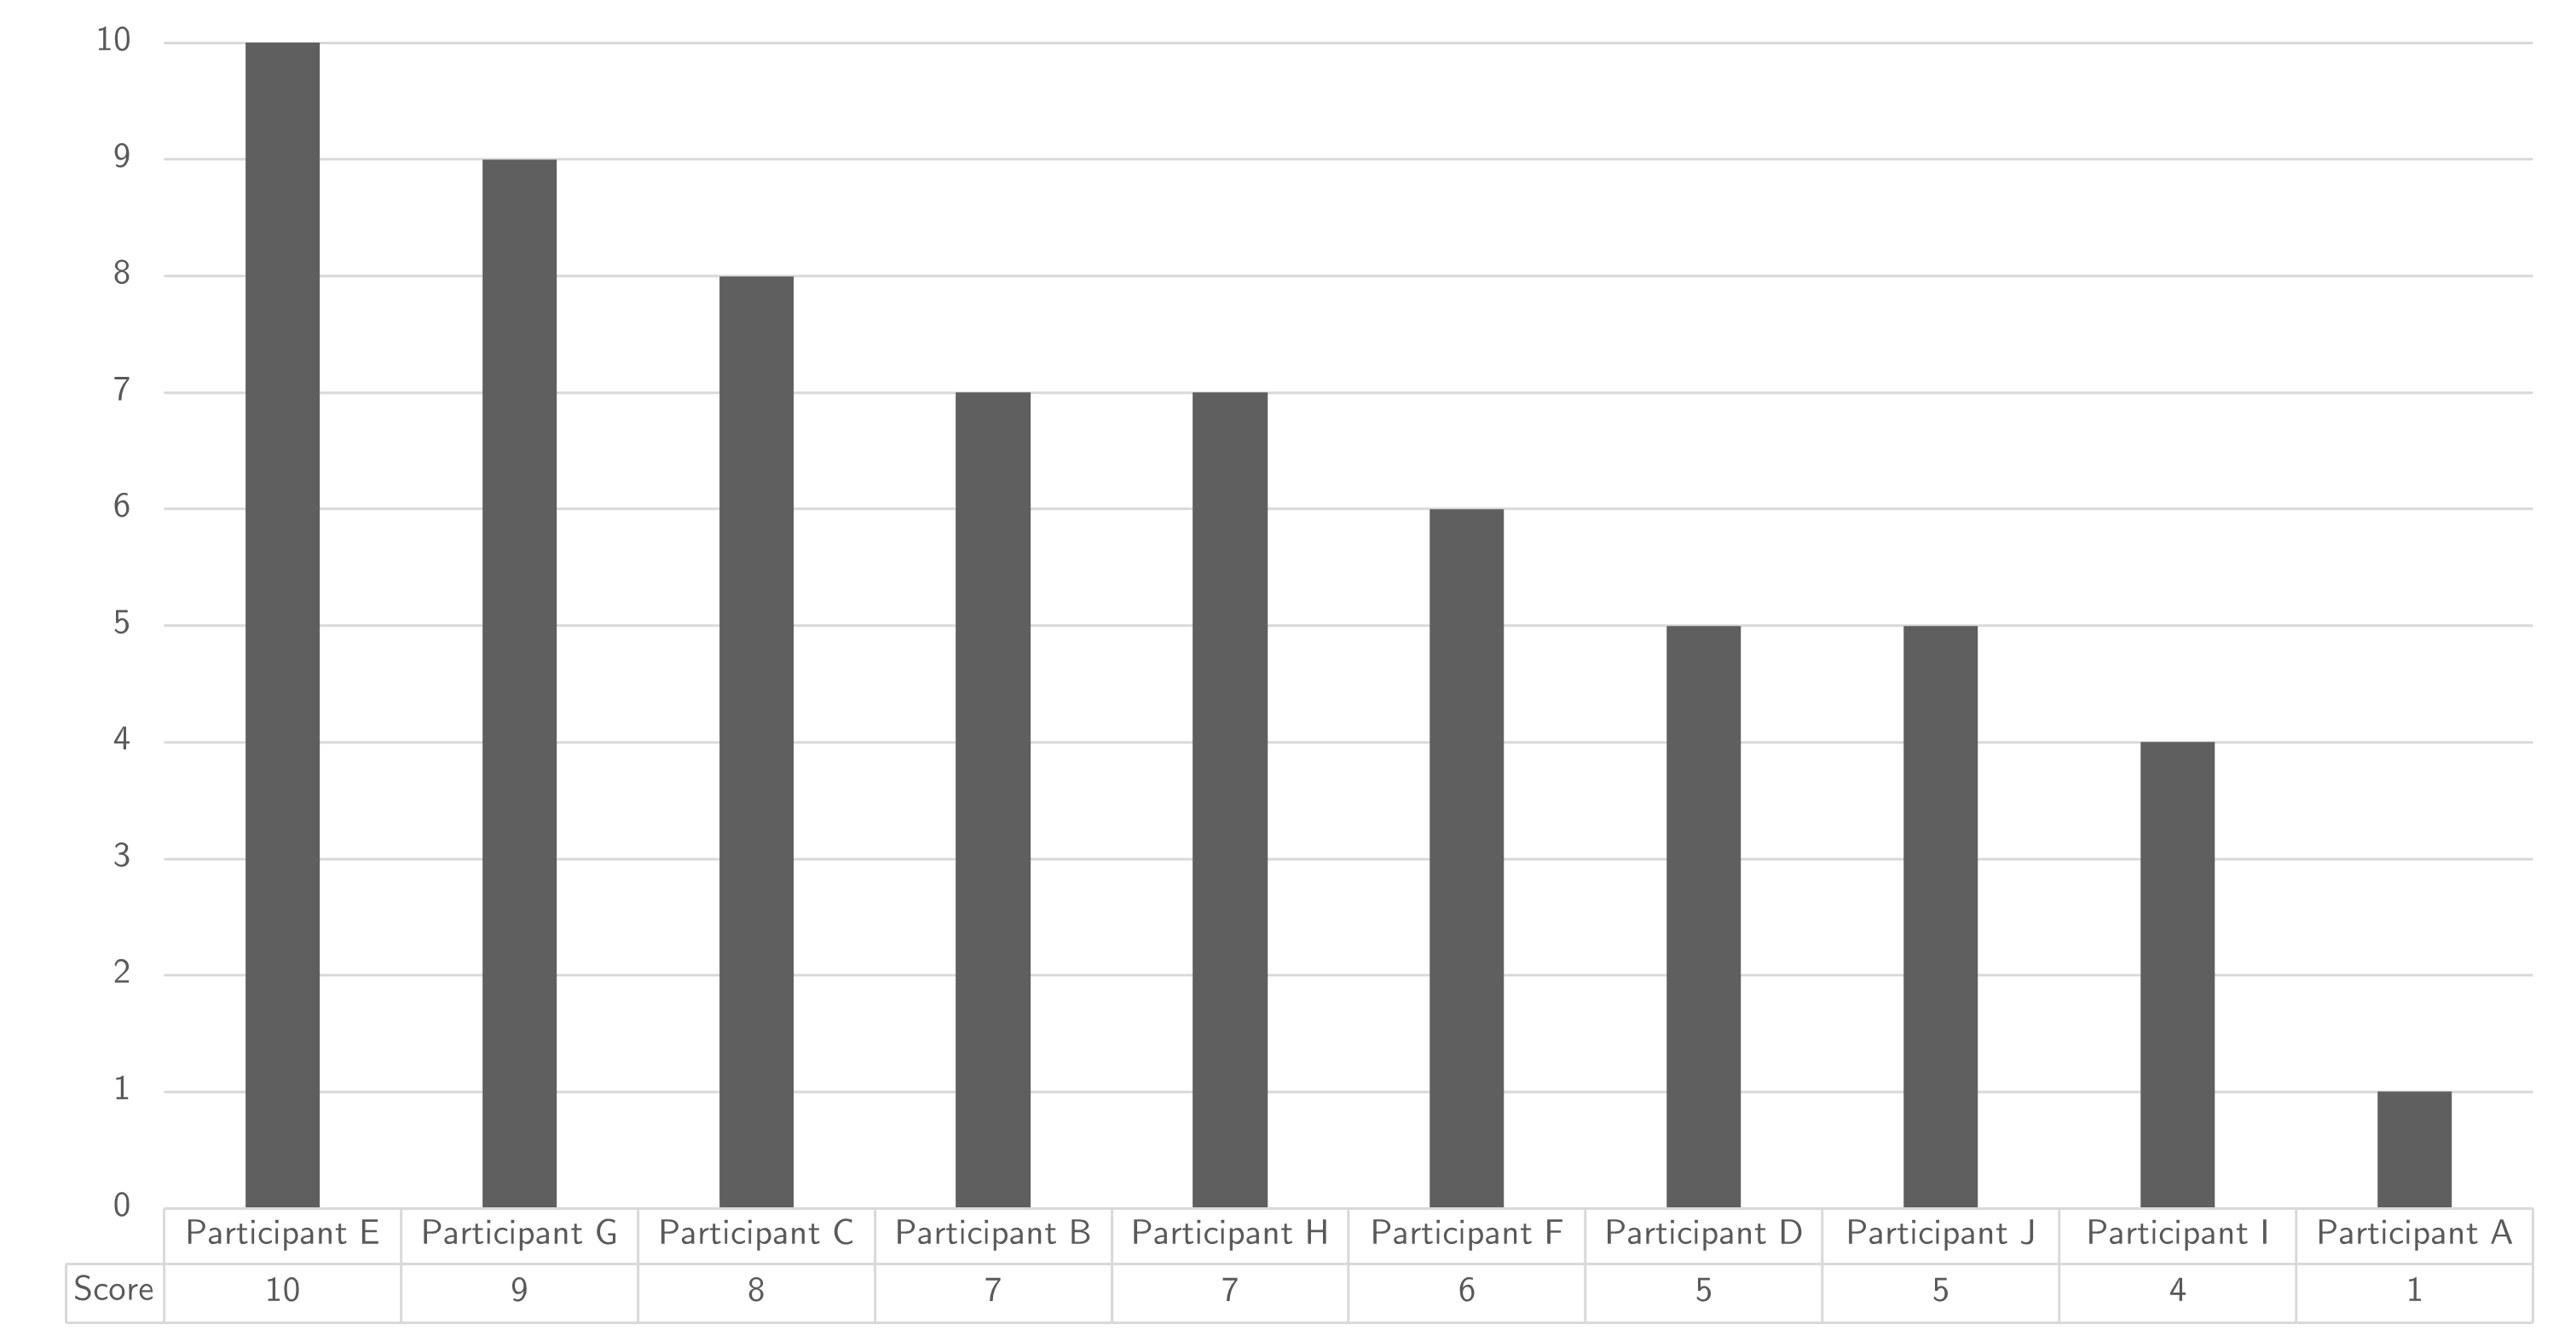
\includegraphics[width=0.9\linewidth]{images/scoreafnaarbuitenkijken}
	\caption[Scoring of antifragile attribute Naar buiten kijken]{Scoring of antifragile attribute Naar buiten kijken}
	\label{fig:appscoringafnaarbuiten}
\end{figure}
\begin{table}[h!]
	\centering
	\begin{tabular}{p{.55\textwidth}ccc}
		\toprule
		\textbf{Attribute} & \textbf{Rating} & \textbf{Variability} & \textbf{Abstains} \\
		\midrule
		Naar buiten kijken, samenwerking zoeken & 6,2 & 55\% & 0 \\%
		\bottomrule
	\end{tabular}%
	\caption[Scoring of antifragile attribute Naar buiten]{Scoring of antifragile attribute Naar buiten}
	\label{tab:appscoringafnaarbuitenkijken}%
\end{table}%
\newpage
\subsection{Data Governance Planes}
\begin{figure}[h!]
	\centering
	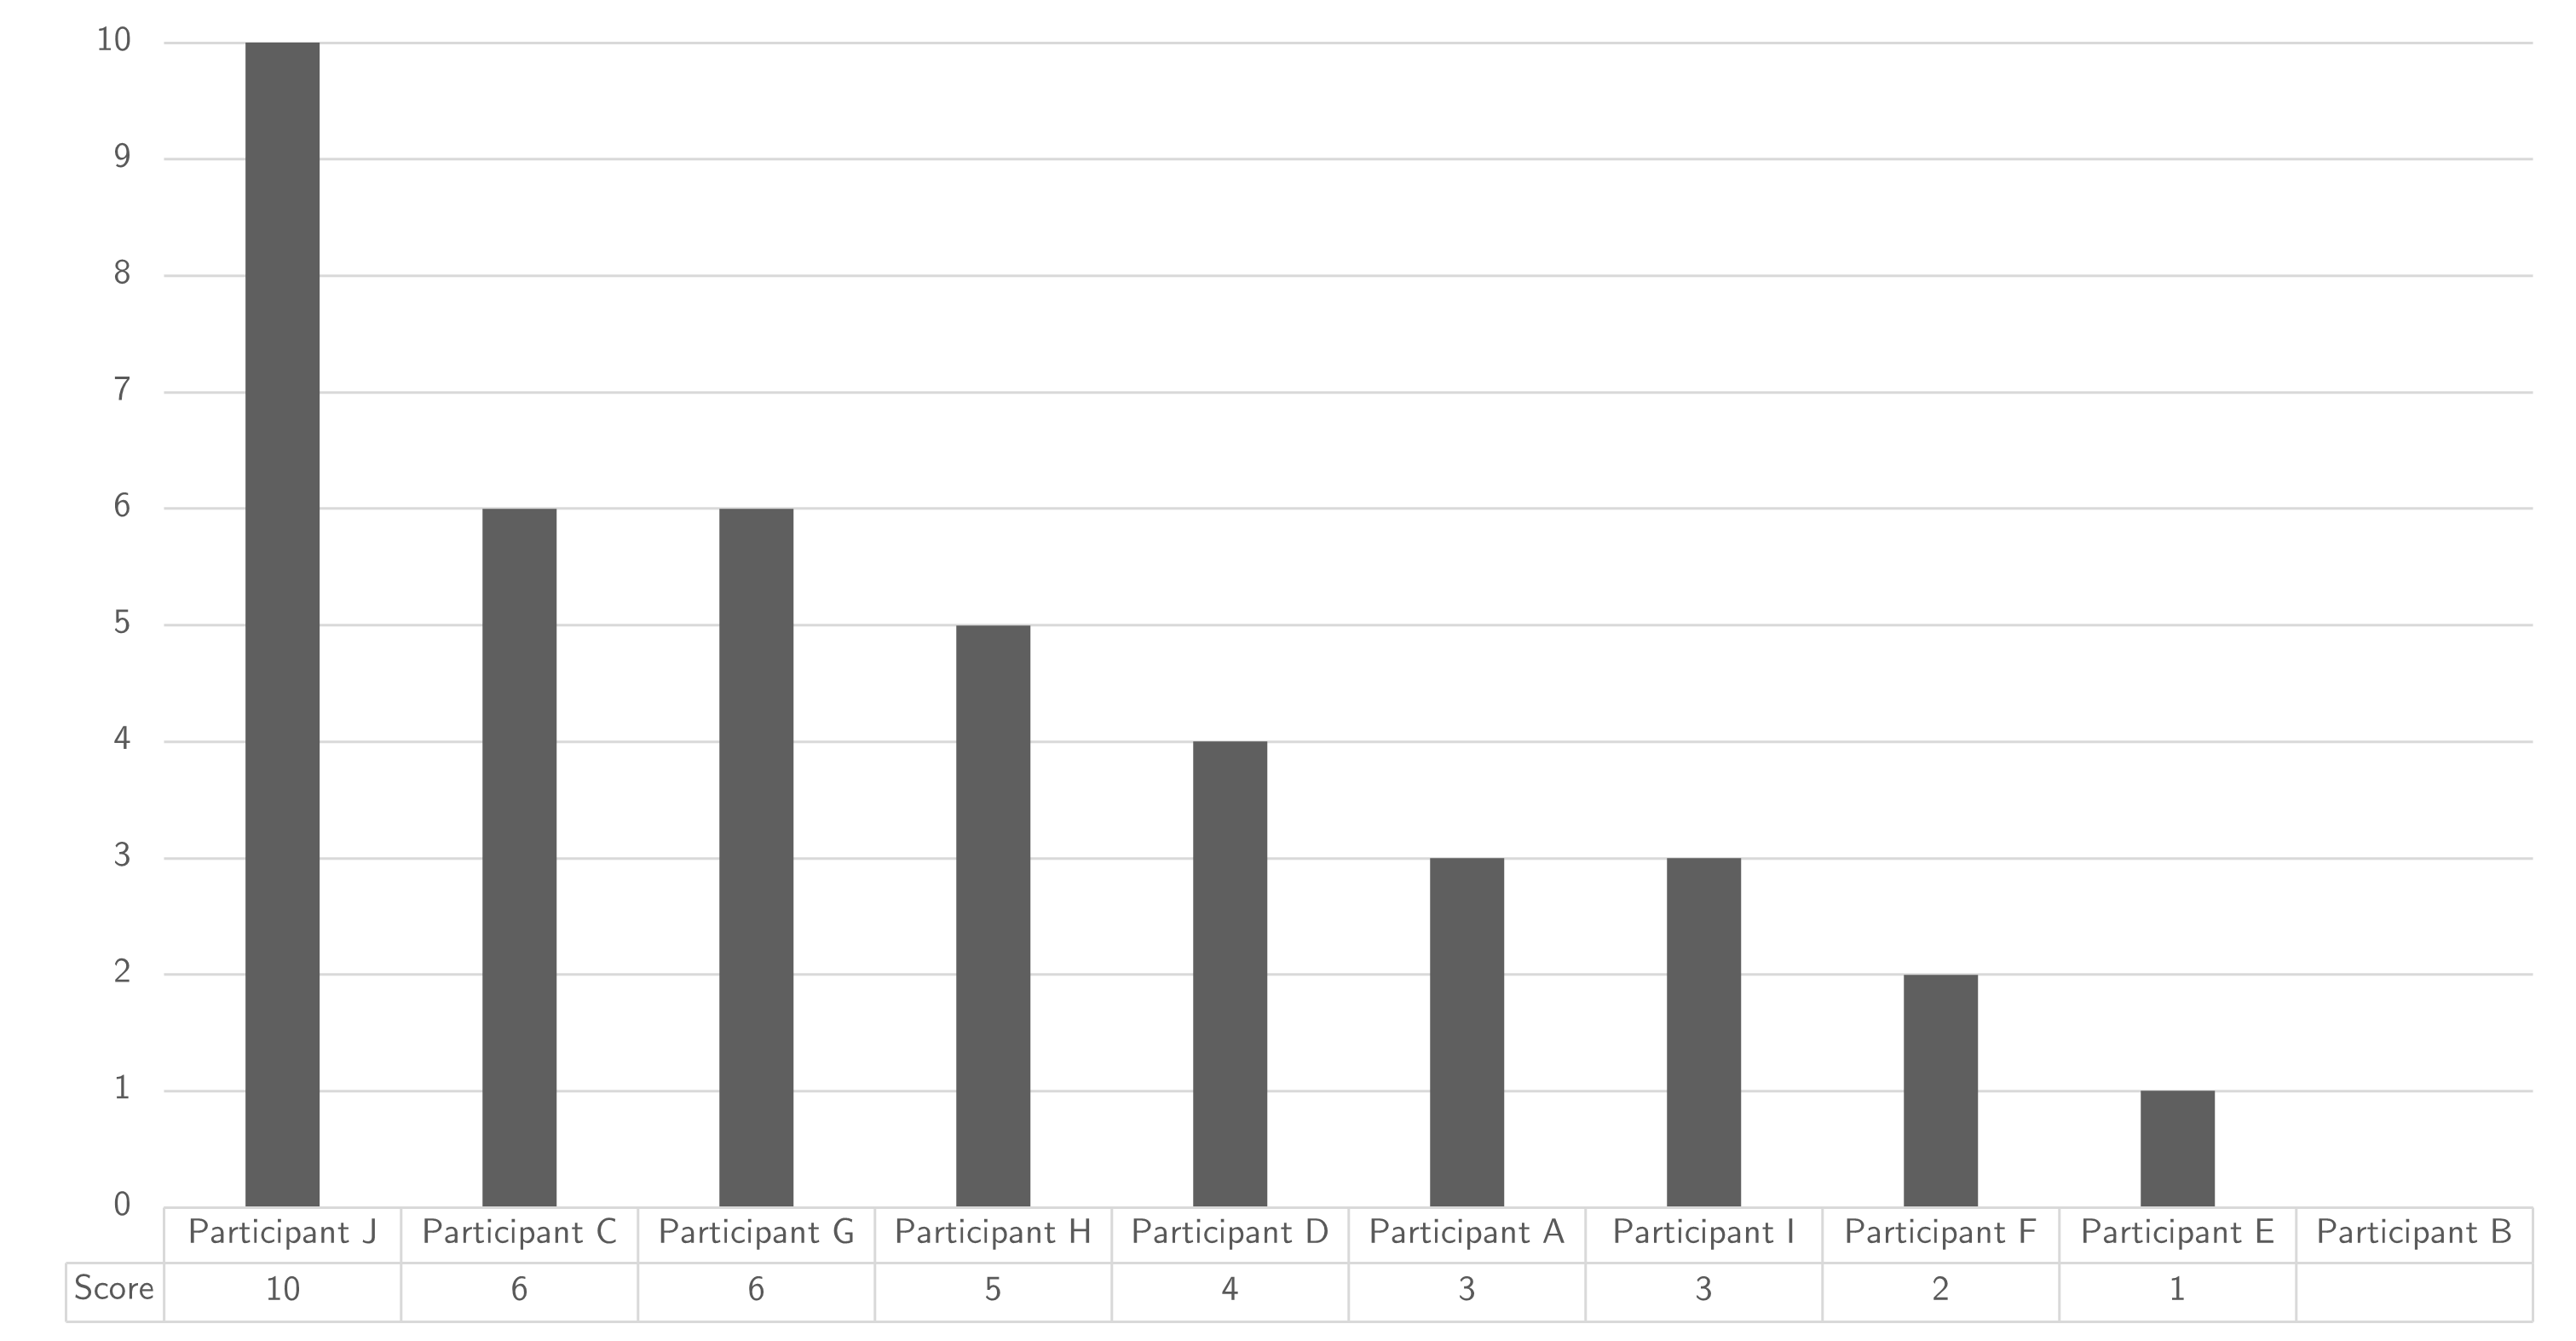
\includegraphics[width=0.9\linewidth]{images/scoreafdatagovernanceplanes}
	\caption[Scoring of antifragile attribute Data Governance Planes]{Scoring of antifragile attribute Data Governance Planes}
	\label{fig:appscoringafdatagovernanceplanes}
\end{figure}
\begin{table}[h!]
	\centering
	\begin{tabular}{ccc}
		\toprule
		\textbf{Rating} & \textbf{Variability} & \textbf{Abstains} \\
		\midrule
		4,4 & 56\% & 1 \\%
		\bottomrule
	\end{tabular}%
	\caption[Scoring of antifragile attribute Data Governance Planes]{Scoring of antifragile attribute Data Governance Planes}
	\label{tab:appscoringafdatagovernance}
\end{table}%
\newpage
\section{Validation of Enterprise Architecture schools of thought}
\begin{table}[!h]
	\centering
	\begin{tabular}{p{.55\textwidth}ccc}
		\toprule
		\textbf{School} & \textbf{Rating} & \textbf{Variability} & \textbf{Abstains} \\
		\midrule
		Enterprise IT Architecting & 5,6 & 34\% & 0 \\%
		Enterprise Integrating & 7,2 & 16\% & 0 \\%
		Enterprise Ecological Adaptation & 8,8 & 27\% & 0 \\%
		\bottomrule
	\end{tabular}%
	\caption{Validation of Enterprise Architecture schools of thought}
	\label{tab:appvalidationofeaschools}%
\end{table}%
\subsection{Enterprise IT Architecting}
\begin{figure}[h!]
	\centering
	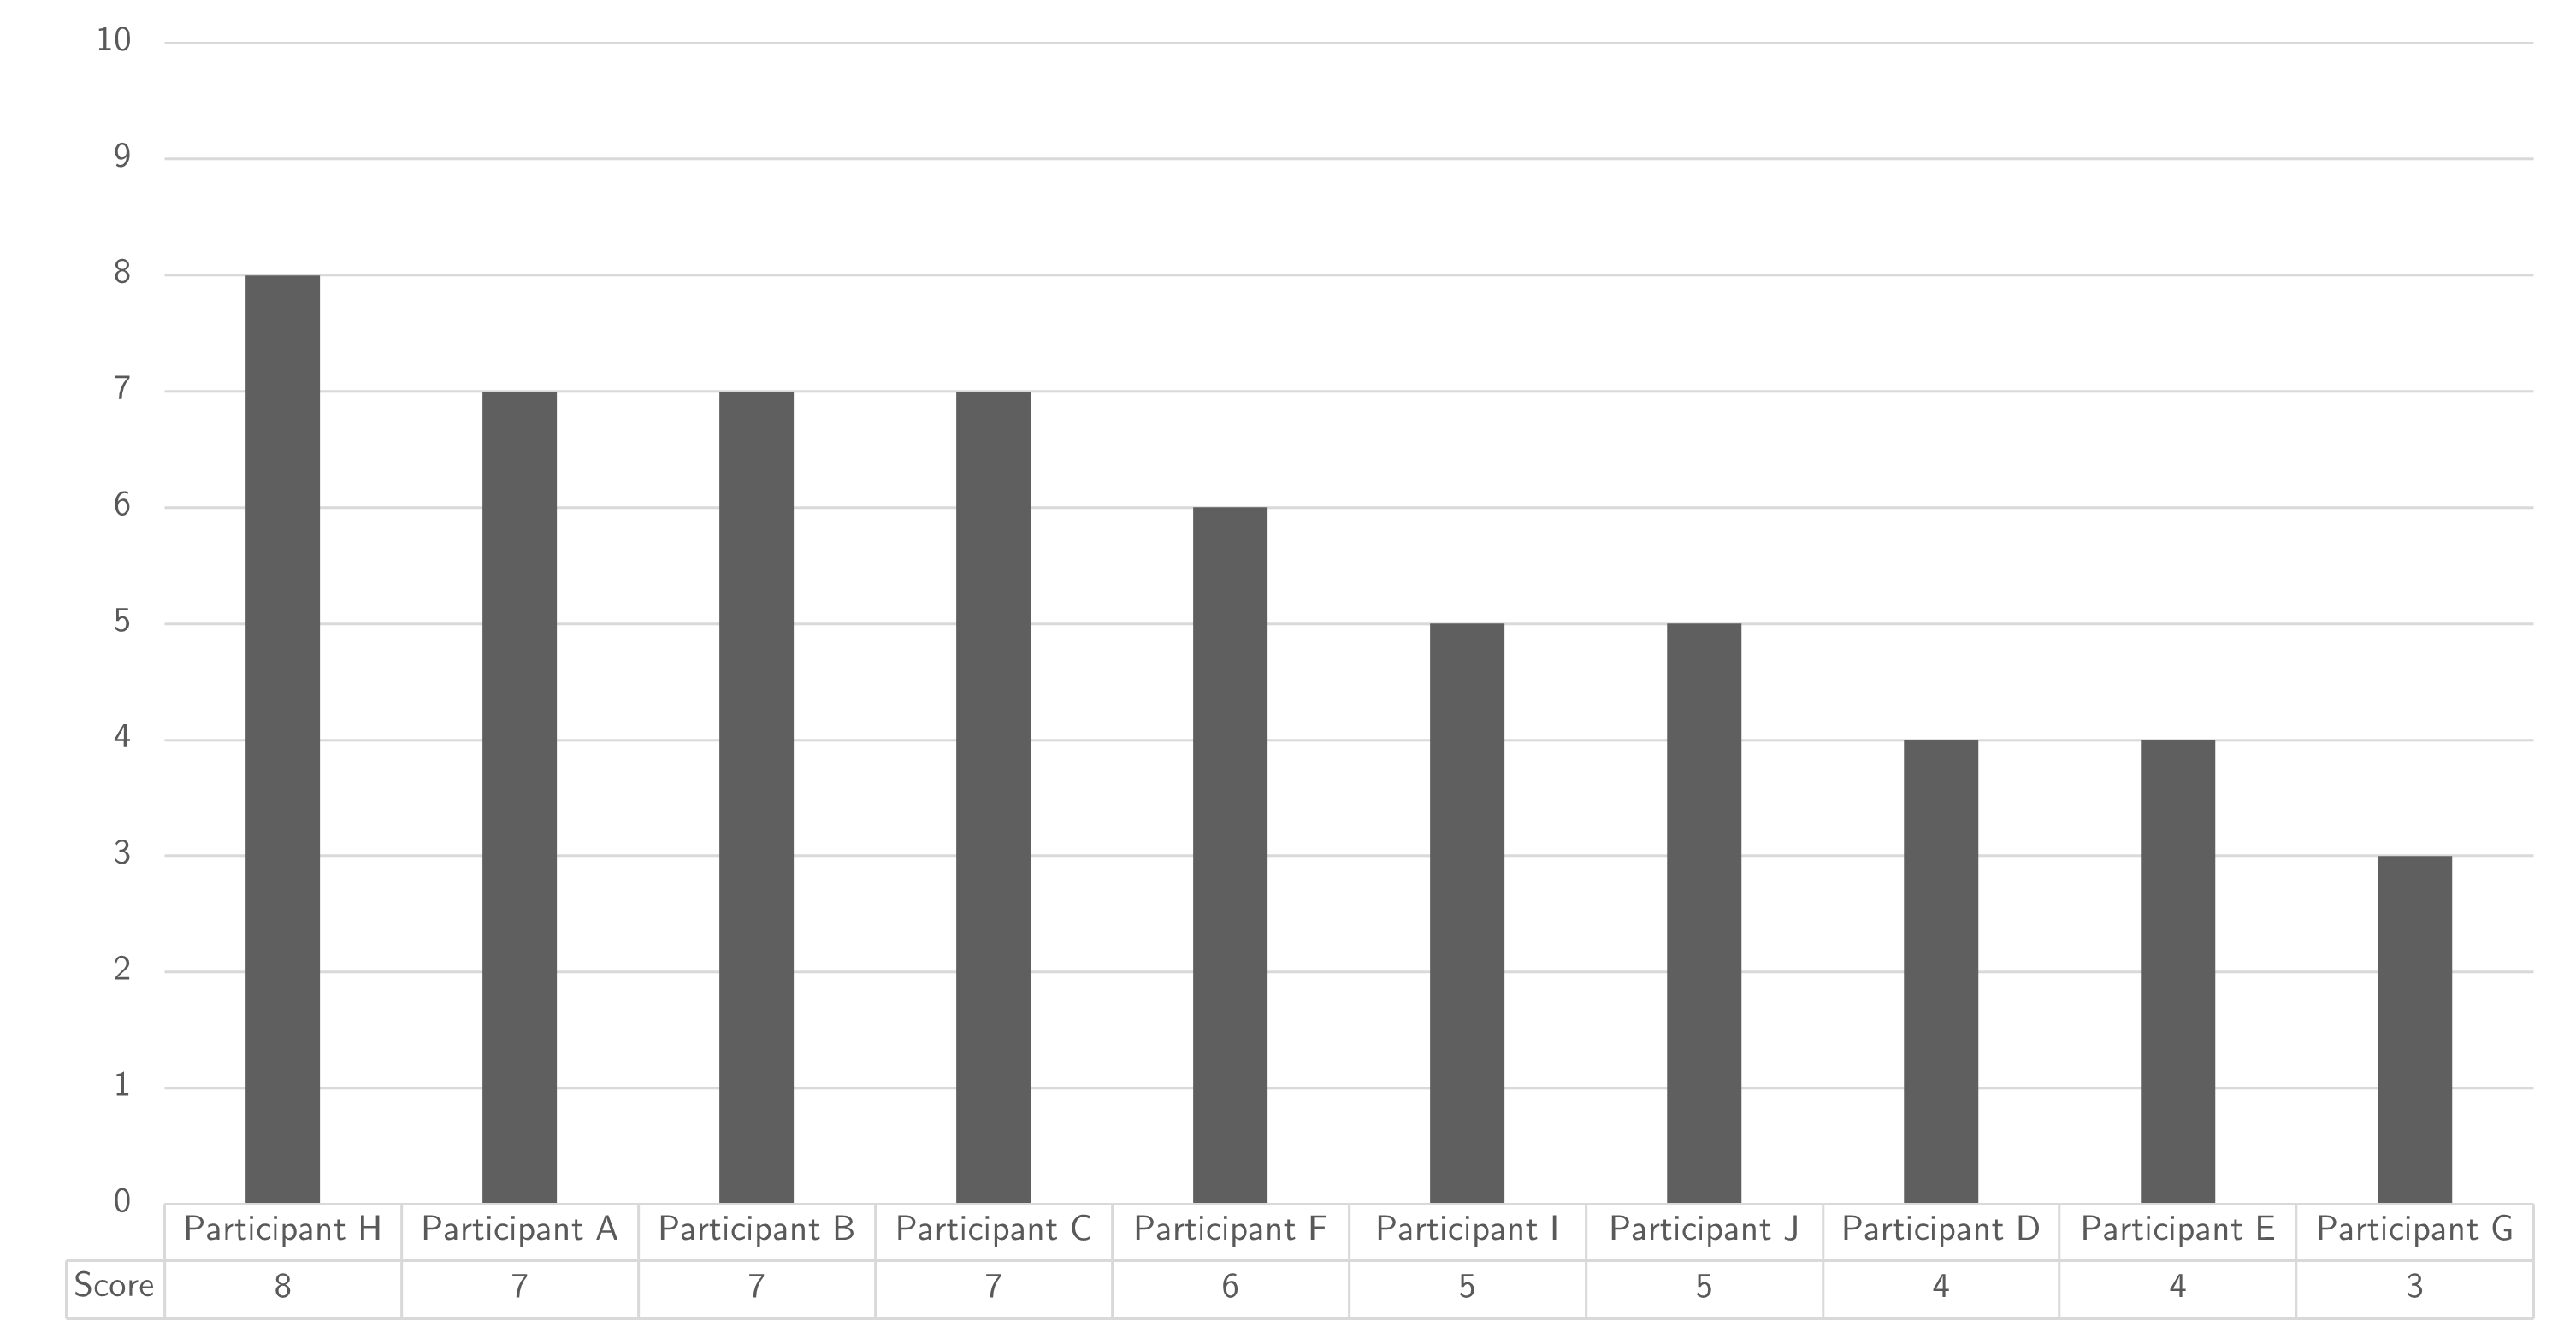
\includegraphics[width=0.9\linewidth]{images/scoreeaschoolenterpriseitarchitecting}
	\caption[Scoring of school of thought Enterprise IT Architecting]{Scoring of school of thought Enterprise IT Architecting}
	\label{fig:appscoringschoolenterpriseitarchitecting}
\end{figure}
\begin{table}[h!]
	\centering
	\begin{tabular}{p{.55\textwidth}ccc}
		\toprule
		\textbf{Attribute} & \textbf{Rating} & \textbf{Variability} & \textbf{Abstains} \\
		\midrule
		Enterprise IT Architecting & 5,6 & 34\% & 0 \\%
		\bottomrule
	\end{tabular}%
	\caption[Scoring of school of thought Enterprise IT Architecting]{Scoring of school of thought Enterprise IT Architecting}
	\label{tab:appscoringschoolenterpriseitarchitecting}%
\end{table}%

\newpage
\subsection{Enterprise Integrating}
\begin{figure}[h!]
	\centering
	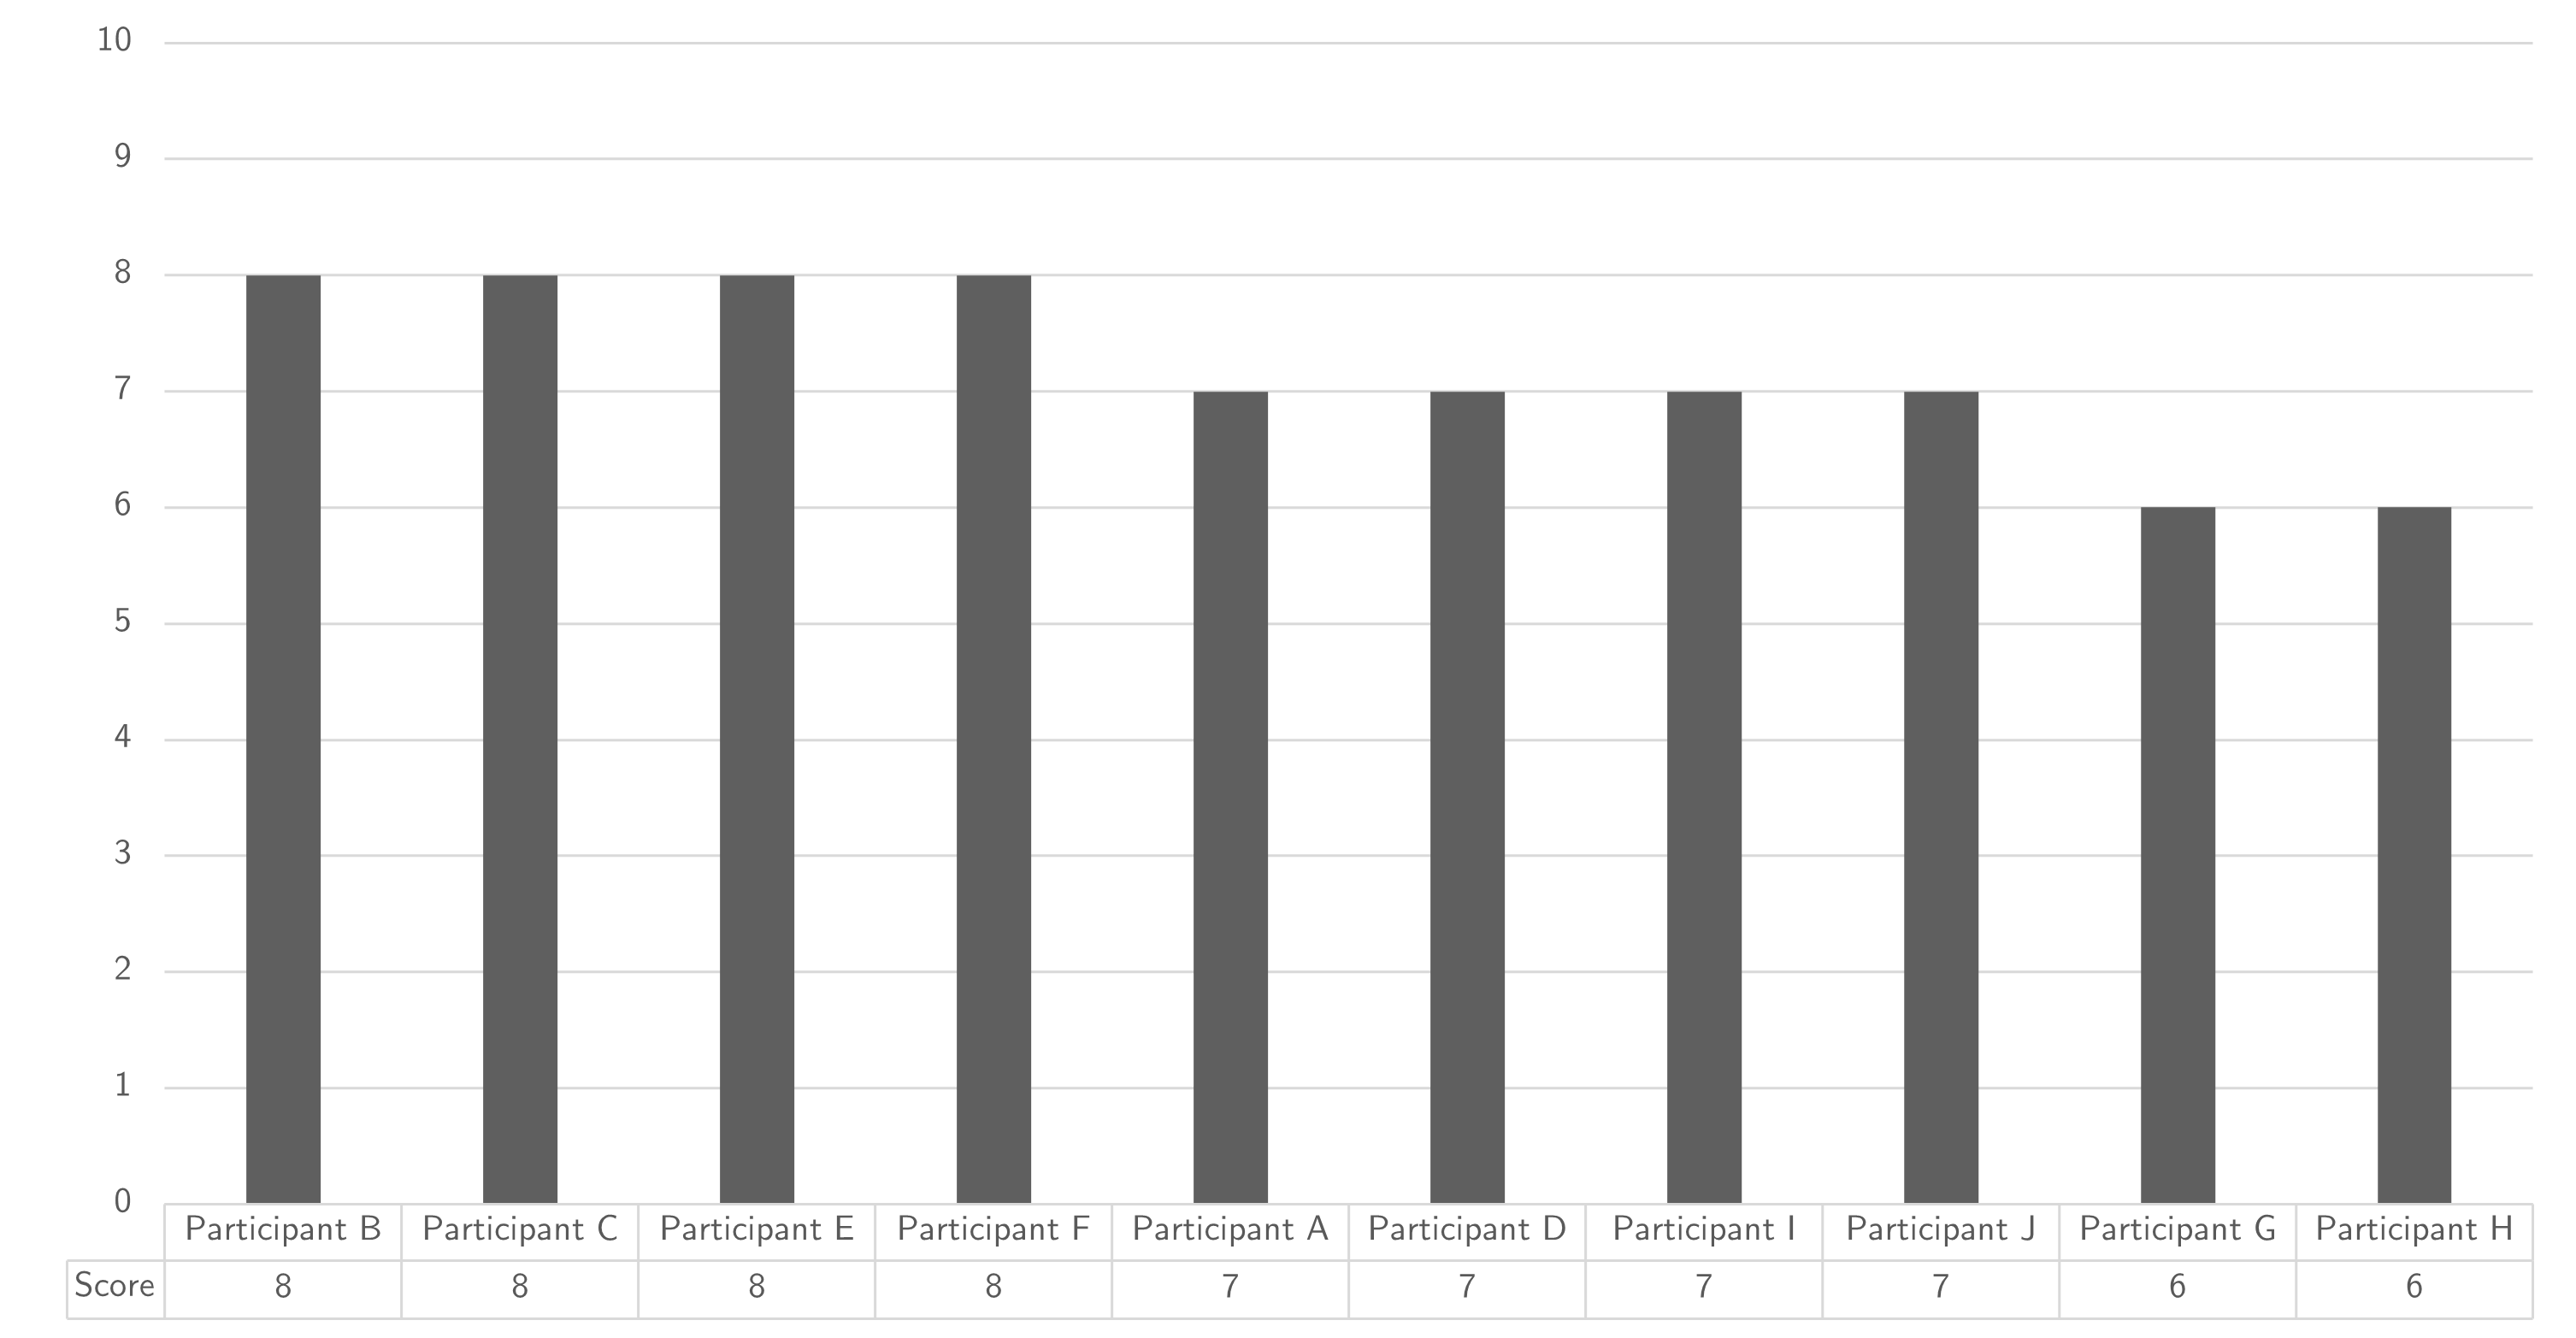
\includegraphics[width=0.9\linewidth]{images/scoreeaschoolenterpriseintegrating}
	\caption[Scoring of school of thought Enterprise Integrating]{Scoring of school of thought Enterprise Integrating}
	\label{fig:appscoringschoolenterpriseintegrating}
\end{figure}
\begin{table}[h!]
	\centering
	\begin{tabular}{p{.55\textwidth}ccc}
		\toprule
		\textbf{Attribute} & \textbf{Rating} & \textbf{Variability} & \textbf{Abstains} \\
		\midrule
		Enterprise Integrating & 7,2 & 16\% & 0 \\%
		\bottomrule
	\end{tabular}%
	\caption[Scoring of school of thought Enterprise Integrating]{Scoring of school of thought Enterprise Integrating}
	\label{tab:appscoringschoolenterpriseintegrating}%
\end{table}%
\newpage
\subsection{Enterprise Ecological Adaptation}
\begin{figure}[h!]
	\centering
	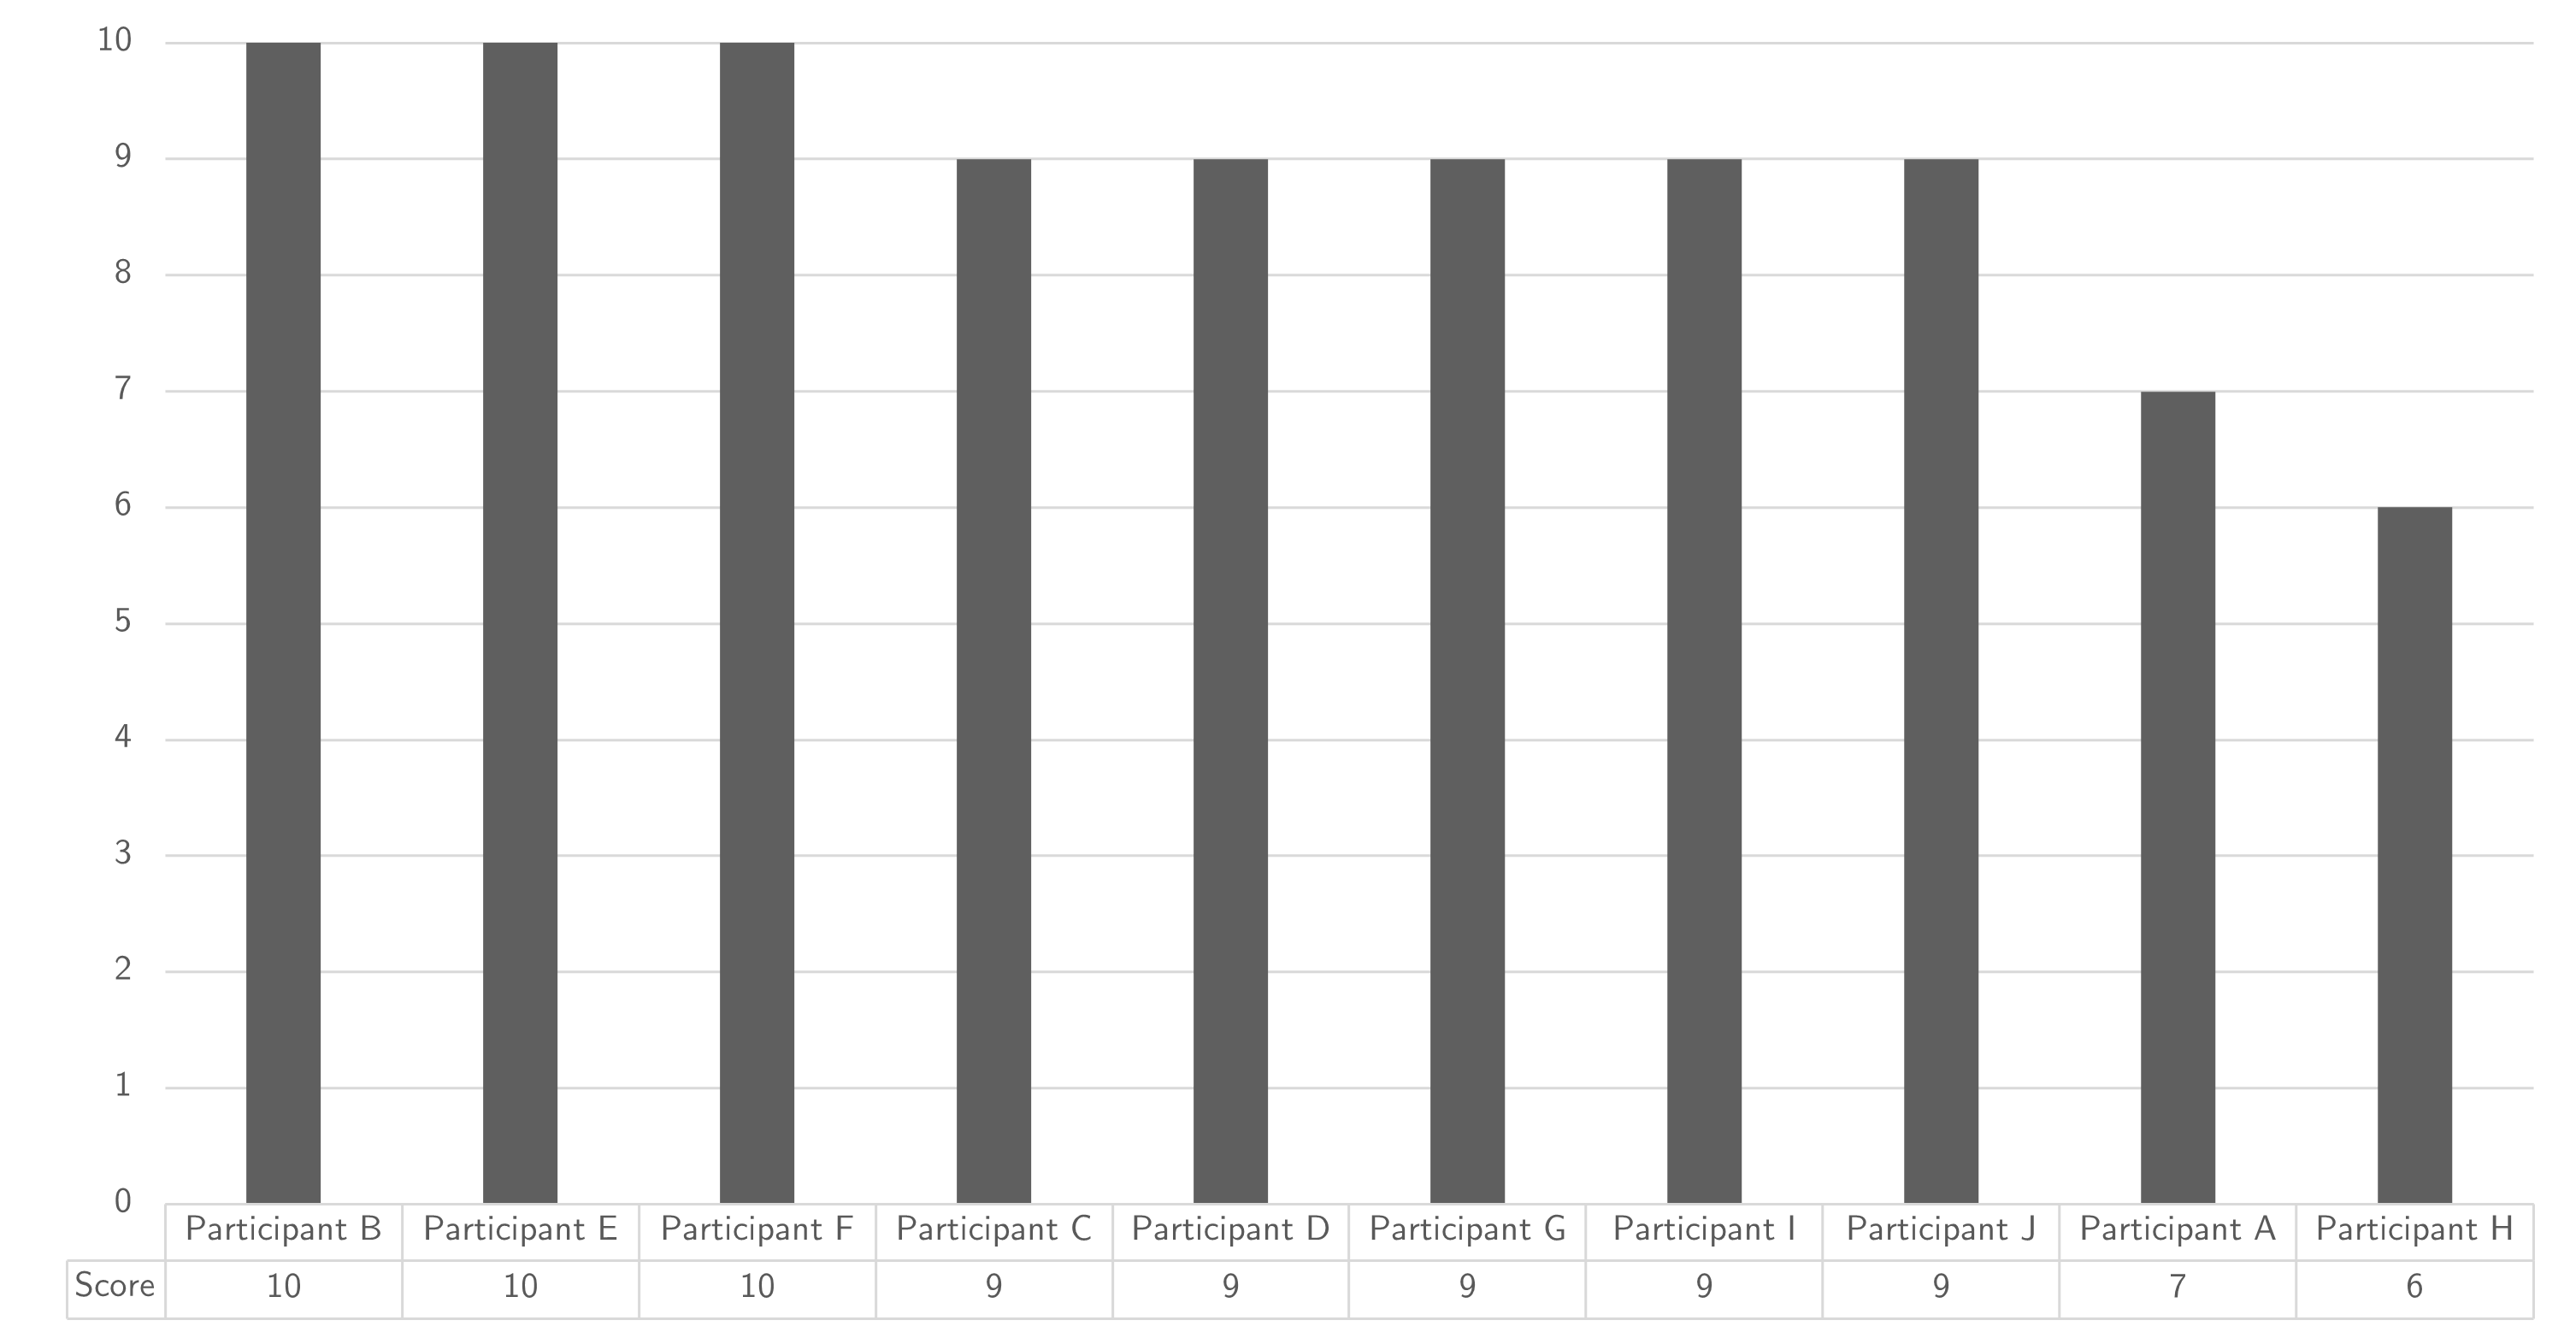
\includegraphics[width=0.9\linewidth]{images/scoreeaschoolenterpriseecologicaladaptation}
	\caption[Scoring of school of thought Enterprise Ecological Adaptation]{Scoring of school of thought Enterprise Ecological Adaptation}
	\label{fig:appscoringschoolenterpriseecologicaladaptation}
\end{figure}
\begin{table}[h!]
	\centering
	\begin{tabular}{p{.55\textwidth}ccc}
		\toprule
		\textbf{Attribute} & \textbf{Rating} & \textbf{Variability} & \textbf{Abstains} \\
		\midrule
		Enterprise Ecological Adaptation & 8,8 & 27\% & 0 \\%
		\bottomrule
	\end{tabular}%
	\caption[Scoring of school of thought Enterprise Ecological Adaptation]{Scoring of school of thought Enterprise Ecological Adaptation}
	\label{tab:appscoringschoolenterpriseecologicaladaptation}%
\end{table}%

\newpage
\section{Validation of Enterprise Architecture attributes}
\begin{table}[!h]
	\centering
	\begin{tabular}{p{.55\textwidth}ccc}
		\toprule
		\textbf{Attribute} & \textbf{Rating} & \textbf{Variability} & \textbf{Abstains} \\
		\midrule
		Systems-in-environment thinking & 7,7 & 28\% & 0 \\%
		Holist (systemic) stance & 7 & 47\% & 0 \\%
		Organisational learning & 7,3 & 44\% & 0 \\%
		Environmental learning & 7,7 & 29\% & 0 \\%
		Intra-organisational coherency & 6,4 & 31\% & 0 \\%
		System-in-environment coevolution learning & 6,6 & 36\% & 0 \\%
		Adapt to business language & 7,1 & 35\% & 0 \\%
		Agile Enterprise & 6,4 & 50\% & 0 \\%
		Real Time Trust (Policy \& Attribute based) & 5,6 & 54\% & 1 \\%
		Foster Dialogue & 6,9 & 32\% & 0 \\%
		Validation & 7,4 & 24\% & 0 \\%
		Altijd goed architectuur & 5,8 & 46\% & 1 \\%
		\bottomrule
	\end{tabular}%
	\caption{Validation of Enterprise Architecture attributes}
	\label{tab:appvalidationofeaattributes}%
\end{table}%
\newpage
\subsection{Systems-in-Environment thinking}
\begin{figure}[h!]
	\centering
	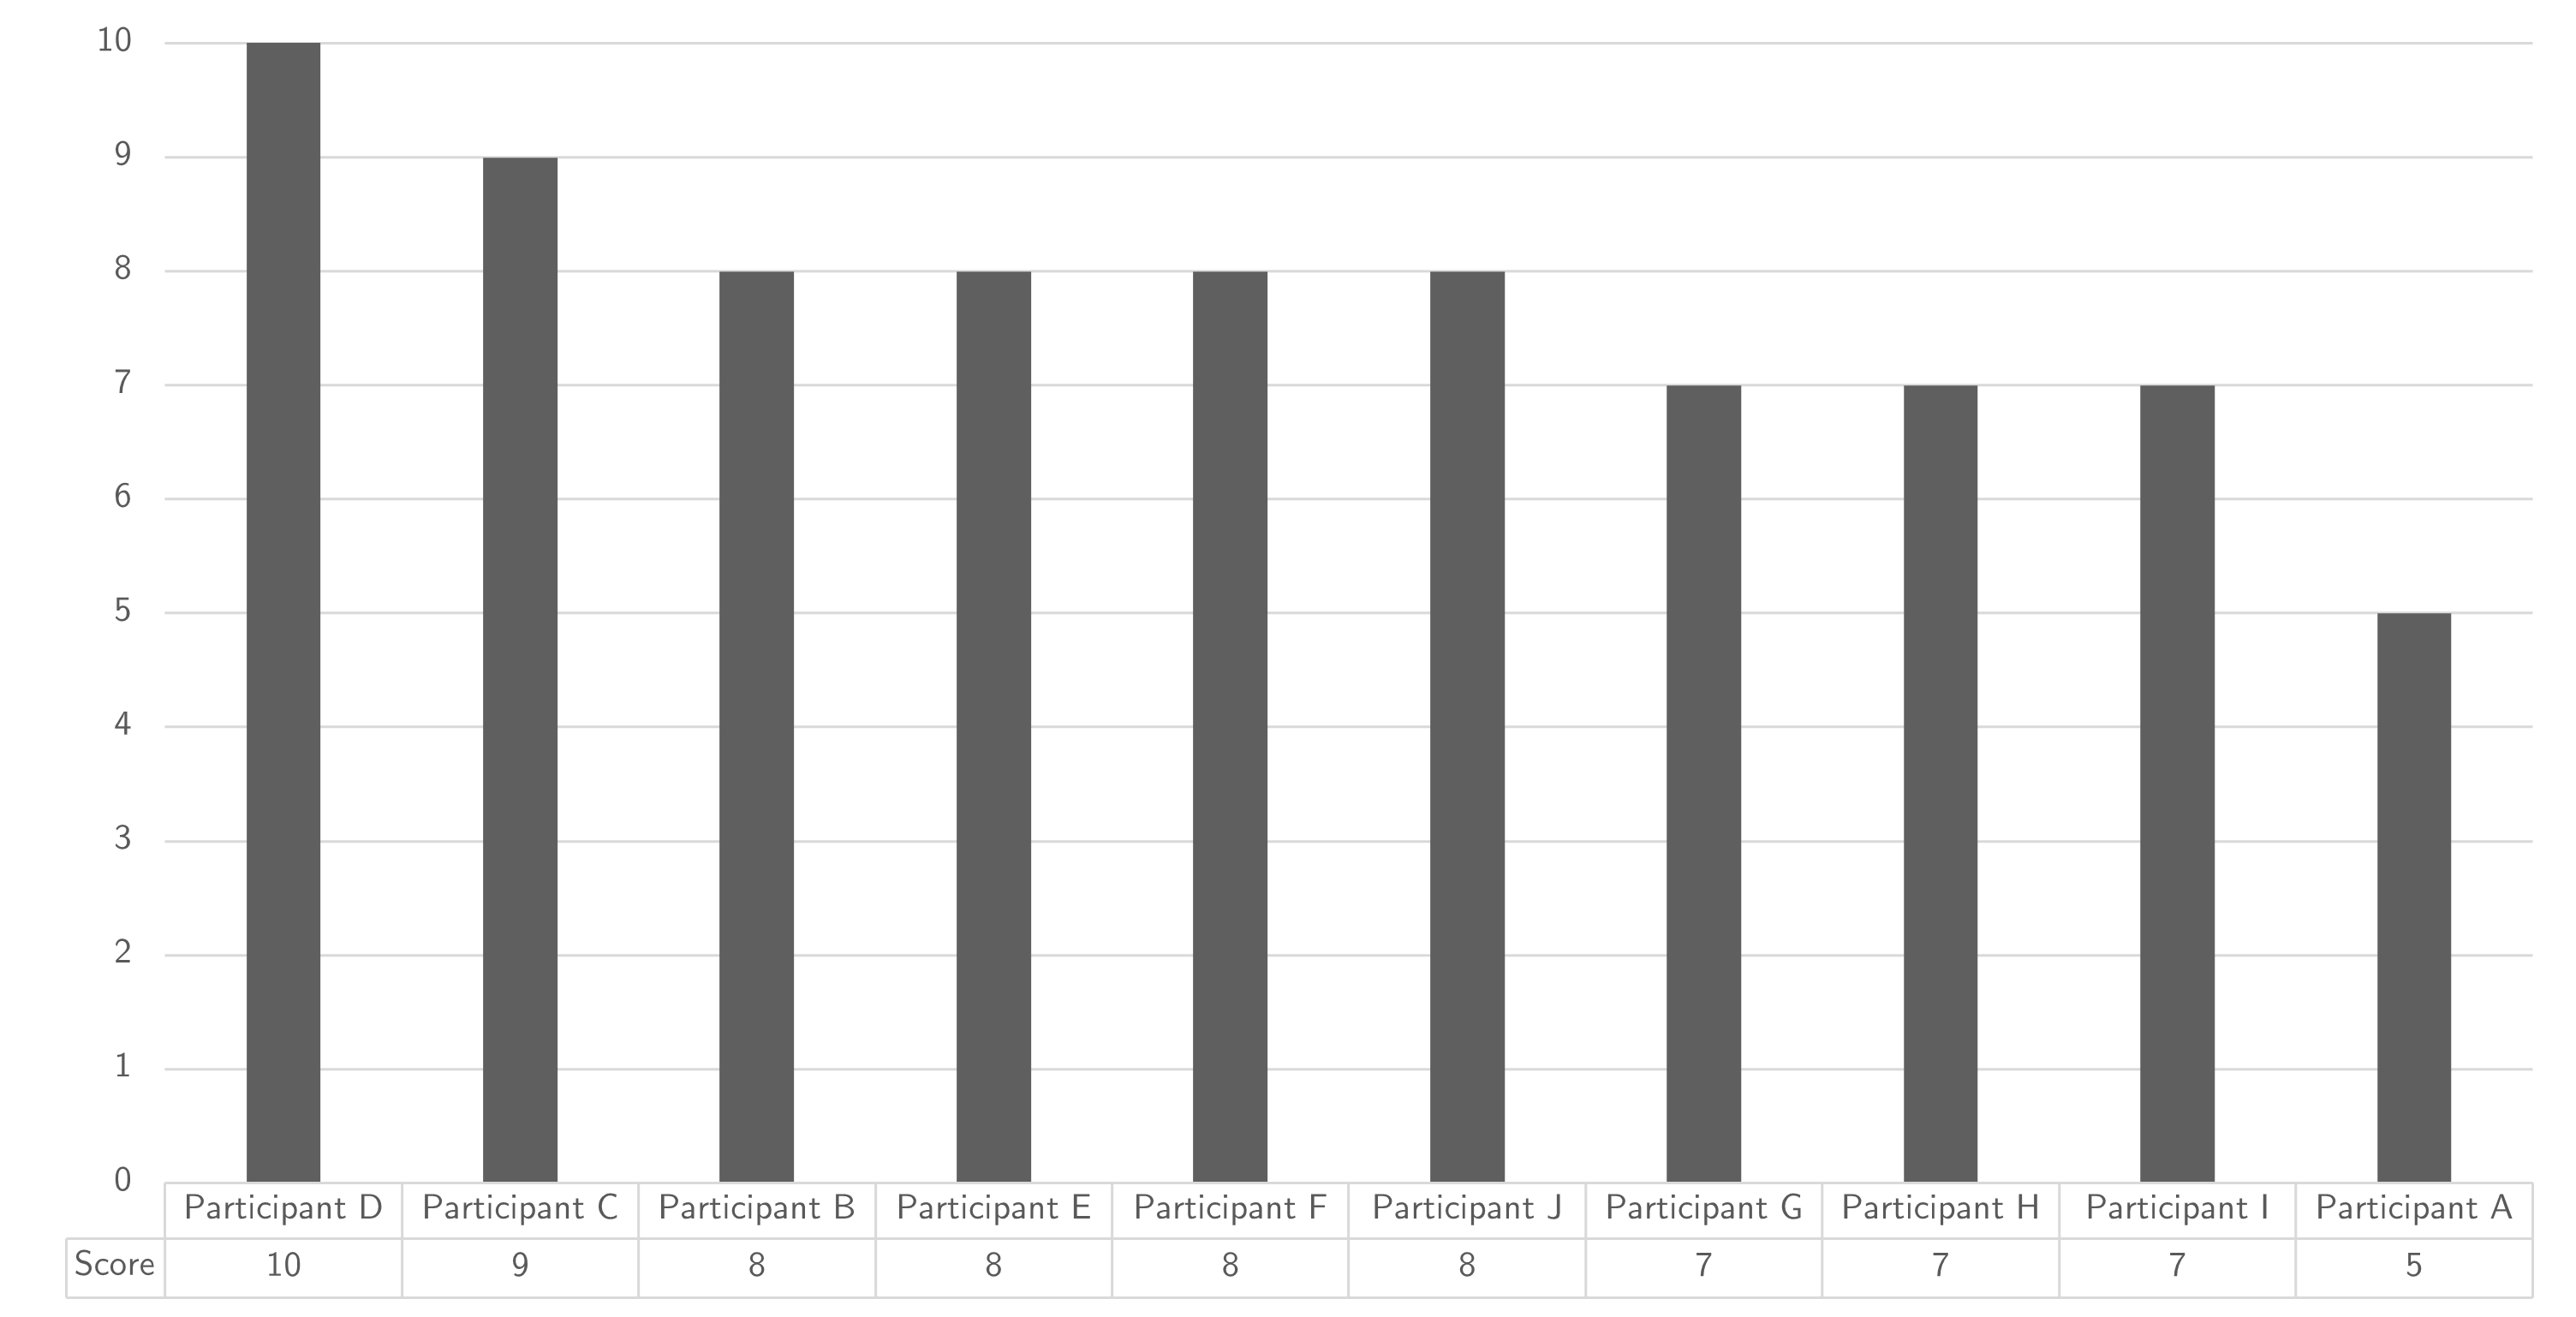
\includegraphics[width=0.9\linewidth]{images/scoreeasystemsinenvironmentthinking}
	\caption[Scoring of EA attribute Systems-in-Environment thinking]{Scoring of EA attribute Systems-in-Environment thinking}
	\label{fig:appscoringeasystemsinenvironmentthinking}
\end{figure}
\begin{table}[h!]
	\centering
	\begin{tabular}{p{.55\textwidth}ccc}
		\toprule
		\textbf{Attribute} & \textbf{Rating} & \textbf{Variability} & \textbf{Abstains} \\
		\midrule
		Systems-in-environment thinking & 7,7 & 28\% & 0 \\%
		\bottomrule
	\end{tabular}%
	\caption[Scoring of EA attribute Systems-in-Environment thinking]{Scoring of EA attribute Systems-in-Environment thinking}
	\label{tab:appscoringeasystemsinenvironmentthinking}%
\end{table}%
\newpage
\subsection{Holistic (systemic) stance}
\begin{figure}[h!]
	\centering
	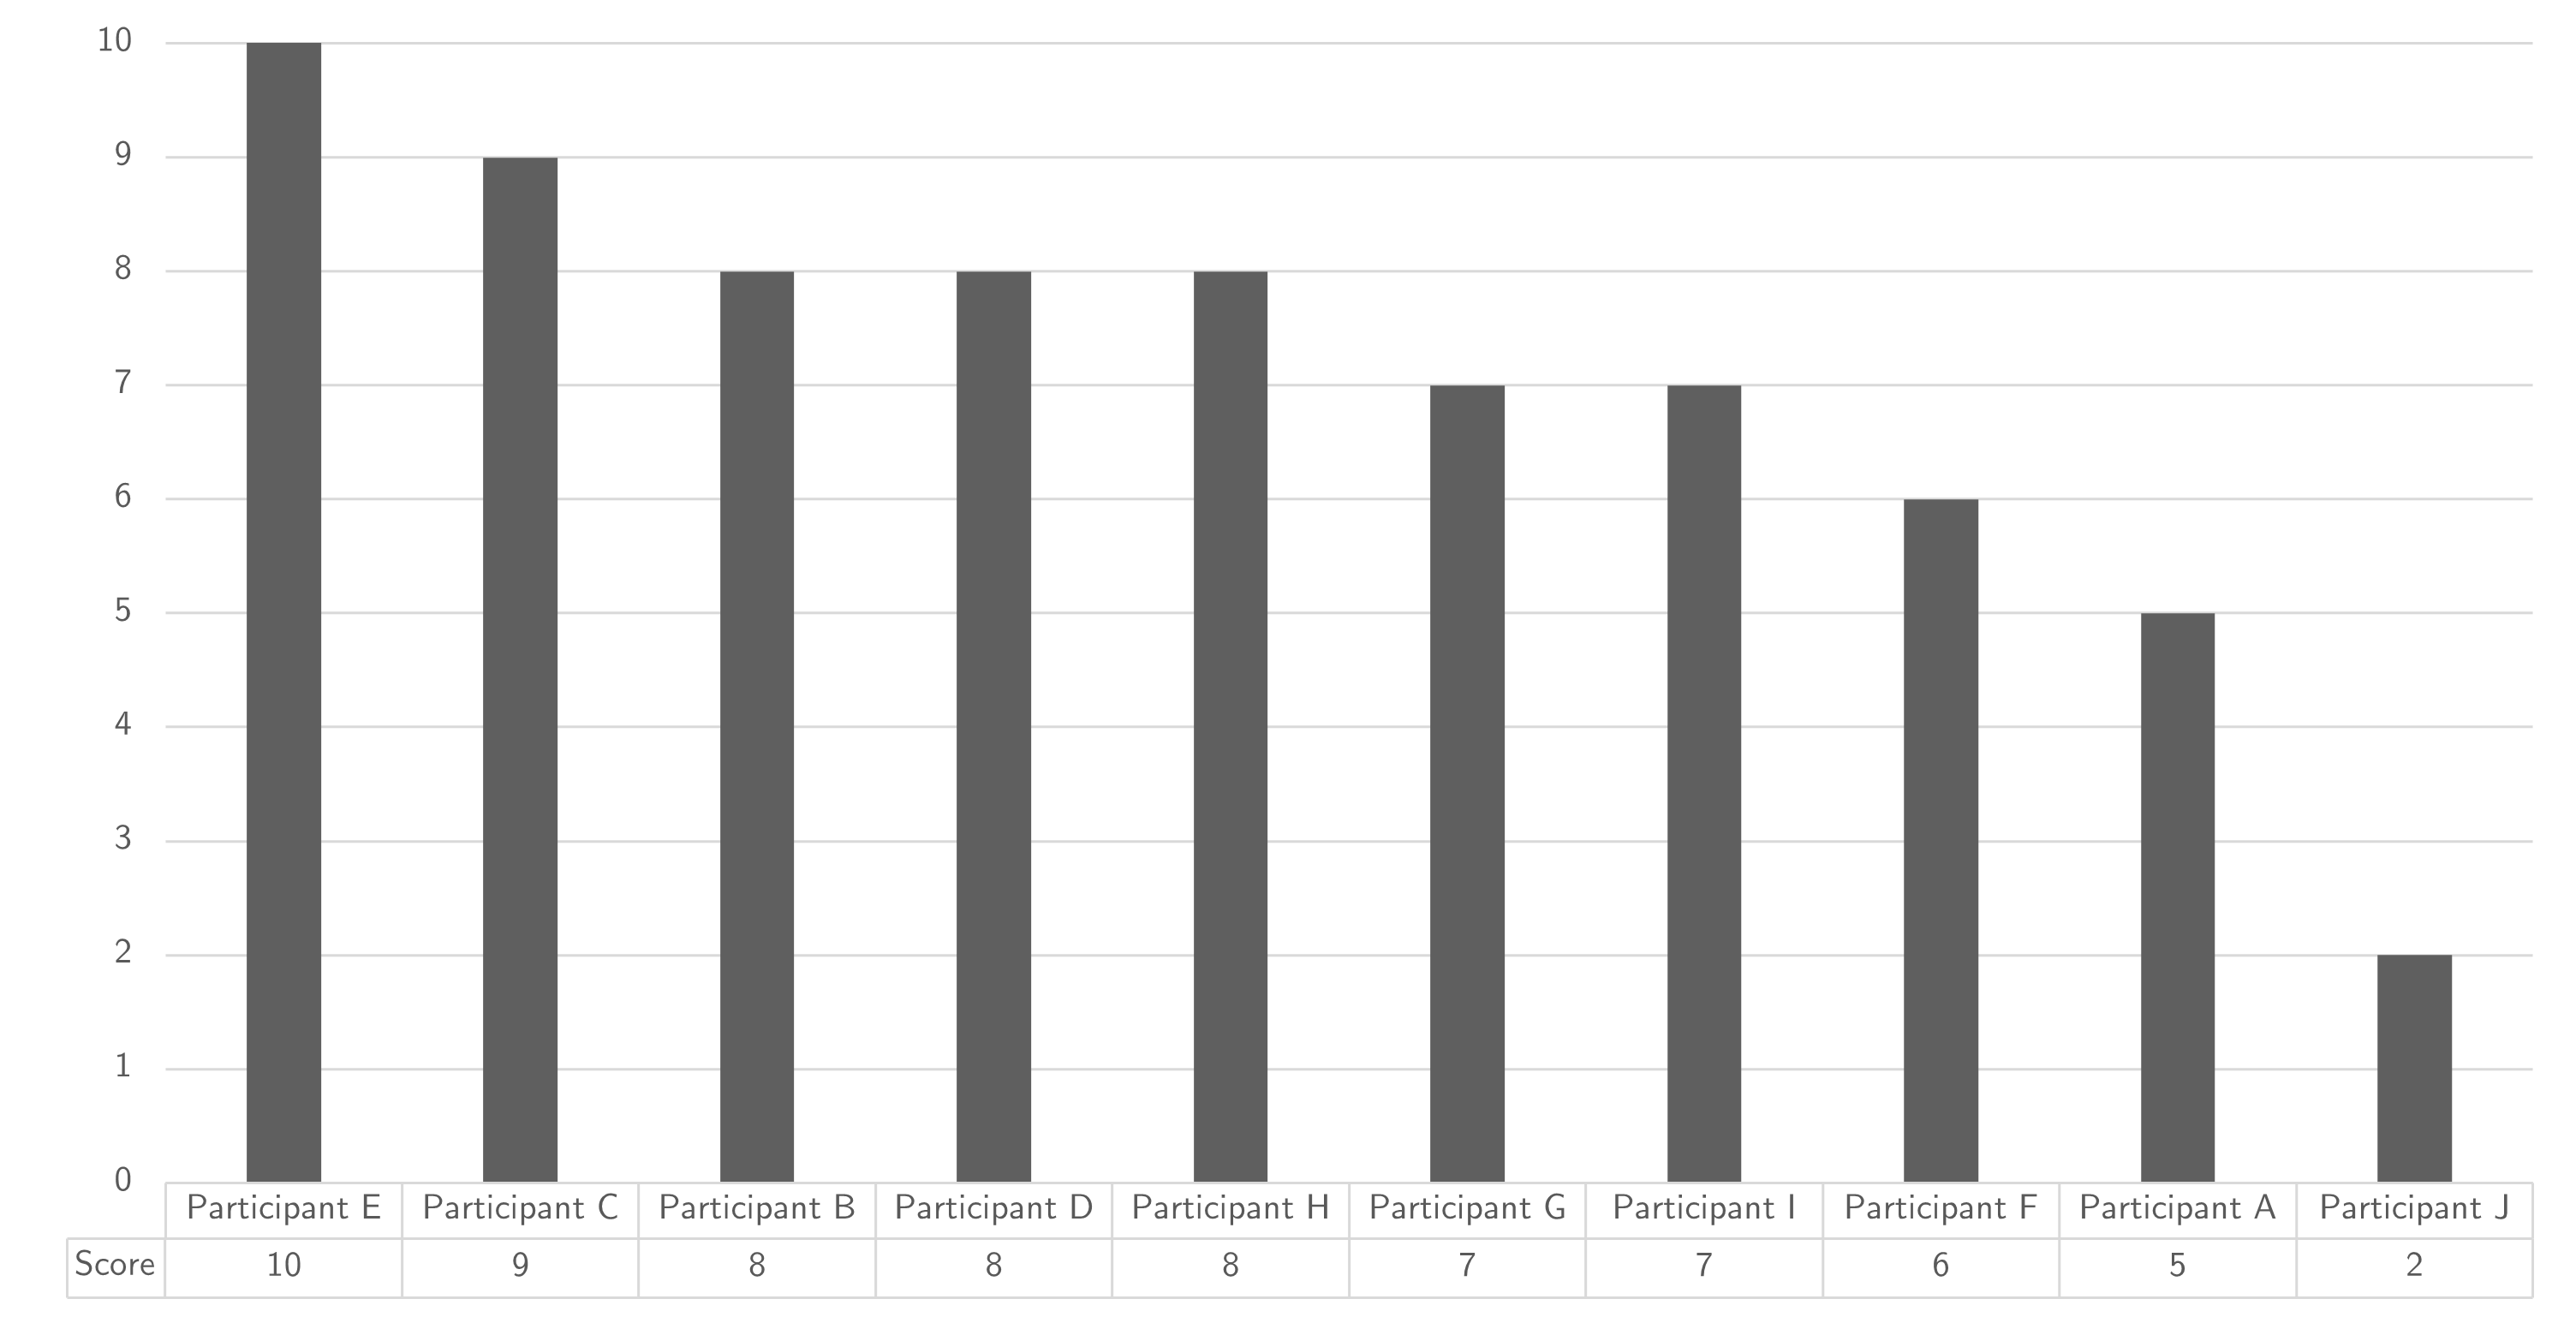
\includegraphics[width=0.9\linewidth]{images/scoreeaholisticsystemsstance}
	\caption[Scoring of EA attribute Holistic (systemic) stance]{Scoring of EA attribute Holistic (systemic) stance}
	\label{fig:appscoringeaholisticsystemsstance}
\end{figure}
\begin{table}[h!]
	\centering
	\begin{tabular}{p{.55\textwidth}ccc}
		\toprule
		\textbf{Attribute} & \textbf{Rating} & \textbf{Variability} & \textbf{Abstains} \\
		\midrule
		Holist (systemic) stance & 7 & 47\% & 0 \\%
		\bottomrule
	\end{tabular}%
	\caption[Scoring of EA attribute Holistic (systemic) stance]{Scoring of EA attribute Holistic (systemic) stance}
	\label{tab:appscoringeaholisticsystemsstance}%
\end{table}%
\newpage
\subsection{Organisational learning}
\begin{figure}[h!]
	\centering
	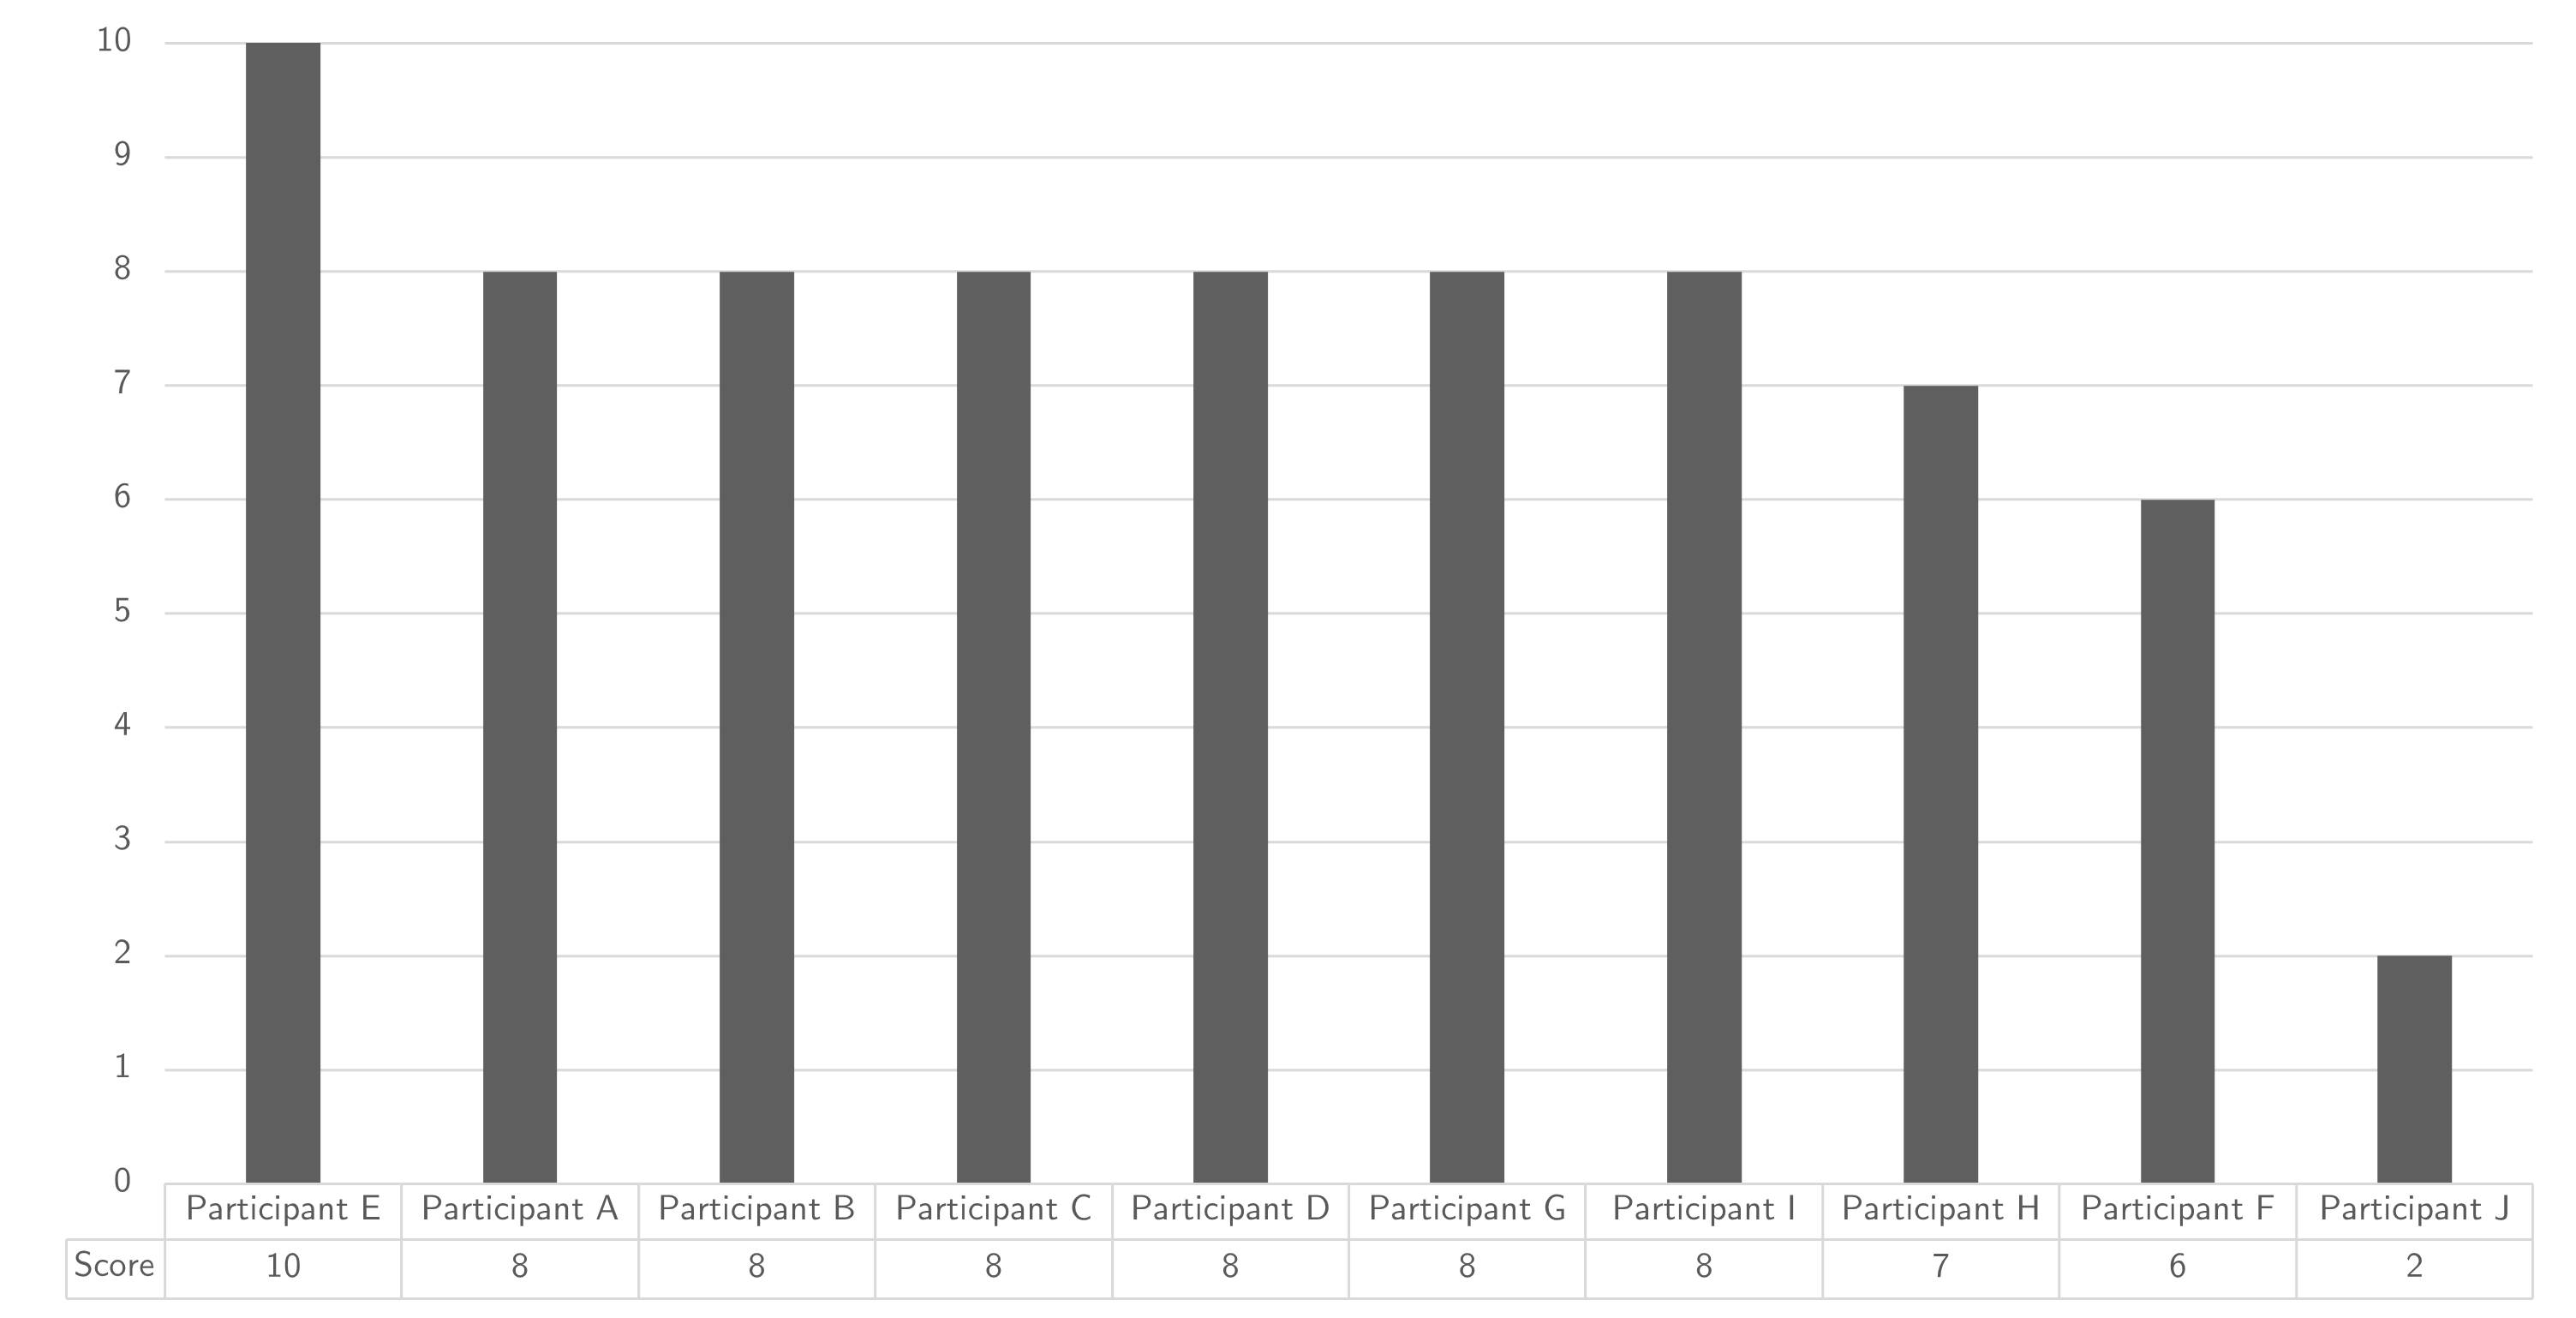
\includegraphics[width=0.9\linewidth]{images/scoreeaorganisationallearning}
	\caption[Scoring of EA attribute Organisational learning]{Scoring of EA attribute Organisational learning}
	\label{fig:appscoringeaorganiationallearning}
\end{figure}
\begin{table}[h!]
	\centering
	\begin{tabular}{p{.55\textwidth}ccc}
		\toprule
		\textbf{Attribute} & \textbf{Rating} & \textbf{Variability} & \textbf{Abstains} \\
		\midrule
		Organisational learning & 7,3 & 44\% & 0 \\%
		\bottomrule
	\end{tabular}%
	\caption[Scoring of EA attribute Organisational learning]{Scoring of EA attribute Organisational learning}
	\label{tab:appscoringeaorganisationallearning}%
\end{table}%
\newpage
\subsection{Environmental learning}
\begin{figure}[h!]
	\centering
	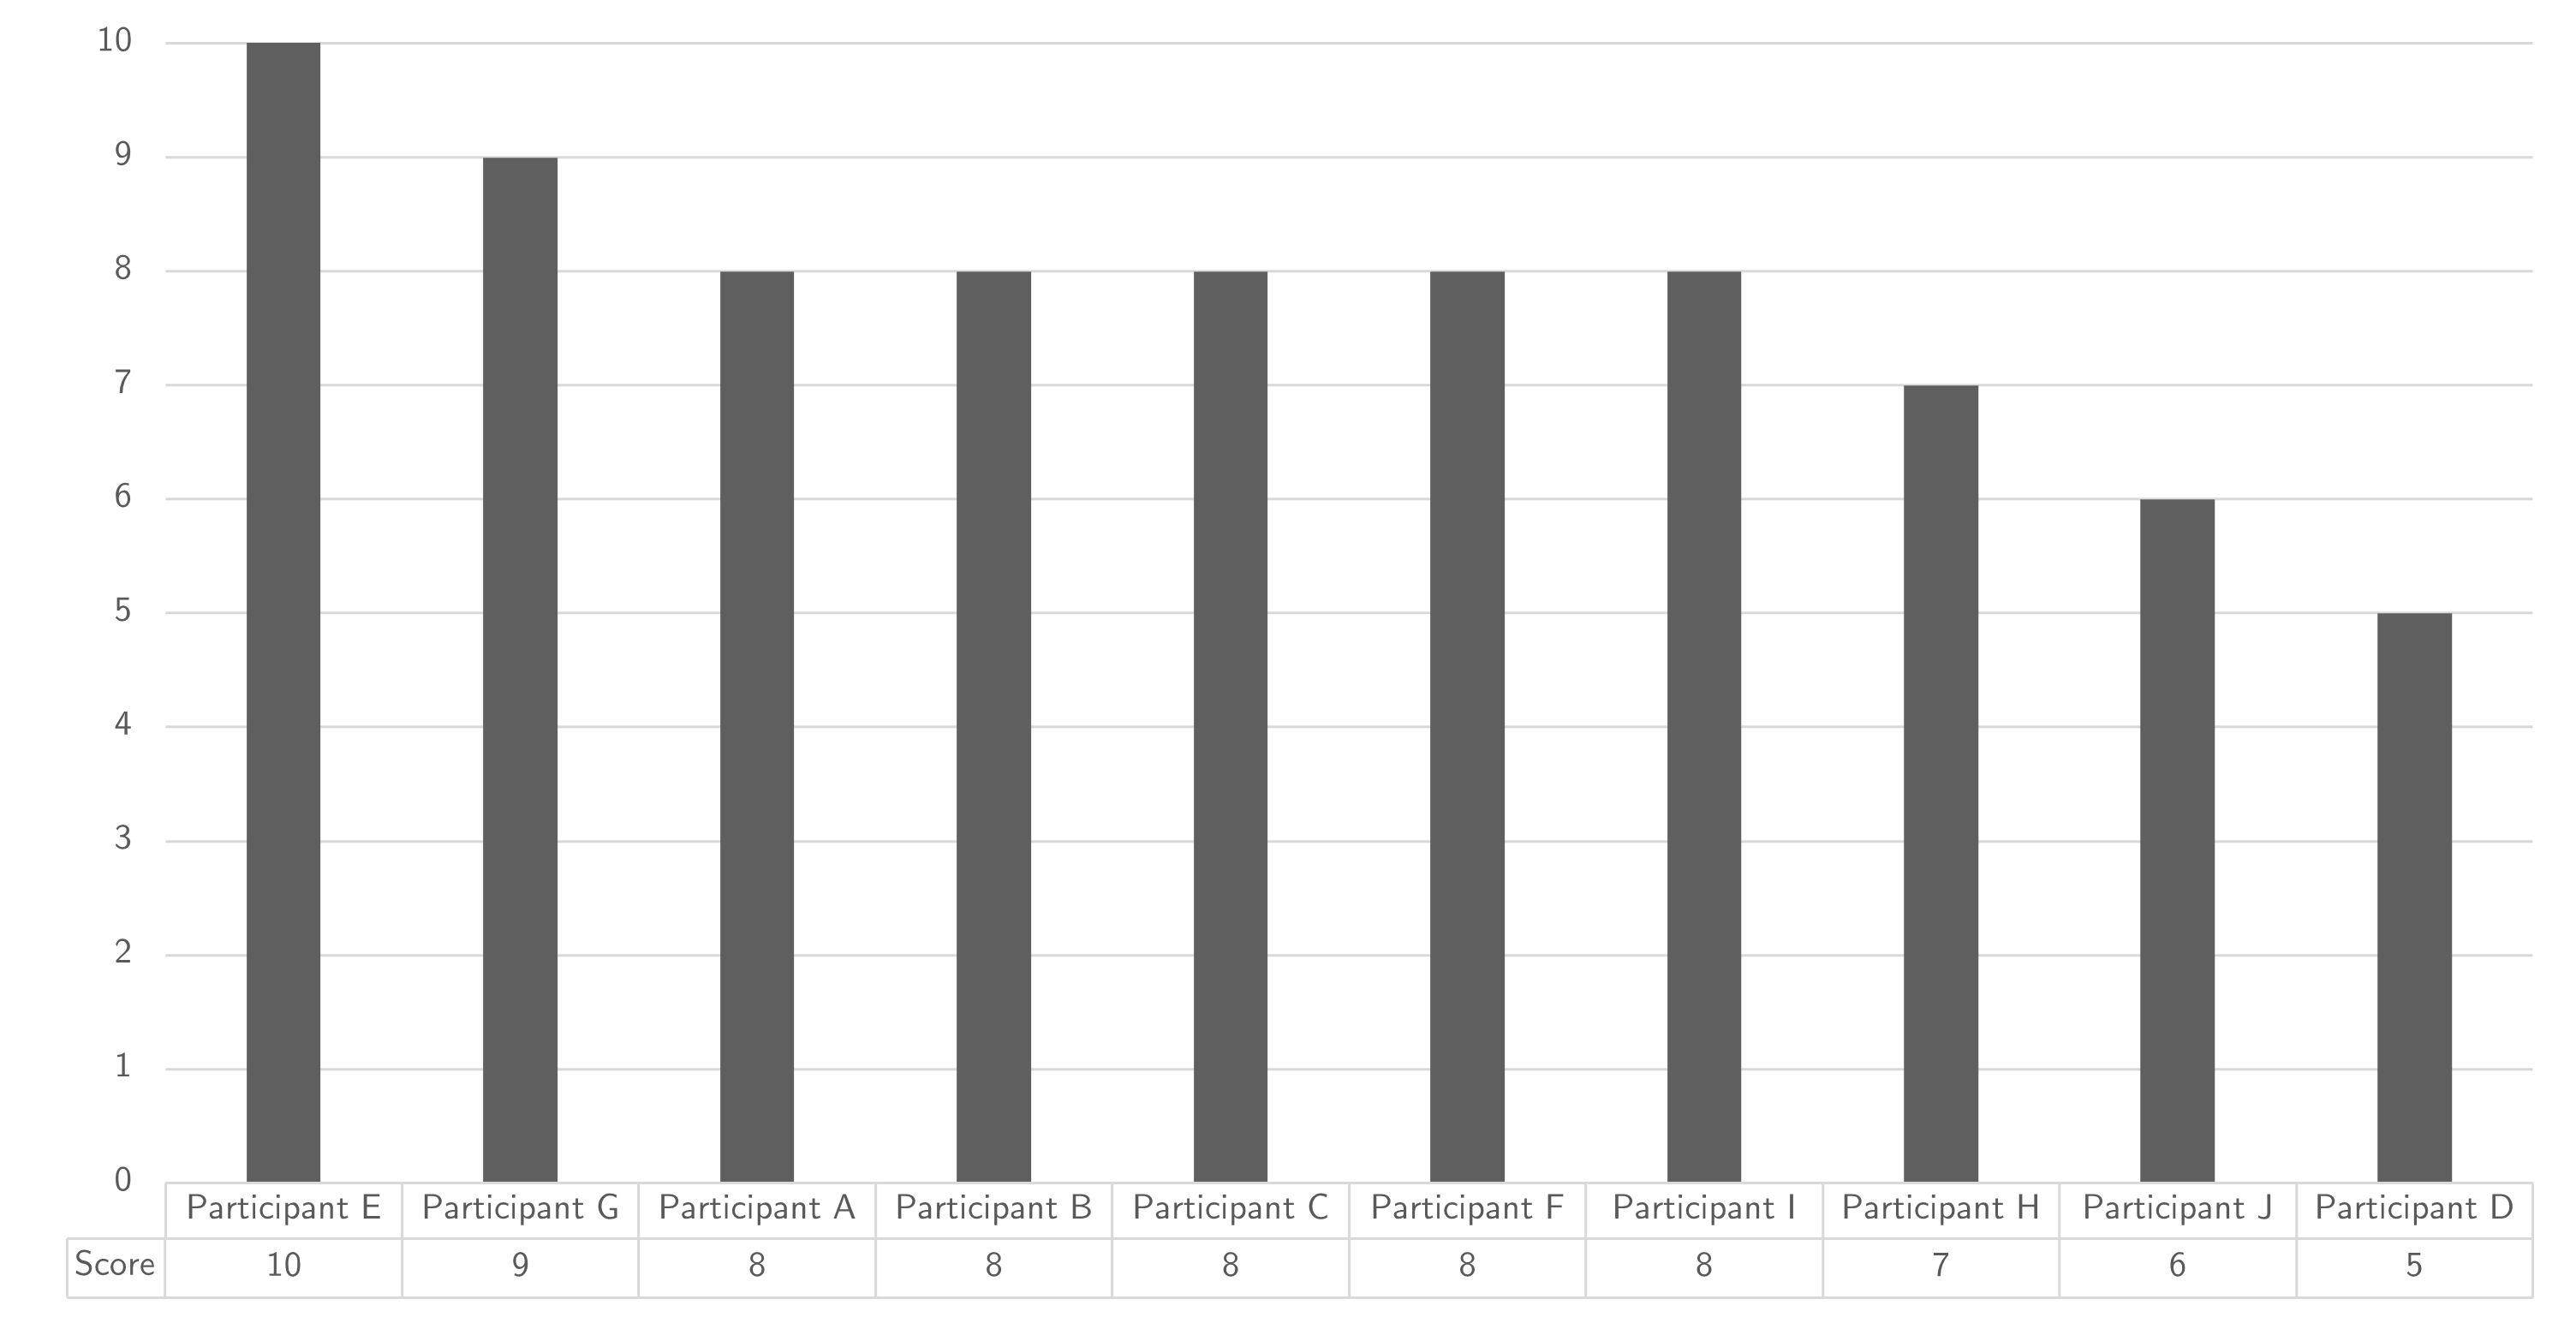
\includegraphics[width=0.9\linewidth]{images/scoreeaenvironmentallearning}
	\caption[Scoring of EA attribute Environmental learning]{Scoring of EA attribute Environmental learning}
	\label{fig:appscoringeaenvironmentallearning}
\end{figure}
\begin{table}[h!]
	\centering
	\begin{tabular}{p{.55\textwidth}ccc}
		\toprule
		\textbf{Attribute} & \textbf{Rating} & \textbf{Variability} & \textbf{Abstains} \\
		\midrule
		Environmental learning & 7,7 & 29\% & 0 \\%
		\bottomrule
	\end{tabular}%
	\caption[Scoring of EA attribute Environmental learning]{Scoring of EA attribute Environmental learning}
	\label{tab:appscoringeaenvironmentallearning}%
\end{table}%
\newpage
\subsection{Intra-organisational coherency}
\begin{figure}[h!]
	\centering
	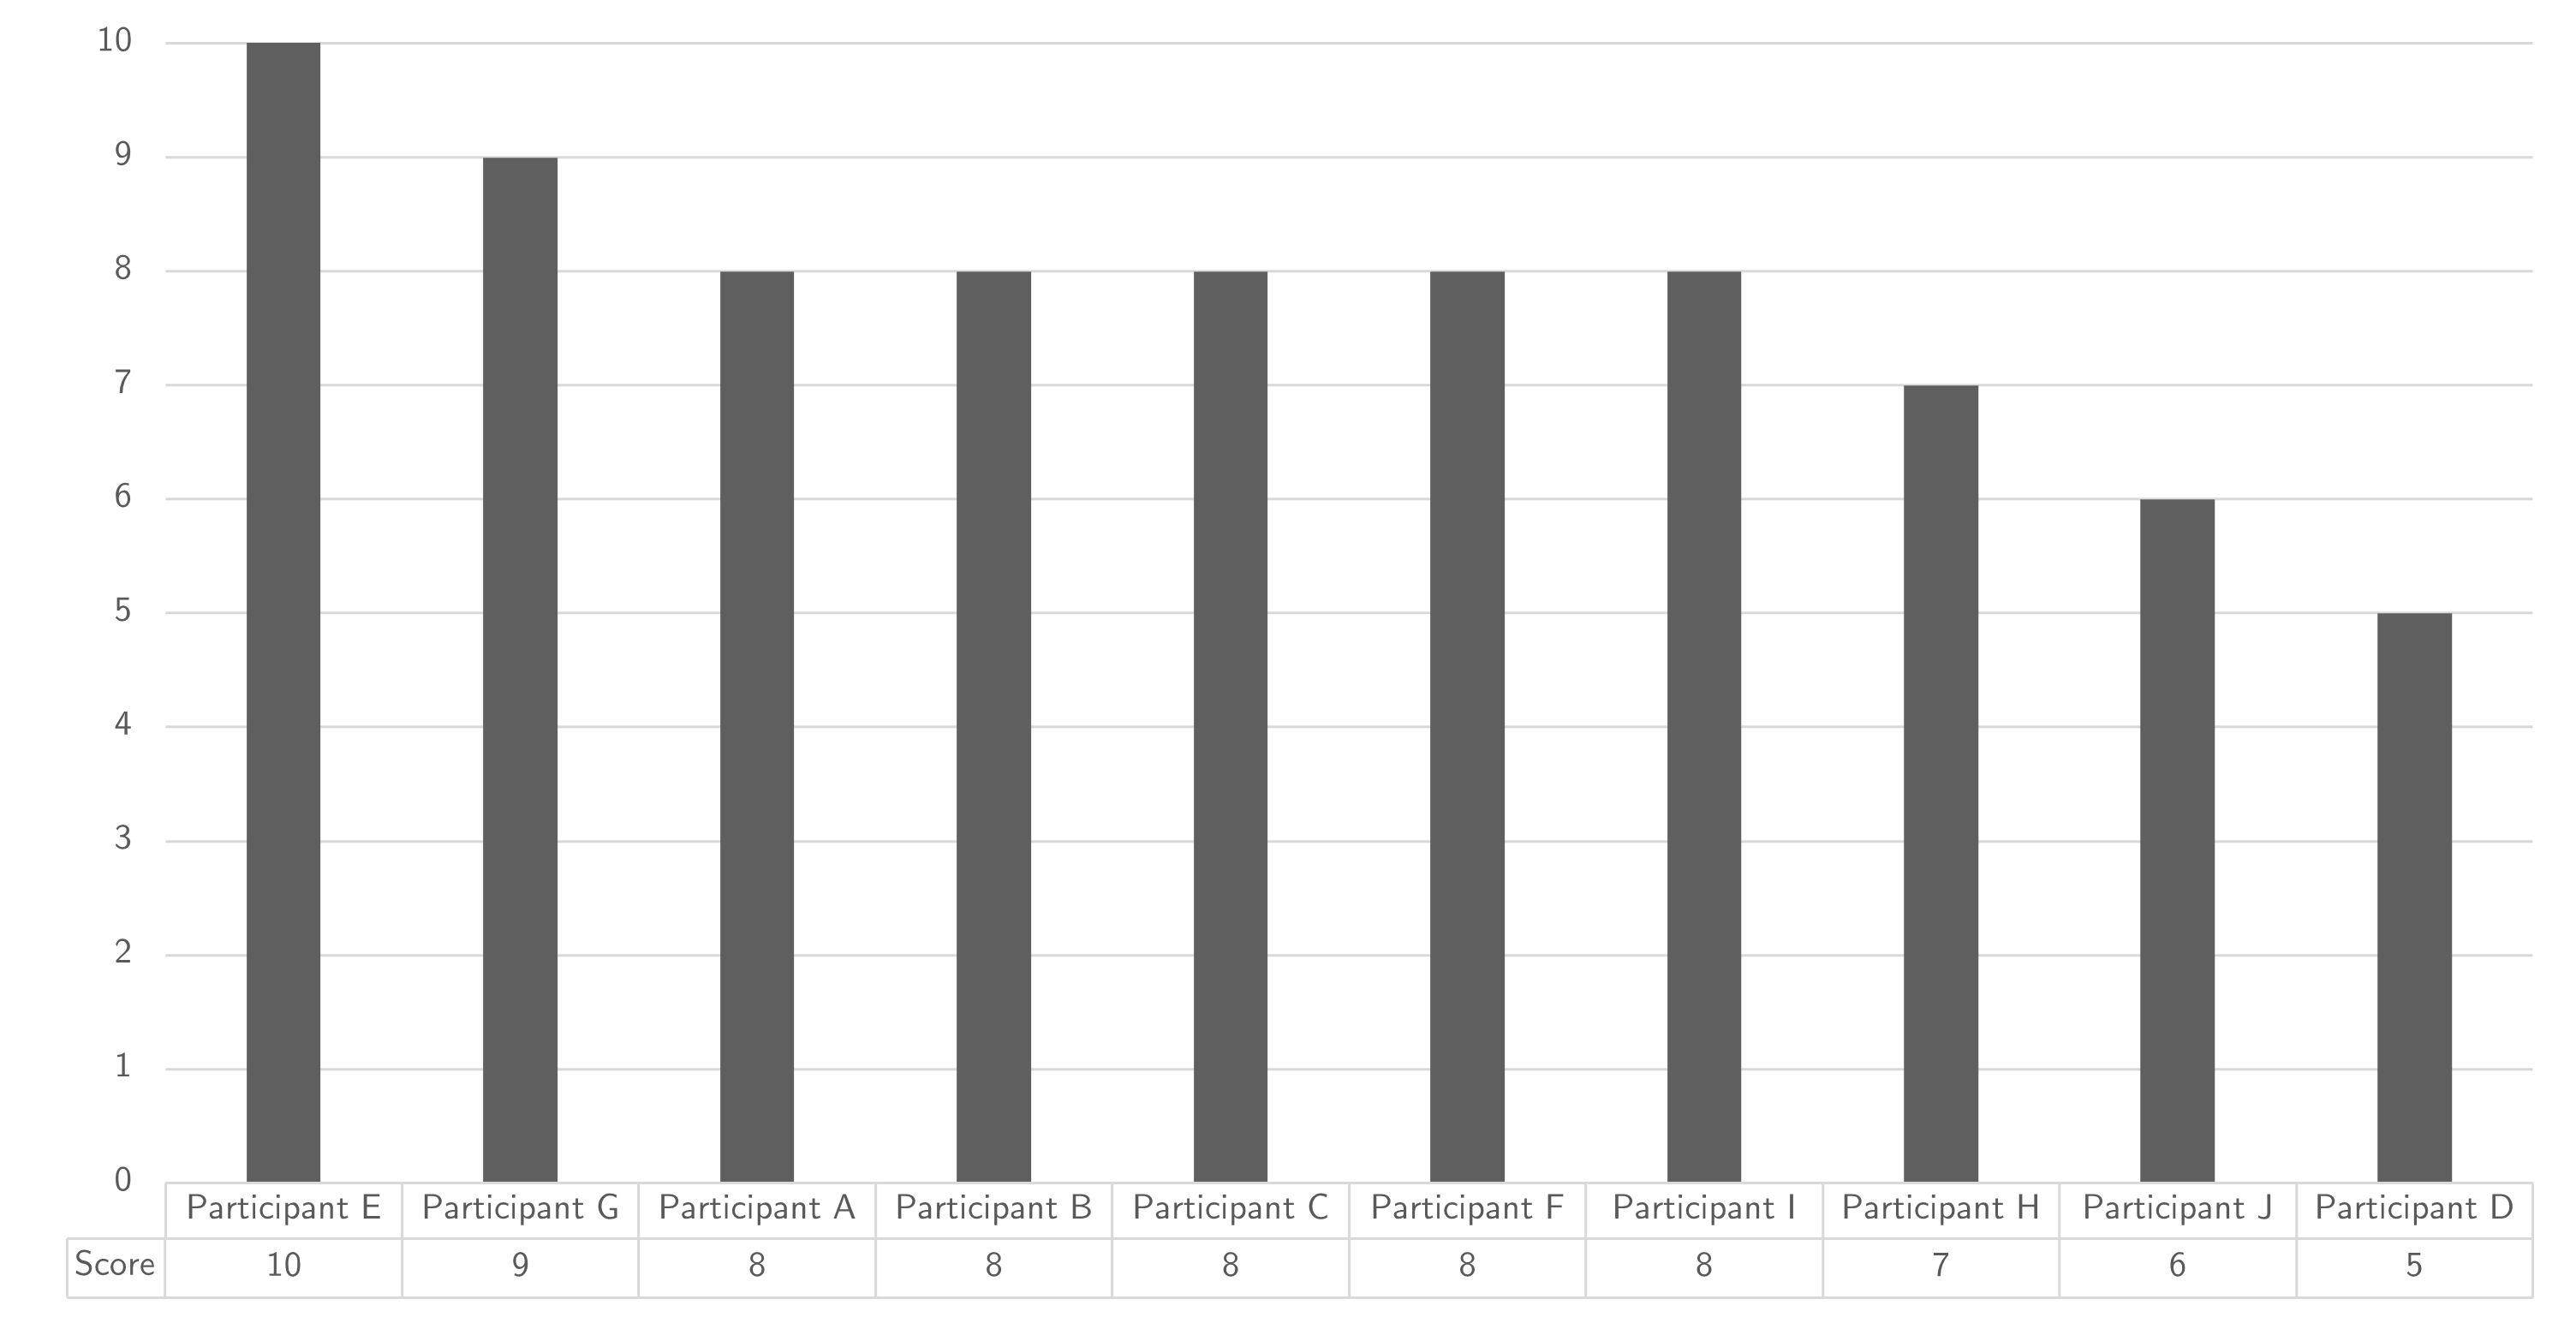
\includegraphics[width=0.9\linewidth]{images/scoreeaintraorganisationalcoherency}
	\caption[Scoring of EA attribute Intra-Organisational coherency]{Scoring of EA attribute Intra-Organisational coherency}
	\label{fig:appscoringeaintraorganisationalcoherency}
\end{figure}
\begin{table}[h!]
	\centering
	\begin{tabular}{p{.55\textwidth}ccc}
		\toprule
		\textbf{Attribute} & \textbf{Rating} & \textbf{Variability} & \textbf{Abstains} \\
		\midrule
		Intra-organisational coherency & 6,4 & 31\% & 0 \\%
		\bottomrule
	\end{tabular}%
	\caption[Scoring of EA attribute Intra-Organisational coherency]{Scoring of EA attribute Intra-Organisational coherency}
	\label{tab:appscoringeaintraorganisationalcoherency}%
\end{table}%
\newpage
\subsection{System-in-Environment Co-Evolution learning}
\begin{figure}[h!]
	\centering
	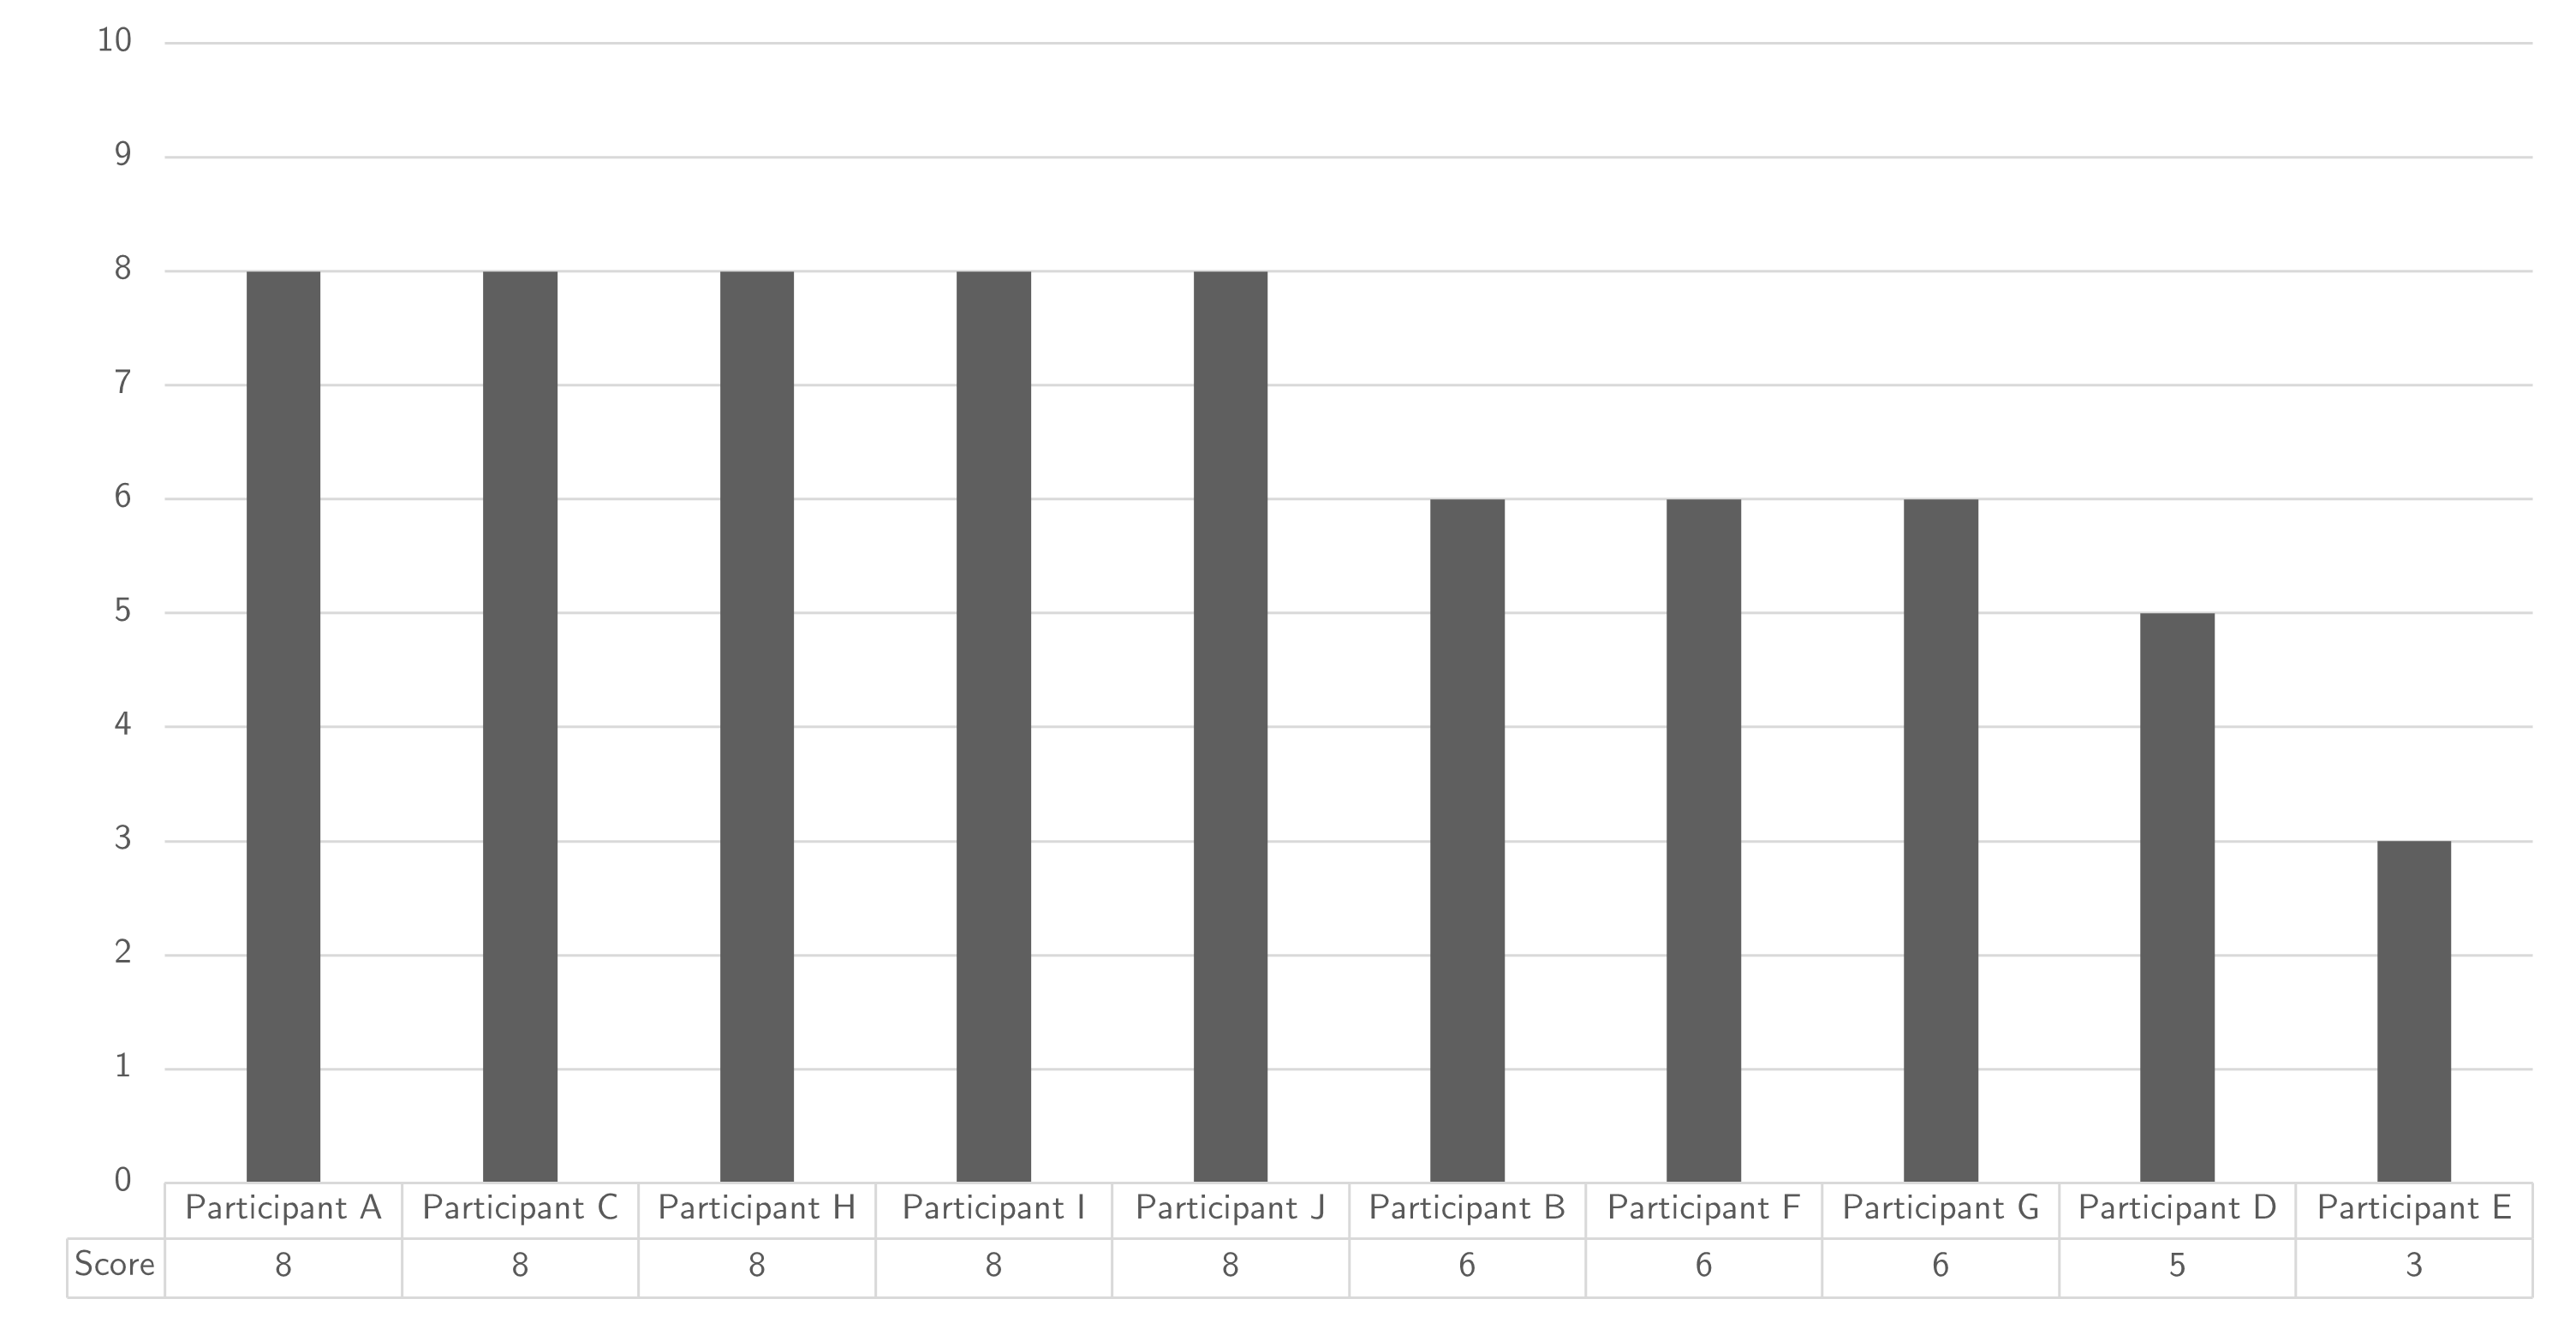
\includegraphics[width=0.9\linewidth]{images/scoreeasysteminenvironmentcoevolution}
	\caption[Scoring of EA attribute System-in-Environment Co-Evolution learning]{Scoring of EA attribute System-in-Environment Co-Evolution learning}
	\label{fig:appscoringeasysteminenvironmentcoevolutionlearning}
\end{figure}
\begin{table}[h!]
	\centering
	\begin{tabular}{p{.55\textwidth}ccc}
		\toprule
		\textbf{Attribute} & \textbf{Rating} & \textbf{Variability} & \textbf{Abstains} \\
		\midrule
		System-in-environment coevolution learning & 6,6 & 36\% & 0 \\%
		\bottomrule
	\end{tabular}%
	\caption[Scoring of EA attribute System-in-Environment Co-Evolution learning]{Scoring of EA attribute System-in-Environment Co-Evolution learning}
	\label{tab:appscoringeasysteminenvironmentcoevolutionlearning}%
\end{table}%
\newpage
\subsection{Adapt to business language}
\begin{figure}[h!]
	\centering
	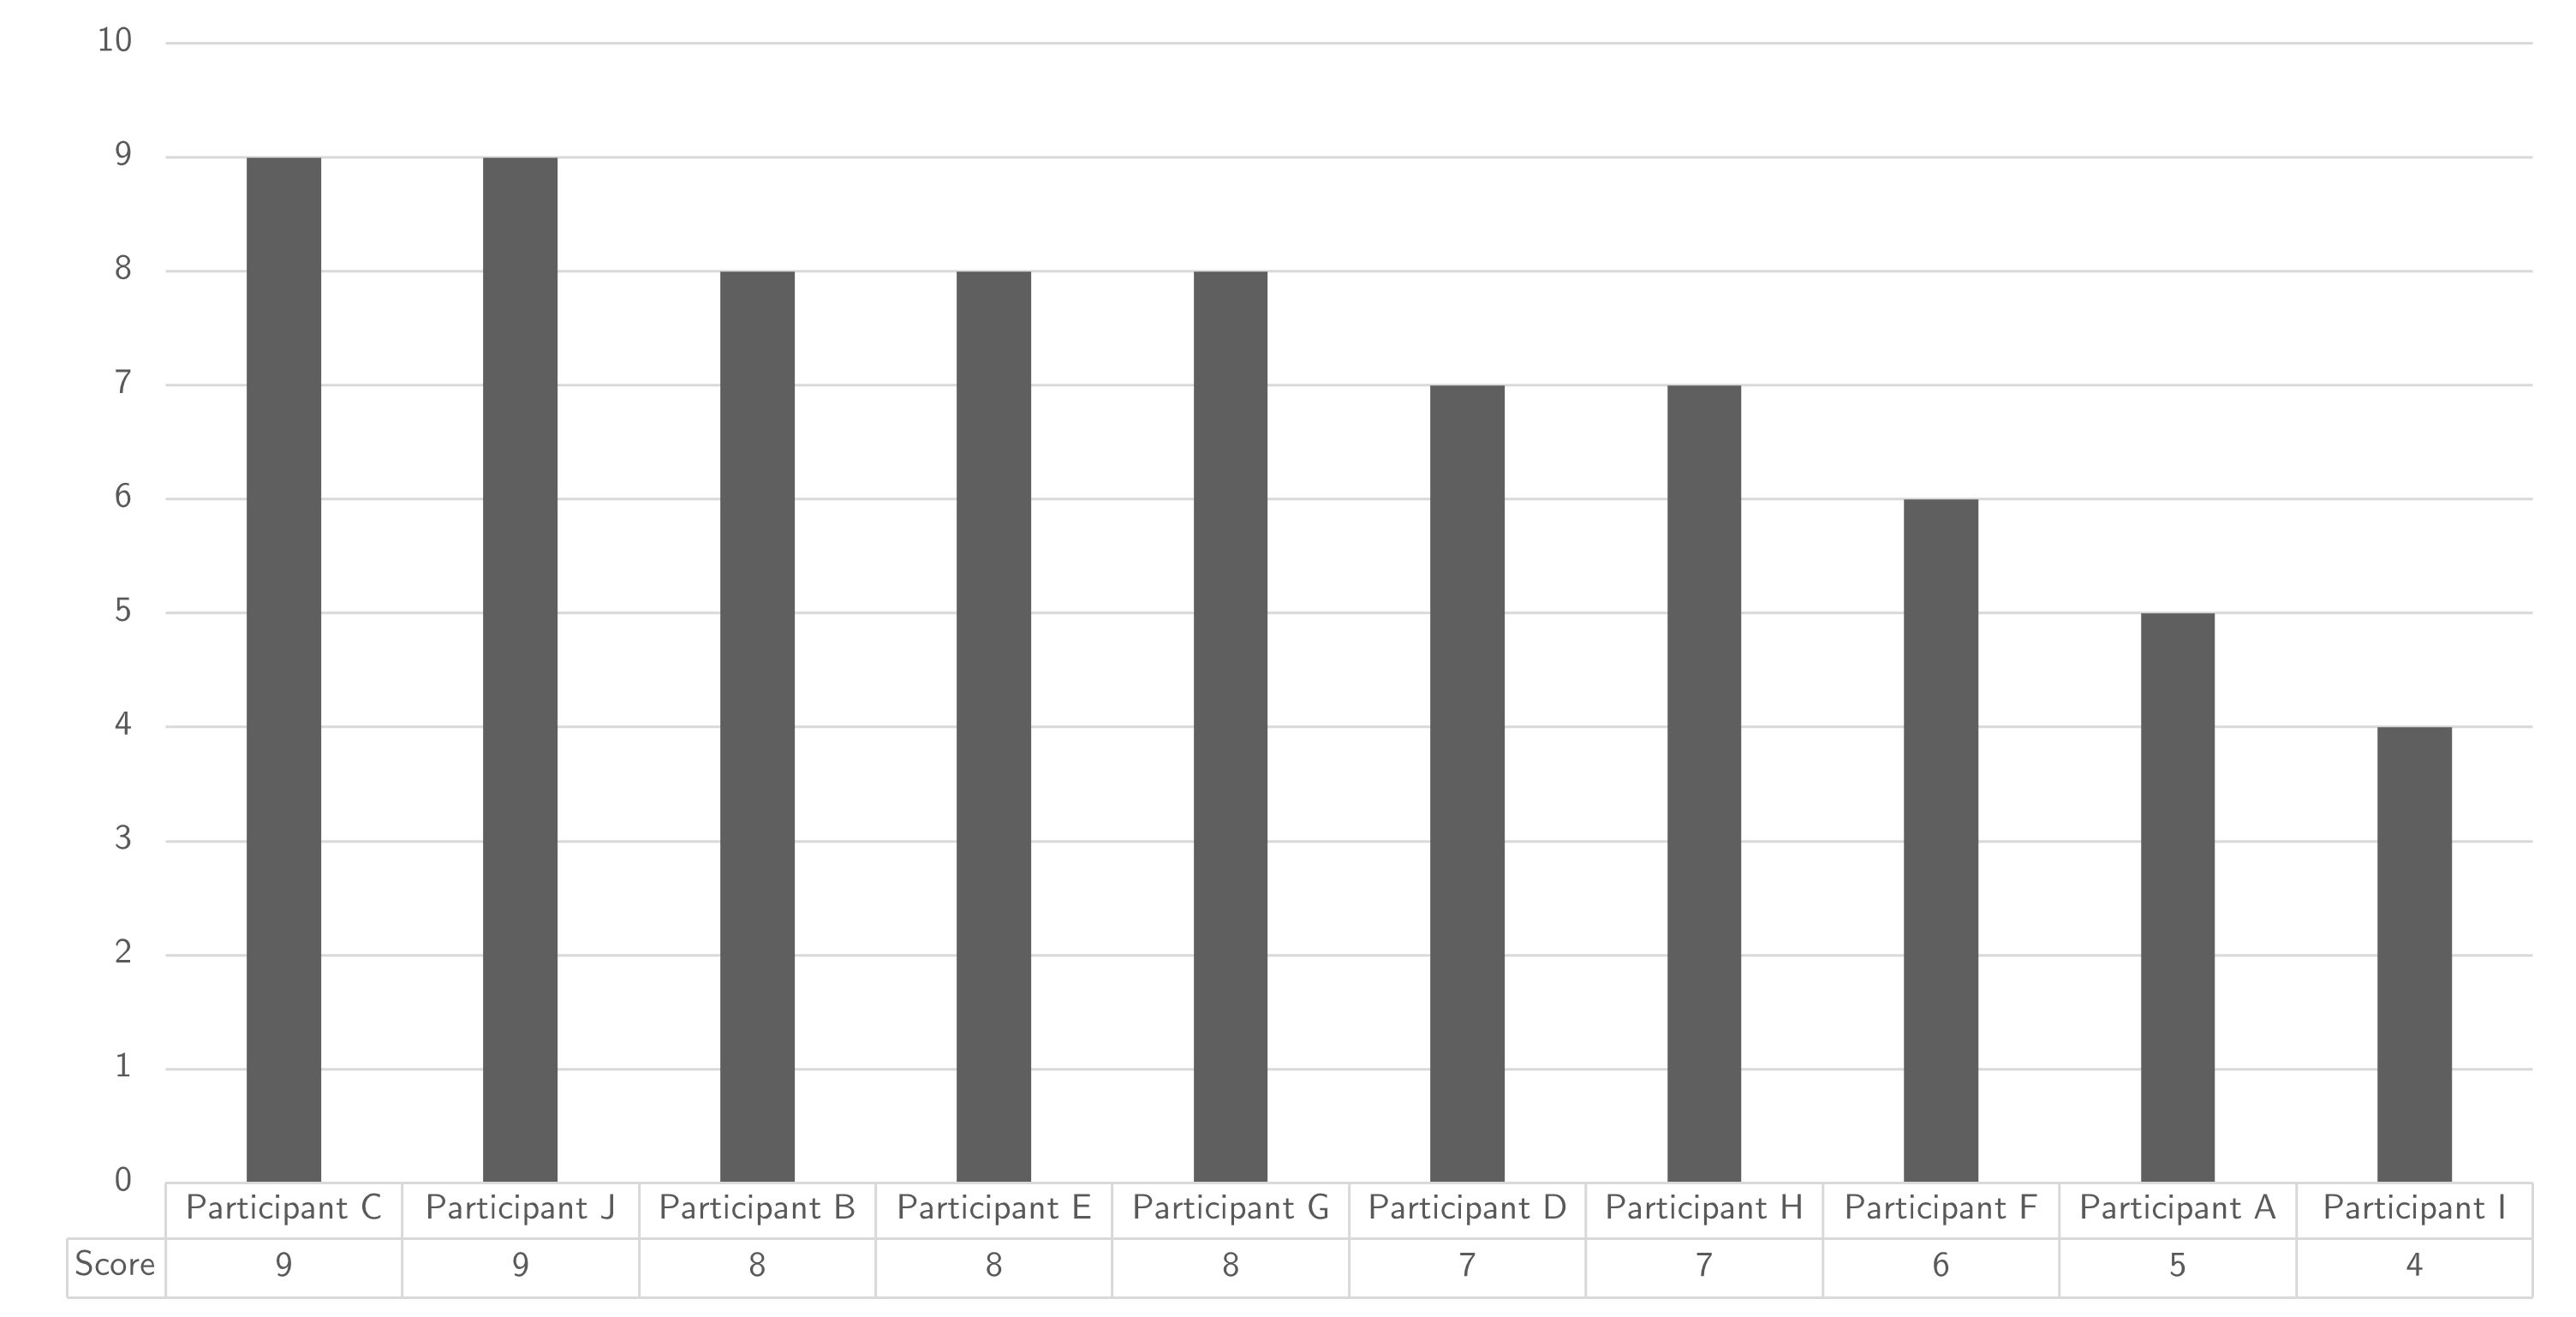
\includegraphics[width=0.9\linewidth]{images/scoreeaadapttobusinesslanguage}
	\caption[Scoring of EA attribute adapt to business language]{Scoring of EA attribute adapt to business language}
	\label{fig:appscoringeaadapttobusinesslanguage}
\end{figure}
\begin{table}[h!]
	\centering
	\begin{tabular}{p{.55\textwidth}ccc}
		\toprule
		\textbf{Attribute} & \textbf{Rating} & \textbf{Variability} & \textbf{Abstains} \\
		\midrule
		Adapt to business language & 7,1 & 35\% & 0 \\%
		\bottomrule
	\end{tabular}%
	\caption[Scoring of EA attribute adapt to business language]{Scoring of EA attribute adapt to business language}
	\label{tab:appscoringeaadapttobusinesslanguage}%
\end{table}%
\newpage
\subsection{Agile Enterprise}
\begin{figure}[h!]
	\centering
	\includegraphics[width=0.9\linewidth]{images/scoreeaagileenterprise}
	\caption[Scoring of EA attribute Agile Enterprise]{Scoring of EA attribute Agile Enterprise}
	\label{fig:appscoringeaagileneterprise}
\end{figure}
\begin{table}[h!]
	\centering
	\begin{tabular}{p{.55\textwidth}ccc}
		\toprule
		\textbf{Attribute} & \textbf{Rating} & \textbf{Variability} & \textbf{Abstains} \\
		\midrule
		Agile Enterprise & 6,4 & 50\% & 0 \\%
		\bottomrule
	\end{tabular}%
	\caption[Scoring of EA attribute Agile Enterprise]{Scoring of EA attribute Agile Enterprise}
	\label{tab:appscoringeaagileenterprise}%
\end{table}%
\newpage
\subsection{Real Time Trust}
\begin{figure}[h!]
	\centering
	\includegraphics[width=0.9\linewidth]{images/scoreearealtimetrust}
	\caption[Scoring of EA attribute Real Time Trust]{Scoring of EA attribute Real Time Trust}
	\label{fig:appscoringearealtimetrust}
\end{figure}
\begin{table}[h!]
	\centering
	\begin{tabular}{p{.55\textwidth}ccc}
		\toprule
		\textbf{Attribute} & \textbf{Rating} & \textbf{Variability} & \textbf{Abstains} \\
		\midrule
		Real Time Trust (Policy \& Attribute based) & 5,6 & 54\% & 1 \\%
		\bottomrule
	\end{tabular}%
	\caption[Scoring of EA attribute Real Time Trust]{Scoring of EA attribute Real Time Trust}
	\label{tab:appscoringearealtimetrust}%
\end{table}%
\newpage
\subsection{Foster Dialogue}
\begin{figure}[h!]
	\centering
	\includegraphics[width=0.9\linewidth]{images/scoreeafosterdialogue}
	\caption[Scoring of EA attribute Foster Dialogue]{Scoring of EA attribute Foster Dialogue}
	\label{fig:appscoringeafosterdialogue}
\end{figure}
\begin{table}[h!]
	\centering
	\begin{tabular}{p{.55\textwidth}ccc}
		\toprule
		\textbf{Attribute} & \textbf{Rating} & \textbf{Variability} & \textbf{Abstains} \\
		\midrule
		Foster Dialogue & 6,9 & 32\% & 0 \\%
		\bottomrule
	\end{tabular}%
	\caption[Scoring of EA attribute Foster Dialogue]{Scoring of EA attribute Foster Dialogue}
	\label{tab:appscoringeafosterdialogue}%
\end{table}%
\newpage
\subsection{Validation}
\begin{figure}[h!]
	\centering
	\includegraphics[width=0.9\linewidth]{images/scoreeavalidation}
	\caption[Scoring of EA attribute Validation]{Scoring of EA attribute Validation}
	\label{fig:appscoringeavalidation}
\end{figure}
\begin{table}[h!]
	\centering
	\begin{tabular}{p{.55\textwidth}ccc}
		\toprule
		\textbf{Attribute} & \textbf{Rating} & \textbf{Variability} & \textbf{Abstains} \\
		\midrule
		Validation & 7,4 & 24\% & 0 \\%
		\bottomrule
	\end{tabular}%
	\caption[Scoring of EA attribute Validation]{Scoring of EA attribute Validation}
	\label{tab:appscoringeavalidation}%
\end{table}%
\newpage
\subsection{Always fitting Enterprise Architecture}
\begin{figure}[h!]
	\centering
	\includegraphics[width=0.9\linewidth]{images/scoreeaalwaysfitea}
	\caption[Scoring of EA attribute Always fitting EA]{Scoring of EA attribute Always fitting EA}
	\label{fig:appscoringeaalwaysfitea}
\end{figure}
\begin{table}[h!]
	\centering
	\begin{tabular}{p{.55\textwidth}ccc}
		\toprule
		\textbf{Attribute} & \textbf{Rating} & \textbf{Variability} & \textbf{Abstains} \\
		\midrule
		Always fitting EA & 5,8 & 46\% & 1 \\%
		\bottomrule
	\end{tabular}%
	\caption[Scoring of EA attribute Always fitting EA]{Scoring of EA attribute Always fitting EA}
	\label{tab:appscoringeaalwaysfitea}%
\end{table}%




\section{Closing Survey}
\begin{table}[!h]
	\centering
	\begin{tabular}{p{.55\textwidth}ccc}
		\toprule
		\textbf{Question} & \textbf{Rating} & \textbf{Variability} & \textbf{Abstains} \\
		\midrule
		To what extent do you find the research relevant? & 8,2 & 23\% & 0 \\%
		To what extent did this session fulfil your expectations? & 8 & 24\% & 0 \\%
		To what extent do you think that the research can be used by yourself? & 7,7 & 10\% & 0 \\%
		To what extent do you think that the research can be used in the public sector? & 7,2 & 32\% & 1 \\%
		To what extent do you think that the research can be used by your organisation? & 6,6 & 33\% & 0 \\%
		
		\bottomrule
	\end{tabular}%
	\caption{Closing Survey}
	\label{tab:appclosingsurvey}%
\end{table}%

\section{Follow-Up Survey}
\begin{table}[!h]
	\centering
	\begin{tabular}{p{.55\textwidth}ccc}
		\toprule
		\textbf{Question} & \textbf{Rating} & \textbf{Variability} & \textbf{Abstains} \\
		\midrule
		I want to receive possible updates on this research. & 9 & 0\% & 1 \\%
		I want to know when the thesis is published. & 9 & 0\% & 1 \\%
		\bottomrule
	\end{tabular}%
	\caption{Follow-up Survey}
	\label{tab:appfollowupsurvey}%
\end{table}%
		%\chapter{All the literature}

\citeall[\fullcite]
\printbibliography[category=citeall]
		\chapter{Research Log}
\label{app:researchlog}

\begin{table}[!h]
	\begin{center}
		\begin{tabularx}{\textwidth}{@{}lX@{}}
			\toprule
			\textbf{Date} & \textbf{What} \\ \midrule%
			24/11/20 & Initial research subject proposal to AMS \\%
			25/11/20 & Initial research subject proposal sent to Hans Mulder \& Yuri Bobbert \\%
			30/11/20 & First meeting with Hans Mulder to explore the subject \\%
			12/02/21 & AMS Master Project Coaching \\%
			10/03/21 & Second meeting with Hans Mulder. Definitive Area of Research selected. The success factors of EA for Business Agility/Resilience/antifragility \\%			
			11/03/21 & Elaborated with COO on antifragility \\%
			14/03/21 & Started research on the concept of antifragility \\%
			03/04/21 & One Pager on the concepts Enterprise Architecture, Public Sector, Independant Software Vendor, and Antifragility \\%			
			04/04/21 & Deskresearch on concepts \\%			
			10/04/21 & Reading Taleb \\%			
			25/05/21 & Third meeting with Hans Mulder \\%	
			20/06/21 & Creating 5 pager \\%
			20/06/21 & Sent 5 pager presentation for review to Hans Mulder \\%
			20/06/21 & Sent 5 pager presentation for review to Dieneke Schouten (COO) and Maarten Hillenaar (CEO) \\%
			20/06/21 & Promotor suggestion Roland Ettema, Martin Op 't Land, Bas van Gils or Hans Mulder \\%
			20/06/21 & Sugestion of Hans Mulder as promotor with Edzo Botjes as co-promotor \\%
			21/06/21 & Requested Maarten Hillenaar as Sponsor, Dieneke Schouten as Second Reader, Jan Ploeg as participant in Delphi, Christiaan Konstapel as interviewee \\%			
			24/06/21 & Presentation of Five Pager at Master Project Coaching AMS \\%
			29/06/21 & Created thesis LaTeX skeleton  \\%			
			06/07/21 & Meeting with Edzo Botjes to get acquainted \\%	
			06/07/21 & Edzo Botjes accepted co-promotorship \\%
			date    & what \\%
			date    & what \\%
			date    & what \\%
			enddate & final version \\ \bottomrule
		\end{tabularx}
		\label{tab:researchlog}
	\end{center}
\end{table}
	\end{appendices}

\end{document}